% reducesymm/QFT/finiteQED.tex
% Predrag  switched to github.com               jul  8 2013
%%%%%%%%%%%%%%%%%%%%%%%%%%%%%%%%%%%%%%%%%%%%%%%%%%%%%%%%%%%%%%%%%%%%%%%%%

\chapter{Is QED finite?}
\label{c-finiteQED}

\begin{bartlett}{
For Emily, after she gets bored with ``Baby Loves Quarks.''
        }
%\bauthor{
%Feynman's challenge, 12th Solvay Conference\rf{Feynman62}
%    }
\end{bartlett}
\bigskip

\noindent
%\item[2017-04-28
In 2017 Laporta\rf{Laporta17,Laporta18} completed the twenty-year
project of computing analytically the individual contributions
of 891 4-loop vertex diagrams contributing to the electron
magnetic moment $g$. Vertex diagrams separate
in 25 gauge sets (see \reffig{Laporta17figuragau}).
The numerical contribution of each set is
listed in \reftab{Laporta17:tableset}.
Adding only the quenched set $V$ diagrams (diagrams with no lepton
loops, see \reffig{Cvit77bFig3} %\reftab{tabGaugeSets}
and \ref{Laporta17figuragauShort}), one
finds for the 4- and 5-loop contributions to the anomaly
$a[V]=\left.\frac{1}{2}(g-2)\right|_V$:
\bea
 a^{(8)}[V] &=& -2.176866027739540077443259355895893938670
\continue
        &=& -2.17\dots \,\qquad \mbox{ Aoyama \etal\ 2012\rf{AoHaKiNi12}}
\continue
        &\approx& 0 \,\qquad\qquad\quad\quad \mbox{Cvitanovi\'c 1977\rf{Cvit77b}}
\continue
 a^{(10)}[V] &=& 7.606(192)\dots \,\; \mbox{   Aoyama \etal\ 2018\rf{AoKiNi18}}
\continue
             &=& 6.782(113)\dots \,\; \mbox{   Volkov 2019\rf{Volkov19}}
\continue
        &\approx& 3/2  \,\qquad\qquad\quad \mbox{Cvitanovi\'c 1977\rf{Cvit77b}}
\,.
\label{anomalValues}
\eea
%Closed electron loops only:
%\begin{align}
% \aql{4}&=  \phantom{+}0.264620262813094503290612188456063884609 \,.
%\end{align}
There is a prediction dating back to 1977 for values of these terms: the
predicted $a^{(8)}[V] \approx 0$ does not pan out,
but the difference is small, considering that this
is a sum of 518 vertex diagrams (or 47 self-energy
diagrams)\rf{KinLin90}.
Likewise, the prediction for $a^{(10)}[V]$ is not too far off, considering
that this is a sum of 6\,354 vertex diagrams of \reftab{Cvit77bTab1} (or
389 self-energy diagrams).

\section{Electron magnetic moment}
\label{sect:magMom}

\noindent
% pasted from BAGTB17
This section sets up the notation - the reader can safely skip it and
start with \refsect{sect:finitness}. For an introduction to the
conventional magnetic moment calculation, see for example the
Cvitanovi\'c online graduate QFT course, lectures 25 and 26
\HREF{http://chaosbook.org/~predrag/courses/PHYS-7147-13/schedule.xml}
{here}.

An electron of mass $m$  has a magnetic moment
\beq
\mu=\frac{e\hbar}{2mc}\,\frac{g}{2}
\ee{Laporta18(1)}
where $g$ is the gyromagnetic ratio.
In Dirac theory\rf{Dirac28}, the electron has $g=2$.

Consider the electron-photon vertex $\Gamma_{\mu}$ of quantum
electrodynamics, with $p_{i}=p-q/2$ and $p_{o}=p+q/2$ the momenta of
incoming and outgoing electron lines, evaluated on the electron mass
shell $p_{i}^2=p_{o}^2=m^2$.
By Gordon decomposition the vertex can be written in terms of the Dirac
and Pauli form factors $F_1(q^2)$ and $F_2(q^2)$:
\beq
\overline{u}(p_{o}) \Gamma_{\mu}(p,q) %\Big|_{k^2=p^2=m^2}
u(p_{i})
    =    %    && \hspace{-4.5cm}
\overline{u}(p_{o}) \Bigg\{ F_1(q^2) \gamma_{\mu} -
\frac{F_2 (q^2)}{2m} \; \sigma_{\mu \nu} q^{\nu} \Bigg\} u(p_{i}) \,,
\label{BAGTB17(35-1)}
\eeq
where the spinors  $\overline{u}(p_{i})$ and $u(p_{i})$  satisfy the Dirac
equation:
\[
\overline{u}(p_{o}) \not\!{p}_{o} = m \, \overline{u}(p_{o})
\,, \qquad
\not\!{p}_{i} \, u(p_{i})  =  m \, u(p_{i}) \,.
\]
We follow the notation of Bjorken and Drell\rf{BjoDre65}
and Cvitanovi{\'c} and Kinoshita\rf{CviKin74c}.
$Z_1$,
$Z_2$, and % = (1-B)^{-1}$, and
$Z_3$,
are the respectively the vertex,
the electron wave function, and
the photon wave function
renormalization constants,
and the electron mass will be set to $m = 1$ throughout.
In what follows it is convenient to define $Z_1=1+L$.
For QED the charge conservation requires that the renormalized charge
form factor satisfies $\tilde{F}_1(0) = 1$, which is guaranteed by the
Ward identity\rf{Ward50}
$Z_1=Z_2$.
%The renormalized $\tilde{\Gamma}^{\nu}(p,q)$ and unrenormalized
%$\Gamma^{\nu}(p,q)$
%proper vertex are related by the electron wave function renormalization constant
%\beq
%\tilde{\Gamma}^{\nu} =Z_2 \Gamma^{\nu} = \Gamma^{\nu}/(1-B)
%\,.
%\ee{PRD10-74-III(2.1)}
The vertex renormalization constant $L$ is given by the
on-shell value of the unrenormalized charge form factor\rf{BroSul67}
    \PC{2018-11-26
    Brodsky and Sullivan\rf{BroSul67} is not an obvious reference - they
    just state the trace formulas, no derivation or attribution
    }
\beq
1+L = F_1(0)
    = \frac{1}{4}\tr\left[(\not\!{p}+1)p^{\nu}\Gamma^{\nu}\right]_{q=0}
\label{PRD10-74-III(2.3)}
\,,
\eeq
and  $a = (g-2)/2$, the anomalous magnetic moment of an electron is
given by the static limit of the magnetic form factor
$a=\tilde{F}_2(0)=M/(1+L)$, where\rf{BroSul67}
\beq
M = \lim_{q\to0}
% \frac{1}{4p^4q^2} % simplified by P^2=1
\frac{1}{4q^2}
\tr\left\{
\left[\gamma^{\nu}p^2-(1+q^2/2)p^{\nu}\right]
(\not\!{p}_o+1)\Gamma_{\nu}(\not\!{p}_i+1)
\right\}
\label{PRD10-74-III(2.2)}
\,.
\eeq
The perturbative expansions for the
magnetic moment anomaly is defined as %\rf{CviKin74c}
\beq
a = \frac{M(\alpha_0)}{1+L(\alpha_0)}
  =  \sum_{n=1}^\infty
          a_{0}^{(2n)}\left(\frac{\alpha_0}{\pi}\right)^{n}
\,,
\ee{IRstruct(1)}
where $1+L =F_1(0)$, $M=F_2(0)$ are computed from the unrenormalized
proper vertex \refeq{BAGTB17(35-1)}, given by the sum of all one-particle
irreducible electron-electron-photon vertex diagrams with internal
photons, electron loops and electron mass counterterms.
Expanding $M$ and $L$ we have
\bea
a_{0}^{(2)} &=& M^{(2)}
            \continue
a_{0}^{(4)} &=& M^{(4)} - L^{(2)}M^{(2)}
            \label{PRD10-74-III(2.6)}\\
a_{0}^{(6)} &=& M^{(6)} - L^{(2)}M^{(4)} - (L^{(4)} - (L^{(2)})^2) M^{(2)}
\nnu
\eea

As shown in \refref{IRstruct}, for the anomaly \refeq{IRstruct(1)}
expressed in terms of the unrenormalized coupling constant $\alpha_0$,
all $a_{0}^{(n)}$ are IR finite, for both QED and QCD.
The UV finite expression for the anomaly \refeq{IRstruct(1)} is obtained
by the charge renormalization
\beq
\alpha=Z\alpha_0
\,,\qquad
Z= \frac{Z_2}{Z_1}\,Z_3
\,,
\ee{IRstruct(3)}
where
$Z_1$,
$Z_2$, and
$Z_3$
%renormalization constants
are computed as power series in the bare coupling constant $\alpha_0$.
For QED $Z_1=Z_2$ by the Ward identity\rf{Ward50}, and for QCD the $Z_i$'s are
related by the Taylor-Slavnov\rf{Taylor71,Slavnov72} identities
\refeq{IRstruct(3)}. The simple structure of \refeq{IRstruct(1)} and
\refeq{PRD10-74-III(2.6)} should simplify the worldline calculations of
\refsect{sect:magMomWorldline}.

The Dirac equation predicts that the magnetic moment of an
electron of charge $e$ and mass $m$ is ${ {\mu}} = {e}/{2 m} $,
\ie, in the absence of radiative corrections
$\tilde{F}_1(0)=1$ and $\tilde{F}_2(0)=0$. In 1948 Schwinger\rf{Schwinger48} showed that in
the leading, one-loop order in the fine structure constant $\alpha$, the
radiative corrections lead to the anomalous magnetic moment of form
$\tilde{F}_2(0)={\alpha}/{2\pi}+ a^{(2)}\left({\alpha}/{\pi}\right)^2 +
\cdots$
(the result engraved on Schwinger's
\HREF{https://en.wikipedia.org/wiki/Julian_Schwinger\#/media/File:Julian_Schwinger_headstone.JPG}
{tombstone}).
%\[
% \frac{e}{2 m} \Rightarrow
% \left( 1 + \frac{1}{2} \left(\frac{\alpha}{\pi}\right) \right) \frac{e}{2 m}.
%\]
These notes are about what to expect for the $\left({\alpha}/{\pi}\right)^n$
term in this series.

%%%%%%%%%%%%%%%%%%%%%%%%%%%%%%%%%%%%%%%%
\begin{figure}
\begin{center}
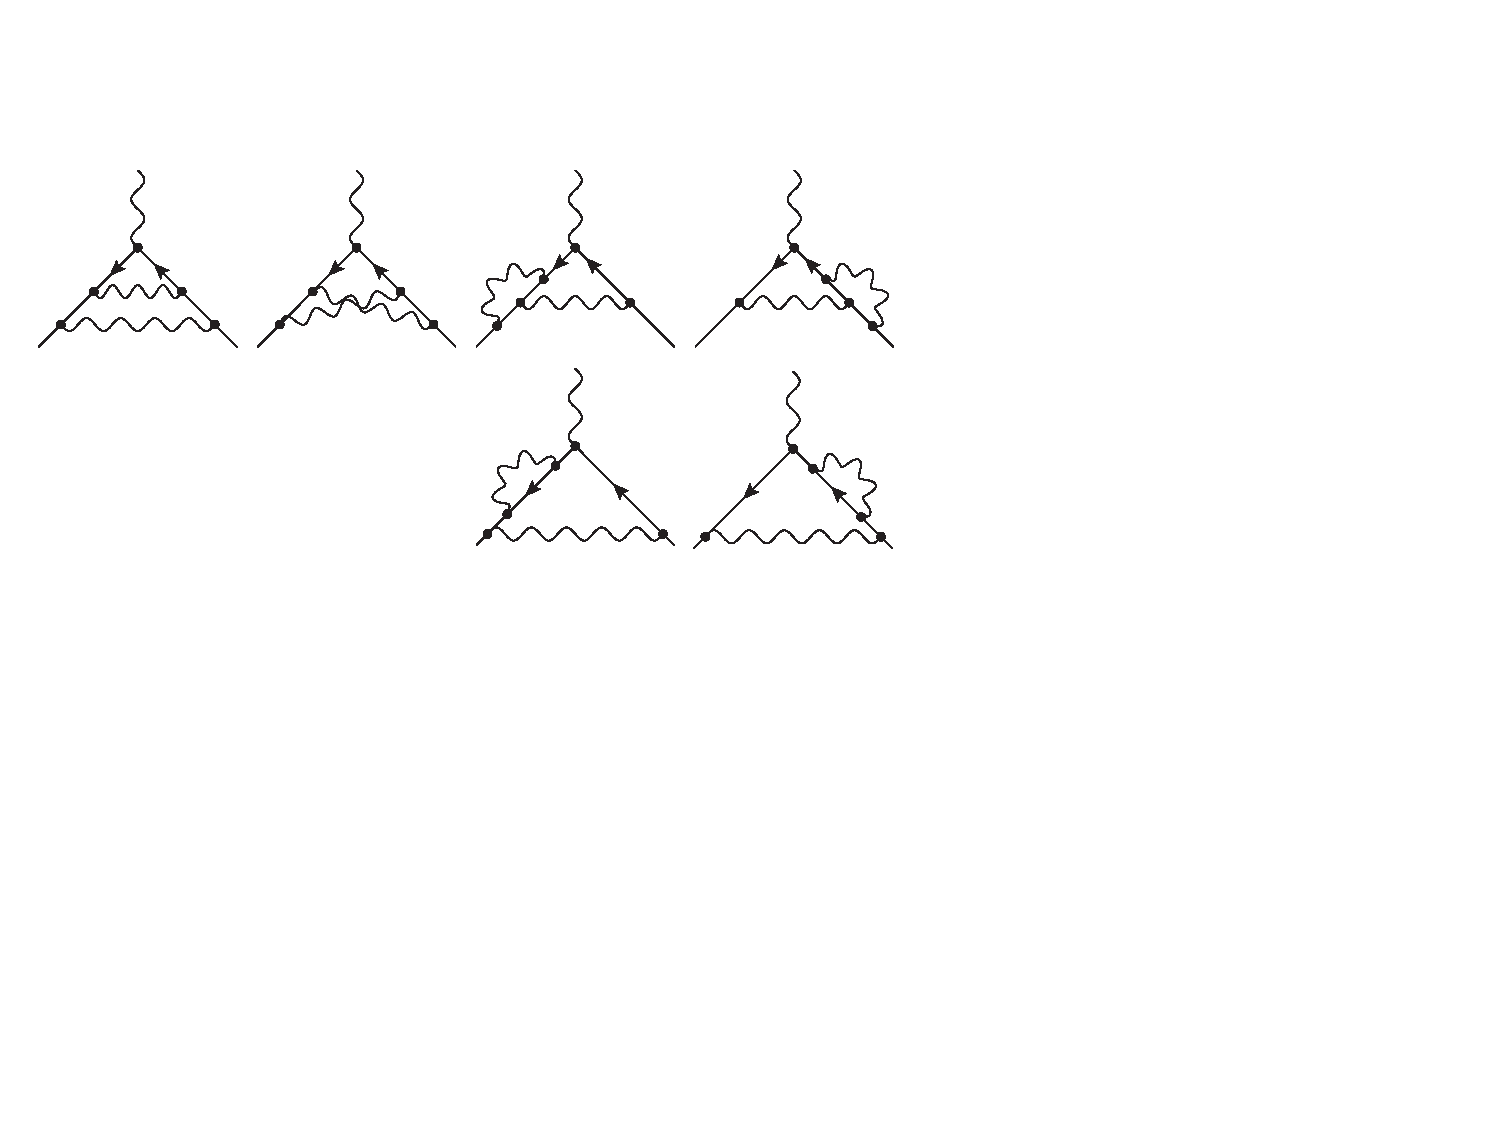
\includegraphics[width=0.50\textwidth]{Volkov18twoLoopsQ}
\end{center}
\caption{\label{Volkov18twoLoops}
The two-loop vertex diagrams contributing to $a^{(4)}[V]$ magnetic moment
anomaly.
From Volkov\rf{Volkov18}.
}
 \end{figure}
%%%%%%%%%%%%%%%%%%%%%%%%%%%%%%%%%%%%%%%%



\section{Gauge sets}
\label{sect:finitness}

\begin{bartlett}{
Is there any method of computing the anomalous moment of the
electron which, on first approximation, gives a fair approximation to the
$\alpha$ term and a crude one to $\alpha^2$; and when improved, increases
the accuracy of the $\alpha^2$ term, yielding a rough estimate to
$\alpha^3$ and beyond?
        }
\bauthor{
Feynman's challenge, 12th Solvay Conference\rf{Feynman62}
    }
\end{bartlett}

\bigskip

%%%%%%%%%%%%%%%%%%%%%%%%%%%%%%%%%%%%%%%%
\begin{figure}
\begin{center}
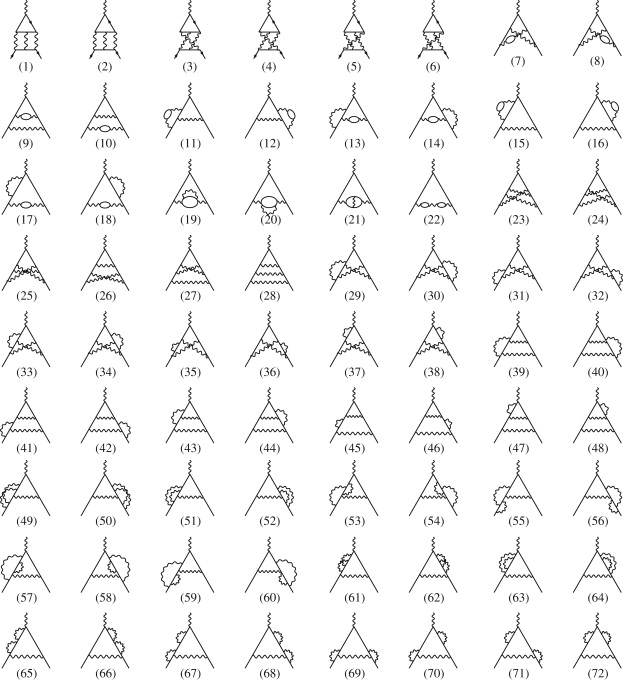
\includegraphics[width=1.00\textwidth]{JegNif09fig10}
\end{center}
\caption{\label{JegNif09fig10}
The three-loop vertex diagrams contributing to $a^{(6)}_1$
magnetic moment
(from Jegerlehner and Nyffeler\rf{JegNif09}).
Lautrup \etal\rf{LaPeRa72} were the first to note that
subsets
% $km'm$ =
$(3,0,0)$ = $\{23,24,25,26,27,28\}$;
$(2,1,0)$ = $\{29,31,33,35,37,39,41,43,45,47\}$ and its time-reversal
$(2,0,1)$ = $\{30,32,34,36,38,40,42,44,46,48\}$;
$(1,2,0)$ = $\{49,51,53,55,57,59,61,63,65,67\}$ and its time-reversal
$(1,0,2)$ = $\{50,52,54,56,58,60,62,64,66,68\}$;
and
$(1,1,1)$ = $\{69,70,71,72\}$
are the minimal gauge sets, see \reffig{Cvit77bFig2}.
}
 \end{figure}
%%%%%%%%%%%%%%%%%%%%%%%%%%%%%%%%%%%%%%%%

%%%%%%%%%%%%%%%%%%%%%%%%%%%%%%%%%%%%%%%%%%
\begin{table}
\begin{center}
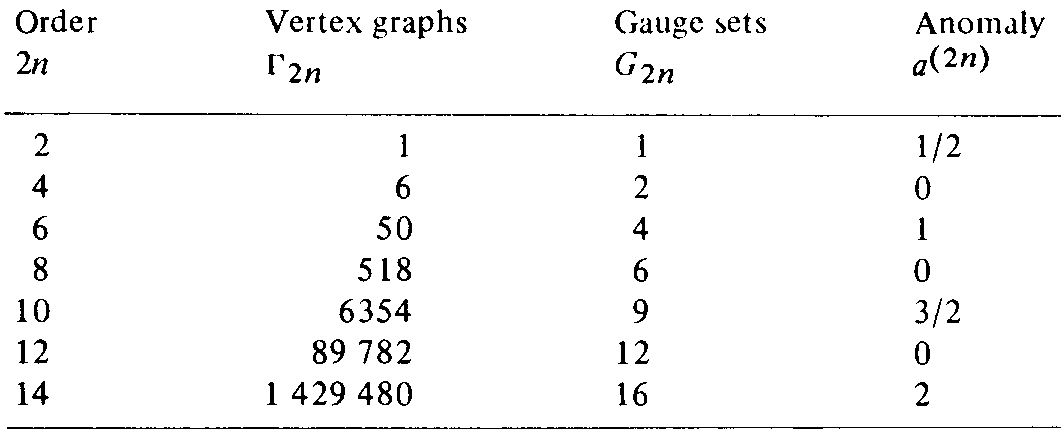
\includegraphics[width=0.80\textwidth]{Cvit77bTab1}
\end{center}
\caption{\label{Cvit77bTab1}
Comparison of the number of quenched QED vertex diagrams
(diagrams without fermion loops), gauge
sets, and the gauge-set approximation \refeq{Cvit77b(1)} for the magnetic
moment in $2n$th order.
From \refref{Cvit77b}.
}
\end{table}
%%%%%%%%%%%%%%%%%%%%%%%%%%%%%%%%%%%%%%%%%%%%%%%%%%%%%%%%%%%

% finiteQEDins.tex
% PC created from lectures/talks/DFS_pris.tex       2017-05-25
% PC with edits March 2003
% PC with edits July 1997
%Acceptance speech - 1993 NKT Research Prize in Physics
%Dansk Fysisk Selskab \AA rsm\o de, Lalandia, R\o dby, 18 maj 1993
\noindent
In 1972 Toichiro Kinoshita and Predrag Cvitanovi\'c had completed
computing a large number of 3-loop anomalous magnetic moment Feynman
diagrams and regularization counterterms\rf{CviKin72},
\reffig{JegNif09fig10}.
The subsequent 4- and 5-loop numerical and analytic calculations were
nothing short of heroic\rf{KinLin90,LapRem96,Laporta17,AoHaKiNi15,Volkov19}. The
quantum field theory was used in the standard way\rf{BjoDre65}, by
expanding the magnetic moment into combinatorially many Feynman diagrams
(see the numbers of vertex graphs in \reftab{Cvit77bTab1}).
Each Feynman diagram corresponds to an integral in many dimensions, with
oscillatory integrand with thousands of terms, each integral separately
UV divergent, IR divergent, and unphysical, as its value depends on the
definition of counterterms and the choice of gauge.
The numerical values of these integrals typically range from  $\pm 10$
to $\pm 100$. For example, the largest contributions of
the 389 quenched self-energy diagrams listed in
Aoyama \etal\ 2018\rf{AoKiNi18} are of order $\pm 20$.

Adding up hundreds of such contributions, of wildly fluctuating values,
yields (for the no-fermion loops subset $V$, in the notation of
\refref{AoHaKiNi15})
\[
 a^{(6)}[V] %\aql{6}
 \,=\, +  (0.92 \pm 0.02) \left(\frac{\alpha}{\pi}\right)^3.
\]
But why ``+'' and not ``-''? Why so small? Why does a sum of hundreds of
diagrams and counterterms yield a number of order of unity, and not 10 or
100 or any other number?

%%%%%%%%%%%%%%%%%%%%%%%%%%%%%%%%%%%%%%%%
\begin{figure}
\begin{center}
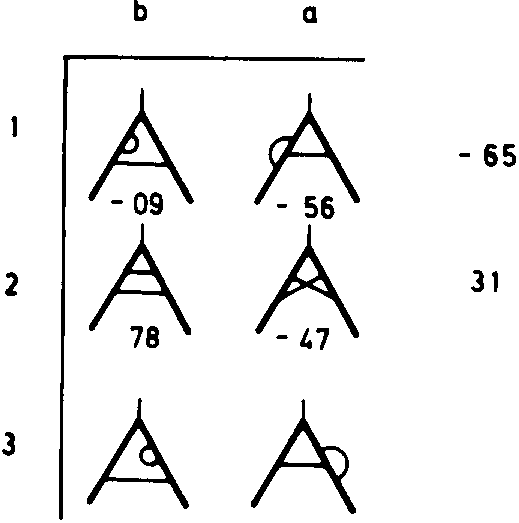
\includegraphics[width=0.50\textwidth]{Cvit77bFig1}
\end{center}
\caption{\label{Cvit77bFig1}
Rows: the fourth-order quenched QED
Columns: external field insertions into the two self-energy sets.
Rows: gauge sets
$(k,m,m')$ contributing to $a^{(4)}[V]$: (1) = $(1,1,0)$,
(2) = $(2,0,0)$
and
(3) = $(1,0,1)$.
For diagrams related by time
reversal (here (1) and (3))
the value listed under the first diagram of the pair is
the total contribution of the pair. Contributions seem to be of order
$\pm\frac{1}{3}\left(\frac{\alpha}{\pi}\right)^2$, and suggest that
a set and its time-reversed partner should be counted separately.
From \refref{Cvit77b}.
}
 \end{figure}
%%%%%%%%%%%%%%%%%%%%%%%%%%%%%%%%%%%%%%%%

If gauge invariance of QED guarantees that all UV and on-mass shell IR
divergences cancel, could it be that it also enforces cancellations among
the finite parts of contributions of different Feynman graphs?

\subsection{QED vertex photons come in three ``colors''}
\label{sect:gaugeSetDeriv}

As first noted by Lautrup, Peterman and de Rafael\rf{LaPeRa72}, the
renormalized on-mass shell QED vertex diagrams separate into a sum of
minimal gauge-invariant subsets, each subset separately UV and IR finite.
The only published proof of this elementary fact seems to be
\refref{Cvit77b}. The very reasonably priced \refref{FieldThe} might be
worth a read, especially if one is interested in the non-abelian
theories as well\rf{MassShell,IRstruct,QCDmshell},
see \refsect{sect:QCDgaugeSets}.

A gauge change generates a $k^\mu$ term in a photon propagator,
and that affects a tree electron vertex in a very simple way,
\(
\slashed{k} = (\slashed{p}+\slashed{k}+m) - (\slashed{p}+m)
\,,
\)
or, diagrammatically\rf{BjoDre65,FieldThe} (graphs drawn by H.
Ki{\ss}ler\rf{KisKre16}),
\PC{2017-07-14
need to download, put axohelp.exe, the executable version of axohelp
for MS-Windows into the directory where I can run it from, presumably
Program~Files/MiKTeX 2.9/miktex/bin/x64
}
\begin{align}
  \begin{tabular}{ccccc}
$\!{\begin{aligned}\frac{1}{\slashed{p}+\slashed{k}-m}\slashed{k}\frac{1}{\slashed{p}-m}\end{aligned}}$ &
$=$ &    $\!{\begin{aligned}\frac{1}{\slashed{p}-m}\end{aligned}}$ &
$-$ &    $\!{\begin{aligned}\frac{1}{\slashed{p}+\slashed{k}-m},\end{aligned}}$
\\
$\treeA{.45}$ & $=$ & $\treeB{.45}$ & $-$ & $\treeC{.45}$.
  \end{tabular}
  \label{KisKre16eq:treeLevel1}
\end{align}

To simplify matters, in what follows we shall consider only the
no-fermion loop diagrams, or `quenched-', or `q-type' diagrams
(`quenched', as this corresponds to the $N_f$-independent part of the
vertex amplitude in
QED with $N_f$ flavors).
The minimal gauge-invariant subsets without electron loops (see
\reffig{JegNif09fig10} diagrams $\{23-72\}$; \reffig{Cvit77bFig1};
\ref{Cvit77bFig2}; \ref{Cvit77bFig3}; and \ref{Laporta17figuragauShort})
will be hereafter be referred to as \emph{gauge sets}.

A quenched QED gauge set $(k,m,m')$ consists of all 1-particle irreducible vertex
diagrams without electron loops, with $k$ photons crossing the external
vertex (cross-photons) and $m [m']$ photons originating and terminating
on the incoming [outgoing] electron leg (leg-photons), where $m\geq m'$.
For asymmetric pairs of sets, with $m\neq m'$, the contribution to the
anomaly $a_{kmm'}$ is, in the convention of \refref{Cvit77b}, the sum of
the set and its mirror (time-reversed) image,
\beq
a[V]=\left.\frac{1}{2}(g-2)\right|_V
       =  \sum_{k=1}^\infty\sum_{m=0}^\infty\sum_{m'=0}^m
          a_{kmm'}\left(\frac{\alpha}{\pi}\right)^{k+m+m'}
\,.
\ee{quenchAnom}

\subsection{The unreasonable smallness of gauge sets}
\label{sect:gaugeSetsSmall}

When the diagrams computed in \refref{CviKin74c} are grouped into
gauge sets, \reffig{Cvit77bFig1} to \reffig{Laporta17figuragauShort},
a surprising thing happens; while the
finite part of each Feynman diagram is of order of 10 to 100, every
 gauge set known at the time added up to approximately
$$
		   \pm {1 \over 2} \left(\frac{\alpha}{\pi}\right)^n
\,,
$$
with the sign given by a simple empirical rule
\beq
a_{kmm'} = (-1)^{m+m'}\frac{1}{2}
\,.
\ee{Cvit77b(5)}
The sign rule is further corroborated by sets with photon
self-energy insertions (but with the absolute size scaled down to
$3-15\%$ of \refeq{Cvit77b(5)}).
In \reffig{Cvit77bFig3} this rule is compared with the actual numbers,
and the 1977 four-loop prediction is given\rf{Cvit77b}.
With that prediction, the ``zeroth'' order estimate of the electron
magnetic moment anomaly $a$ is given by the ``gauge-set
approximation,'' convergent and summable to all orders
\beq
a=\frac{1}{2}(g-2) =  \frac{1}{2} \frac{\alpha}{\pi}
                     \frac{1}
           {\left( 1 - \left(\frac{\alpha}{\pi}\right)^2
			\right)^2
		      } + \mbox{``corrections"}
\,.
\ee{Cvit77b(1)}
This is not how one usually thinks of perturbation theory. Most of our
colleagues believe that in 1952 Dyson\rf{Dyson52} had  shown that the
perturbation expansion is an asymptotic series (for a discussion, see
Dunne and Schubert\rf{DunSch06,HuTrSc17a}), in the sense that the $n$-th order
contribution should be exploding combinatorially
$$
{1 \over 2} (g-2) \approx
\cdots + n^n \left(\frac{\alpha}{\pi}\right)^n + \cdots
\,,
$$
and not growing slowly like my estimate
\[
{1 \over 2} (g-2) \approx
\cdots + \frac{n}{2}\left(\frac{\alpha}{\pi}\right)^{2n} + \cdots
\,.
\]
For me, the above is the most intriguing hint that something deeper than
what we know today underlies quantum field theory, and the most suggestive
lesson of our calculation.

%%%%%%%%%%%%%%%%%%%%%%%%%%%%%%%%%%%%%%%%%%%%%%%%%%%%%%%%
\begin{sidewaysfigure}[p]
\thisfloatpagestyle{empty} % Lucy Day Apr 18 2008
\center{
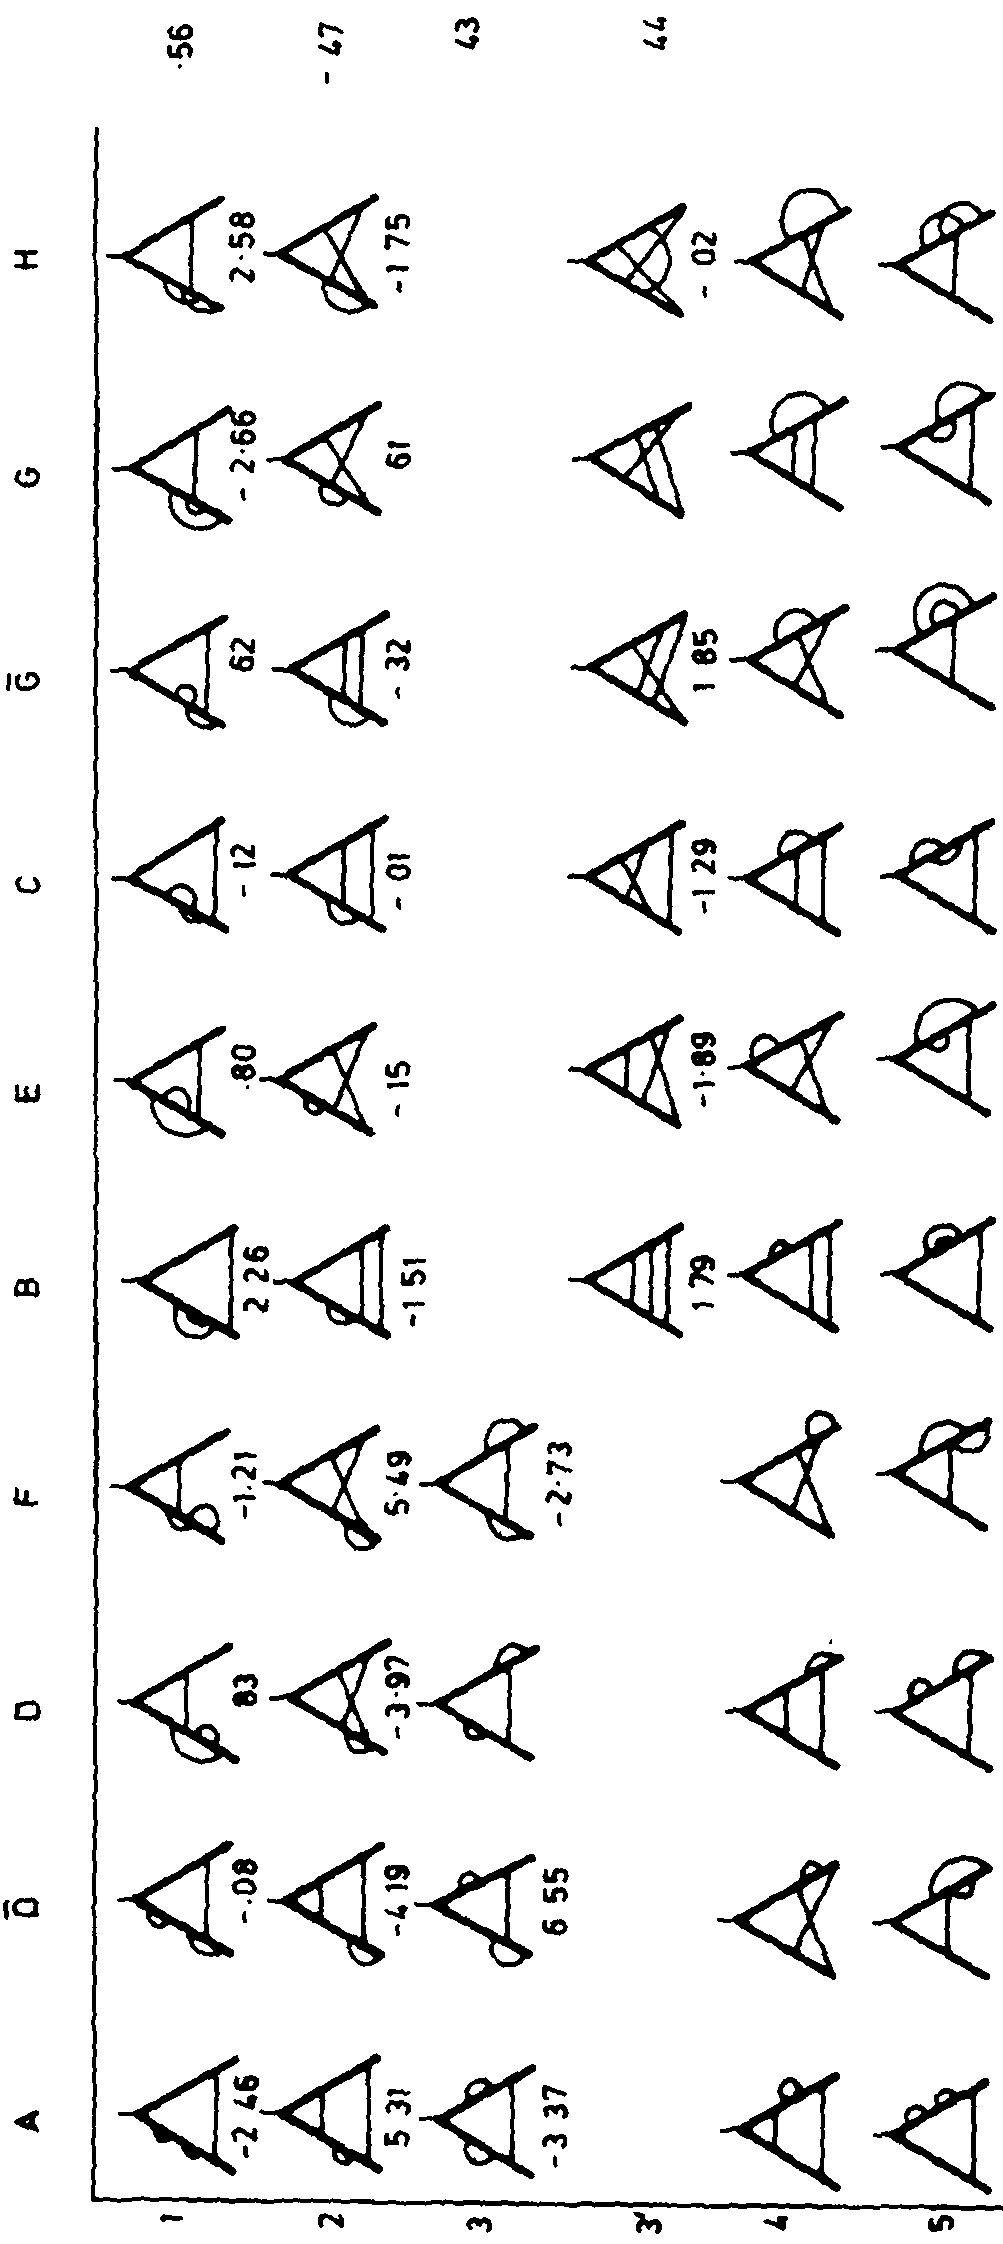
\includegraphics[width=0.44\textwidth,angle=-90]{Cvit77bFig2}
%\end{center}
        } %end \center{
\caption{\label{Cvit77bFig2}
Every vertex diagram belongs both to a `gauge set' and to a `self-energy set'.
This table illustrates the two kinds of sets.
The 3-loop gauge sets $km'm$ are arranged in the rows, and the
self-energy sets (or the `externally gauge-invariant' sets, vertex diagrams
obtained by inserting an extra vertex into a self-energy diagram) in the
columns, labeled as in Fig.~3 of \refref{CviKin74c}. The values are
finite parts in the $\ln\lambda$ IR cut-off approach, such as those
listed in \refref{LevWri73}. For different IR separation methods (such as
in \refref{CviKin74c}) and different gauges, individual diagrams have
different values. The gauge sets, however, are separately gauge invariant.
The self-energy sets (whose number grows combinatorially with the order
in perturbation theory) are not, only their sum is gauge invariant.
From \refref{Cvit77b}.
}
 \end{sidewaysfigure}
%%%%%%%%%%%%%%%%%%%%%%%%%%%%%%%%%%%%%%%%

%%%%%%%%%%%%%%%%%%%%%%%%%%%%%%%%%%%%%%%%
\begin{figure}
\begin{center}
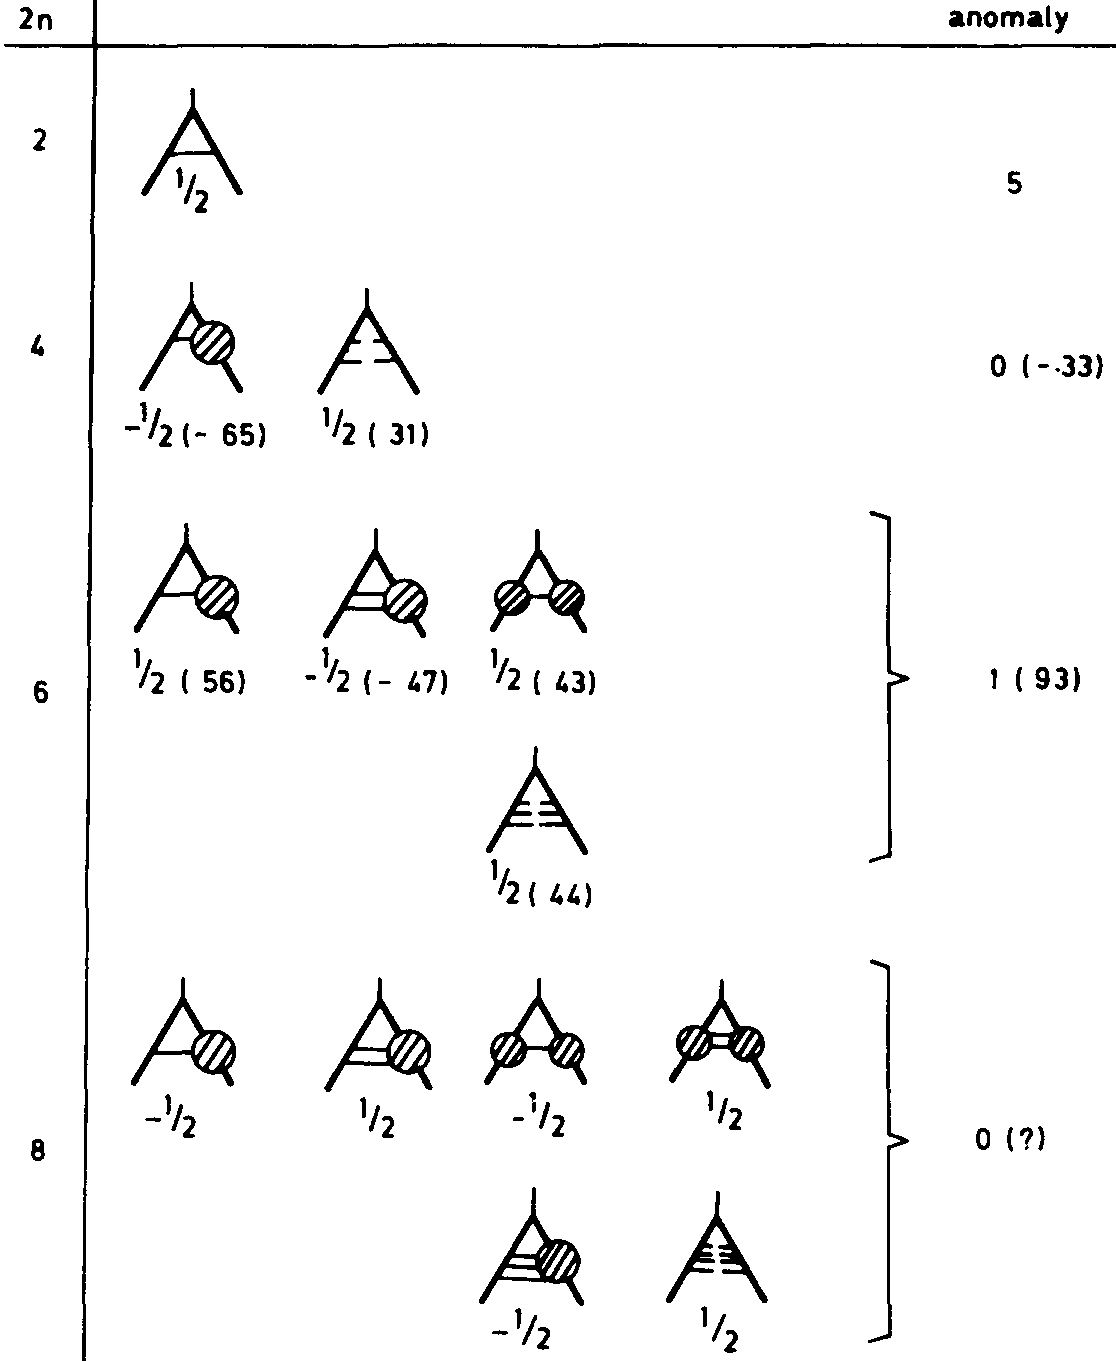
\includegraphics[width=0.90\textwidth]{Cvit77bFig3}
\end{center}
\caption{\label{Cvit77bFig3}
Comparison of the 1977 gauge-set approximation to the anomaly $a$
and the actual numerical
values of corresponding gauge sets, together with the  1977 eighth-order
prediction of \refref{Cvit77b}. For the updated listing, see
\reftab{tabGaugeSets}.
}
 \end{figure}
%%%%%%%%%%%%%%%%%%%%%%%%%%%%%%%%%%%%%%%%

%%%%%%%%%%%%%%%%%%%%%%%%%%%%%%%%%%%%%%%%%%
%%%%%%%%%%%%%%%%%%%%%%%%%%%%%%%%%%%%%%%%%%%%%%%%%%%%%
% tabGaugeSets.tex    2017-06-02
% compiled by  reducesymm/QFT/blog.tex
% needs \usepackage{booktabs}\usepackage{amsmath}
\begin{table}
\centering
{\small
\begin{tabular}{r@{~~~~}ccccc@{~~~~}l}
$2n$ & \multicolumn{5}{c}{$(k,m,m')$} & anomaly \\
    \toprule[1.5pt]\\[-1.0em]
% Entering  row 2
 & $\bf (1,0,0)$
 \\[-1ex]
\raisebox{1.5ex}{2}
 & $\frac{1}{2}$            &&&&& \raisebox{1.5ex}{$\frac{1}{2}$}
  \\[1ex]
 \cmidrule(lr){2-3}\\[-0.8em]
% Entering  row 4
 & $\bf (1,1,0)$  &  $\bf (2,0,0)$
 \\[-1ex]
\raisebox{1.5ex}{4}
 & -$\frac{1}{2}$ (-.65)&  $\frac{1}{2}$  (.31) &&&& \raisebox{1.5ex}{0 (-.33)}
  \\[1ex]
 \cmidrule(lr){2-4}\\[-0.8em]
% Entering  row 6
 & $\bf (1,2,0)$ & $\bf (2,1,0)$   & $\bf (3,0,0)$
 \\[0.1ex]
 & $\frac{1}{2}$ (.56) & -$\frac{1}{2}$ (-.47) &  $\frac{1}{2}$ (.44)
 \\%[-1ex]
\raisebox{1.5ex}{6}
 & $\bf (1,1,1)$ &&&&&          \raisebox{1.5ex}{1 (.93)}\\
 & $\frac{1}{2}$ (.43)
  \\[1ex]
 \cmidrule(lr){2-5}\\[-0.8em]
% Entering  row 8
 & $\bf (1,3,0)$     & $\bf (2,2,0)$  & $\bf (3,1,0)$  & $\bf (4,0,0)$
 \\[0.1ex]
 &  -$\frac{1}{2}${\color{red}$\cdot$4} (-1.97)
                     & $\frac{1}{2}${\color{red}$\cdot 0$ (-0.14)}
                                      & -$\frac{1}{2}${\color{red}$\cdot$2} (-1.04)
                                                        &  $\frac{1}{2}$ (.51)
 \\%[-1ex]
\raisebox{1.5ex}{8}
 & $\bf (1,2,1)$  & $\bf (2,1,1)$ &&&& \raisebox{1.5ex}{0 (-2.17)}\\
 & -$\frac{1}{2}$ (-.62)    &   $\frac{1}{2}${\color{red}$\cdot$2} (1.08)
  \\[1ex]
 \cmidrule(lr){2-6}
% Entering  row 10
 & $\bf (1,4,0)$ & $\bf (2,3,0)$  & $\bf (3,2,0)$
                                        & $\bf (4,1,0)$
                                            & $\bf (5,0,0)$
 \\[0.1ex]
 &    $\frac{1}{2}${\color{red}$\cdot$12} (6.2)
                 & -$\frac{1}{2}$ (-0.72)   & $\frac{1}{2}$  {\color{red} $\cdot 0$ (-0.40)}
                                        & -$\frac{1}{2}${\color{red}$\cdot$2} (-1.02)
                                             &  $\frac{1}{2}${\color{red}$\cdot$2} (1.09)
 \\%[-1ex]
\raisebox{1.5ex}{10}
 & $\bf (1,3,1)$  & $\bf (2,2,1)$ & $\bf (3,1,1)$ &&&
        \raisebox{1.5ex}{$\frac{3}{2} {\color{red} \cdot 4}\,(6.78)$}\\
 &  $\frac{1}{2}$ (0.90)    & -$\frac{1}{2}${\color{red}$\cdot$4} (-2.16)
                                  & $\frac{1}{2}${\color{red}$\cdot$5} (2.62)
  \\[1ex]
 & $\bf (1,2,2)$ \\
 & $\frac{1}{2}$ (0.30)
  \\[1ex]
\bottomrule
\end{tabular}
} %end {\small
\caption{\label{tabGaugeSets}
% Updated \reffig{Cvit77bFig3} comparison of
Comparison of the $\pm\frac{1}{2}$ gauge-set $(k,m,m')$ ansatz \refeq{Cvit77b(5)}
with the actual numerical value of corresponding gauge set, stated in $(\cdots)$
bracket.
Starting with 4-loops, the gauge-set ansatz \refeq{Cvit77b(5)} fails, but in
suggestive ways.
All gauge sets are surprisingly close to integer multiples of 1/2;
the ones differing from multiple 1 are marked in red.
The sign predictions are correct, except for the two anomalously small gauge sets
$(2,2,0)$, and its ``descendent'' $(3,2,0)$.
}
\end{table}
%%%%%%%%%%%%%%%%%%%%%%%%%%%%%%%%%%%%%%%%%%%%%%%%%%%%%

%%%%%%%%%%%%%%%%%%%%%%%%%%%%%%%%%%%%%%%%%%


%%%%%%%%%%%%%%%%%%%%%%%%%%%%%%%%%%%%%%%%%%
%% Laporta17figuragauShort.tex %%%%%
%% compiled by  reducesymm/QFT/blog.tex
%%%%%%%%%%%%%%%%%%%%%%%%%%%%%%%%%%%%%%%%
\begin{figure}[t]
\begin{center}
\begin{picture}(125,50)(70,350)
%\begin{picture}(125,30)(70,350)
\thicklines
%%%
{
\put(+000.0,+200.0){\makebox(0,0)[lb]{
% fotone obliquo (0.000000,200.000000) (0.000000,205.000000)
   \qbezier(+000.0,+200.0)(+001.2,+201.2)(+000.0,+202.5)
   \qbezier(+000.0,+202.5)(-001.2,+203.8)(+000.0,+205.0)
% elettrone curvo (0.000000,200.000000) (-20.000000,160.000000) 1000.000000
% cerchio r=44721.365140 c=(-40010.000000,20180.000000) ang=(-26.536403,-26.593699)
   \qbezier(+000.0,+200.0)(-010.0,+180.0)(-020.0,+160.0)
% elettrone curvo (0.000000,200.000000) (20.000000,160.000000) 1000.000000
% cerchio r=44721.365140 c=(-39990.000000,-19820.000000) ang=(26.593699,26.536403)
   \qbezier(+000.0,+200.0)(+010.0,+180.0)(+020.0,+160.0)
% fotone obliquo (-14.142136,171.715729) (14.142136,171.715729)
   \qbezier(-014.1,+171.7)(-013.3,+170.8)(-012.4,+171.7)
   \qbezier(-012.4,+171.7)(-011.5,+172.6)(-010.6,+171.7)
   \qbezier(-010.6,+171.7)(-009.7,+170.8)(-008.8,+171.7)
   \qbezier(-008.8,+171.7)(-008.0,+172.6)(-007.1,+171.7)
   \qbezier(-007.1,+171.7)(-006.2,+170.8)(-005.3,+171.7)
   \qbezier(-005.3,+171.7)(-004.4,+172.6)(-003.5,+171.7)
   \qbezier(-003.5,+171.7)(-002.7,+170.8)(-001.8,+171.7)
   \qbezier(-001.8,+171.7)(-000.9,+172.6)(+000.0,+171.7)
   \qbezier(+000.0,+171.7)(+000.9,+170.8)(+001.8,+171.7)
   \qbezier(+001.8,+171.7)(+002.7,+172.6)(+003.5,+171.7)
   \qbezier(+003.5,+171.7)(+004.4,+170.8)(+005.3,+171.7)
   \qbezier(+005.3,+171.7)(+006.2,+172.6)(+007.1,+171.7)
   \qbezier(+007.1,+171.7)(+008.0,+170.8)(+008.8,+171.7)
   \qbezier(+008.8,+171.7)(+009.7,+172.6)(+010.6,+171.7)
   \qbezier(+010.6,+171.7)(+011.5,+170.8)(+012.4,+171.7)
   \qbezier(+012.4,+171.7)(+013.3,+172.6)(+014.1,+171.7)
% fotone curvo (5.303301,189.393398) (10.000000,180.000000) 0.100000
% fotone semicircolare r=5.355061 c=(6.712311,184.227029) ang=(105.255119,-52.125016)
% n=8
   \qbezier(+005.3,+189.4)(+006.3,+188.7)(+007.1,+189.6)
   \qbezier(+007.1,+189.6)(+008.3,+190.3)(+008.9,+189.1)
   \qbezier(+008.9,+189.1)(+009.2,+187.9)(+010.4,+188.1)
   \qbezier(+010.4,+188.1)(+011.7,+187.9)(+011.5,+186.6)
   \qbezier(+011.5,+186.6)(+011.0,+185.5)(+012.0,+184.9)
   \qbezier(+012.0,+184.9)(+013.0,+183.9)(+011.9,+183.0)
   \qbezier(+011.9,+183.0)(+010.8,+182.5)(+011.2,+181.4)
   \qbezier(+011.2,+181.4)(+011.3,+180.0)(+010.0,+180.0)
% fotone curvo (12.247449,175.505103) (17.320508,165.358984) 0.100000
% fotone semicircolare r=5.784178 c=(13.769367,169.924737) ang=(105.255119,-52.125016)
% n=9
   \qbezier(+012.2,+175.5)(+013.2,+174.8)(+014.0,+175.7)
   \qbezier(+014.0,+175.7)(+015.0,+176.5)(+015.7,+175.4)
   \qbezier(+015.7,+175.4)(+016.1,+174.2)(+017.3,+174.5)
   \qbezier(+017.3,+174.5)(+018.6,+174.6)(+018.5,+173.3)
   \qbezier(+018.5,+173.3)(+018.2,+172.1)(+019.3,+171.7)
   \qbezier(+019.3,+171.7)(+020.3,+171.0)(+019.6,+170.0)
   \qbezier(+019.6,+170.0)(+018.6,+169.2)(+019.3,+168.2)
   \qbezier(+019.3,+168.2)(+019.8,+167.0)(+018.5,+166.6)
   \qbezier(+018.5,+166.6)(+017.3,+166.5)(+017.3,+165.4)
% fotone curvo (15.811388,168.377223) (18.708287,162.583426) -0.100000
% fotone semicircolare r=3.302973 c=(17.839217,165.770015) ang=(127.874984,285.255119)
% n=5
   \qbezier(+015.8,+168.4)(+014.5,+168.2)(+014.7,+166.9)
   \qbezier(+014.7,+166.9)(+015.4,+166.0)(+014.6,+165.1)
   \qbezier(+014.6,+165.1)(+014.1,+163.9)(+015.4,+163.5)
   \qbezier(+015.4,+163.5)(+016.5,+163.7)(+016.9,+162.6)
   \qbezier(+016.9,+162.6)(+017.8,+161.6)(+018.7,+162.6)
\put(+000.0,+152.0){\makebox(0,0){$(1)$}}
}}
\put(+025.0,+200.0){\makebox(0,0)[lb]{
% fotone obliquo (25.000000,200.000000) (25.000000,205.000000)
   \qbezier(+025.0,+200.0)(+026.2,+201.2)(+025.0,+202.5)
   \qbezier(+025.0,+202.5)(+023.8,+203.8)(+025.0,+205.0)
% elettrone curvo (25.000000,200.000000) (5.000000,160.000000) 1000.000000
% cerchio r=44721.365140 c=(-39985.000000,20180.000000) ang=(-26.536403,-26.593699)
   \qbezier(+025.0,+200.0)(+015.0,+180.0)(+005.0,+160.0)
% elettrone curvo (25.000000,200.000000) (45.000000,160.000000) 1000.000000
% cerchio r=44721.365140 c=(-39965.000000,-19820.000000) ang=(26.593699,26.536403)
   \qbezier(+025.0,+200.0)(+035.0,+180.0)(+045.0,+160.0)
% fotone obliquo (14.309550,178.619101) (35.690450,178.619101)
   \qbezier(+014.3,+178.6)(+015.2,+177.7)(+016.1,+178.6)
   \qbezier(+016.1,+178.6)(+017.0,+179.5)(+017.9,+178.6)
   \qbezier(+017.9,+178.6)(+018.8,+177.7)(+019.7,+178.6)
   \qbezier(+019.7,+178.6)(+020.5,+179.5)(+021.4,+178.6)
   \qbezier(+021.4,+178.6)(+022.3,+177.7)(+023.2,+178.6)
   \qbezier(+023.2,+178.6)(+024.1,+179.5)(+025.0,+178.6)
   \qbezier(+025.0,+178.6)(+025.9,+177.7)(+026.8,+178.6)
   \qbezier(+026.8,+178.6)(+027.7,+179.5)(+028.6,+178.6)
   \qbezier(+028.6,+178.6)(+029.5,+177.7)(+030.3,+178.6)
   \qbezier(+030.3,+178.6)(+031.2,+179.5)(+032.1,+178.6)
   \qbezier(+032.1,+178.6)(+033.0,+177.7)(+033.9,+178.6)
   \qbezier(+033.9,+178.6)(+034.8,+179.5)(+035.7,+178.6)
% fotone obliquo (8.096915,166.193830) (41.903085,166.193830)
   \qbezier(+008.1,+166.2)(+009.0,+165.3)(+009.9,+166.2)
   \qbezier(+009.9,+166.2)(+010.8,+167.1)(+011.7,+166.2)
   \qbezier(+011.7,+166.2)(+012.5,+165.3)(+013.4,+166.2)
   \qbezier(+013.4,+166.2)(+014.3,+167.1)(+015.2,+166.2)
   \qbezier(+015.2,+166.2)(+016.1,+165.3)(+017.0,+166.2)
   \qbezier(+017.0,+166.2)(+017.9,+167.1)(+018.8,+166.2)
   \qbezier(+018.8,+166.2)(+019.7,+165.3)(+020.6,+166.2)
   \qbezier(+020.6,+166.2)(+021.4,+167.1)(+022.3,+166.2)
   \qbezier(+022.3,+166.2)(+023.2,+165.3)(+024.1,+166.2)
   \qbezier(+024.1,+166.2)(+025.0,+167.1)(+025.9,+166.2)
   \qbezier(+025.9,+166.2)(+026.8,+165.3)(+027.7,+166.2)
   \qbezier(+027.7,+166.2)(+028.6,+167.1)(+029.4,+166.2)
   \qbezier(+029.4,+166.2)(+030.3,+165.3)(+031.2,+166.2)
   \qbezier(+031.2,+166.2)(+032.1,+167.1)(+033.0,+166.2)
   \qbezier(+033.0,+166.2)(+033.9,+165.3)(+034.8,+166.2)
   \qbezier(+034.8,+166.2)(+035.7,+167.1)(+036.6,+166.2)
   \qbezier(+036.6,+166.2)(+037.5,+165.3)(+038.3,+166.2)
   \qbezier(+038.3,+166.2)(+039.2,+167.1)(+040.1,+166.2)
   \qbezier(+040.1,+166.2)(+041.0,+165.3)(+041.9,+166.2)
% fotone curvo (32.559289,184.881421) (38.093073,173.813853) 0.100000
% fotone semicircolare r=6.309484 c=(34.219425,178.794259) ang=(105.255119,-52.125016)
% n=9
   \qbezier(+032.6,+184.9)(+033.6,+184.1)(+034.5,+185.1)
   \qbezier(+034.5,+185.1)(+035.6,+185.9)(+036.3,+184.7)
   \qbezier(+036.3,+184.7)(+036.8,+183.5)(+038.0,+183.8)
   \qbezier(+038.0,+183.8)(+039.4,+183.8)(+039.4,+182.4)
   \qbezier(+039.4,+182.4)(+039.0,+181.2)(+040.2,+180.7)
   \qbezier(+040.2,+180.7)(+041.4,+179.9)(+040.5,+178.8)
   \qbezier(+040.5,+178.8)(+039.5,+178.0)(+040.2,+176.9)
   \qbezier(+040.2,+176.9)(+040.7,+175.6)(+039.4,+175.2)
   \qbezier(+039.4,+175.2)(+038.1,+175.1)(+038.1,+173.8)
% fotone curvo (40.118579,169.762842) (43.516402,162.967196) 0.100000
% fotone semicircolare r=3.874114 c=(41.137926,166.025237) ang=(105.255119,-52.125016)
% n=6
   \qbezier(+040.1,+169.8)(+041.0,+169.0)(+041.9,+169.8)
   \qbezier(+041.9,+169.8)(+043.1,+170.3)(+043.5,+169.1)
   \qbezier(+043.5,+169.1)(+043.5,+168.0)(+044.6,+167.8)
   \qbezier(+044.6,+167.8)(+045.7,+167.1)(+045.0,+166.0)
   \qbezier(+045.0,+166.0)(+044.1,+165.4)(+044.6,+164.3)
   \qbezier(+044.6,+164.3)(+044.8,+163.0)(+043.5,+163.0)
\put(+025.0,+152.0){\makebox(0,0){$(2)$}}
}}
\put(+050.0,+200.0){\makebox(0,0)[lb]{
% fotone obliquo (50.000000,200.000000) (50.000000,205.000000)
   \qbezier(+050.0,+200.0)(+051.2,+201.2)(+050.0,+202.5)
   \qbezier(+050.0,+202.5)(+048.8,+203.8)(+050.0,+205.0)
% elettrone curvo (50.000000,200.000000) (30.000000,160.000000) 1000.000000
% cerchio r=44721.365140 c=(-39960.000000,20180.000000) ang=(-26.536403,-26.593699)
   \qbezier(+050.0,+200.0)(+040.0,+180.0)(+030.0,+160.0)
% elettrone curvo (50.000000,200.000000) (70.000000,160.000000) 1000.000000
% cerchio r=44721.365140 c=(-39940.000000,-19820.000000) ang=(26.593699,26.536403)
   \qbezier(+050.0,+200.0)(+060.0,+180.0)(+070.0,+160.0)
% fotone obliquo (33.670068,167.340137) (66.329932,167.340137)
   \qbezier(+033.7,+167.3)(+034.5,+166.5)(+035.4,+167.3)
   \qbezier(+035.4,+167.3)(+036.2,+168.2)(+037.1,+167.3)
   \qbezier(+037.1,+167.3)(+038.0,+166.5)(+038.8,+167.3)
   \qbezier(+038.8,+167.3)(+039.7,+168.2)(+040.5,+167.3)
   \qbezier(+040.5,+167.3)(+041.4,+166.5)(+042.3,+167.3)
   \qbezier(+042.3,+167.3)(+043.1,+168.2)(+044.0,+167.3)
   \qbezier(+044.0,+167.3)(+044.8,+166.5)(+045.7,+167.3)
   \qbezier(+045.7,+167.3)(+046.6,+168.2)(+047.4,+167.3)
   \qbezier(+047.4,+167.3)(+048.3,+166.5)(+049.1,+167.3)
   \qbezier(+049.1,+167.3)(+050.0,+168.2)(+050.9,+167.3)
   \qbezier(+050.9,+167.3)(+051.7,+166.5)(+052.6,+167.3)
   \qbezier(+052.6,+167.3)(+053.4,+168.2)(+054.3,+167.3)
   \qbezier(+054.3,+167.3)(+055.2,+166.5)(+056.0,+167.3)
   \qbezier(+056.0,+167.3)(+056.9,+168.2)(+057.7,+167.3)
   \qbezier(+057.7,+167.3)(+058.6,+166.5)(+059.5,+167.3)
   \qbezier(+059.5,+167.3)(+060.3,+168.2)(+061.2,+167.3)
   \qbezier(+061.2,+167.3)(+062.0,+166.5)(+062.9,+167.3)
   \qbezier(+062.9,+167.3)(+063.8,+168.2)(+064.6,+167.3)
   \qbezier(+064.6,+167.3)(+065.5,+166.5)(+066.3,+167.3)
% fotone curvo (35.857864,171.715729) (31.742581,163.485163) -0.100000
% fotone semicircolare r=4.692144 c=(34.623279,167.188917) ang=(74.744881,232.125016)
% n=7
   \qbezier(+035.9,+171.7)(+035.0,+172.8)(+034.0,+171.8)
   \qbezier(+034.0,+171.8)(+033.4,+170.8)(+032.3,+171.3)
   \qbezier(+032.3,+171.3)(+031.0,+171.4)(+030.9,+170.1)
   \qbezier(+030.9,+170.1)(+031.2,+168.9)(+030.1,+168.4)
   \qbezier(+030.1,+168.4)(+029.0,+167.6)(+030.0,+166.6)
   \qbezier(+030.0,+166.6)(+031.0,+166.0)(+030.5,+164.9)
   \qbezier(+030.5,+164.9)(+030.4,+163.5)(+031.7,+163.5)
% fotone curvo (64.142136,171.715729) (68.257419,163.485163) 0.100000
% fotone semicircolare r=4.692144 c=(65.376721,167.188917) ang=(105.255119,-52.125016)
% n=7
   \qbezier(+064.1,+171.7)(+065.1,+171.0)(+066.0,+171.8)
   \qbezier(+066.0,+171.8)(+067.1,+172.5)(+067.7,+171.3)
   \qbezier(+067.7,+171.3)(+067.9,+170.1)(+069.1,+170.1)
   \qbezier(+069.1,+170.1)(+070.4,+169.7)(+069.9,+168.4)
   \qbezier(+069.9,+168.4)(+069.2,+167.5)(+070.0,+166.6)
   \qbezier(+070.0,+166.6)(+070.7,+165.4)(+069.5,+164.9)
   \qbezier(+069.5,+164.9)(+068.2,+164.7)(+068.3,+163.5)
% fotone curvo (56.123724,187.752551) (61.547005,176.905989) 0.100000
% fotone semicircolare r=6.183492 c=(57.750709,181.786942) ang=(105.255119,-52.125016)
% n=9
   \qbezier(+056.1,+187.8)(+057.2,+187.0)(+058.0,+188.0)
   \qbezier(+058.0,+188.0)(+059.1,+188.8)(+059.8,+187.6)
   \qbezier(+059.8,+187.6)(+060.3,+186.4)(+061.5,+186.7)
   \qbezier(+061.5,+186.7)(+062.9,+186.7)(+062.8,+185.4)
   \qbezier(+062.8,+185.4)(+062.5,+184.1)(+063.6,+183.7)
   \qbezier(+063.6,+183.7)(+064.8,+182.9)(+063.9,+181.8)
   \qbezier(+063.9,+181.8)(+062.9,+181.0)(+063.7,+180.0)
   \qbezier(+063.7,+180.0)(+064.1,+178.7)(+062.8,+178.3)
   \qbezier(+062.8,+178.3)(+061.6,+178.2)(+061.5,+176.9)
\put(+050.0,+152.0){\makebox(0,0){$(3)$}}
}}
\put(+075.0,+200.0){\makebox(0,0)[lb]{
% fotone obliquo (75.000000,200.000000) (75.000000,205.000000)
   \qbezier(+075.0,+200.0)(+076.2,+201.2)(+075.0,+202.5)
   \qbezier(+075.0,+202.5)(+073.8,+203.8)(+075.0,+205.0)
% elettrone curvo (75.000000,200.000000) (55.000000,160.000000) 1000.000000
% cerchio r=44721.365140 c=(-39935.000000,20180.000000) ang=(-26.536403,-26.593699)
   \qbezier(+075.0,+200.0)(+065.0,+180.0)(+055.0,+160.0)
% elettrone curvo (75.000000,200.000000) (95.000000,160.000000) 1000.000000
% cerchio r=44721.365140 c=(-39915.000000,-19820.000000) ang=(26.593699,26.536403)
   \qbezier(+075.0,+200.0)(+085.0,+180.0)(+095.0,+160.0)
% fotone obliquo (66.835034,183.670068) (91.329932,167.340137)
   \qbezier(+066.8,+183.7)(+067.1,+182.5)(+068.3,+182.7)
   \qbezier(+068.3,+182.7)(+069.5,+182.9)(+069.7,+181.7)
   \qbezier(+069.7,+181.7)(+070.0,+180.5)(+071.2,+180.8)
   \qbezier(+071.2,+180.8)(+072.4,+181.0)(+072.6,+179.8)
   \qbezier(+072.6,+179.8)(+072.8,+178.6)(+074.0,+178.9)
   \qbezier(+074.0,+178.9)(+075.2,+179.1)(+075.5,+177.9)
   \qbezier(+075.5,+177.9)(+075.7,+176.7)(+076.9,+176.9)
   \qbezier(+076.9,+176.9)(+078.1,+177.2)(+078.4,+176.0)
   \qbezier(+078.4,+176.0)(+078.6,+174.8)(+079.8,+175.0)
   \qbezier(+079.8,+175.0)(+081.0,+175.3)(+081.2,+174.1)
   \qbezier(+081.2,+174.1)(+081.5,+172.9)(+082.7,+173.1)
   \qbezier(+082.7,+173.1)(+083.9,+173.3)(+084.1,+172.1)
   \qbezier(+084.1,+172.1)(+084.4,+170.9)(+085.6,+171.2)
   \qbezier(+085.6,+171.2)(+086.8,+171.4)(+087.0,+170.2)
   \qbezier(+087.0,+170.2)(+087.2,+169.0)(+088.4,+169.3)
   \qbezier(+088.4,+169.3)(+089.6,+169.5)(+089.9,+168.3)
   \qbezier(+089.9,+168.3)(+090.1,+167.1)(+091.3,+167.3)
% fotone obliquo (58.670068,167.340137) (83.164966,183.670068)
   \qbezier(+058.7,+167.3)(+059.9,+167.1)(+060.1,+168.3)
   \qbezier(+060.1,+168.3)(+060.4,+169.5)(+061.6,+169.3)
   \qbezier(+061.6,+169.3)(+062.8,+169.0)(+063.0,+170.2)
   \qbezier(+063.0,+170.2)(+063.2,+171.4)(+064.4,+171.2)
   \qbezier(+064.4,+171.2)(+065.6,+170.9)(+065.9,+172.1)
   \qbezier(+065.9,+172.1)(+066.1,+173.3)(+067.3,+173.1)
   \qbezier(+067.3,+173.1)(+068.5,+172.9)(+068.8,+174.1)
   \qbezier(+068.8,+174.1)(+069.0,+175.3)(+070.2,+175.0)
   \qbezier(+070.2,+175.0)(+071.4,+174.8)(+071.6,+176.0)
   \qbezier(+071.6,+176.0)(+071.9,+177.2)(+073.1,+176.9)
   \qbezier(+073.1,+176.9)(+074.3,+176.7)(+074.5,+177.9)
   \qbezier(+074.5,+177.9)(+074.8,+179.1)(+076.0,+178.9)
   \qbezier(+076.0,+178.9)(+077.2,+178.6)(+077.4,+179.8)
   \qbezier(+077.4,+179.8)(+077.6,+181.0)(+078.8,+180.8)
   \qbezier(+078.8,+180.8)(+080.0,+180.5)(+080.3,+181.7)
   \qbezier(+080.3,+181.7)(+080.5,+182.9)(+081.7,+182.7)
   \qbezier(+081.7,+182.7)(+082.9,+182.5)(+083.2,+183.7)
% fotone curvo (60.857864,171.715729) (56.742581,163.485163) -0.100000
% fotone semicircolare r=4.692144 c=(59.623279,167.188917) ang=(74.744881,232.125016)
% n=7
   \qbezier(+060.9,+171.7)(+060.0,+172.8)(+059.0,+171.8)
   \qbezier(+059.0,+171.8)(+058.4,+170.8)(+057.3,+171.3)
   \qbezier(+057.3,+171.3)(+056.0,+171.4)(+055.9,+170.1)
   \qbezier(+055.9,+170.1)(+056.2,+168.9)(+055.1,+168.4)
   \qbezier(+055.1,+168.4)(+054.0,+167.6)(+055.0,+166.6)
   \qbezier(+055.0,+166.6)(+056.0,+166.0)(+055.5,+164.9)
   \qbezier(+055.5,+164.9)(+055.4,+163.5)(+056.7,+163.5)
% fotone curvo (85.526385,178.947231) (89.142136,171.715729) 0.100000
% fotone semicircolare r=4.122590 c=(86.611110,174.969905) ang=(105.255119,-52.125016)
% n=6
   \qbezier(+085.5,+178.9)(+086.5,+178.2)(+087.4,+179.0)
   \qbezier(+087.4,+179.0)(+088.7,+179.6)(+089.1,+178.3)
   \qbezier(+089.1,+178.3)(+089.1,+177.0)(+090.3,+176.8)
   \qbezier(+090.3,+176.8)(+091.5,+176.1)(+090.7,+175.0)
   \qbezier(+090.7,+175.0)(+089.7,+174.3)(+090.3,+173.2)
   \qbezier(+090.3,+173.2)(+090.5,+171.8)(+089.1,+171.7)
\put(+075.0,+152.0){\makebox(0,0){$(4)$}}
}}
\put(+100.0,+200.0){\makebox(0,0)[lb]{
% fotone obliquo (100.000000,200.000000) (100.000000,205.000000)
   \qbezier(+100.0,+200.0)(+101.2,+201.2)(+100.0,+202.5)
   \qbezier(+100.0,+202.5)(+098.8,+203.8)(+100.0,+205.0)
% elettrone curvo (100.000000,200.000000) (80.000000,160.000000) 1000.000000
% cerchio r=44721.365140 c=(-39910.000000,20180.000000) ang=(-26.536403,-26.593699)
   \qbezier(+100.0,+200.0)(+090.0,+180.0)(+080.0,+160.0)
% elettrone curvo (100.000000,200.000000) (120.000000,160.000000) 1000.000000
% cerchio r=44721.365140 c=(-39890.000000,-19820.000000) ang=(26.593699,26.536403)
   \qbezier(+100.0,+200.0)(+110.0,+180.0)(+120.0,+160.0)
% fotone obliquo (91.835034,183.670068) (114.142136,171.715729)
   \qbezier(+091.8,+183.7)(+092.2,+182.4)(+093.4,+182.8)
   \qbezier(+093.4,+182.8)(+094.7,+183.2)(+095.0,+182.0)
   \qbezier(+095.0,+182.0)(+095.4,+180.7)(+096.6,+181.1)
   \qbezier(+096.6,+181.1)(+097.8,+181.5)(+098.2,+180.3)
   \qbezier(+098.2,+180.3)(+098.6,+179.0)(+099.8,+179.4)
   \qbezier(+099.8,+179.4)(+101.0,+179.8)(+101.4,+178.5)
   \qbezier(+101.4,+178.5)(+101.8,+177.3)(+103.0,+177.7)
   \qbezier(+103.0,+177.7)(+104.2,+178.1)(+104.6,+176.8)
   \qbezier(+104.6,+176.8)(+105.0,+175.6)(+106.2,+176.0)
   \qbezier(+106.2,+176.0)(+107.4,+176.4)(+107.8,+175.1)
   \qbezier(+107.8,+175.1)(+108.1,+173.9)(+109.4,+174.3)
   \qbezier(+109.4,+174.3)(+110.6,+174.6)(+111.0,+173.4)
   \qbezier(+111.0,+173.4)(+111.3,+172.2)(+112.5,+172.6)
   \qbezier(+112.5,+172.6)(+113.8,+172.9)(+114.1,+171.7)
% fotone obliquo (85.857864,171.715729) (108.164966,183.670068)
   \qbezier(+085.9,+171.7)(+087.1,+171.3)(+087.5,+172.6)
   \qbezier(+087.5,+172.6)(+087.8,+173.8)(+089.0,+173.4)
   \qbezier(+089.0,+173.4)(+090.3,+173.1)(+090.6,+174.3)
   \qbezier(+090.6,+174.3)(+091.0,+175.5)(+092.2,+175.1)
   \qbezier(+092.2,+175.1)(+093.5,+174.8)(+093.8,+176.0)
   \qbezier(+093.8,+176.0)(+094.2,+177.2)(+095.4,+176.8)
   \qbezier(+095.4,+176.8)(+096.6,+176.5)(+097.0,+177.7)
   \qbezier(+097.0,+177.7)(+097.4,+178.9)(+098.6,+178.5)
   \qbezier(+098.6,+178.5)(+099.8,+178.2)(+100.2,+179.4)
   \qbezier(+100.2,+179.4)(+100.6,+180.6)(+101.8,+180.3)
   \qbezier(+101.8,+180.3)(+103.0,+179.9)(+103.4,+181.1)
   \qbezier(+103.4,+181.1)(+103.8,+182.3)(+105.0,+182.0)
   \qbezier(+105.0,+182.0)(+106.2,+181.6)(+106.6,+182.8)
   \qbezier(+106.6,+182.8)(+106.9,+184.0)(+108.2,+183.7)
% fotone obliquo (81.742581,163.485163) (118.257419,163.485163)
   \qbezier(+081.7,+163.5)(+082.6,+162.6)(+083.5,+163.5)
   \qbezier(+083.5,+163.5)(+084.4,+164.4)(+085.2,+163.5)
   \qbezier(+085.2,+163.5)(+086.1,+162.6)(+087.0,+163.5)
   \qbezier(+087.0,+163.5)(+087.8,+164.4)(+088.7,+163.5)
   \qbezier(+088.7,+163.5)(+089.6,+162.6)(+090.4,+163.5)
   \qbezier(+090.4,+163.5)(+091.3,+164.4)(+092.2,+163.5)
   \qbezier(+092.2,+163.5)(+093.0,+162.6)(+093.9,+163.5)
   \qbezier(+093.9,+163.5)(+094.8,+164.4)(+095.7,+163.5)
   \qbezier(+095.7,+163.5)(+096.5,+162.6)(+097.4,+163.5)
   \qbezier(+097.4,+163.5)(+098.3,+164.4)(+099.1,+163.5)
   \qbezier(+099.1,+163.5)(+100.0,+162.6)(+100.9,+163.5)
   \qbezier(+100.9,+163.5)(+101.7,+164.4)(+102.6,+163.5)
   \qbezier(+102.6,+163.5)(+103.5,+162.6)(+104.3,+163.5)
   \qbezier(+104.3,+163.5)(+105.2,+164.4)(+106.1,+163.5)
   \qbezier(+106.1,+163.5)(+107.0,+162.6)(+107.8,+163.5)
   \qbezier(+107.8,+163.5)(+108.7,+164.4)(+109.6,+163.5)
   \qbezier(+109.6,+163.5)(+110.4,+162.6)(+111.3,+163.5)
   \qbezier(+111.3,+163.5)(+112.2,+164.4)(+113.0,+163.5)
   \qbezier(+113.0,+163.5)(+113.9,+162.6)(+114.8,+163.5)
   \qbezier(+114.8,+163.5)(+115.6,+164.4)(+116.5,+163.5)
   \qbezier(+116.5,+163.5)(+117.4,+162.6)(+118.3,+163.5)
% fotone curvo (111.547005,176.905989) (116.329932,167.340137) 0.100000
% fotone semicircolare r=5.453375 c=(112.981883,171.644770) ang=(105.255119,-52.125016)
% n=8
   \qbezier(+111.5,+176.9)(+112.6,+176.2)(+113.4,+177.1)
   \qbezier(+113.4,+177.1)(+114.6,+177.8)(+115.2,+176.6)
   \qbezier(+115.2,+176.6)(+115.5,+175.4)(+116.8,+175.6)
   \qbezier(+116.8,+175.6)(+118.1,+175.4)(+117.9,+174.1)
   \qbezier(+117.9,+174.1)(+117.3,+173.0)(+118.4,+172.3)
   \qbezier(+118.4,+172.3)(+119.3,+171.3)(+118.3,+170.4)
   \qbezier(+118.3,+170.4)(+117.2,+169.9)(+117.6,+168.7)
   \qbezier(+117.6,+168.7)(+117.7,+167.4)(+116.3,+167.3)
\put(+100.0,+152.0){\makebox(0,0){$(5)$}}
}}
\put(+250.0,+235.0){\makebox(0,0)[lb]{
% fotone obliquo (0.000000,165.000000) (0.000000,170.000000)
   \qbezier(+000.0,+165.0)(+001.2,+166.2)(+000.0,+167.5)
   \qbezier(+000.0,+167.5)(-001.2,+168.8)(+000.0,+170.0)
% elettrone curvo (0.000000,165.000000) (-20.000000,125.000000) 1000.000000
% cerchio r=44721.365140 c=(-40010.000000,20145.000000) ang=(-26.536403,-26.593699)
   \qbezier(+000.0,+165.0)(-010.0,+145.0)(-020.0,+125.0)
% elettrone curvo (0.000000,165.000000) (20.000000,125.000000) 1000.000000
% cerchio r=44721.365140 c=(-39990.000000,-19855.000000) ang=(26.593699,26.536403)
   \qbezier(+000.0,+165.0)(+010.0,+145.0)(+020.0,+125.0)
% fotone obliquo (-8.944272,147.111456) (12.649111,139.701779)
   \qbezier(-008.9,+147.1)(-008.4,+146.0)(-007.3,+146.5)
   \qbezier(-007.3,+146.5)(-006.2,+147.1)(-005.6,+146.0)
   \qbezier(-005.6,+146.0)(-005.1,+144.9)(-004.0,+145.4)
   \qbezier(-004.0,+145.4)(-002.8,+145.9)(-002.3,+144.8)
   \qbezier(-002.3,+144.8)(-001.8,+143.7)(-000.6,+144.3)
   \qbezier(-000.6,+144.3)(+000.5,+144.8)(+001.0,+143.7)
   \qbezier(+001.0,+143.7)(+001.6,+142.6)(+002.7,+143.1)
   \qbezier(+002.7,+143.1)(+003.8,+143.7)(+004.3,+142.6)
   \qbezier(+004.3,+142.6)(+004.9,+141.4)(+006.0,+142.0)
   \qbezier(+006.0,+142.0)(+007.1,+142.5)(+007.7,+141.4)
   \qbezier(+007.7,+141.4)(+008.2,+140.3)(+009.3,+140.8)
   \qbezier(+009.3,+140.8)(+010.4,+141.4)(+011.0,+140.3)
   \qbezier(+011.0,+140.3)(+011.5,+139.2)(+012.6,+139.7)
% fotone obliquo (-12.649111,139.701779) (15.491933,134.016133)
   \qbezier(-012.6,+139.7)(-011.9,+138.6)(-010.9,+139.3)
   \qbezier(-010.9,+139.3)(-009.8,+140.0)(-009.1,+139.0)
   \qbezier(-009.1,+139.0)(-008.4,+137.9)(-007.4,+138.6)
   \qbezier(-007.4,+138.6)(-006.3,+139.3)(-005.6,+138.3)
   \qbezier(-005.6,+138.3)(-004.9,+137.2)(-003.9,+137.9)
   \qbezier(-003.9,+137.9)(-002.8,+138.6)(-002.1,+137.6)
   \qbezier(-002.1,+137.6)(-001.4,+136.5)(-000.3,+137.2)
   \qbezier(-000.3,+137.2)(+000.7,+137.9)(+001.4,+136.9)
   \qbezier(+001.4,+136.9)(+002.1,+135.8)(+003.2,+136.5)
   \qbezier(+003.2,+136.5)(+004.2,+137.2)(+004.9,+136.1)
   \qbezier(+004.9,+136.1)(+005.6,+135.1)(+006.7,+135.8)
   \qbezier(+006.7,+135.8)(+007.8,+136.5)(+008.5,+135.4)
   \qbezier(+008.5,+135.4)(+009.2,+134.4)(+010.2,+135.1)
   \qbezier(+010.2,+135.1)(+011.3,+135.8)(+012.0,+134.7)
   \qbezier(+012.0,+134.7)(+012.7,+133.7)(+013.7,+134.4)
   \qbezier(+013.7,+134.4)(+014.8,+135.1)(+015.5,+134.0)
% fotone obliquo (-15.491933,134.016133) (17.888544,129.222912)
   \qbezier(-015.5,+134.0)(-014.7,+133.0)(-013.7,+133.8)
   \qbezier(-013.7,+133.8)(-012.7,+134.5)(-012.0,+133.5)
   \qbezier(-012.0,+133.5)(-011.2,+132.5)(-010.2,+133.3)
   \qbezier(-010.2,+133.3)(-009.2,+134.0)(-008.5,+133.0)
   \qbezier(-008.5,+133.0)(-007.7,+132.0)(-006.7,+132.8)
   \qbezier(-006.7,+132.8)(-005.7,+133.5)(-005.0,+132.5)
   \qbezier(-005.0,+132.5)(-004.2,+131.5)(-003.2,+132.3)
   \qbezier(-003.2,+132.3)(-002.2,+133.0)(-001.4,+132.0)
   \qbezier(-001.4,+132.0)(-000.7,+131.0)(+000.3,+131.7)
   \qbezier(+000.3,+131.7)(+001.3,+132.5)(+002.1,+131.5)
   \qbezier(+002.1,+131.5)(+002.8,+130.5)(+003.8,+131.2)
   \qbezier(+003.8,+131.2)(+004.8,+132.0)(+005.6,+131.0)
   \qbezier(+005.6,+131.0)(+006.3,+130.0)(+007.3,+130.7)
   \qbezier(+007.3,+130.7)(+008.4,+131.5)(+009.1,+130.5)
   \qbezier(+009.1,+130.5)(+009.9,+129.5)(+010.9,+130.2)
   \qbezier(+010.9,+130.2)(+011.9,+131.0)(+012.6,+130.0)
   \qbezier(+012.6,+130.0)(+013.4,+129.0)(+014.4,+129.7)
   \qbezier(+014.4,+129.7)(+015.4,+130.5)(+016.1,+129.5)
   \qbezier(+016.1,+129.5)(+016.9,+128.5)(+017.9,+129.2)
% fotone obliquo (-17.888544,129.222912) (8.944272,147.111456)
   \qbezier(-017.9,+129.2)(-016.6,+129.0)(-016.4,+130.2)
   \qbezier(-016.4,+130.2)(-016.1,+131.5)(-014.9,+131.2)
   \qbezier(-014.9,+131.2)(-013.7,+131.0)(-013.4,+132.2)
   \qbezier(-013.4,+132.2)(-013.2,+133.4)(-011.9,+133.2)
   \qbezier(-011.9,+133.2)(-010.7,+132.9)(-010.4,+134.2)
   \qbezier(-010.4,+134.2)(-010.2,+135.4)(-008.9,+135.2)
   \qbezier(-008.9,+135.2)(-007.7,+134.9)(-007.5,+136.2)
   \qbezier(-007.5,+136.2)(-007.2,+137.4)(-006.0,+137.2)
   \qbezier(-006.0,+137.2)(-004.7,+136.9)(-004.5,+138.2)
   \qbezier(-004.5,+138.2)(-004.2,+139.4)(-003.0,+139.2)
   \qbezier(-003.0,+139.2)(-001.7,+138.9)(-001.5,+140.2)
   \qbezier(-001.5,+140.2)(-001.2,+141.4)(-000.0,+141.1)
   \qbezier(+000.0,+141.1)(+001.2,+140.9)(+001.5,+142.1)
   \qbezier(+001.5,+142.1)(+001.7,+143.4)(+003.0,+143.1)
   \qbezier(+003.0,+143.1)(+004.2,+142.9)(+004.5,+144.1)
   \qbezier(+004.5,+144.1)(+004.7,+145.4)(+006.0,+145.1)
   \qbezier(+006.0,+145.1)(+007.2,+144.9)(+007.5,+146.1)
   \qbezier(+007.5,+146.1)(+007.7,+147.4)(+008.9,+147.1)
\put(+000.0,+117.0){\makebox(0,0){$(6)$}}
}}
}
%%%
 \end{picture}
  \\[3ex]
\begin{tabular}{ccrrr}
gauge set &$(k,m,m')$& value~~ & prediction \\
\hline
   (1)  & (1,3,0) & - 1.9710    & - 1/2  \\%01
   (2)  & (2,2,0) &  - 0.1424   & \phantom{+} 1/2 &~(!)\\%02
   (3)  & (1,2,1) &  - 0.6219   & - 1/2  \\%03
   (4)  & (2,1,1) &  \phantom{+} 1.0867  & \phantom{+} 1/2  \\%04
   (5)  & (3,1,0) &  - 1.0405   & - 1/2  \\%05
   (6)  & (4,0,0) &  \phantom{+} 0.5125  & \phantom{+} 1/2  \\%06
\hline
%  1+2+{\ldots}+6 & - 2.176866027739540077443259355895893938670  \\
% -2*1.9710-2*0.14249-2*0.6219+1.0867-2*1.0405+0.5125 =
% -1.9710-0.14249-0.6219+1.0867-1.0405+0.5125 =  -2.17669
\end{tabular}
 \end{center}
%%/ \phantom{ }\vspace{0truecm}\phantom{ }
\caption{\label{Laporta17figuragauShort}
(top)
Examples of 4-loop vertex diagrams belonging to Laporta\rf{Laporta17} gauge sets
(1) to (6).
%(1) = $(1,3,0)$,
%(2) = $(2,2,0)$,
%(3) = $(1,2,1)$,
%(4) = $(2,1,1)$,
%(5) = $(3,1,0)$,
%(6) = $(4,0,0)$.
The remaining diagrams in the set can be obtained by permuting separately
the vertices on the left and right side of the electron line, and
considering also the mirror images of the diagrams. For all 25
gauge-invariant sets, see \reffig{Laporta17figuragau}.
The table:
Gauge-set contributions $a^{(8)}_{kmm'}$, see \refeq{quenchAnom}, as
reported by Laporta\rf{Laporta17}
(for the full 25 gauge-invariant sets, see \reftab{Laporta17:tableset}).
The last column: 1977 Cvitanovi\'c predictions\rf{Cvit77b}.
Signs are right, except for the set (2) = $(2,2,0)$, which is anomalously
small, and the remaining sets are surprisingly close to multiples of 1/2.
There might be factors of 2 having to do with symmetries, missing from
the guesses of \refref{Cvit77b}, but I cannot see how that would work.
Only (4) = $(2,1,1)$ and  (6) = $(4,0,0)$ are symmetric,
but (1) = $(1,3,0)$, (4) and (5) = $(3,1,0)$ seem to
have an extra factor of 2 or 4.
}
 \end{figure}
%%%%%%%%%%%%%%%%%%%%%%%%%%%%%%%%%%%%%%%%

%%%%%%%%%%%%%%%%%%%%%%%%%%%%%%%%%%%%%%%%%%


\subsection{Self-energy sets}
\label{sect:selfEnergy}

There are two ways of grouping vertex diagrams, into \emph{gauge sets},
and into \emph{self-energy sets} (or the ``externally gauge-invariant''
sets). Every vertex diagram belongs both to a gauge set and to a
self-energy set, as illustrated by \reffig{Cvit77bFig2}.
Formulation of the $(g-2)$ computation directly from self-energy graphs
is due to
\HREF{http://chaosbook.org/~predrag/papers/preprints.html\#PerturbativeQED}
{Cvitanovi\'{c} and Kinoshita}, see the ``new formula'' (6.22) in
\refref{CviKin74c}. Not only does this calculation use fewer Feynman
graphs, but it enables calculation of the 3-loop electron magnetic moment
by two independent methods (and in this way helps track down and
eliminate errors in either calculation). As an important aside,
Carroll\rf{CarYao74, Carroll75} gives the credit for self-energy sets
only to the mass-operator formalism of Schwinger\rf{Schwinger51a,
Schwinger51b, Schwinger51c, Sommerfield58}, even though Carroll papers
look closer to \refref{CviKin74c} than to Schwinger and Sommerfield;
\refref{CviKin74c} is cited, and his derivation is also based on the
Ward-Takahashi identity\rf{Ward50,Takahashi57}. The self-energy set
formulation might be equivalent to Schwinger's, but it looks quite
different in detail, and the authors were not aware of Schwinger
mass-operator when they derived it.

The gauge sets are minimal, and separately gauge invariant (for a proof,
see \refref{Cvit77b}). The self-energy sets are not, only their sum is
gauge invariant.
Unlike gauge sets, whose number grows polynomially, the number of
self-energy sets grows combinatorially - they save significant amount
of computing for few-loops computations, but cannot be used to argue the
finiteness of QED.
That is the reason why Aoyama \etal\rf{AoHaKiNi12,AoHaKiNi15,AoKiNi18}
calculations have nothing to say about the 1977 conjecture\rf{Cvit77b}:
they do not compute individual vertex diagrams, but only the self-energy
sets, and for them the set of all diagrams without a fermion loop
(`quenched-' or `q-type' diagrams) is a single `gauge set'
$V$. For example, for 5-loops the set $V$ is a sum of 9 vertex gauge sets
(where time-reversed pairs count as one set, see \reftab{tabGaugeSets}),
but Aoyama \etal\rf{AoKiNi18} only give their sum \refeq{anomalValues}.

\subsection{Where do we go from here?}
\label{sect:future}

\begin{bartlett}{
\HREF{http://chaosbook.org/~predrag/papers/finitness.html}
{Gauge invariance is the bane of my life}
        }
\bauthor{
Predrag
    }
\end{bartlett}
\bigskip

\noindent
Aoyama \etal\ 5-loop calculations already push the envelope of what is
numerically attainable, they cannot switch from the self-energy
diagrams formulation to the vertex diagrams formulation, it would mean
(for the quenched set $V$) going from 389 self-energy graphs to 6354
vertex diagrams. Stefano Laporta deserves a bit of well earned rest. So
what is ahead?

At this time, Sergey  A. Volkov appears to be the
only person set up do the requisite 5-loop calculations,
see \refsect{sect:Volkov}.

Two approaches might be relevant to
establishing bounds on, and perhaps even the direct computation
of gauge sets (ignoring the $N\!=\!2$ and $N\!=\!4$
supersymmetric models):
(1)
\emph{worldline formalism} pursued by
\HREF{http://www.ifm.umich.mx/ifm/index.php/fisca/academicos/schubert/}
{Schubert} and collaborators,
see \refsect{sect:worldline},
and
(2)
\emph{Hopf algebraic approach} of Kreimer and collaborators,
see \refsect{sect:HopfAlgebra}.

Very far out in the left field is the smooth conjugacy method of
\refsect{sect:scfpo} which would require a bit of real work to apply it
to a field theory.

%\section{Worldline formalism}
%\label{sect:worldline}
% reducesymm/QFT/worldline.tex
%%%%%%%%%%%%%%%%%%%%%%%%%%%%%%%%%%%%%%%%%%%%%%%%%%%%%%%%%%%%%%%%%%%%%%%%%

\section{Worldline formalism}
\label{sect:worldline}

How and why Feynman in 1950 introduced `worldline formalism' (initially
for scalar QED, appendix to \refref{Feynman50}, then for spinor QED,
appendix to \refref{Feynman51}) is explained in Schubert 2001
report\rf{Schubert01} (which also has an extensive bibliography up to
2001).
In 1982 Affleck, Alvarez, and Manton\rf{AffAlMa82} used the Feynman
worldline path integral representation of the quenched effective action
for scalar QED in the constant electric field.

For the remainder of this section we shall consider only the quenched
QED, \ie, restrict our considerations only to sets of diagrams with no
lepton loop insertions.

A formula for the charged scalar propagator to emit and reabsorb $N$
photons as it propagates from $x'$ to $x$ can be derived
as follows\rf{AhBaSc16}.
The free scalar propagator for the Euclidean
Klein-Gordon equation\rf{Schubert12,AhBaSc16} is
\beq
D_0(x,x')=\bra{x}\frac{1}{-\Box +m^2}\ket{x'}
\,,
\ee{Schubert12(1.1)}
where $\Box$ is the $D$-dimensional Laplacian. Exponentiate the
denominator following Schwinger,
% proper-time parameter $T$
\beq
D_0(x,x')=\int_0^\infty\!\!dT\,{e}^{-m^2T}\bra{x}e^{-T(-\Box)}\ket{x'}
\,,
\ee{Schubert12(1.4)}
Replace the operator in the exponent by a path integral
\beq
D_0(x,x')=\int_0^\infty\!\!dT\,e^{-m^2T}
\int_{x(0)=x'}^{x(T)=x}\!\!\!\!\mathcal{D}x(\tau)\,
    e^{-\int_0^T\!\!d\tau \frac{1}{4}\dot{x}^2}
\,,
\ee{Schubert12(1.7)}
where $\tau$ is a proper-time parameter (the fifth parameter\rf{Fock37}), and
the dot denotes a derivative with respect to the proper time. This is the
\emph{worldline path integral} representation of the relativistic propagator
of a scalar particle in Euclidean space-time. In the vacuum (no background
field), it is easily evaluated by standard methods and leads to the usual
space and momentum space free propagators,
    \PC{2017-06-17
Here a study of Sect.~6. {\em Worldline formalism} of Gelis and N.
Tanji\rf{GelTan16} might be helpful - it reexpresses the integral as an
average over Wilson loops.
    }
\beq
\int_{x(0)=x'}^{x(T)=x}\!\!\!\!\mathcal{D}x(\tau)\,
    e^{-\int_0^T\!\!d\tau \frac{1}{4}\dot{x}^2}
        =
\frac{1}{(4\pi T)^{d/2}}
\,.
\ee{GelTan16(186)}
Adding the QED
interaction terms leads to the Feynman's worldline path integral
representation\rf{Feynman50} of the charged scalar propagator  of mass
$m$ in the presence of a background field $A(x)$,
\beq
D(x,x')=\int_0^\infty\!\!dT\,e^{-m^2T}
    \int_{x(0)=x'}^{x(T)=x}\!\!\mathcal{D}x(\tau)\,
            {e}^{-S_0-S_e-S_i}
\,,
\ee{AhBaSc16(1)}
where the suffix (0) indicates the free propagation
\beq
S_0 = \int_0^T\!\!d\tau \frac{1}{4}\dot{x}^2
\,,
\ee{Ahmadiniaz1}
(e) is the interaction of the charged scalar with the external field
\beq
S_e = -ie\int_0^T\!\!d\tau\,\dot{x}^\mu A_\mu(x(\tau))
\,,
\ee{Ahmadiniaz2}
and (i) are the virtual photons exchanged along the charged particle's
trajectory
\beq
S_i = \frac{e^2}{2}\int_0^T\!\!d\tau_1\int_0^T\!\!d\tau_2\,
      \dot{x}_1^\mu\,D_{\mu\nu}(x_1-x_2)\,\dot{x}_2^\nu
\,,
\ee{Ahmadiniaz3}
where $D_{\mu\nu} $ is the $x$-space photon propagator.
% In $D$ dimensions and arbitrary covariant gauge

The formula \refeq{AhBaSc16(1)} involves
(i) a path integral over all the worldlines $x(\tau')$, \ie, closed paths in
Euclidean space-time parameterized by the proper time $\tau'\in[0,\tau]$, and
(ii) an ordinary integral over the length $\tau$ of these paths.
The sum over all the worldlines accounts for the quantum fluctuations in
space-time, and the prefactor $\exp(-m^2T)$ suppresses the very long
worldlines that explore regions of space-time much larger than the Compton
wavelength of the particles. The ultraviolet properties of the theory are
encoded in the short worldlines limit $\tau\to{0}$. The
Euclidean space-time guarantees that both types of integrals are convergent.

Consider next the charged scalar field in external field, neglecting
internal photon loops. By taking the constant external field $A(x)$ to be
a sum of $N$ plane waves, one obtains the rule for inserting $N$ external
photons:
\bea
D_{(N)}(x,x')
%\langle 0|T \phi (x) \phi (y) |0\rangle_{(N)}
&=& (-\lambda)^N
 \int_0^\infty \! dT \,e^{-m^2 T}
 \int_0^Td\tau_1 \cdots \int_0^Td\tau_N
 \nonumber\\ &&
\times  \int_{_{x(0)=y}}^{^{\, x(T)=x}}
\!\!\!\!\!\!\!\!\!\!\!\! {\cal D}x
\,e^{i\sum_{i=1}^Nk_i\cdot x(\tau_i)}
e^{ -\int_0^Td\tau\, {1\over 4} \dot x^2}
\,.
\label{Nprop}
\eea
For the spinor case, the magnetic moment will be given by the term linear
in a constant external field $A(x)$, and in order to define gauge sets,
one will have to distinguish the in- and out-electron lines.

The object of great interest to us is the quenched internal virtual
photons term \refeq{Ahmadiniaz3}:
\beq
\int_{x(0)=x'}^{x(T)=x}\!\!\mathcal{D}x(\tau)\,
            {e}^{-S_i}
=
\int_{x(0)=x'}^{x(T)=x}\!\!\mathcal{D}x(\tau)\,
            {e}^{-\frac{e^2}{2}\int_0^T\!\!d\tau_1\int_0^T\!\!d\tau_2\,
      \dot{x}_1^\mu\,D_{\mu\nu}(x_1-x_2)\,\dot{x}_2^\nu}
\,.
\ee{AhBaSc16(1)i}
(Fried and Gabellini\rf{FriGab13} refer to this as the ``linkage
operator''). Expanded perturbatively in $\alpha/\pi$, this yields the
usual Feynman-parametric vertex diagrams. However, it is Gaussian in
$\dot{x}^\mu$, and if by integration by parts, $\dot{x}^\mu$ are
eliminated in favor of $x^\mu$, internal photons can be integrated over
directly, prior to an expansion in $(\alpha/\pi)^n$, and one gets
integrals in terms of \emph{$N$-photon propagators}, symmetrized sums over $N$
photons, and not the usual
Feynman graphs. Each usual Feynman graph corresponds to one particular
permutation of internal photon insertions, and from that comes the
factorial growth in the number of graphs.

These integrations by parts lead to the first and second proper-time
derivatives of the Green's function, worked out in the literature (for
example, in \refrefs{Strassler92,Schubert12}), the details would take too
much space to recap here. I find Bastianelli, Huet, Schubert, Thakur and
Weber 2014 paper\rf{BHSTW14} quite inspirational.
 My notes on these papers are below, around
\refpage{sect:SchSch96}.
Apologies, my notes are just a jumble, jottings taken as I try to
understand this literature. They might be useful anyway, as pointers to
the literature.

%%%%%%%%%%%%%%%%%%%%%%%%%%%%%%%%%%%%%%%%%%%%%%%%%
\begin{figure}[h]
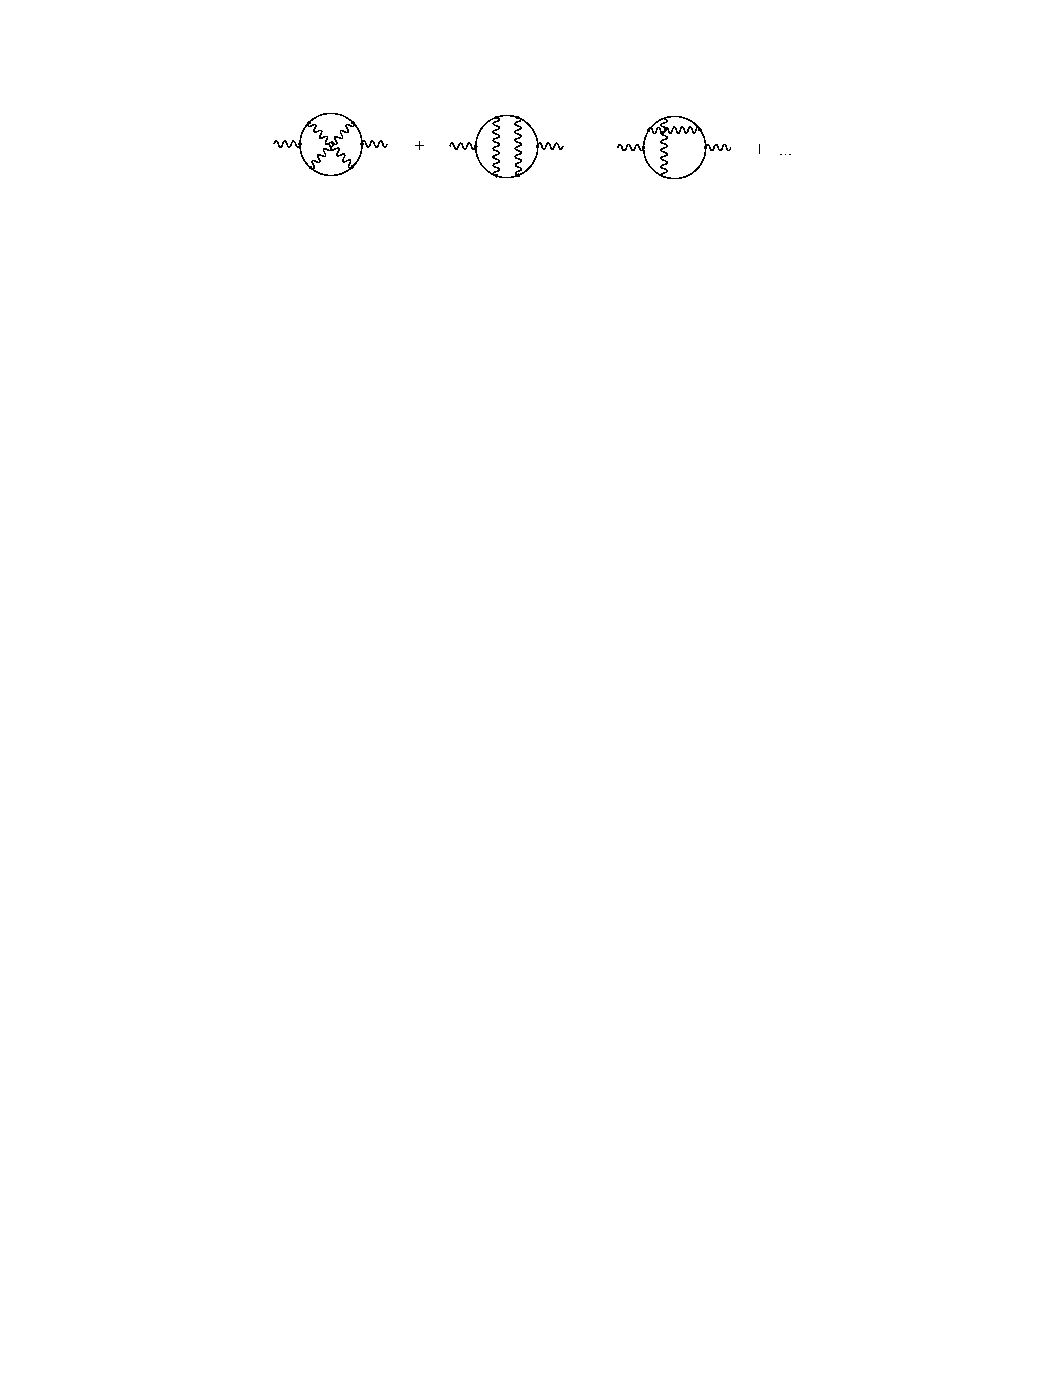
\includegraphics[width=1\textwidth]{BHSTW143loopphotonprop}
 \caption{
 Quenched diagrams contributing to the three loop QED photon propagator.
 From \refref{BHSTW14}.
 }
 \label{BHSTW143loopphotonprop}
\end{figure}
%%%%%%%%%%%%%%%%%%%%%%%%%%%%%%%%%%%%%%%%%%%%%%%%%

Thus, for the quenched scalar QED, the worldline integrals are expressed
in terms of $N$-photon propagators, the central ingredient that defines
the quenched gauge sets \refeq{quenchAnom}.
Unlike the Feynman parameter integrals for individual vertex graphs, they are
independent of the ordering of the momenta $k_1,\ldots,k_N$; the formula
\refeq{AhBaSc16(1)i} contains all $\approx N!$ ways of attaching the $N$
photons to the charged particle propagator.
The formulation combines combinatorially many Feynman diagrams into a single integral.
An example are the quenched contributions to the
three-loop photon propagator shown in \reffig{BHSTW143loopphotonprop}.

In QED the $N$-photon propagator formulation combines into one integral
all Feynman graphs related by permutations of photon legs along fermion
lines, that is, it should yield \emph{one} integral for a gauge set
$km'm$ defined in \refeq{quenchAnom}.
%, provided one may distinguish the leg-photons from the cross-photons.

\subsection{High-orders QED in worldline formalism}
\label{sect:highQEDworldline}

A non-perturbative formula for QED in a constant field, given for scalar
QED in 1982 by Affleck, Alvarez, and Manton\rf{AffAlMa82} is an example how the
worldline formalism can yield high-order information on QED amplitudes.
Huet, McKeon, and Schubert\rf{HuMcSc10} continue this in their 2010
%{\em {Euler-Heisenberg} lagrangians and asymptotic analysis in 1+1 {QED.
% Part I: Two}-loop}
%(no GaTech online access, \arXiv{1010.5315}):``
study of the l-electron loop, $N$-photon amplitudes in the limit of large
photon numbers and low photon energies, this time for 1+1 dimensional
scalar QED, in order to illustrate the large cancellations inside gauge
invariant classes of graphs.

Affleck \etal\rf{AffAlMa82} use the Feynman\rf{Feynman50} `worldline
path integral' representation of the quenched effective action for scalar
QED in the constant electric field, and calculate the amplitude in a
stationary path approximation. The stationary trajectory so obtained is a
circle with a field dependent radius, called ``instanton''  in this
context. The worldline action on this trajectory yields the correct
exponent, and the second variation determinant yields the correct  prefactor.
Using Borel analysis, they obtain non-perturbative information on the
on-shell renormalized $N$-photon amplitudes at large $N$ and low energies.

Parenthetically, independently and not by worldline formalism, but by
dint of difficult calculations and much deep physics intuition, Lebedev
and Ritus\rf{LebRit84} have arrived at a nonperturbative mass shift
interpretation for the spinor QED pair creation in constant electric
field in 1984.

For the quenched spinor QED (fermion lines decorated by photon exchanges)
closed-form expressions for general $N$ require the worldline
super-\,formalism\rf{Schubert01}, at the cost of introducing Fradkin
1966\rf{Fradkin66} Grassmann path integral,
or, alternatively,
the second order
formalism of Strassler\rf{Strassler92}.


% \item[2017-07-05 Christian] read
The  2017 G. Torgrimsson, Schneider,  Oertel and Schützhold\rf{TSOS17},
% {\em Dynamically assisted {Sauter-Schwinger} effect - non-perturbative
% versus perturbative aspects},
\arXiv{1703.09203}, sect.~3,
uses the $N$-photon formalism to determine a saddle and the asymptotic
form of two types of dynamically assisted {Sauter-Schwinger} effect.

The 2006 Dunne and Schubert\rf{DunSch06} study of scalar and spinor QED
$N$-photon amplitudes, in the quenched approximation (\ie, taking only
the diagrams with one electron loop) led to ``the following
generalization of Cvitanovi\'c's conjecture: the perturbation series
converges for all on-shell renormalized QED amplitudes at leading order
in $N_f$. It must be emphasized that the on-shell renormalization is
essential in all of the above.''
Unlike Cvitanovi\'c\rf{Cvit77b} purely numerical conjecture, theirs is a
sophisticated argument, buttressed by Borel dispersion relations.


\subsection{Electron magnetic moment in worldline formalism}
\label{sect:magMomWorldline}

Here we specialize the electron magnetic moment discussion of
\refsect{sect:magMom} to the quenched subsector.
$Z_1$,
$Z_2$, and % = (1-B)^{-1}$, and
$Z_3$,
are the respectively the vertex,
the electron wave function, and
the photon wave function
renormalization constants.
For quenched QED there are no
fermion loops, there are no vacuum polarization contribution to the charge
renormalization \refeq{IRstruct(3)}, $Z=Z_3=1$, so the bare coupling equals
the physical coupling, $\alpha_0= \alpha$.
Furthermore, $Z_1=Z_2$ by the Ward identity\rf{Ward50}.


%%%%%%%%%%%%%%% start inseert %%%%%%%%%%%%%%%%%%%%%%%%%%%%
%\section{Electron magnetic moment}
The anomalous magnetic moment of an electron $a = (g-2)/2$ is
given by the static limit of the magnetic form factor
$a=\tilde{F}_2(0)=M/(1+L)$ from \refeq{PRD10-74-III(2.2)},
with perturbative expansion
\beq
a = \frac{M(\alpha)}{1+L(\alpha)}
  =  \sum_{n=1}^\infty
          a^{(2n)}\left(\frac{\alpha}{\pi}\right)^{n}
\,,
\ee{IRstruct(1)Q}
where $Z_1=1+L =F_1(0)$, $M=F_2(0)$ are computed from the unrenormalized
on-shell values of proper vertex \refeq{BAGTB17(35-1)}, given by the sum
of all one-particle irreducible (1pI) electron-electron-photon vertex
diagrams with internal photon corrections (no electron loops).
Expanding $M$ and $L$ we have
\bea
a_{0}^{(2)} &=& M^{(2)}
            \continue
a_{0}^{(4)} &=& M^{(4)} - L^{(2)}M^{(2)}
            \label{PRD10-74-III(2.6)Q}\\
a_{0}^{(6)} &=& M^{(6)} - L^{(2)}M^{(4)} - (L^{(4)} - (L^{(2)})^2) M^{(2)}
\nnu
\eea
Each order in
\refeq{IRstruct(1)Q} is IR and UV finite, with the UV subdivergences are
cancelled by $L^{(2m)}$ counterterms in \refeq{PRD10-74-III(2.6)Q}.

A gauge set $km'm$ in expansion \refeq{quenchAnom} consists of all 1-particle irreducible vertex
diagrams without electron loops, with $k$ photons crossing the external
vertex (cross-photons) and $m [m']$ photons originating and terminating
on the incoming [outgoing] electron leg (leg-photons). One can assume
three different coupling, setting them all equal to $\alpha$ at the
end of the calculation,
\beq
a =
          \sum_{m'=0}^\infty\left(\frac{\alpha'}{\pi}\right)^{m'}
          \sum_{k=1}^\infty\left(\frac{\alpha_v}{\pi}\right)^{k}
          \sum_{m=0}^\infty\left(\frac{\alpha}{\pi}\right)^{m}
          a_{km'm}
\,.
\ee{quenchAnomQ}
The gauge set contributions are then
\bea
a^{(2)} &=& a_{100}
            \continue
a^{(4)} &=& a_{200} + a_{110} + a_{101}
            \label{gaugeSets}\\
a^{(6)} &=&  a_{300} + a_{210} + a_{201} +  a_{120} + a_{102} + a_{111}
            \continue
a^{(8)} &=& a_{400} + a_{310} + a_{301}  +  a_{220} + a_{202} + a_{211}
         +  a_{130} + a_{103} + a_{121} + a_{112}
            \continue
a^{(10)}&=& a_{500} + a_{410} + a_{401} +  a_{320} + a_{302} + a_{311}
         +  a_{230} + a_{203} + a_{221} + a_{212}
            \ceq
         +  a_{140} + a_{104} + a_{131} + a_{113} + a_{122}
\nnu
\eea




Both $L^{(2m)}$ and $M^{(2m)}$ can be evaluated in terms of
$N$-photon propagators.

\begin{enumerate}
  \item
To proceed, one needs something like a Bern-Kosower\rf{BerKos91} type
master formula for the electron line dressed with any number of photons,
with a single constant external (arbitrarily weak) magnetic field insertion.
% Schubert \etal\ have it (unpublished).
For the magnetic moment calculation, the external vertex is distinguished
by its
\(
\sigma^{\mu\nu}={1\over 2}[\gamma^{\mu},\gamma^{\nu}]
\)
form \refeq{BAGTB17(35-1)}, while all internal, virtual photon vertices
are of the usual $\gamma^{\mu}$ form.
  \item
Please write down
the worldline formula for the anomalous magnetic moment
of the electron $a=\tilde{F}_2(0)$, corresponding to Dirac trace
expression \refeq{PRD10-74-III(2.2)} for $M$.
  \item
As the external vertex transfers a (vanishing) momentum, the
incoming and outgoing electron on-mass shell legs are distinct, and thus
there are three kinds of $N$-photon propagators; $k$ photons crossing the
external vertex (cross-photons) and $m [m']$ photons originating and
terminating on the incoming [outgoing] electron leg (leg-photons). One
needs to prove in the worldline formalism that each $km'm$
integral (corresponding to a set of quenched set of 1-particle
irreducible Feynman vertex diagrams without electron loops) is separately
(i) a gauge set, and
(ii) the minimal gauge invariant set.
  \item
Hopefully the distinction motivates the  gauge set sign rule
\refeq{Cvit77b(5)}. Keep in mind, however, that this empirical rule is
already violated by the gauge set $(2,2,0)$.
  \item
Please write down
the worldline integral for one-loop anomaly $a_{0}^{(2)}$ in
\refeq{PRD10-74-III(2.6)}.
The first thing to verify is that the worldline $(1,0,0)$ integral
reproduces Schwinger's $\frac{1}{2}\left(\frac{\alpha}{\pi}\right)$
result\rf{Schwinger48}, exactly. That is an exercise in converting the
integral into Feynman-parametric form, already done several times for
other amplitudes.
  \item
Please write down the worldline integral for 2-loop anomaly
$a_{0}^{(4)}=M^{(4)}-L^{(2)}M^{(2)}$ in \refeq{PRD10-74-III(2.6)}.
Can $L^{(2)}M^{(2)}$ be absorbed into the integrand? If cancelations can
be made pointwise, that would obviate a need for constructing UV  (and
IR?) counterterms.
  \item
For 2-loop anomaly there are only 2 quenched gauge sets $km'm$:
$(2,0,0)$ and $(1,1,0)$, which equals $(1,0,1)$ by time reversal, see
\reffig{Cvit77bFig1} and \reftab{tabGaugeSets}.
So, reformulate the 2-loop calculation as two worldline integrals,
one for each gauge set.
Most likely, want to do the gauge set $(2,0,0)$ first, as it seems to
have simpler subdiagram structure (though not sure about that).
Do not attempt (for now) to evaluate these analytically (though
Broadhurst, Laporta,
Kreimer, \etc, would be interested to see whether some simplification
occurs), main thing is to understand that the UV renormalization works,
and that there are no intermediate IR divergences in this reformulation.
\end{enumerate}


\section{Volkov method}
\label{sect:Volkov}

In \refref{Volkov16} Volkov explains that $A_1^{(2n)}$ is free from
infrared divergences since they are removed by the on-shell
renormalization.
However, Volkov also states that there is no universal method in QED for
canceling IR divergences in the Feynman graphs analogous to the R
operation, and that the standard subtractive on-shell renormalization
cannot remove IR divergences point-by-point in Feynman-parametric space,
as it does for UV divergences. Moreover, it can generate additional
IR-divergences.

That QED on-mass shell amplitudes are IR-free must be an old result; even
I have several papers generalizing that to
QCD\rf{MassShell,IRstruct,QCDmshell,NPB81}. Tom Kinoshita and I solved
the problem of point-by-point removal of IR divergences in
Feynman-parametric space in my thesis\rf{CviKin74b}, with a
super-elegant formula (who needs forests?) for the UV and IR finite part
of amplitude $M_G$,
\beq
\Delta M_G =\prod_{ij}(1-I_{G/S_i})(1-K_{G/S_j}) M_G
\,,
\ee{UV-IRfiniteGcorr}
where the products are over all self-energy and vertex subdiagrams $S_i$
and $S_j$.
I have a bright memory of figuring out how to do it one quiet evening in
Ithaca, babysitting for a friend's toddler. But, as Volkov\rf{Volkov16}
and Aoyama \etal\rf{AoHaKiNiWa08} explain, our approach was apparently
not general enough to deal with the 4- and 5-loop contributions.

Volkov's algorithm is developed in {\em New method of computing the
contributions of graphs without lepton loops to the electron anomalous
magnetic moment in {QED}}\rf{Volkov17}. It is based on the ideas used for
proving UV-finiteness of renormalized Feynman
amplitudes\rf{Speer68,AnZaPo73}. He focuses on $n$-loop graphs with no
lepton loops, or, in the notation of these notes, $a^{(2n)}[V]$.
%
Volkov calculation groups Feynman graphs by self-energy graphs families
because they have similar integrand structure. In contrast to
\refrefs{CviKin74c,CarYao74,Carroll75,AoHaKiNi15} he does not evaluate
these self-energy graphs directly; all his calculations are performed
with vertex graphs, \ie, precisely what is needed to evaluate gauge sets
of \refsect{sect:finitness}. However, as illustrated in
\reffig{Cvit77bFig3}, each gauge-set vertex diagram belongs to a
different self-energy diagram, so Volkov calculation will require a major
reorganization of how integrands are generated, requiring months
of recoding.

So far Volkov  has evaluated the ladder graph
%(Figure \ref{fig_ladder})
and the fully crossed graph
%(Figure \ref{fig_crosses})
up to 5 loops. The cross graphs are of interest because they do not
contain divergent subgraphs, so their contributions only depend on the
gauge, but not on the choice of subtraction procedure.

While the contributions of individual vertex graphs (and self-energy
sets\rf{AoHaKiNi15}) are all over the place, all gauge sets are
insanely small up to order 8, and it would be very sweet to see that this
continues through order 10 (at least for the 5-loop graphs with no
electron loops).
My hunch is that starting with the gauge set $(5,0,0)$ of
\reftab{tabGaugeSets} ($5!$ vertex graphs, some of them symmetric pairs)
would be the most rewarding.
Stefano Laporta thinks it too hard, and suggests starting with the 5-loop
relative
$(1,3,1)$ (or $(1,2,2)$) of the 4-loop set $(1,2,1)$,
which would entail less than $5!$ vertex graphs (I have not counted
how many). As no high accuracy is needed, a numerical check of the QED
finiteness conjecture would good enough if the gauge sets evaluated
to two significant digits or so, but even that will need a lot of
computer time.

\section{Hopf algebraic approach}
\label{sect:HopfAlgebra}

Hopf algebraic approach of Kreimer and collaborators\rf{BrDeKr96,
Kreimer00, KreYea08, KisKre16} is very appealing - it is just that I
personally have no clue how to turn it into a direct $(g-2)$ gauge set
calculation. In the 2008 paper\rf{KreYea08}
\HREF{https://www2.mathematik.hu-berlin.de/~kreimer/} {Dirk Kreimer} and
\HREF{https://arxiv.org/find/math-ph,math/1/au:+Yeats_K/0/1/0/all/0/1}
{Karen Yeats} write:
    \begin{quote}
``One case where there is a natural interpretation is QED with a linear
number of generators, namely
\beq
X_1 = 1 + \sum_{k \geq 1}p(k)x^k
      \frac{X_1^{2k+1}}
           {(1-X_2)^{2k}(1-X_3)^{2k}}
\,,
\ee{KreYea08p413}
with $X_2$ and $X_3$ as before and with $p(k)$ linear, which corresponds
to counting with Cvitanovi\'c's gauge invariant sectors\rf{Cvit77b}.''
    \end{quote}
%{\bf 2017-05-31 Predrag}
Even in this simple case I do not see how this counts the gauge sets. My
generating function for $G_{2n}$, the number of gauge sets
(eq.~(7) in \refref{Cvit77b})  is
\beq
\sum_{n=1}^\infty G_{2n}
    =
      \frac{X}
           {(1+X)(1-X)^{3}}
\,.
\ee{Cvit77b(7)}

Broadhurst, Delbourgo and Kreimer\rf{BrDeKr96} 1996 {\em Unknotting the
polarized vacuum of quenched {QED}} unearthes much knot-theory magic,
leading to cancelations of ``transcedentals.'' While their
particular conjecture did not work out
in higher orders, the conceptual scheme might be another
route to proving the QED is finite - if there is some finite knot-theory
basis for expressing the value of every gauge set, and the gauge
invariance induced cancelations are so strong to lead to the large
cancelations of transcendentals (hyperlogarithms), then perhaps that
gives bounds on the size of each gauge set which are slower than
combinatorial. The number of different kinds of knots with $n$ crossings
is known to grow only exponentially, not faster.

Henry Ki{\ss}ler (on \refpage{sect:Hepp}) has a fresh idea for how to
approach the finiteness conjecture, using the \emph{Hepp bound},
see Panzer {\bf 2018-06-07} below.

Note that the Ki{\ss}ler and Kreimer\rf{KisKre16} definition of a ``gauge
set'' differs from \refeq{quenchAnom} used here. They organize a
gauge-dependent calculation into ``gauge sets'' of different parameter
dependence.

My notes on these papers are below, starting on \refpage{sect:BrDeKr96}.

%%%%%%%%%%%%%%%%%%%%%%%%%%%%%%%%%%%%%%%%%%%%%%%%%%%%%%%%%%%%%%%%%%%%%%%%%
% \section{Method of smooth conjugacies}
% \label{sect:scfpo}
    % reducesymm/QFT/scfpo.tex , called by finiteQED.tex
% Predrag                               jul 10 2017

\section{Method of smooth conjugacies}
\label{sect:scfpo}

\begin{quote}
\emph{If Feynman knew Poincar\'e: How to replace many diagrams by one}

In quantum field theory the standard Feynman diagram methods become
quickly unwieldy at higher orders. However,
% as students of these notes will not be shocked to hear,
it is frequently observed that the sums of Feynman diagrams, each
individually complicated, simplify miraculously to rather compact
expressions.

Here comes a possible reason why that can be traced back to Poincar\'e,
and is perhaps not something that a field theorist would instinctively
hark to as a method of computing perturbative corrections: make the
dynamics linear (``free'') by flattening out the vicinity of a path
integral extremum by a smooth nonlinear coordinate transformation.
%This does not come cheap, but
The resulting perturbative expansion is more compact than the standard
Feynman diagram perturbation theory.
\end{quote}

\noindent
The smooth conjugacy method sketched here would require some serious work
to make it a workable quantum field theory scheme. The reader might
prefer to skip straight to the worldline formalism
\refsect{sect:worldline}.

The periodic orbit theory is a classical, deterministic
theory\rf{ChaosBook} that describes nonlinear systems in ``chaotic'' (for
low-dimensional systems) or ``turbulent'' (for PDEs) regimes. The theory
allows us to calculate long time averages in a chaotic system as
expansions in terms of the periodic orbits (cycles) of the system. The
simplest example (the deterministic analogue of the quantum evolution
operator) is provided by the {\FPoper}
\beq
\Lop \rho(x')=\int\!\!dx\,\delta(f(x)-x')\rho(x)
\ee{FPoper}
for a {\em deterministic} map $f(x)$ which maps a density distribution
$\rho(x)$ forward one integer step in time. The periodic orbit theory relates the spectrum
of this operator and its weighted evolution operator generalizations to
the periodic orbits via trace formulas, \dzeta s and spec\-tral
det\-er\-min\-ants\rf{GasAlo93,ChaosBook}.

For quantum mechanics the periodic orbit theory is exact on the
semiclassical level\rf{gutbook}, whereas the quintessentially quantum
effects such as creeping, tunneling and diffraction have to be included
as corrections. In particular, the higher order $\hbar$ corrections can
be computed perturbatively by means of Feynman diagrammatic
expansions\rf{GasAlo93}.
We illustrate how this works by the parallel, but simpler example of {\em
stochastic} dynamics.
Cvitanovi\'{c}\rf{chfield} {\em {Chaotic Field Theory}: {A} sketch}
% ~predrag/articles/hongkong/hk.tex
is a programmatic statement how this theory might connect to quantum
field theory, and, by a way of motivation, an easy introduction into
different approaches to incorporating stochastic corrections into
classical dynamics.

What motivated the work\rf{noisy_Fred,conjug_Fred,diag_Fred}
summarized in \refref{chfield} is the fact that the form of perturbative
corrections for the stochastic problem  is the same as for the quantum
problem, and still the actual calculations are sufficiently simple that
one can explore more orders in perturbation theory than would be possible
for a full-fledged quantum theory.
For the simple system studied, the result is a stochastic analog of the
Gutzwiller trace formula with  the ``$\hbar$ corrections'' computed to
five orders beyond what has been attainable in the quantum-mechanical
applications. Already a discrete time,
1-dimensional discrete Langevin equation\rf{vKampen92,LM94},
\begin{equation}
x_{n+1}=f(x_n)+\sigma\xi_n
\,,\label{Langevin}
\end{equation}
with $\xi_n$ independent normalized random variables, suffices to reveal
the structure of perturbative corrections.
We treat a chaotic system with weak external noise by replacing the
deterministic evolution $\delta$-function kernel of {\FPoper}
\refeq{FPoper} by $\Lnoise{}$,  the Fokker-Planck kernel corresponding to
\refeq{Langevin}, a peaked noise distribution function
\beq
\Lnoise{}(x',x) =\delta_\sigma(f(x)-x')
\,.
\ee{Lnoise}
In the weak noise limit the kernel is sharply peaked, so it
makes sense to expand it
in terms of the Dirac delta function and
its derivatives:
\beq
	\delta_\sigma(y)
	=
	\sum_{m=0}^{\infty} {a_m \sigma^m \over m!} \, \delta^{(m)}(y)
	=
	\delta(y) +
	a_2 {\sigma^2 \over 2} \delta^{(2)}(y) +
	a_3 {\sigma^3 \over 6} \delta^{(3)}(y) + \dots
	\,.
\label{delSigExp}
\eeq
where
\[
	\delta^{(k)}(y) = {\pde^k \over \pde y^k} \delta(y)
	\,,
\]
and the coefficients $a_m$ depend on the choice of the kernel.
We have omitted the $\delta^{(1)}(y)$ term in the above because
in our applications we shall impose
the saddle-point condition, that is,
we shift $x$ by a constant to ensure that the noise peak corresponds
to $y=0$, so $\delta_\sigma^{'}(0)=0$.
For example, if $\delta_\sigma(y)$ is a Gaussian kernel,
it can be expanded as
\bea
	\delta_\sigma(y)
	&=&
	{1 \over \sqrt{2 \pi \sigma^2}} e^{-{y^2/2\sigma^2} }
	=
	\sum_{n=0}^{\infty}
	\frac{\sigma^{2n}}{n!2^n} \delta^{(2n)}(y)
	\continue
	&=&
	\delta(y) + {\sigma^2 \over 2} \delta^{(2)}(y)
	 + {\sigma^4 \over 8} \delta^{(4)}(y) + \cdots
	\,.
\label{delGaussExp}
\eea




% clipped from ~predrag/WWW/talks/UChicago99.html
% Trace formulas for stochastic evolution operators
% Feb. 10, 1999
Analogies between noise and quantum mechanics
can be explored by casting stochastic dynamics into path integral form (a
stoch\-astic Wiener integral). The periodic orbit theory is a
nonperturbative, ``WKB''  method for approximating such integrals, which
can then be improved by systematic perturbative corrections. In the weak
noise case the standard perturbation theory is an expansion in terms of
Feynman diagrams. For semiclassical quantum mechanics of a classically
chaotic system such calculation was first carried out by
Gaspard\rf{GasAlo93}. The stochastic version, implemented by Dettmann
\etal\rf{noisy_Fred}, reveals features not so readily apparent in the
quantum calculation. Perhaps some of these could be of interest to
Kreimer and collaborators, \refsect{sect:HopfAlgebra}.

The Feynman
diagram method becomes quickly unwieldy at higher orders.%
$\footnotemark\footnotetext{
The matrix method, introduced by Vattay \etal\rf{diag_Fred},
based on Rugh's\rf{hhrugh92} explicit matrix
representation of the {\evOper} will not be
discussed here. If one is interested in evaluating
numerically many orders of perturbation theory and many eigenvalues, this
method is unsurpassed.
}$
% ~predrag/articles/noise/conjug/conjug.tex clipping
%	Carl &  Predrag				27 oct 1998
However, in the Feynman diagram approach pursued in \refref{noisy_Fred},
the authors observe that the sums of Feynman diagrams simplify
miraculously to rather compact expressions.

Now the surprise; one can compute the same corrections faster and to a
higher order in perturbation theory by integrating over the neighborhood
of a given saddlepoint \emph{exactly} by means of a nonlinear change of
field variables. This elegant idea of flattening the neighborhood of a
saddlepoint, introduced by Mainieri \etal\rf{conjug_Fred}, and referred
to here as the {\em smooth conjugation method}, is perhaps an altogether
new idea in field theory. The idea, that  can be traced back to
Poincar\'e\rf{poincare}, injects into field theory a method standard in
the construction of normal forms for bifurcations\rf{Katok95}: perform a
smooth nonlinear coordinate transformation
$x = h(y)$,
$ f(x) = h(g(h^{-1}(x)))$
that flattens out the vicinity of a fixed point and makes the map {\em
linear} in an open neighborhood,
$ f(x) \to g(y) = {\bf J} \cdot y$.
\vspace{2ex}
\\
\centerline{
 ${
	\raisebox{-4.0ex}[5.5ex][4.5ex]
		 {
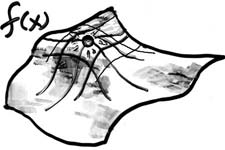
\includegraphics[height=10ex]{conjug-a}
		 }
        \atop
        \mbox{an arbitrary coordinatization}
        }$
~~~
$\Longrightarrow$
~~~
 ${
	\raisebox{-4.0ex}[5.5ex][4.5ex]
		 {
	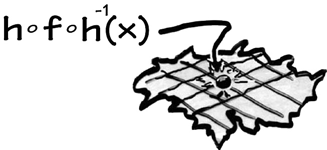
\includegraphics[height=10ex]{conjug-b}
		 }
        \atop
        \mbox{intrinsic, flat coordinates}
        }$
          }
\vspace{2ex}
\\
The resulting perturbative expansion turns out to be more compact than
the standard Feynman diagram perturbation theory; whether it is better
than the traditional loop expansions for computing field-theoretic
saddlepoint correction remains to be seen.

What is new is that the problem is being solved locally, periodic orbit
by periodic orbit, by translation to coordinates intrinsic to the
periodic orbit.

This local rectification of a map can be implemented only for isolated
non-degenerate fixed points (otherwise higher terms are required by the
normal form expansion around the point), and only in finite
neighborhoods, as the conjugating functions in general have finite radia
of convergence.

In this approach the neighborhood of each saddlepoint is rectified by an
appropriate nonlinear field transformation, with the focus shifted from
the dynamics in the original field variables to the properties of the
conjugacy transformation. The expressions thus obtained \emph{correspond
to sums} of Feynman diagrams, but are more compact.

We will try to explain this simplification in geometric terms that might
be applicable to more general field theoretic problems. The idea is this:
as the dynamics is nonlinear, why not search for a nonlinear field
transformation $\field = h(\tilde{\field})$ (a smooth conjugacy) that
makes the intrinsic coordinates as simple as possible? Schematically
--wrong in detail, but right in spirit-- find a smooth conjugacy such
that the action $S[\field] = S_0[\field] + S_I[\field]$ in the partition
function path integral becomes the free, quadratic action,
\beq
Z %[\source]
	 =  e^{W} %[\source]}
\,=\, \int [d\field] e^{S[\field]} % + \field \cdot \source}
\,=\, \int [d\tilde{\field}]
      \frac{1}{|\det \partial h(\tilde{\field})|^{1 \over 2}}
%      \, e^{\tilde{S}_0[\tilde{\field}]}
      \, e^{
      \frac{1}{2}
      \transp{\tilde{\field}}\frac{1}{\Delta}\tilde{\field}
            }
\,,
\label{Z-J}
\eeq
at the price of having the determinant of the
conjugacy Jacobian show up as a weight.

\refRef{noisy_Fred} treats the problem of computing the spectrum of this
operator by standard field-theoretic Feynman diagram expansions. Here we
formulate the perturbative expansion in terms of smooth conjugacies and
recursively evaluated derivatives. The procedure, which is relatively
easy to automatize, enables us to go one order further in the
perturbation theory, with much less computational effort than Feynman
diagrammatic expansions would require.

[TO BE CONTINUED]

%%%%%%%%%%%%%%%%%%%%%%%%%%%%%%%%%%%%%%%%%%%%%%%%%%%%%%%%%%%%%%%%%%%%%%%%%

\section{Summary}
\label{sect:Summary}

\begin{bartlett}{
\HREF{https://doi.org/10.1088/0954-3899/29/1/302}
{Everyone makes mistakes—including {Feynman}}
        }
\bauthor{
Toichiro Kinoshita\rf{Kinoshita03}
    }
\end{bartlett}
\bigskip

\noindent
Currently Sergey  A. Volkov is in the best position to check the QED
finiteness conjecture numerically, by computing the 5-loops gauge sets.

Worldline formalism could be useful on a qualitative level, as a way of
proving the finiteness of QED conjecture,
    \begin{enumerate}
  \item
Develop a saddle point expansion for the $N$-photon propagator
integrals, such that the
leading term explains the apparent $\approx \pm 1/2$ (or a multiple
thereof) size of each quenched gauge set. Affleck \etal\rf{AffAlMa82}
and G. Torgrimsson \etal\rf{TSOS17} show the way.
  \item
Use that to establish bounds on gauge sets for large orders, prove
finiteness of quenched QED. If that works, I trust electron loop
insertions will be next, and thereafter renormalons\rf{Lautrup77}, \etc,
will go \HREF{https://soundcloud.com/poets-org/notgogentle-mp3-5/s-2o7zI}
{gently into that good night}.
    \end{enumerate}
and in a precise way, as a new computational tool:
    \begin{enumerate}
  \item
Develop a worldline formulation of spinor QED in which each gauge set is
given by a computable integral, in a way to be fleshed out in
\refsect{sect:magMomWorldline}.
  \item
Parenthetically, a reformulation of the self-energy diagrams magnetic
moment calculation, \refsect{sect:selfEnergy}, would be an even greater
computational time saver - all quenched diagrams contributions calculated
at one go.
  \item
In either case, a
worldline formulation might make it possible to evaluate orders beyond
5-loops, as the number of gauge sets grows only polynomially. A win-win.
  \item
A gauge set is by definition UV and IR finite. The worldline formalism
quenched QED needs wave function
counterterms, as in \refeq{IRstruct(1)}.
  \item
Things get interesting with reformulating the quenched 3-loop calculation
as four worldline integrals / gauge sets, see \reffig{Cvit77bFig3} and
\reftab{tabGaugeSets}. In particular, the fermion line attachments of
different kinds of $N$-photon propagators now get intertwined.
  \item
One electron-loop insertion into $(1,0,0)$  might be the easiest
worldline integral to
evaluate, but I find the quenched sets a higher priority.
  \item
One photon-photon scattering electron-loop insertion into $(2,0,0)$ might
be the most tempting to evaluate, but I find the quenched sets a higher
priority.
    \end{enumerate}
My main problem at the moment (well, there are many:) is that nobody
seems to have written an explicit formula for the spinor QED anomalous
magnetic moment in the worldline formalism.

\newpage
% reducesymm/QFT/correspnd.tex
% $Author$ $Date$
% Predrag  switched to github.com               jul  8 2013

\section{Is QED finite? Correspondence}
\label{sect:correspnd}


\begin{bartlett}{
I am not sure I'll will tell you anything useful any time soon, as I'm a
lapsed field theorist, but here is for your amusement my
\HREF{https://vimeo.com/79605418} {recent rant}. To
cite my wife: ``You may well be right".
        }
\bauthor{
\HREF{http://www.goodreads.com/work/quotes/3226250-keep-the-aspidistra-flying}
{Keep the Aspidistra Flying!}
    }
\end{bartlett}
\bigskip



\begin{description}

\item[2007-03-18 Dirk Kreimer] % kreimer@ihes.fr via nbi.dk
I was pretty much looking forward to grab you for a chat on Dyson
Schwinger etc whilst in Bonn this starting week. Now I fail to be there
myself due to a stupid mechanical problem with a vertebrae.
Pondering about other options, let me just point out that the IHES
(www.ihes.fr) has an excellent visitor program. If you foresee some time
you fancy to pay us a visit, please go ahead.

I am running a little seminar at Boston whilst being there, so besides
what works out with IHES,  whenever you are available in the above
period, you are herewith invited for a talk at BU.
Would you be able to come for a seminar to Boston, Thu, Nov 29 this year?

\item[2011-08-23 Predrag] to Dirk:

I feel like some stuck-up god knows who for not having answered sooner -
but it is not that. I have been focusing on turbulence (with the goal of
using what I learn on Yang-Mills, eventually - if it works, Feynman
diagrammar will be of secondary importance, the first step is fully and
totally non-perturbative) so I feel like fraud talking about QFT when I
am suspended between the perturbative past and the elusive
non-perturbative future.

If someone wants to hear about turbulence as in
\HREF{http://ChaosBook.org/tutorials} {ChaosBook.org/tutorials}, I can do
that honestly - otherwise we wait until I actually do any QFT worth
hearing about...

I got \HREF{http://birdtracks.eu} {birdtracks.eu} published, finally -
you get 100 birdtracks per 1\$, a real deal if you are into that kind of
thing.

Guilty as Charged -
Predrag

\item[2011-08-26 Dirk]
June 01-05 2009 I am organizing a workshop at IHES. It has a
non-perturbative component via Dyson--Schwinger eqs. Would you be
interested to participate and come?

\item[2017-06-16 Dirk]
I will show your notes to
Henry Ki{\ss}ler\rf{Kissler16}   <kissler@physik.hu-berlin.de>
and
\HREF{http://people.physik.hu-berlin.de/~borinsky/}
{Michael Borinsky}\rf{Borinsky14,Borinsky17}    <borinsky@physik.hu-berlin.de> .

There should be a few people at Les Houches June 2018 who have something
to say about asymptotics of solutions of Dyson-Schwinger equation for
example.


\end{description}

%% Laporta17figuragau.tex %%%%%
%% compiled by  reducesymm/QFT/blog.tex
%%%%%%%%%%%%%%%%%%%%%%%%%%%%%%%%%%%%%%%%
\begin{figure}
\begin{center}
\begin{picture}(125,325)(70,50)
\thicklines
%%%
{
\put(+000.0,+200.0){\makebox(0,0)[lb]{
% fotone obliquo (0.000000,200.000000) (0.000000,205.000000)
   \qbezier(+000.0,+200.0)(+001.2,+201.2)(+000.0,+202.5)
   \qbezier(+000.0,+202.5)(-001.2,+203.8)(+000.0,+205.0)
% elettrone curvo (0.000000,200.000000) (-20.000000,160.000000) 1000.000000
% cerchio r=44721.365140 c=(-40010.000000,20180.000000) ang=(-26.536403,-26.593699)
   \qbezier(+000.0,+200.0)(-010.0,+180.0)(-020.0,+160.0)
% elettrone curvo (0.000000,200.000000) (20.000000,160.000000) 1000.000000
% cerchio r=44721.365140 c=(-39990.000000,-19820.000000) ang=(26.593699,26.536403)
   \qbezier(+000.0,+200.0)(+010.0,+180.0)(+020.0,+160.0)
% fotone obliquo (-14.142136,171.715729) (14.142136,171.715729)
   \qbezier(-014.1,+171.7)(-013.3,+170.8)(-012.4,+171.7)
   \qbezier(-012.4,+171.7)(-011.5,+172.6)(-010.6,+171.7)
   \qbezier(-010.6,+171.7)(-009.7,+170.8)(-008.8,+171.7)
   \qbezier(-008.8,+171.7)(-008.0,+172.6)(-007.1,+171.7)
   \qbezier(-007.1,+171.7)(-006.2,+170.8)(-005.3,+171.7)
   \qbezier(-005.3,+171.7)(-004.4,+172.6)(-003.5,+171.7)
   \qbezier(-003.5,+171.7)(-002.7,+170.8)(-001.8,+171.7)
   \qbezier(-001.8,+171.7)(-000.9,+172.6)(+000.0,+171.7)
   \qbezier(+000.0,+171.7)(+000.9,+170.8)(+001.8,+171.7)
   \qbezier(+001.8,+171.7)(+002.7,+172.6)(+003.5,+171.7)
   \qbezier(+003.5,+171.7)(+004.4,+170.8)(+005.3,+171.7)
   \qbezier(+005.3,+171.7)(+006.2,+172.6)(+007.1,+171.7)
   \qbezier(+007.1,+171.7)(+008.0,+170.8)(+008.8,+171.7)
   \qbezier(+008.8,+171.7)(+009.7,+172.6)(+010.6,+171.7)
   \qbezier(+010.6,+171.7)(+011.5,+170.8)(+012.4,+171.7)
   \qbezier(+012.4,+171.7)(+013.3,+172.6)(+014.1,+171.7)
% fotone curvo (5.303301,189.393398) (10.000000,180.000000) 0.100000
% fotone semicircolare r=5.355061 c=(6.712311,184.227029) ang=(105.255119,-52.125016)
% n=8
   \qbezier(+005.3,+189.4)(+006.3,+188.7)(+007.1,+189.6)
   \qbezier(+007.1,+189.6)(+008.3,+190.3)(+008.9,+189.1)
   \qbezier(+008.9,+189.1)(+009.2,+187.9)(+010.4,+188.1)
   \qbezier(+010.4,+188.1)(+011.7,+187.9)(+011.5,+186.6)
   \qbezier(+011.5,+186.6)(+011.0,+185.5)(+012.0,+184.9)
   \qbezier(+012.0,+184.9)(+013.0,+183.9)(+011.9,+183.0)
   \qbezier(+011.9,+183.0)(+010.8,+182.5)(+011.2,+181.4)
   \qbezier(+011.2,+181.4)(+011.3,+180.0)(+010.0,+180.0)
% fotone curvo (12.247449,175.505103) (17.320508,165.358984) 0.100000
% fotone semicircolare r=5.784178 c=(13.769367,169.924737) ang=(105.255119,-52.125016)
% n=9
   \qbezier(+012.2,+175.5)(+013.2,+174.8)(+014.0,+175.7)
   \qbezier(+014.0,+175.7)(+015.0,+176.5)(+015.7,+175.4)
   \qbezier(+015.7,+175.4)(+016.1,+174.2)(+017.3,+174.5)
   \qbezier(+017.3,+174.5)(+018.6,+174.6)(+018.5,+173.3)
   \qbezier(+018.5,+173.3)(+018.2,+172.1)(+019.3,+171.7)
   \qbezier(+019.3,+171.7)(+020.3,+171.0)(+019.6,+170.0)
   \qbezier(+019.6,+170.0)(+018.6,+169.2)(+019.3,+168.2)
   \qbezier(+019.3,+168.2)(+019.8,+167.0)(+018.5,+166.6)
   \qbezier(+018.5,+166.6)(+017.3,+166.5)(+017.3,+165.4)
% fotone curvo (15.811388,168.377223) (18.708287,162.583426) -0.100000
% fotone semicircolare r=3.302973 c=(17.839217,165.770015) ang=(127.874984,285.255119)
% n=5
   \qbezier(+015.8,+168.4)(+014.5,+168.2)(+014.7,+166.9)
   \qbezier(+014.7,+166.9)(+015.4,+166.0)(+014.6,+165.1)
   \qbezier(+014.6,+165.1)(+014.1,+163.9)(+015.4,+163.5)
   \qbezier(+015.4,+163.5)(+016.5,+163.7)(+016.9,+162.6)
   \qbezier(+016.9,+162.6)(+017.8,+161.6)(+018.7,+162.6)
\put(+000.0,+152.0){\makebox(0,0){$(1)$}}
}}
\put(+025.0,+200.0){\makebox(0,0)[lb]{
% fotone obliquo (25.000000,200.000000) (25.000000,205.000000)
   \qbezier(+025.0,+200.0)(+026.2,+201.2)(+025.0,+202.5)
   \qbezier(+025.0,+202.5)(+023.8,+203.8)(+025.0,+205.0)
% elettrone curvo (25.000000,200.000000) (5.000000,160.000000) 1000.000000
% cerchio r=44721.365140 c=(-39985.000000,20180.000000) ang=(-26.536403,-26.593699)
   \qbezier(+025.0,+200.0)(+015.0,+180.0)(+005.0,+160.0)
% elettrone curvo (25.000000,200.000000) (45.000000,160.000000) 1000.000000
% cerchio r=44721.365140 c=(-39965.000000,-19820.000000) ang=(26.593699,26.536403)
   \qbezier(+025.0,+200.0)(+035.0,+180.0)(+045.0,+160.0)
% fotone obliquo (14.309550,178.619101) (35.690450,178.619101)
   \qbezier(+014.3,+178.6)(+015.2,+177.7)(+016.1,+178.6)
   \qbezier(+016.1,+178.6)(+017.0,+179.5)(+017.9,+178.6)
   \qbezier(+017.9,+178.6)(+018.8,+177.7)(+019.7,+178.6)
   \qbezier(+019.7,+178.6)(+020.5,+179.5)(+021.4,+178.6)
   \qbezier(+021.4,+178.6)(+022.3,+177.7)(+023.2,+178.6)
   \qbezier(+023.2,+178.6)(+024.1,+179.5)(+025.0,+178.6)
   \qbezier(+025.0,+178.6)(+025.9,+177.7)(+026.8,+178.6)
   \qbezier(+026.8,+178.6)(+027.7,+179.5)(+028.6,+178.6)
   \qbezier(+028.6,+178.6)(+029.5,+177.7)(+030.3,+178.6)
   \qbezier(+030.3,+178.6)(+031.2,+179.5)(+032.1,+178.6)
   \qbezier(+032.1,+178.6)(+033.0,+177.7)(+033.9,+178.6)
   \qbezier(+033.9,+178.6)(+034.8,+179.5)(+035.7,+178.6)
% fotone obliquo (8.096915,166.193830) (41.903085,166.193830)
   \qbezier(+008.1,+166.2)(+009.0,+165.3)(+009.9,+166.2)
   \qbezier(+009.9,+166.2)(+010.8,+167.1)(+011.7,+166.2)
   \qbezier(+011.7,+166.2)(+012.5,+165.3)(+013.4,+166.2)
   \qbezier(+013.4,+166.2)(+014.3,+167.1)(+015.2,+166.2)
   \qbezier(+015.2,+166.2)(+016.1,+165.3)(+017.0,+166.2)
   \qbezier(+017.0,+166.2)(+017.9,+167.1)(+018.8,+166.2)
   \qbezier(+018.8,+166.2)(+019.7,+165.3)(+020.6,+166.2)
   \qbezier(+020.6,+166.2)(+021.4,+167.1)(+022.3,+166.2)
   \qbezier(+022.3,+166.2)(+023.2,+165.3)(+024.1,+166.2)
   \qbezier(+024.1,+166.2)(+025.0,+167.1)(+025.9,+166.2)
   \qbezier(+025.9,+166.2)(+026.8,+165.3)(+027.7,+166.2)
   \qbezier(+027.7,+166.2)(+028.6,+167.1)(+029.4,+166.2)
   \qbezier(+029.4,+166.2)(+030.3,+165.3)(+031.2,+166.2)
   \qbezier(+031.2,+166.2)(+032.1,+167.1)(+033.0,+166.2)
   \qbezier(+033.0,+166.2)(+033.9,+165.3)(+034.8,+166.2)
   \qbezier(+034.8,+166.2)(+035.7,+167.1)(+036.6,+166.2)
   \qbezier(+036.6,+166.2)(+037.5,+165.3)(+038.3,+166.2)
   \qbezier(+038.3,+166.2)(+039.2,+167.1)(+040.1,+166.2)
   \qbezier(+040.1,+166.2)(+041.0,+165.3)(+041.9,+166.2)
% fotone curvo (32.559289,184.881421) (38.093073,173.813853) 0.100000
% fotone semicircolare r=6.309484 c=(34.219425,178.794259) ang=(105.255119,-52.125016)
% n=9
   \qbezier(+032.6,+184.9)(+033.6,+184.1)(+034.5,+185.1)
   \qbezier(+034.5,+185.1)(+035.6,+185.9)(+036.3,+184.7)
   \qbezier(+036.3,+184.7)(+036.8,+183.5)(+038.0,+183.8)
   \qbezier(+038.0,+183.8)(+039.4,+183.8)(+039.4,+182.4)
   \qbezier(+039.4,+182.4)(+039.0,+181.2)(+040.2,+180.7)
   \qbezier(+040.2,+180.7)(+041.4,+179.9)(+040.5,+178.8)
   \qbezier(+040.5,+178.8)(+039.5,+178.0)(+040.2,+176.9)
   \qbezier(+040.2,+176.9)(+040.7,+175.6)(+039.4,+175.2)
   \qbezier(+039.4,+175.2)(+038.1,+175.1)(+038.1,+173.8)
% fotone curvo (40.118579,169.762842) (43.516402,162.967196) 0.100000
% fotone semicircolare r=3.874114 c=(41.137926,166.025237) ang=(105.255119,-52.125016)
% n=6
   \qbezier(+040.1,+169.8)(+041.0,+169.0)(+041.9,+169.8)
   \qbezier(+041.9,+169.8)(+043.1,+170.3)(+043.5,+169.1)
   \qbezier(+043.5,+169.1)(+043.5,+168.0)(+044.6,+167.8)
   \qbezier(+044.6,+167.8)(+045.7,+167.1)(+045.0,+166.0)
   \qbezier(+045.0,+166.0)(+044.1,+165.4)(+044.6,+164.3)
   \qbezier(+044.6,+164.3)(+044.8,+163.0)(+043.5,+163.0)
\put(+025.0,+152.0){\makebox(0,0){$(2)$}}
}}
\put(+050.0,+200.0){\makebox(0,0)[lb]{
% fotone obliquo (50.000000,200.000000) (50.000000,205.000000)
   \qbezier(+050.0,+200.0)(+051.2,+201.2)(+050.0,+202.5)
   \qbezier(+050.0,+202.5)(+048.8,+203.8)(+050.0,+205.0)
% elettrone curvo (50.000000,200.000000) (30.000000,160.000000) 1000.000000
% cerchio r=44721.365140 c=(-39960.000000,20180.000000) ang=(-26.536403,-26.593699)
   \qbezier(+050.0,+200.0)(+040.0,+180.0)(+030.0,+160.0)
% elettrone curvo (50.000000,200.000000) (70.000000,160.000000) 1000.000000
% cerchio r=44721.365140 c=(-39940.000000,-19820.000000) ang=(26.593699,26.536403)
   \qbezier(+050.0,+200.0)(+060.0,+180.0)(+070.0,+160.0)
% fotone obliquo (33.670068,167.340137) (66.329932,167.340137)
   \qbezier(+033.7,+167.3)(+034.5,+166.5)(+035.4,+167.3)
   \qbezier(+035.4,+167.3)(+036.2,+168.2)(+037.1,+167.3)
   \qbezier(+037.1,+167.3)(+038.0,+166.5)(+038.8,+167.3)
   \qbezier(+038.8,+167.3)(+039.7,+168.2)(+040.5,+167.3)
   \qbezier(+040.5,+167.3)(+041.4,+166.5)(+042.3,+167.3)
   \qbezier(+042.3,+167.3)(+043.1,+168.2)(+044.0,+167.3)
   \qbezier(+044.0,+167.3)(+044.8,+166.5)(+045.7,+167.3)
   \qbezier(+045.7,+167.3)(+046.6,+168.2)(+047.4,+167.3)
   \qbezier(+047.4,+167.3)(+048.3,+166.5)(+049.1,+167.3)
   \qbezier(+049.1,+167.3)(+050.0,+168.2)(+050.9,+167.3)
   \qbezier(+050.9,+167.3)(+051.7,+166.5)(+052.6,+167.3)
   \qbezier(+052.6,+167.3)(+053.4,+168.2)(+054.3,+167.3)
   \qbezier(+054.3,+167.3)(+055.2,+166.5)(+056.0,+167.3)
   \qbezier(+056.0,+167.3)(+056.9,+168.2)(+057.7,+167.3)
   \qbezier(+057.7,+167.3)(+058.6,+166.5)(+059.5,+167.3)
   \qbezier(+059.5,+167.3)(+060.3,+168.2)(+061.2,+167.3)
   \qbezier(+061.2,+167.3)(+062.0,+166.5)(+062.9,+167.3)
   \qbezier(+062.9,+167.3)(+063.8,+168.2)(+064.6,+167.3)
   \qbezier(+064.6,+167.3)(+065.5,+166.5)(+066.3,+167.3)
% fotone curvo (35.857864,171.715729) (31.742581,163.485163) -0.100000
% fotone semicircolare r=4.692144 c=(34.623279,167.188917) ang=(74.744881,232.125016)
% n=7
   \qbezier(+035.9,+171.7)(+035.0,+172.8)(+034.0,+171.8)
   \qbezier(+034.0,+171.8)(+033.4,+170.8)(+032.3,+171.3)
   \qbezier(+032.3,+171.3)(+031.0,+171.4)(+030.9,+170.1)
   \qbezier(+030.9,+170.1)(+031.2,+168.9)(+030.1,+168.4)
   \qbezier(+030.1,+168.4)(+029.0,+167.6)(+030.0,+166.6)
   \qbezier(+030.0,+166.6)(+031.0,+166.0)(+030.5,+164.9)
   \qbezier(+030.5,+164.9)(+030.4,+163.5)(+031.7,+163.5)
% fotone curvo (64.142136,171.715729) (68.257419,163.485163) 0.100000
% fotone semicircolare r=4.692144 c=(65.376721,167.188917) ang=(105.255119,-52.125016)
% n=7
   \qbezier(+064.1,+171.7)(+065.1,+171.0)(+066.0,+171.8)
   \qbezier(+066.0,+171.8)(+067.1,+172.5)(+067.7,+171.3)
   \qbezier(+067.7,+171.3)(+067.9,+170.1)(+069.1,+170.1)
   \qbezier(+069.1,+170.1)(+070.4,+169.7)(+069.9,+168.4)
   \qbezier(+069.9,+168.4)(+069.2,+167.5)(+070.0,+166.6)
   \qbezier(+070.0,+166.6)(+070.7,+165.4)(+069.5,+164.9)
   \qbezier(+069.5,+164.9)(+068.2,+164.7)(+068.3,+163.5)
% fotone curvo (56.123724,187.752551) (61.547005,176.905989) 0.100000
% fotone semicircolare r=6.183492 c=(57.750709,181.786942) ang=(105.255119,-52.125016)
% n=9
   \qbezier(+056.1,+187.8)(+057.2,+187.0)(+058.0,+188.0)
   \qbezier(+058.0,+188.0)(+059.1,+188.8)(+059.8,+187.6)
   \qbezier(+059.8,+187.6)(+060.3,+186.4)(+061.5,+186.7)
   \qbezier(+061.5,+186.7)(+062.9,+186.7)(+062.8,+185.4)
   \qbezier(+062.8,+185.4)(+062.5,+184.1)(+063.6,+183.7)
   \qbezier(+063.6,+183.7)(+064.8,+182.9)(+063.9,+181.8)
   \qbezier(+063.9,+181.8)(+062.9,+181.0)(+063.7,+180.0)
   \qbezier(+063.7,+180.0)(+064.1,+178.7)(+062.8,+178.3)
   \qbezier(+062.8,+178.3)(+061.6,+178.2)(+061.5,+176.9)
\put(+050.0,+152.0){\makebox(0,0){$(3)$}}
}}
\put(+075.0,+200.0){\makebox(0,0)[lb]{
% fotone obliquo (75.000000,200.000000) (75.000000,205.000000)
   \qbezier(+075.0,+200.0)(+076.2,+201.2)(+075.0,+202.5)
   \qbezier(+075.0,+202.5)(+073.8,+203.8)(+075.0,+205.0)
% elettrone curvo (75.000000,200.000000) (55.000000,160.000000) 1000.000000
% cerchio r=44721.365140 c=(-39935.000000,20180.000000) ang=(-26.536403,-26.593699)
   \qbezier(+075.0,+200.0)(+065.0,+180.0)(+055.0,+160.0)
% elettrone curvo (75.000000,200.000000) (95.000000,160.000000) 1000.000000
% cerchio r=44721.365140 c=(-39915.000000,-19820.000000) ang=(26.593699,26.536403)
   \qbezier(+075.0,+200.0)(+085.0,+180.0)(+095.0,+160.0)
% fotone obliquo (66.835034,183.670068) (91.329932,167.340137)
   \qbezier(+066.8,+183.7)(+067.1,+182.5)(+068.3,+182.7)
   \qbezier(+068.3,+182.7)(+069.5,+182.9)(+069.7,+181.7)
   \qbezier(+069.7,+181.7)(+070.0,+180.5)(+071.2,+180.8)
   \qbezier(+071.2,+180.8)(+072.4,+181.0)(+072.6,+179.8)
   \qbezier(+072.6,+179.8)(+072.8,+178.6)(+074.0,+178.9)
   \qbezier(+074.0,+178.9)(+075.2,+179.1)(+075.5,+177.9)
   \qbezier(+075.5,+177.9)(+075.7,+176.7)(+076.9,+176.9)
   \qbezier(+076.9,+176.9)(+078.1,+177.2)(+078.4,+176.0)
   \qbezier(+078.4,+176.0)(+078.6,+174.8)(+079.8,+175.0)
   \qbezier(+079.8,+175.0)(+081.0,+175.3)(+081.2,+174.1)
   \qbezier(+081.2,+174.1)(+081.5,+172.9)(+082.7,+173.1)
   \qbezier(+082.7,+173.1)(+083.9,+173.3)(+084.1,+172.1)
   \qbezier(+084.1,+172.1)(+084.4,+170.9)(+085.6,+171.2)
   \qbezier(+085.6,+171.2)(+086.8,+171.4)(+087.0,+170.2)
   \qbezier(+087.0,+170.2)(+087.2,+169.0)(+088.4,+169.3)
   \qbezier(+088.4,+169.3)(+089.6,+169.5)(+089.9,+168.3)
   \qbezier(+089.9,+168.3)(+090.1,+167.1)(+091.3,+167.3)
% fotone obliquo (58.670068,167.340137) (83.164966,183.670068)
   \qbezier(+058.7,+167.3)(+059.9,+167.1)(+060.1,+168.3)
   \qbezier(+060.1,+168.3)(+060.4,+169.5)(+061.6,+169.3)
   \qbezier(+061.6,+169.3)(+062.8,+169.0)(+063.0,+170.2)
   \qbezier(+063.0,+170.2)(+063.2,+171.4)(+064.4,+171.2)
   \qbezier(+064.4,+171.2)(+065.6,+170.9)(+065.9,+172.1)
   \qbezier(+065.9,+172.1)(+066.1,+173.3)(+067.3,+173.1)
   \qbezier(+067.3,+173.1)(+068.5,+172.9)(+068.8,+174.1)
   \qbezier(+068.8,+174.1)(+069.0,+175.3)(+070.2,+175.0)
   \qbezier(+070.2,+175.0)(+071.4,+174.8)(+071.6,+176.0)
   \qbezier(+071.6,+176.0)(+071.9,+177.2)(+073.1,+176.9)
   \qbezier(+073.1,+176.9)(+074.3,+176.7)(+074.5,+177.9)
   \qbezier(+074.5,+177.9)(+074.8,+179.1)(+076.0,+178.9)
   \qbezier(+076.0,+178.9)(+077.2,+178.6)(+077.4,+179.8)
   \qbezier(+077.4,+179.8)(+077.6,+181.0)(+078.8,+180.8)
   \qbezier(+078.8,+180.8)(+080.0,+180.5)(+080.3,+181.7)
   \qbezier(+080.3,+181.7)(+080.5,+182.9)(+081.7,+182.7)
   \qbezier(+081.7,+182.7)(+082.9,+182.5)(+083.2,+183.7)
% fotone curvo (60.857864,171.715729) (56.742581,163.485163) -0.100000
% fotone semicircolare r=4.692144 c=(59.623279,167.188917) ang=(74.744881,232.125016)
% n=7
   \qbezier(+060.9,+171.7)(+060.0,+172.8)(+059.0,+171.8)
   \qbezier(+059.0,+171.8)(+058.4,+170.8)(+057.3,+171.3)
   \qbezier(+057.3,+171.3)(+056.0,+171.4)(+055.9,+170.1)
   \qbezier(+055.9,+170.1)(+056.2,+168.9)(+055.1,+168.4)
   \qbezier(+055.1,+168.4)(+054.0,+167.6)(+055.0,+166.6)
   \qbezier(+055.0,+166.6)(+056.0,+166.0)(+055.5,+164.9)
   \qbezier(+055.5,+164.9)(+055.4,+163.5)(+056.7,+163.5)
% fotone curvo (85.526385,178.947231) (89.142136,171.715729) 0.100000
% fotone semicircolare r=4.122590 c=(86.611110,174.969905) ang=(105.255119,-52.125016)
% n=6
   \qbezier(+085.5,+178.9)(+086.5,+178.2)(+087.4,+179.0)
   \qbezier(+087.4,+179.0)(+088.7,+179.6)(+089.1,+178.3)
   \qbezier(+089.1,+178.3)(+089.1,+177.0)(+090.3,+176.8)
   \qbezier(+090.3,+176.8)(+091.5,+176.1)(+090.7,+175.0)
   \qbezier(+090.7,+175.0)(+089.7,+174.3)(+090.3,+173.2)
   \qbezier(+090.3,+173.2)(+090.5,+171.8)(+089.1,+171.7)
\put(+075.0,+152.0){\makebox(0,0){$(4)$}}
}}
\put(+100.0,+200.0){\makebox(0,0)[lb]{
% fotone obliquo (100.000000,200.000000) (100.000000,205.000000)
   \qbezier(+100.0,+200.0)(+101.2,+201.2)(+100.0,+202.5)
   \qbezier(+100.0,+202.5)(+098.8,+203.8)(+100.0,+205.0)
% elettrone curvo (100.000000,200.000000) (80.000000,160.000000) 1000.000000
% cerchio r=44721.365140 c=(-39910.000000,20180.000000) ang=(-26.536403,-26.593699)
   \qbezier(+100.0,+200.0)(+090.0,+180.0)(+080.0,+160.0)
% elettrone curvo (100.000000,200.000000) (120.000000,160.000000) 1000.000000
% cerchio r=44721.365140 c=(-39890.000000,-19820.000000) ang=(26.593699,26.536403)
   \qbezier(+100.0,+200.0)(+110.0,+180.0)(+120.0,+160.0)
% fotone obliquo (91.835034,183.670068) (114.142136,171.715729)
   \qbezier(+091.8,+183.7)(+092.2,+182.4)(+093.4,+182.8)
   \qbezier(+093.4,+182.8)(+094.7,+183.2)(+095.0,+182.0)
   \qbezier(+095.0,+182.0)(+095.4,+180.7)(+096.6,+181.1)
   \qbezier(+096.6,+181.1)(+097.8,+181.5)(+098.2,+180.3)
   \qbezier(+098.2,+180.3)(+098.6,+179.0)(+099.8,+179.4)
   \qbezier(+099.8,+179.4)(+101.0,+179.8)(+101.4,+178.5)
   \qbezier(+101.4,+178.5)(+101.8,+177.3)(+103.0,+177.7)
   \qbezier(+103.0,+177.7)(+104.2,+178.1)(+104.6,+176.8)
   \qbezier(+104.6,+176.8)(+105.0,+175.6)(+106.2,+176.0)
   \qbezier(+106.2,+176.0)(+107.4,+176.4)(+107.8,+175.1)
   \qbezier(+107.8,+175.1)(+108.1,+173.9)(+109.4,+174.3)
   \qbezier(+109.4,+174.3)(+110.6,+174.6)(+111.0,+173.4)
   \qbezier(+111.0,+173.4)(+111.3,+172.2)(+112.5,+172.6)
   \qbezier(+112.5,+172.6)(+113.8,+172.9)(+114.1,+171.7)
% fotone obliquo (85.857864,171.715729) (108.164966,183.670068)
   \qbezier(+085.9,+171.7)(+087.1,+171.3)(+087.5,+172.6)
   \qbezier(+087.5,+172.6)(+087.8,+173.8)(+089.0,+173.4)
   \qbezier(+089.0,+173.4)(+090.3,+173.1)(+090.6,+174.3)
   \qbezier(+090.6,+174.3)(+091.0,+175.5)(+092.2,+175.1)
   \qbezier(+092.2,+175.1)(+093.5,+174.8)(+093.8,+176.0)
   \qbezier(+093.8,+176.0)(+094.2,+177.2)(+095.4,+176.8)
   \qbezier(+095.4,+176.8)(+096.6,+176.5)(+097.0,+177.7)
   \qbezier(+097.0,+177.7)(+097.4,+178.9)(+098.6,+178.5)
   \qbezier(+098.6,+178.5)(+099.8,+178.2)(+100.2,+179.4)
   \qbezier(+100.2,+179.4)(+100.6,+180.6)(+101.8,+180.3)
   \qbezier(+101.8,+180.3)(+103.0,+179.9)(+103.4,+181.1)
   \qbezier(+103.4,+181.1)(+103.8,+182.3)(+105.0,+182.0)
   \qbezier(+105.0,+182.0)(+106.2,+181.6)(+106.6,+182.8)
   \qbezier(+106.6,+182.8)(+106.9,+184.0)(+108.2,+183.7)
% fotone obliquo (81.742581,163.485163) (118.257419,163.485163)
   \qbezier(+081.7,+163.5)(+082.6,+162.6)(+083.5,+163.5)
   \qbezier(+083.5,+163.5)(+084.4,+164.4)(+085.2,+163.5)
   \qbezier(+085.2,+163.5)(+086.1,+162.6)(+087.0,+163.5)
   \qbezier(+087.0,+163.5)(+087.8,+164.4)(+088.7,+163.5)
   \qbezier(+088.7,+163.5)(+089.6,+162.6)(+090.4,+163.5)
   \qbezier(+090.4,+163.5)(+091.3,+164.4)(+092.2,+163.5)
   \qbezier(+092.2,+163.5)(+093.0,+162.6)(+093.9,+163.5)
   \qbezier(+093.9,+163.5)(+094.8,+164.4)(+095.7,+163.5)
   \qbezier(+095.7,+163.5)(+096.5,+162.6)(+097.4,+163.5)
   \qbezier(+097.4,+163.5)(+098.3,+164.4)(+099.1,+163.5)
   \qbezier(+099.1,+163.5)(+100.0,+162.6)(+100.9,+163.5)
   \qbezier(+100.9,+163.5)(+101.7,+164.4)(+102.6,+163.5)
   \qbezier(+102.6,+163.5)(+103.5,+162.6)(+104.3,+163.5)
   \qbezier(+104.3,+163.5)(+105.2,+164.4)(+106.1,+163.5)
   \qbezier(+106.1,+163.5)(+107.0,+162.6)(+107.8,+163.5)
   \qbezier(+107.8,+163.5)(+108.7,+164.4)(+109.6,+163.5)
   \qbezier(+109.6,+163.5)(+110.4,+162.6)(+111.3,+163.5)
   \qbezier(+111.3,+163.5)(+112.2,+164.4)(+113.0,+163.5)
   \qbezier(+113.0,+163.5)(+113.9,+162.6)(+114.8,+163.5)
   \qbezier(+114.8,+163.5)(+115.6,+164.4)(+116.5,+163.5)
   \qbezier(+116.5,+163.5)(+117.4,+162.6)(+118.3,+163.5)
% fotone curvo (111.547005,176.905989) (116.329932,167.340137) 0.100000
% fotone semicircolare r=5.453375 c=(112.981883,171.644770) ang=(105.255119,-52.125016)
% n=8
   \qbezier(+111.5,+176.9)(+112.6,+176.2)(+113.4,+177.1)
   \qbezier(+113.4,+177.1)(+114.6,+177.8)(+115.2,+176.6)
   \qbezier(+115.2,+176.6)(+115.5,+175.4)(+116.8,+175.6)
   \qbezier(+116.8,+175.6)(+118.1,+175.4)(+117.9,+174.1)
   \qbezier(+117.9,+174.1)(+117.3,+173.0)(+118.4,+172.3)
   \qbezier(+118.4,+172.3)(+119.3,+171.3)(+118.3,+170.4)
   \qbezier(+118.3,+170.4)(+117.2,+169.9)(+117.6,+168.7)
   \qbezier(+117.6,+168.7)(+117.7,+167.4)(+116.3,+167.3)
\put(+100.0,+152.0){\makebox(0,0){$(5)$}}
}}
\put(+000.0,+165.0){\makebox(0,0)[lb]{
% fotone obliquo (0.000000,165.000000) (0.000000,170.000000)
   \qbezier(+000.0,+165.0)(+001.2,+166.2)(+000.0,+167.5)
   \qbezier(+000.0,+167.5)(-001.2,+168.8)(+000.0,+170.0)
% elettrone curvo (0.000000,165.000000) (-20.000000,125.000000) 1000.000000
% cerchio r=44721.365140 c=(-40010.000000,20145.000000) ang=(-26.536403,-26.593699)
   \qbezier(+000.0,+165.0)(-010.0,+145.0)(-020.0,+125.0)
% elettrone curvo (0.000000,165.000000) (20.000000,125.000000) 1000.000000
% cerchio r=44721.365140 c=(-39990.000000,-19855.000000) ang=(26.593699,26.536403)
   \qbezier(+000.0,+165.0)(+010.0,+145.0)(+020.0,+125.0)
% fotone obliquo (-8.944272,147.111456) (12.649111,139.701779)
   \qbezier(-008.9,+147.1)(-008.4,+146.0)(-007.3,+146.5)
   \qbezier(-007.3,+146.5)(-006.2,+147.1)(-005.6,+146.0)
   \qbezier(-005.6,+146.0)(-005.1,+144.9)(-004.0,+145.4)
   \qbezier(-004.0,+145.4)(-002.8,+145.9)(-002.3,+144.8)
   \qbezier(-002.3,+144.8)(-001.8,+143.7)(-000.6,+144.3)
   \qbezier(-000.6,+144.3)(+000.5,+144.8)(+001.0,+143.7)
   \qbezier(+001.0,+143.7)(+001.6,+142.6)(+002.7,+143.1)
   \qbezier(+002.7,+143.1)(+003.8,+143.7)(+004.3,+142.6)
   \qbezier(+004.3,+142.6)(+004.9,+141.4)(+006.0,+142.0)
   \qbezier(+006.0,+142.0)(+007.1,+142.5)(+007.7,+141.4)
   \qbezier(+007.7,+141.4)(+008.2,+140.3)(+009.3,+140.8)
   \qbezier(+009.3,+140.8)(+010.4,+141.4)(+011.0,+140.3)
   \qbezier(+011.0,+140.3)(+011.5,+139.2)(+012.6,+139.7)
% fotone obliquo (-12.649111,139.701779) (15.491933,134.016133)
   \qbezier(-012.6,+139.7)(-011.9,+138.6)(-010.9,+139.3)
   \qbezier(-010.9,+139.3)(-009.8,+140.0)(-009.1,+139.0)
   \qbezier(-009.1,+139.0)(-008.4,+137.9)(-007.4,+138.6)
   \qbezier(-007.4,+138.6)(-006.3,+139.3)(-005.6,+138.3)
   \qbezier(-005.6,+138.3)(-004.9,+137.2)(-003.9,+137.9)
   \qbezier(-003.9,+137.9)(-002.8,+138.6)(-002.1,+137.6)
   \qbezier(-002.1,+137.6)(-001.4,+136.5)(-000.3,+137.2)
   \qbezier(-000.3,+137.2)(+000.7,+137.9)(+001.4,+136.9)
   \qbezier(+001.4,+136.9)(+002.1,+135.8)(+003.2,+136.5)
   \qbezier(+003.2,+136.5)(+004.2,+137.2)(+004.9,+136.1)
   \qbezier(+004.9,+136.1)(+005.6,+135.1)(+006.7,+135.8)
   \qbezier(+006.7,+135.8)(+007.8,+136.5)(+008.5,+135.4)
   \qbezier(+008.5,+135.4)(+009.2,+134.4)(+010.2,+135.1)
   \qbezier(+010.2,+135.1)(+011.3,+135.8)(+012.0,+134.7)
   \qbezier(+012.0,+134.7)(+012.7,+133.7)(+013.7,+134.4)
   \qbezier(+013.7,+134.4)(+014.8,+135.1)(+015.5,+134.0)
% fotone obliquo (-15.491933,134.016133) (17.888544,129.222912)
   \qbezier(-015.5,+134.0)(-014.7,+133.0)(-013.7,+133.8)
   \qbezier(-013.7,+133.8)(-012.7,+134.5)(-012.0,+133.5)
   \qbezier(-012.0,+133.5)(-011.2,+132.5)(-010.2,+133.3)
   \qbezier(-010.2,+133.3)(-009.2,+134.0)(-008.5,+133.0)
   \qbezier(-008.5,+133.0)(-007.7,+132.0)(-006.7,+132.8)
   \qbezier(-006.7,+132.8)(-005.7,+133.5)(-005.0,+132.5)
   \qbezier(-005.0,+132.5)(-004.2,+131.5)(-003.2,+132.3)
   \qbezier(-003.2,+132.3)(-002.2,+133.0)(-001.4,+132.0)
   \qbezier(-001.4,+132.0)(-000.7,+131.0)(+000.3,+131.7)
   \qbezier(+000.3,+131.7)(+001.3,+132.5)(+002.1,+131.5)
   \qbezier(+002.1,+131.5)(+002.8,+130.5)(+003.8,+131.2)
   \qbezier(+003.8,+131.2)(+004.8,+132.0)(+005.6,+131.0)
   \qbezier(+005.6,+131.0)(+006.3,+130.0)(+007.3,+130.7)
   \qbezier(+007.3,+130.7)(+008.4,+131.5)(+009.1,+130.5)
   \qbezier(+009.1,+130.5)(+009.9,+129.5)(+010.9,+130.2)
   \qbezier(+010.9,+130.2)(+011.9,+131.0)(+012.6,+130.0)
   \qbezier(+012.6,+130.0)(+013.4,+129.0)(+014.4,+129.7)
   \qbezier(+014.4,+129.7)(+015.4,+130.5)(+016.1,+129.5)
   \qbezier(+016.1,+129.5)(+016.9,+128.5)(+017.9,+129.2)
% fotone obliquo (-17.888544,129.222912) (8.944272,147.111456)
   \qbezier(-017.9,+129.2)(-016.6,+129.0)(-016.4,+130.2)
   \qbezier(-016.4,+130.2)(-016.1,+131.5)(-014.9,+131.2)
   \qbezier(-014.9,+131.2)(-013.7,+131.0)(-013.4,+132.2)
   \qbezier(-013.4,+132.2)(-013.2,+133.4)(-011.9,+133.2)
   \qbezier(-011.9,+133.2)(-010.7,+132.9)(-010.4,+134.2)
   \qbezier(-010.4,+134.2)(-010.2,+135.4)(-008.9,+135.2)
   \qbezier(-008.9,+135.2)(-007.7,+134.9)(-007.5,+136.2)
   \qbezier(-007.5,+136.2)(-007.2,+137.4)(-006.0,+137.2)
   \qbezier(-006.0,+137.2)(-004.7,+136.9)(-004.5,+138.2)
   \qbezier(-004.5,+138.2)(-004.2,+139.4)(-003.0,+139.2)
   \qbezier(-003.0,+139.2)(-001.7,+138.9)(-001.5,+140.2)
   \qbezier(-001.5,+140.2)(-001.2,+141.4)(-000.0,+141.1)
   \qbezier(+000.0,+141.1)(+001.2,+140.9)(+001.5,+142.1)
   \qbezier(+001.5,+142.1)(+001.7,+143.4)(+003.0,+143.1)
   \qbezier(+003.0,+143.1)(+004.2,+142.9)(+004.5,+144.1)
   \qbezier(+004.5,+144.1)(+004.7,+145.4)(+006.0,+145.1)
   \qbezier(+006.0,+145.1)(+007.2,+144.9)(+007.5,+146.1)
   \qbezier(+007.5,+146.1)(+007.7,+147.4)(+008.9,+147.1)
\put(+000.0,+117.0){\makebox(0,0){$(6)$}}
}}
\put(+025.0,+165.0){\makebox(0,0)[lb]{
% fotone obliquo (25.000000,165.000000) (25.000000,170.000000)
   \qbezier(+025.0,+165.0)(+026.2,+166.2)(+025.0,+167.5)
   \qbezier(+025.0,+167.5)(+023.8,+168.8)(+025.0,+170.0)
% elettrone curvo (25.000000,165.000000) (5.000000,125.000000) 1000.000000
% cerchio r=44721.365140 c=(-39985.000000,20145.000000) ang=(-26.536403,-26.593699)
   \qbezier(+025.0,+165.0)(+015.0,+145.0)(+005.0,+125.0)
% elettrone curvo (25.000000,165.000000) (45.000000,125.000000) 1000.000000
% cerchio r=44721.365140 c=(-39965.000000,-19855.000000) ang=(26.593699,26.536403)
   \qbezier(+025.0,+165.0)(+035.0,+145.0)(+045.0,+125.0)
% fotone curvon (32.559289,149.881421) (38.093073,138.813853) n=0 0.010000
% i=0 n=0 ang=[115.419288 -62.289186]
% fotone semicircolare r=6.188196 c=(35.215506,144.292299) ang=(115.419288,-62.289186)
% n=10
   \qbezier(+032.6,+149.9)(+033.7,+149.3)(+034.4,+150.4)
   \qbezier(+034.4,+150.4)(+035.4,+151.4)(+036.3,+150.4)
   \qbezier(+036.3,+150.4)(+036.9,+149.3)(+038.1,+149.8)
   \qbezier(+038.1,+149.8)(+039.5,+150.0)(+039.6,+148.6)
   \qbezier(+039.6,+148.6)(+039.5,+147.3)(+040.8,+147.1)
   \qbezier(+040.8,+147.1)(+042.0,+146.5)(+041.3,+145.2)
   \qbezier(+041.3,+145.2)(+040.5,+144.3)(+041.3,+143.3)
   \qbezier(+041.3,+143.3)(+042.0,+142.1)(+040.7,+141.5)
   \qbezier(+040.7,+141.5)(+039.5,+141.2)(+039.6,+140.0)
   \qbezier(+039.6,+140.0)(+039.5,+138.6)(+038.1,+138.8)
% fotone curvon (8.096915,131.193830) (41.903085,131.193830) n=1 10000.000000
% cerchio r=-3.000000 c=(25.000000,131.194252) ang=(0.000000,360.000000)
   \qbezier(+022.0,+131.2)(+022.0,+130.9)(+022.1,+130.6)
   \qbezier(+022.1,+130.6)(+022.1,+130.3)(+022.3,+130.0)
   \qbezier(+022.3,+130.0)(+022.4,+129.7)(+022.6,+129.4)
   \qbezier(+022.6,+129.4)(+022.8,+129.2)(+023.0,+129.0)
   \qbezier(+023.0,+129.0)(+023.2,+128.8)(+023.5,+128.6)
   \qbezier(+023.5,+128.6)(+023.8,+128.4)(+024.1,+128.3)
   \qbezier(+024.1,+128.3)(+024.4,+128.2)(+024.7,+128.2)
   \qbezier(+024.7,+128.2)(+025.0,+128.2)(+025.3,+128.2)
   \qbezier(+025.3,+128.2)(+025.6,+128.2)(+025.9,+128.3)
   \qbezier(+025.9,+128.3)(+026.2,+128.4)(+026.5,+128.6)
   \qbezier(+026.5,+128.6)(+026.8,+128.8)(+027.0,+129.0)
   \qbezier(+027.0,+129.0)(+027.2,+129.2)(+027.4,+129.4)
   \qbezier(+027.4,+129.4)(+027.6,+129.7)(+027.7,+130.0)
   \qbezier(+027.7,+130.0)(+027.9,+130.3)(+027.9,+130.6)
   \qbezier(+027.9,+130.6)(+028.0,+130.9)(+028.0,+131.2)
   \qbezier(+028.0,+131.2)(+028.0,+131.5)(+027.9,+131.8)
   \qbezier(+027.9,+131.8)(+027.9,+132.1)(+027.7,+132.4)
   \qbezier(+027.7,+132.4)(+027.6,+132.7)(+027.4,+133.0)
   \qbezier(+027.4,+133.0)(+027.2,+133.2)(+027.0,+133.4)
   \qbezier(+027.0,+133.4)(+026.8,+133.6)(+026.5,+133.8)
   \qbezier(+026.5,+133.8)(+026.2,+133.9)(+025.9,+134.0)
   \qbezier(+025.9,+134.0)(+025.6,+134.1)(+025.3,+134.2)
   \qbezier(+025.3,+134.2)(+025.0,+134.2)(+024.7,+134.2)
   \qbezier(+024.7,+134.2)(+024.4,+134.1)(+024.1,+134.0)
   \qbezier(+024.1,+134.0)(+023.8,+133.9)(+023.5,+133.8)
   \qbezier(+023.5,+133.8)(+023.2,+133.6)(+023.0,+133.4)
   \qbezier(+023.0,+133.4)(+022.8,+133.2)(+022.6,+133.0)
   \qbezier(+022.6,+133.0)(+022.4,+132.7)(+022.3,+132.4)
   \qbezier(+022.3,+132.4)(+022.1,+132.1)(+022.1,+131.8)
   \qbezier(+022.1,+131.8)(+022.0,+131.5)(+022.0,+131.2)
% i=0 n=1 ang=[90.002865 90.000508]
% fotone semicircolare r=338061.702314 c=(25.000000,-337930.508062) ang=(90.002865,90.000508)
% n=7
   \qbezier(+008.1,+131.2)(+009.1,+130.2)(+010.1,+131.2)
   \qbezier(+010.1,+131.2)(+011.1,+132.2)(+012.1,+131.2)
   \qbezier(+012.1,+131.2)(+013.1,+130.2)(+014.1,+131.2)
   \qbezier(+014.1,+131.2)(+015.0,+132.2)(+016.0,+131.2)
   \qbezier(+016.0,+131.2)(+017.0,+130.2)(+018.0,+131.2)
   \qbezier(+018.0,+131.2)(+019.0,+132.2)(+020.0,+131.2)
   \qbezier(+020.0,+131.2)(+021.0,+130.2)(+022.0,+131.2)
% i=1 n=1 ang=[89.999492 89.997135]
% fotone semicircolare r=338061.702314 c=(25.000000,-337930.508062) ang=(89.999492,89.997135)
% n=7
   \qbezier(+028.0,+131.2)(+029.0,+130.2)(+030.0,+131.2)
   \qbezier(+030.0,+131.2)(+031.0,+132.2)(+032.0,+131.2)
   \qbezier(+032.0,+131.2)(+033.0,+130.2)(+034.0,+131.2)
   \qbezier(+034.0,+131.2)(+035.0,+132.2)(+035.9,+131.2)
   \qbezier(+035.9,+131.2)(+036.9,+130.2)(+037.9,+131.2)
   \qbezier(+037.9,+131.2)(+038.9,+132.2)(+039.9,+131.2)
   \qbezier(+039.9,+131.2)(+040.9,+130.2)(+041.9,+131.2)
% fotone curvo (40.118579,134.762842) (43.516402,127.967196) 0.100000
% fotone semicircolare r=3.874114 c=(41.137926,131.025237) ang=(105.255119,-52.125016)
% n=6
   \qbezier(+040.1,+134.8)(+041.0,+134.0)(+041.9,+134.8)
   \qbezier(+041.9,+134.8)(+043.1,+135.3)(+043.5,+134.1)
   \qbezier(+043.5,+134.1)(+043.5,+133.0)(+044.6,+132.8)
   \qbezier(+044.6,+132.8)(+045.7,+132.1)(+045.0,+131.0)
   \qbezier(+045.0,+131.0)(+044.1,+130.4)(+044.6,+129.3)
   \qbezier(+044.6,+129.3)(+044.8,+128.0)(+043.5,+128.0)
\put(+025.0,+117.0){\makebox(0,0){$(7)$}}
}}
\put(+050.0,+165.0){\makebox(0,0)[lb]{
% fotone obliquo (50.000000,165.000000) (50.000000,170.000000)
   \qbezier(+050.0,+165.0)(+051.2,+166.2)(+050.0,+167.5)
   \qbezier(+050.0,+167.5)(+048.8,+168.8)(+050.0,+170.0)
% elettrone curvo (50.000000,165.000000) (30.000000,125.000000) 1000.000000
% cerchio r=44721.365140 c=(-39960.000000,20145.000000) ang=(-26.536403,-26.593699)
   \qbezier(+050.0,+165.0)(+040.0,+145.0)(+030.0,+125.0)
% elettrone curvo (50.000000,165.000000) (70.000000,125.000000) 1000.000000
% cerchio r=44721.365140 c=(-39940.000000,-19855.000000) ang=(26.593699,26.536403)
   \qbezier(+050.0,+165.0)(+060.0,+145.0)(+070.0,+125.0)
% fotone obliquo (38.000000,141.000000) (62.000000,141.000000)
   \qbezier(+038.0,+141.0)(+038.9,+140.1)(+039.7,+141.0)
   \qbezier(+039.7,+141.0)(+040.6,+141.9)(+041.4,+141.0)
   \qbezier(+041.4,+141.0)(+042.3,+140.1)(+043.1,+141.0)
   \qbezier(+043.1,+141.0)(+044.0,+141.9)(+044.9,+141.0)
   \qbezier(+044.9,+141.0)(+045.7,+140.1)(+046.6,+141.0)
   \qbezier(+046.6,+141.0)(+047.4,+141.9)(+048.3,+141.0)
   \qbezier(+048.3,+141.0)(+049.1,+140.1)(+050.0,+141.0)
   \qbezier(+050.0,+141.0)(+050.9,+141.9)(+051.7,+141.0)
   \qbezier(+051.7,+141.0)(+052.6,+140.1)(+053.4,+141.0)
   \qbezier(+053.4,+141.0)(+054.3,+141.9)(+055.1,+141.0)
   \qbezier(+055.1,+141.0)(+056.0,+140.1)(+056.9,+141.0)
   \qbezier(+056.9,+141.0)(+057.7,+141.9)(+058.6,+141.0)
   \qbezier(+058.6,+141.0)(+059.4,+140.1)(+060.3,+141.0)
   \qbezier(+060.3,+141.0)(+061.1,+141.9)(+062.0,+141.0)
% fotone curvon (34.000000,133.000000) (66.000000,133.000000) n=1 10000.000000
% cerchio r=-3.000000 c=(50.000000,133.000400) ang=(0.000000,360.000000)
   \qbezier(+047.0,+133.0)(+047.0,+132.7)(+047.1,+132.4)
   \qbezier(+047.1,+132.4)(+047.1,+132.1)(+047.3,+131.8)
   \qbezier(+047.3,+131.8)(+047.4,+131.5)(+047.6,+131.2)
   \qbezier(+047.6,+131.2)(+047.8,+131.0)(+048.0,+130.8)
   \qbezier(+048.0,+130.8)(+048.2,+130.6)(+048.5,+130.4)
   \qbezier(+048.5,+130.4)(+048.8,+130.2)(+049.1,+130.1)
   \qbezier(+049.1,+130.1)(+049.4,+130.0)(+049.7,+130.0)
   \qbezier(+049.7,+130.0)(+050.0,+130.0)(+050.3,+130.0)
   \qbezier(+050.3,+130.0)(+050.6,+130.0)(+050.9,+130.1)
   \qbezier(+050.9,+130.1)(+051.2,+130.2)(+051.5,+130.4)
   \qbezier(+051.5,+130.4)(+051.8,+130.6)(+052.0,+130.8)
   \qbezier(+052.0,+130.8)(+052.2,+131.0)(+052.4,+131.2)
   \qbezier(+052.4,+131.2)(+052.6,+131.5)(+052.7,+131.8)
   \qbezier(+052.7,+131.8)(+052.9,+132.1)(+052.9,+132.4)
   \qbezier(+052.9,+132.4)(+053.0,+132.7)(+053.0,+133.0)
   \qbezier(+053.0,+133.0)(+053.0,+133.3)(+052.9,+133.6)
   \qbezier(+052.9,+133.6)(+052.9,+133.9)(+052.7,+134.2)
   \qbezier(+052.7,+134.2)(+052.6,+134.5)(+052.4,+134.8)
   \qbezier(+052.4,+134.8)(+052.2,+135.0)(+052.0,+135.2)
   \qbezier(+052.0,+135.2)(+051.8,+135.4)(+051.5,+135.6)
   \qbezier(+051.5,+135.6)(+051.2,+135.8)(+050.9,+135.9)
   \qbezier(+050.9,+135.9)(+050.6,+136.0)(+050.3,+136.0)
   \qbezier(+050.3,+136.0)(+050.0,+136.0)(+049.7,+136.0)
   \qbezier(+049.7,+136.0)(+049.4,+136.0)(+049.1,+135.9)
   \qbezier(+049.1,+135.9)(+048.8,+135.8)(+048.5,+135.6)
   \qbezier(+048.5,+135.6)(+048.2,+135.4)(+048.0,+135.2)
   \qbezier(+048.0,+135.2)(+047.8,+135.0)(+047.6,+134.8)
   \qbezier(+047.6,+134.8)(+047.4,+134.5)(+047.3,+134.2)
   \qbezier(+047.3,+134.2)(+047.1,+133.9)(+047.1,+133.6)
   \qbezier(+047.1,+133.6)(+047.0,+133.3)(+047.0,+133.0)
% i=0 n=1 ang=[90.002865 90.000537]
% fotone semicircolare r=320000.000400 c=(50.000000,-319867.000000) ang=(90.002865,90.000537)
% n=7
   \qbezier(+034.0,+133.0)(+034.9,+132.1)(+035.9,+133.0)
   \qbezier(+035.9,+133.0)(+036.8,+133.9)(+037.7,+133.0)
   \qbezier(+037.7,+133.0)(+038.6,+132.1)(+039.6,+133.0)
   \qbezier(+039.6,+133.0)(+040.5,+133.9)(+041.4,+133.0)
   \qbezier(+041.4,+133.0)(+042.4,+132.1)(+043.3,+133.0)
   \qbezier(+043.3,+133.0)(+044.2,+133.9)(+045.1,+133.0)
   \qbezier(+045.1,+133.0)(+046.1,+132.1)(+047.0,+133.0)
% i=1 n=1 ang=[89.999463 89.997135]
% fotone semicircolare r=320000.000400 c=(50.000000,-319867.000000) ang=(89.999463,89.997135)
% n=7
   \qbezier(+053.0,+133.0)(+053.9,+132.1)(+054.9,+133.0)
   \qbezier(+054.9,+133.0)(+055.8,+133.9)(+056.7,+133.0)
   \qbezier(+056.7,+133.0)(+057.6,+132.1)(+058.6,+133.0)
   \qbezier(+058.6,+133.0)(+059.5,+133.9)(+060.4,+133.0)
   \qbezier(+060.4,+133.0)(+061.4,+132.1)(+062.3,+133.0)
   \qbezier(+062.3,+133.0)(+063.2,+133.9)(+064.1,+133.0)
   \qbezier(+064.1,+133.0)(+065.1,+132.1)(+066.0,+133.0)
% fotone curvo (54.000000,157.000000) (58.000000,149.000000) 0.100000
% fotone semicircolare r=4.560702 c=(55.200000,152.600000) ang=(105.255119,-52.125016)
% n=7
   \qbezier(+054.0,+157.0)(+054.9,+156.3)(+055.8,+157.1)
   \qbezier(+055.8,+157.1)(+056.9,+157.8)(+057.5,+156.6)
   \qbezier(+057.5,+156.6)(+057.6,+155.4)(+058.8,+155.4)
   \qbezier(+058.8,+155.4)(+060.1,+155.0)(+059.6,+153.8)
   \qbezier(+059.6,+153.8)(+058.9,+152.9)(+059.7,+152.0)
   \qbezier(+059.7,+152.0)(+060.4,+150.9)(+059.2,+150.3)
   \qbezier(+059.2,+150.3)(+058.0,+150.2)(+058.0,+149.0)
\put(+050.0,+117.0){\makebox(0,0){$(8)$}}
}}
\put(+075.0,+165.0){\makebox(0,0)[lb]{
% fotone obliquo (75.000000,165.000000) (75.000000,170.000000)
   \qbezier(+075.0,+165.0)(+076.2,+166.2)(+075.0,+167.5)
   \qbezier(+075.0,+167.5)(+073.8,+168.8)(+075.0,+170.0)
% elettrone curvo (75.000000,165.000000) (55.000000,125.000000) 1000.000000
% cerchio r=44721.365140 c=(-39935.000000,20145.000000) ang=(-26.536403,-26.593699)
   \qbezier(+075.0,+165.0)(+065.0,+145.0)(+055.0,+125.0)
% elettrone curvo (75.000000,165.000000) (95.000000,125.000000) 1000.000000
% cerchio r=44721.365140 c=(-39915.000000,-19855.000000) ang=(26.593699,26.536403)
   \qbezier(+075.0,+165.0)(+085.0,+145.0)(+095.0,+125.0)
% fotone obliquo (59.508067,134.016133) (90.491933,134.016133)
   \qbezier(+059.5,+134.0)(+060.4,+133.2)(+061.2,+134.0)
   \qbezier(+061.2,+134.0)(+062.1,+134.9)(+063.0,+134.0)
   \qbezier(+063.0,+134.0)(+063.8,+133.2)(+064.7,+134.0)
   \qbezier(+064.7,+134.0)(+065.5,+134.9)(+066.4,+134.0)
   \qbezier(+066.4,+134.0)(+067.3,+133.2)(+068.1,+134.0)
   \qbezier(+068.1,+134.0)(+069.0,+134.9)(+069.8,+134.0)
   \qbezier(+069.8,+134.0)(+070.7,+133.2)(+071.6,+134.0)
   \qbezier(+071.6,+134.0)(+072.4,+134.9)(+073.3,+134.0)
   \qbezier(+073.3,+134.0)(+074.1,+133.2)(+075.0,+134.0)
   \qbezier(+075.0,+134.0)(+075.9,+134.9)(+076.7,+134.0)
   \qbezier(+076.7,+134.0)(+077.6,+133.2)(+078.4,+134.0)
   \qbezier(+078.4,+134.0)(+079.3,+134.9)(+080.2,+134.0)
   \qbezier(+080.2,+134.0)(+081.0,+133.2)(+081.9,+134.0)
   \qbezier(+081.9,+134.0)(+082.7,+134.9)(+083.6,+134.0)
   \qbezier(+083.6,+134.0)(+084.5,+133.2)(+085.3,+134.0)
   \qbezier(+085.3,+134.0)(+086.2,+134.9)(+087.0,+134.0)
   \qbezier(+087.0,+134.0)(+087.9,+133.2)(+088.8,+134.0)
   \qbezier(+088.8,+134.0)(+089.6,+134.9)(+090.5,+134.0)
% fotone curvon (66.055728,147.111456) (62.350889,139.701779) n=0 -0.010000
% i=0 n=0 ang=[64.580712 242.289186]
% fotone semicircolare r=4.142964 c=(64.277405,143.369569) ang=(64.580712,242.289186)
% n=7
   \qbezier(+066.1,+147.1)(+065.4,+148.3)(+064.3,+147.5)
   \qbezier(+064.3,+147.5)(+063.6,+146.5)(+062.5,+147.1)
   \qbezier(+062.5,+147.1)(+061.2,+147.3)(+061.1,+146.0)
   \qbezier(+061.1,+146.0)(+061.4,+144.8)(+060.3,+144.4)
   \qbezier(+060.3,+144.4)(+059.2,+143.5)(+060.2,+142.5)
   \qbezier(+060.2,+142.5)(+061.3,+142.0)(+061.0,+140.9)
   \qbezier(+061.0,+140.9)(+061.0,+139.5)(+062.4,+139.7)
% fotone curvon (87.649111,139.701779) (92.888544,129.222912) n=1 0.010000
% cerchio r=-2.870621 c=(95.404520,137.030192) ang=(0.000000,360.000000)
   \qbezier(+092.5,+137.0)(+092.5,+136.7)(+092.6,+136.4)
   \qbezier(+092.6,+136.4)(+092.7,+136.1)(+092.8,+135.9)
   \qbezier(+092.8,+135.9)(+092.9,+135.6)(+093.1,+135.3)
   \qbezier(+093.1,+135.3)(+093.3,+135.1)(+093.5,+134.9)
   \qbezier(+093.5,+134.9)(+093.7,+134.7)(+094.0,+134.5)
   \qbezier(+094.0,+134.5)(+094.2,+134.4)(+094.5,+134.3)
   \qbezier(+094.5,+134.3)(+094.8,+134.2)(+095.1,+134.2)
   \qbezier(+095.1,+134.2)(+095.4,+134.1)(+095.7,+134.2)
   \qbezier(+095.7,+134.2)(+096.0,+134.2)(+096.3,+134.3)
   \qbezier(+096.3,+134.3)(+096.6,+134.4)(+096.8,+134.5)
   \qbezier(+096.8,+134.5)(+097.1,+134.7)(+097.3,+134.9)
   \qbezier(+097.3,+134.9)(+097.5,+135.1)(+097.7,+135.3)
   \qbezier(+097.7,+135.3)(+097.9,+135.6)(+098.0,+135.9)
   \qbezier(+098.0,+135.9)(+098.1,+136.1)(+098.2,+136.4)
   \qbezier(+098.2,+136.4)(+098.3,+136.7)(+098.3,+137.0)
   \qbezier(+098.3,+137.0)(+098.3,+137.3)(+098.2,+137.6)
   \qbezier(+098.2,+137.6)(+098.1,+137.9)(+098.0,+138.2)
   \qbezier(+098.0,+138.2)(+097.9,+138.5)(+097.7,+138.7)
   \qbezier(+097.7,+138.7)(+097.5,+139.0)(+097.3,+139.2)
   \qbezier(+097.3,+139.2)(+097.1,+139.4)(+096.8,+139.5)
   \qbezier(+096.8,+139.5)(+096.6,+139.7)(+096.3,+139.8)
   \qbezier(+096.3,+139.8)(+096.0,+139.9)(+095.7,+139.9)
   \qbezier(+095.7,+139.9)(+095.4,+139.9)(+095.1,+139.9)
   \qbezier(+095.1,+139.9)(+094.8,+139.9)(+094.5,+139.8)
   \qbezier(+094.5,+139.8)(+094.2,+139.7)(+094.0,+139.5)
   \qbezier(+094.0,+139.5)(+093.7,+139.4)(+093.5,+139.2)
   \qbezier(+093.5,+139.2)(+093.3,+139.0)(+093.1,+138.7)
   \qbezier(+093.1,+138.7)(+092.9,+138.5)(+092.8,+138.2)
   \qbezier(+092.8,+138.2)(+092.7,+137.9)(+092.6,+137.6)
   \qbezier(+092.6,+137.6)(+092.5,+137.3)(+092.5,+137.0)
% i=0 n=1 ang=[115.419288 55.902188]
% fotone semicircolare r=5.859036 c=(90.164039,134.409951) ang=(115.419288,55.902188)
% n=3
   \qbezier(+087.6,+139.7)(+088.9,+139.1)(+089.6,+140.2)
   \qbezier(+089.6,+140.2)(+090.7,+141.2)(+091.6,+140.1)
   \qbezier(+091.6,+140.1)(+092.2,+138.8)(+093.4,+139.3)
% i=1 n=1 ang=[-2.772086 -62.289186]
% fotone semicircolare r=5.859036 c=(90.164039,134.409951) ang=(-2.772086,-62.289186)
% n=3
   \qbezier(+096.0,+134.1)(+094.9,+133.3)(+095.6,+132.2)
   \qbezier(+095.6,+132.2)(+095.9,+130.7)(+094.5,+130.5)
   \qbezier(+094.5,+130.5)(+093.1,+130.6)(+092.9,+129.2)
\put(+075.0,+117.0){\makebox(0,0){$(9)$}}
}}
\put(+100.0,+165.0){\makebox(0,0)[lb]{
% fotone obliquo (100.000000,165.000000) (100.000000,170.000000)
   \qbezier(+100.0,+165.0)(+101.2,+166.2)(+100.0,+167.5)
   \qbezier(+100.0,+167.5)(+098.8,+168.8)(+100.0,+170.0)
% elettrone curvo (100.000000,165.000000) (80.000000,125.000000) 1000.000000
% cerchio r=44721.365140 c=(-39910.000000,20145.000000) ang=(-26.536403,-26.593699)
   \qbezier(+100.0,+165.0)(+090.0,+145.0)(+080.0,+125.0)
% elettrone curvo (100.000000,165.000000) (120.000000,125.000000) 1000.000000
% cerchio r=44721.365140 c=(-39890.000000,-19855.000000) ang=(26.593699,26.536403)
   \qbezier(+100.0,+165.0)(+110.0,+145.0)(+120.0,+125.0)
% fotone curvon (90.000000,145.000000) (110.000000,145.000000) n=1 10000.000000
% cerchio r=-3.000000 c=(100.000000,145.000250) ang=(0.000000,360.000000)
   \qbezier(+097.0,+145.0)(+097.0,+144.7)(+097.1,+144.4)
   \qbezier(+097.1,+144.4)(+097.1,+144.1)(+097.3,+143.8)
   \qbezier(+097.3,+143.8)(+097.4,+143.5)(+097.6,+143.2)
   \qbezier(+097.6,+143.2)(+097.8,+143.0)(+098.0,+142.8)
   \qbezier(+098.0,+142.8)(+098.2,+142.6)(+098.5,+142.4)
   \qbezier(+098.5,+142.4)(+098.8,+142.2)(+099.1,+142.1)
   \qbezier(+099.1,+142.1)(+099.4,+142.0)(+099.7,+142.0)
   \qbezier(+099.7,+142.0)(+100.0,+142.0)(+100.3,+142.0)
   \qbezier(+100.3,+142.0)(+100.6,+142.0)(+100.9,+142.1)
   \qbezier(+100.9,+142.1)(+101.2,+142.2)(+101.5,+142.4)
   \qbezier(+101.5,+142.4)(+101.8,+142.6)(+102.0,+142.8)
   \qbezier(+102.0,+142.8)(+102.2,+143.0)(+102.4,+143.2)
   \qbezier(+102.4,+143.2)(+102.6,+143.5)(+102.7,+143.8)
   \qbezier(+102.7,+143.8)(+102.9,+144.1)(+102.9,+144.4)
   \qbezier(+102.9,+144.4)(+103.0,+144.7)(+103.0,+145.0)
   \qbezier(+103.0,+145.0)(+103.0,+145.3)(+102.9,+145.6)
   \qbezier(+102.9,+145.6)(+102.9,+145.9)(+102.7,+146.2)
   \qbezier(+102.7,+146.2)(+102.6,+146.5)(+102.4,+146.8)
   \qbezier(+102.4,+146.8)(+102.2,+147.0)(+102.0,+147.2)
   \qbezier(+102.0,+147.2)(+101.8,+147.4)(+101.5,+147.6)
   \qbezier(+101.5,+147.6)(+101.2,+147.8)(+100.9,+147.9)
   \qbezier(+100.9,+147.9)(+100.6,+148.0)(+100.3,+148.0)
   \qbezier(+100.3,+148.0)(+100.0,+148.0)(+099.7,+148.0)
   \qbezier(+099.7,+148.0)(+099.4,+148.0)(+099.1,+147.9)
   \qbezier(+099.1,+147.9)(+098.8,+147.8)(+098.5,+147.6)
   \qbezier(+098.5,+147.6)(+098.2,+147.4)(+098.0,+147.2)
   \qbezier(+098.0,+147.2)(+097.8,+147.0)(+097.6,+146.8)
   \qbezier(+097.6,+146.8)(+097.4,+146.5)(+097.3,+146.2)
   \qbezier(+097.3,+146.2)(+097.1,+145.9)(+097.1,+145.6)
   \qbezier(+097.1,+145.6)(+097.0,+145.3)(+097.0,+145.0)
% i=0 n=1 ang=[90.002865 90.000859]
% fotone semicircolare r=200000.000250 c=(100.000000,-199855.000000) ang=(90.002865,90.000859)
% n=4
   \qbezier(+090.0,+145.0)(+090.9,+144.1)(+091.7,+145.0)
   \qbezier(+091.7,+145.0)(+092.6,+145.9)(+093.5,+145.0)
   \qbezier(+093.5,+145.0)(+094.4,+144.1)(+095.2,+145.0)
   \qbezier(+095.2,+145.0)(+096.1,+145.9)(+097.0,+145.0)
% i=1 n=1 ang=[89.999141 89.997135]
% fotone semicircolare r=200000.000250 c=(100.000000,-199855.000000) ang=(89.999141,89.997135)
% n=4
   \qbezier(+103.0,+145.0)(+103.9,+144.1)(+104.8,+145.0)
   \qbezier(+104.8,+145.0)(+105.6,+145.9)(+106.5,+145.0)
   \qbezier(+106.5,+145.0)(+107.4,+144.1)(+108.3,+145.0)
   \qbezier(+108.3,+145.0)(+109.1,+145.9)(+110.0,+145.0)
% fotone obliquo (95.000000,155.000000) (105.000000,155.000000)
   \qbezier(+095.0,+155.0)(+096.0,+154.0)(+097.0,+155.0)
   \qbezier(+097.0,+155.0)(+098.0,+156.0)(+099.0,+155.0)
   \qbezier(+099.0,+155.0)(+100.0,+154.0)(+101.0,+155.0)
   \qbezier(+101.0,+155.0)(+102.0,+156.0)(+103.0,+155.0)
   \qbezier(+103.0,+155.0)(+104.0,+154.0)(+105.0,+155.0)
% fotone obliquo (85.000000,135.000000) (115.000000,135.000000)
   \qbezier(+085.0,+135.0)(+085.9,+134.1)(+086.8,+135.0)
   \qbezier(+086.8,+135.0)(+087.6,+135.9)(+088.5,+135.0)
   \qbezier(+088.5,+135.0)(+089.4,+134.1)(+090.3,+135.0)
   \qbezier(+090.3,+135.0)(+091.2,+135.9)(+092.1,+135.0)
   \qbezier(+092.1,+135.0)(+092.9,+134.1)(+093.8,+135.0)
   \qbezier(+093.8,+135.0)(+094.7,+135.9)(+095.6,+135.0)
   \qbezier(+095.6,+135.0)(+096.5,+134.1)(+097.4,+135.0)
   \qbezier(+097.4,+135.0)(+098.2,+135.9)(+099.1,+135.0)
   \qbezier(+099.1,+135.0)(+100.0,+134.1)(+100.9,+135.0)
   \qbezier(+100.9,+135.0)(+101.8,+135.9)(+102.6,+135.0)
   \qbezier(+102.6,+135.0)(+103.5,+134.1)(+104.4,+135.0)
   \qbezier(+104.4,+135.0)(+105.3,+135.9)(+106.2,+135.0)
   \qbezier(+106.2,+135.0)(+107.1,+134.1)(+107.9,+135.0)
   \qbezier(+107.9,+135.0)(+108.8,+135.9)(+109.7,+135.0)
   \qbezier(+109.7,+135.0)(+110.6,+134.1)(+111.5,+135.0)
   \qbezier(+111.5,+135.0)(+112.4,+135.9)(+113.2,+135.0)
   \qbezier(+113.2,+135.0)(+114.1,+134.1)(+115.0,+135.0)
\put(+100.0,+117.0){\makebox(0,0){$(10)$}}
}}
\put(+000.0,+130.0){\makebox(0,0)[lb]{
% fotone obliquo (0.000000,130.000000) (0.000000,135.000000)
   \qbezier(+000.0,+130.0)(+001.2,+131.2)(+000.0,+132.5)
   \qbezier(+000.0,+132.5)(-001.2,+133.8)(+000.0,+135.0)
% elettrone curvo (0.000000,130.000000) (-20.000000,90.000000) 1000.000000
% cerchio r=44721.365140 c=(-40010.000000,20110.000000) ang=(-26.536403,-26.593699)
   \qbezier(+000.0,+130.0)(-010.0,+110.0)(-020.0,+090.0)
% elettrone curvo (0.000000,130.000000) (20.000000,90.000000) 1000.000000
% cerchio r=44721.365140 c=(-39990.000000,-19890.000000) ang=(26.593699,26.536403)
   \qbezier(+000.0,+130.0)(+010.0,+110.0)(+020.0,+090.0)
% fotone curvon (-15.000000,100.000000) (15.000000,100.000000) n=2 10000.000000
% cerchio r=-3.000000 c=(-5.000000,100.000333) ang=(0.000000,360.000000)
   \qbezier(-008.0,+100.0)(-008.0,+099.7)(-007.9,+099.4)
   \qbezier(-007.9,+099.4)(-007.9,+099.1)(-007.7,+098.8)
   \qbezier(-007.7,+098.8)(-007.6,+098.5)(-007.4,+098.2)
   \qbezier(-007.4,+098.2)(-007.2,+098.0)(-007.0,+097.8)
   \qbezier(-007.0,+097.8)(-006.8,+097.6)(-006.5,+097.4)
   \qbezier(-006.5,+097.4)(-006.2,+097.2)(-005.9,+097.1)
   \qbezier(-005.9,+097.1)(-005.6,+097.0)(-005.3,+097.0)
   \qbezier(-005.3,+097.0)(-005.0,+097.0)(-004.7,+097.0)
   \qbezier(-004.7,+097.0)(-004.4,+097.0)(-004.1,+097.1)
   \qbezier(-004.1,+097.1)(-003.8,+097.2)(-003.5,+097.4)
   \qbezier(-003.5,+097.4)(-003.2,+097.6)(-003.0,+097.8)
   \qbezier(-003.0,+097.8)(-002.8,+098.0)(-002.6,+098.2)
   \qbezier(-002.6,+098.2)(-002.4,+098.5)(-002.3,+098.8)
   \qbezier(-002.3,+098.8)(-002.1,+099.1)(-002.1,+099.4)
   \qbezier(-002.1,+099.4)(-002.0,+099.7)(-002.0,+100.0)
   \qbezier(-002.0,+100.0)(-002.0,+100.3)(-002.1,+100.6)
   \qbezier(-002.1,+100.6)(-002.1,+100.9)(-002.3,+101.2)
   \qbezier(-002.3,+101.2)(-002.4,+101.5)(-002.6,+101.8)
   \qbezier(-002.6,+101.8)(-002.8,+102.0)(-003.0,+102.2)
   \qbezier(-003.0,+102.2)(-003.2,+102.4)(-003.5,+102.6)
   \qbezier(-003.5,+102.6)(-003.8,+102.8)(-004.1,+102.9)
   \qbezier(-004.1,+102.9)(-004.4,+103.0)(-004.7,+103.0)
   \qbezier(-004.7,+103.0)(-005.0,+103.0)(-005.3,+103.0)
   \qbezier(-005.3,+103.0)(-005.6,+103.0)(-005.9,+102.9)
   \qbezier(-005.9,+102.9)(-006.2,+102.8)(-006.5,+102.6)
   \qbezier(-006.5,+102.6)(-006.8,+102.4)(-007.0,+102.2)
   \qbezier(-007.0,+102.2)(-007.2,+102.0)(-007.4,+101.8)
   \qbezier(-007.4,+101.8)(-007.6,+101.5)(-007.7,+101.2)
   \qbezier(-007.7,+101.2)(-007.9,+100.9)(-007.9,+100.6)
   \qbezier(-007.9,+100.6)(-008.0,+100.3)(-008.0,+100.0)
% cerchio r=-3.000000 c=(5.000000,100.000333) ang=(0.000000,360.000000)
   \qbezier(+002.0,+100.0)(+002.0,+099.7)(+002.1,+099.4)
   \qbezier(+002.1,+099.4)(+002.1,+099.1)(+002.3,+098.8)
   \qbezier(+002.3,+098.8)(+002.4,+098.5)(+002.6,+098.2)
   \qbezier(+002.6,+098.2)(+002.8,+098.0)(+003.0,+097.8)
   \qbezier(+003.0,+097.8)(+003.2,+097.6)(+003.5,+097.4)
   \qbezier(+003.5,+097.4)(+003.8,+097.2)(+004.1,+097.1)
   \qbezier(+004.1,+097.1)(+004.4,+097.0)(+004.7,+097.0)
   \qbezier(+004.7,+097.0)(+005.0,+097.0)(+005.3,+097.0)
   \qbezier(+005.3,+097.0)(+005.6,+097.0)(+005.9,+097.1)
   \qbezier(+005.9,+097.1)(+006.2,+097.2)(+006.5,+097.4)
   \qbezier(+006.5,+097.4)(+006.8,+097.6)(+007.0,+097.8)
   \qbezier(+007.0,+097.8)(+007.2,+098.0)(+007.4,+098.2)
   \qbezier(+007.4,+098.2)(+007.6,+098.5)(+007.7,+098.8)
   \qbezier(+007.7,+098.8)(+007.9,+099.1)(+007.9,+099.4)
   \qbezier(+007.9,+099.4)(+008.0,+099.7)(+008.0,+100.0)
   \qbezier(+008.0,+100.0)(+008.0,+100.3)(+007.9,+100.6)
   \qbezier(+007.9,+100.6)(+007.9,+100.9)(+007.7,+101.2)
   \qbezier(+007.7,+101.2)(+007.6,+101.5)(+007.4,+101.8)
   \qbezier(+007.4,+101.8)(+007.2,+102.0)(+007.0,+102.2)
   \qbezier(+007.0,+102.2)(+006.8,+102.4)(+006.5,+102.6)
   \qbezier(+006.5,+102.6)(+006.2,+102.8)(+005.9,+102.9)
   \qbezier(+005.9,+102.9)(+005.6,+103.0)(+005.3,+103.0)
   \qbezier(+005.3,+103.0)(+005.0,+103.0)(+004.7,+103.0)
   \qbezier(+004.7,+103.0)(+004.4,+103.0)(+004.1,+102.9)
   \qbezier(+004.1,+102.9)(+003.8,+102.8)(+003.5,+102.6)
   \qbezier(+003.5,+102.6)(+003.2,+102.4)(+003.0,+102.2)
   \qbezier(+003.0,+102.2)(+002.8,+102.0)(+002.6,+101.8)
   \qbezier(+002.6,+101.8)(+002.4,+101.5)(+002.3,+101.2)
   \qbezier(+002.3,+101.2)(+002.1,+100.9)(+002.1,+100.6)
   \qbezier(+002.1,+100.6)(+002.0,+100.3)(+002.0,+100.0)
% i=0 n=2 ang=[90.002865 90.001528]
% fotone semicircolare r=300000.000375 c=(0.000000,-299900.000000) ang=(90.002865,90.001528)
% n=4
   \qbezier(-015.0,+100.0)(-014.1,+099.1)(-013.3,+100.0)
   \qbezier(-013.3,+100.0)(-012.4,+100.9)(-011.5,+100.0)
   \qbezier(-011.5,+100.0)(-010.6,+099.1)(-009.8,+100.0)
   \qbezier(-009.8,+100.0)(-008.9,+100.9)(-008.0,+100.0)
% i=1 n=2 ang=[90.000382 89.999618]
% fotone semicircolare r=300000.000375 c=(0.000000,-299900.000000) ang=(90.000382,89.999618)
% n=2
   \qbezier(-002.0,+100.0)(-001.0,+099.0)(+000.0,+100.0)
   \qbezier(+000.0,+100.0)(+001.0,+101.0)(+002.0,+100.0)
% i=2 n=2 ang=[89.998472 89.997135]
% fotone semicircolare r=300000.000375 c=(0.000000,-299900.000000) ang=(89.998472,89.997135)
% n=4
   \qbezier(+008.0,+100.0)(+008.9,+099.1)(+009.8,+100.0)
   \qbezier(+009.8,+100.0)(+010.6,+100.9)(+011.5,+100.0)
   \qbezier(+011.5,+100.0)(+012.4,+099.1)(+013.3,+100.0)
   \qbezier(+013.3,+100.0)(+014.1,+100.9)(+015.0,+100.0)
% fotone curvon (5.000000,120.000000) (10.000000,110.000000) n=0 0.010000
% i=0 n=0 ang=[115.419288 -62.289186]
% fotone semicircolare r=5.591288 c=(7.400000,114.950000) ang=(115.419288,-62.289186)
% n=9
   \qbezier(+005.0,+120.0)(+006.2,+119.4)(+006.8,+120.5)
   \qbezier(+006.8,+120.5)(+007.9,+121.5)(+008.8,+120.4)
   \qbezier(+008.8,+120.4)(+009.3,+119.2)(+010.5,+119.6)
   \qbezier(+010.5,+119.6)(+011.9,+119.7)(+011.9,+118.3)
   \qbezier(+011.9,+118.3)(+011.6,+117.0)(+012.8,+116.6)
   \qbezier(+012.8,+116.6)(+013.9,+115.7)(+013.0,+114.7)
   \qbezier(+013.0,+114.7)(+011.9,+113.9)(+012.6,+112.8)
   \qbezier(+012.6,+112.8)(+012.9,+111.4)(+011.5,+111.2)
   \qbezier(+011.5,+111.2)(+010.2,+111.3)(+010.0,+110.0)
\put(+000.0,+082.0){\makebox(0,0){$(11)$}}
}}
\put(+025.0,+130.0){\makebox(0,0)[lb]{
% fotone obliquo (25.000000,130.000000) (25.000000,135.000000)
   \qbezier(+025.0,+130.0)(+026.2,+131.2)(+025.0,+132.5)
   \qbezier(+025.0,+132.5)(+023.8,+133.8)(+025.0,+135.0)
% elettrone curvo (25.000000,130.000000) (5.000000,90.000000) 1000.000000
% cerchio r=44721.365140 c=(-39985.000000,20110.000000) ang=(-26.536403,-26.593699)
   \qbezier(+025.0,+130.0)(+015.0,+110.0)(+005.0,+090.0)
% elettrone curvo (25.000000,130.000000) (45.000000,90.000000) 1000.000000
% cerchio r=44721.365140 c=(-39965.000000,-19890.000000) ang=(26.593699,26.536403)
   \qbezier(+025.0,+130.0)(+035.0,+110.0)(+045.0,+090.0)
% fotone curvon (18.333333,116.666667) (31.666667,116.666667) n=0 10000.000000
% i=0 n=0 ang=[90.002865 89.997135]
% fotone semicircolare r=133333.333500 c=(25.000000,-133216.666667) ang=(90.002865,89.997135)
% n=7
   \qbezier(+018.3,+116.7)(+019.3,+115.7)(+020.2,+116.7)
   \qbezier(+020.2,+116.7)(+021.2,+117.6)(+022.1,+116.7)
   \qbezier(+022.1,+116.7)(+023.1,+115.7)(+024.0,+116.7)
   \qbezier(+024.0,+116.7)(+025.0,+117.6)(+026.0,+116.7)
   \qbezier(+026.0,+116.7)(+026.9,+115.7)(+027.9,+116.7)
   \qbezier(+027.9,+116.7)(+028.8,+117.6)(+029.8,+116.7)
   \qbezier(+029.8,+116.7)(+030.7,+115.7)(+031.7,+116.7)
% fotone curvon (11.666667,103.333333) (38.333333,103.333333) n=2 10000.000000
% cerchio r=-3.000000 c=(20.555556,103.333630) ang=(0.000000,360.000000)
   \qbezier(+017.6,+103.3)(+017.6,+103.0)(+017.6,+102.7)
   \qbezier(+017.6,+102.7)(+017.7,+102.4)(+017.8,+102.1)
   \qbezier(+017.8,+102.1)(+017.9,+101.8)(+018.1,+101.6)
   \qbezier(+018.1,+101.6)(+018.3,+101.3)(+018.5,+101.1)
   \qbezier(+018.5,+101.1)(+018.8,+100.9)(+019.1,+100.7)
   \qbezier(+019.1,+100.7)(+019.3,+100.6)(+019.6,+100.5)
   \qbezier(+019.6,+100.5)(+019.9,+100.4)(+020.2,+100.4)
   \qbezier(+020.2,+100.4)(+020.6,+100.3)(+020.9,+100.4)
   \qbezier(+020.9,+100.4)(+021.2,+100.4)(+021.5,+100.5)
   \qbezier(+021.5,+100.5)(+021.8,+100.6)(+022.1,+100.7)
   \qbezier(+022.1,+100.7)(+022.3,+100.9)(+022.6,+101.1)
   \qbezier(+022.6,+101.1)(+022.8,+101.3)(+023.0,+101.6)
   \qbezier(+023.0,+101.6)(+023.2,+101.8)(+023.3,+102.1)
   \qbezier(+023.3,+102.1)(+023.4,+102.4)(+023.5,+102.7)
   \qbezier(+023.5,+102.7)(+023.6,+103.0)(+023.6,+103.3)
   \qbezier(+023.6,+103.3)(+023.6,+103.6)(+023.5,+104.0)
   \qbezier(+023.5,+104.0)(+023.4,+104.3)(+023.3,+104.6)
   \qbezier(+023.3,+104.6)(+023.2,+104.8)(+023.0,+105.1)
   \qbezier(+023.0,+105.1)(+022.8,+105.4)(+022.6,+105.6)
   \qbezier(+022.6,+105.6)(+022.3,+105.8)(+022.1,+105.9)
   \qbezier(+022.1,+105.9)(+021.8,+106.1)(+021.5,+106.2)
   \qbezier(+021.5,+106.2)(+021.2,+106.3)(+020.9,+106.3)
   \qbezier(+020.9,+106.3)(+020.6,+106.4)(+020.2,+106.3)
   \qbezier(+020.2,+106.3)(+019.9,+106.3)(+019.6,+106.2)
   \qbezier(+019.6,+106.2)(+019.3,+106.1)(+019.1,+105.9)
   \qbezier(+019.1,+105.9)(+018.8,+105.8)(+018.5,+105.6)
   \qbezier(+018.5,+105.6)(+018.3,+105.4)(+018.1,+105.1)
   \qbezier(+018.1,+105.1)(+017.9,+104.8)(+017.8,+104.6)
   \qbezier(+017.8,+104.6)(+017.7,+104.3)(+017.6,+104.0)
   \qbezier(+017.6,+104.0)(+017.6,+103.6)(+017.6,+103.3)
% cerchio r=-3.000000 c=(29.444444,103.333630) ang=(0.000000,360.000000)
   \qbezier(+026.4,+103.3)(+026.4,+103.0)(+026.5,+102.7)
   \qbezier(+026.5,+102.7)(+026.6,+102.4)(+026.7,+102.1)
   \qbezier(+026.7,+102.1)(+026.8,+101.8)(+027.0,+101.6)
   \qbezier(+027.0,+101.6)(+027.2,+101.3)(+027.4,+101.1)
   \qbezier(+027.4,+101.1)(+027.7,+100.9)(+027.9,+100.7)
   \qbezier(+027.9,+100.7)(+028.2,+100.6)(+028.5,+100.5)
   \qbezier(+028.5,+100.5)(+028.8,+100.4)(+029.1,+100.4)
   \qbezier(+029.1,+100.4)(+029.4,+100.3)(+029.8,+100.4)
   \qbezier(+029.8,+100.4)(+030.1,+100.4)(+030.4,+100.5)
   \qbezier(+030.4,+100.5)(+030.7,+100.6)(+030.9,+100.7)
   \qbezier(+030.9,+100.7)(+031.2,+100.9)(+031.5,+101.1)
   \qbezier(+031.5,+101.1)(+031.7,+101.3)(+031.9,+101.6)
   \qbezier(+031.9,+101.6)(+032.1,+101.8)(+032.2,+102.1)
   \qbezier(+032.2,+102.1)(+032.3,+102.4)(+032.4,+102.7)
   \qbezier(+032.4,+102.7)(+032.4,+103.0)(+032.4,+103.3)
   \qbezier(+032.4,+103.3)(+032.4,+103.6)(+032.4,+104.0)
   \qbezier(+032.4,+104.0)(+032.3,+104.3)(+032.2,+104.6)
   \qbezier(+032.2,+104.6)(+032.1,+104.8)(+031.9,+105.1)
   \qbezier(+031.9,+105.1)(+031.7,+105.4)(+031.5,+105.6)
   \qbezier(+031.5,+105.6)(+031.2,+105.8)(+030.9,+105.9)
   \qbezier(+030.9,+105.9)(+030.7,+106.1)(+030.4,+106.2)
   \qbezier(+030.4,+106.2)(+030.1,+106.3)(+029.8,+106.3)
   \qbezier(+029.8,+106.3)(+029.4,+106.4)(+029.1,+106.3)
   \qbezier(+029.1,+106.3)(+028.8,+106.3)(+028.5,+106.2)
   \qbezier(+028.5,+106.2)(+028.2,+106.1)(+027.9,+105.9)
   \qbezier(+027.9,+105.9)(+027.7,+105.8)(+027.4,+105.6)
   \qbezier(+027.4,+105.6)(+027.2,+105.4)(+027.0,+105.1)
   \qbezier(+027.0,+105.1)(+026.8,+104.8)(+026.7,+104.6)
   \qbezier(+026.7,+104.6)(+026.6,+104.3)(+026.5,+104.0)
   \qbezier(+026.5,+104.0)(+026.4,+103.6)(+026.4,+103.3)
% i=0 n=2 ang=[90.002865 90.001600]
% fotone semicircolare r=266666.667000 c=(25.000000,-266563.333333) ang=(90.002865,90.001600)
% n=3
   \qbezier(+011.7,+103.3)(+012.6,+102.4)(+013.6,+103.3)
   \qbezier(+013.6,+103.3)(+014.6,+104.3)(+015.6,+103.3)
   \qbezier(+015.6,+103.3)(+016.6,+102.4)(+017.6,+103.3)
% i=1 n=2 ang=[90.000310 89.999690]
% fotone semicircolare r=266666.667000 c=(25.000000,-266563.333333) ang=(90.000310,89.999690)
% n=1
   \qbezier(+023.6,+103.3)(+025.0,+101.9)(+026.4,+103.3)
% i=2 n=2 ang=[89.998400 89.997135]
% fotone semicircolare r=266666.667000 c=(25.000000,-266563.333333) ang=(89.998400,89.997135)
% n=3
   \qbezier(+032.4,+103.3)(+033.4,+102.4)(+034.4,+103.3)
   \qbezier(+034.4,+103.3)(+035.4,+104.3)(+036.4,+103.3)
   \qbezier(+036.4,+103.3)(+037.4,+102.4)(+038.3,+103.3)
\put(+025.0,+082.0){\makebox(0,0){$(12)$}}
}}
\put(+050.0,+130.0){\makebox(0,0)[lb]{
% fotone obliquo (50.000000,130.000000) (50.000000,135.000000)
   \qbezier(+050.0,+130.0)(+051.2,+131.2)(+050.0,+132.5)
   \qbezier(+050.0,+132.5)(+048.8,+133.8)(+050.0,+135.0)
% elettrone curvo (50.000000,130.000000) (30.000000,90.000000) 1000.000000
% cerchio r=44721.365140 c=(-39960.000000,20110.000000) ang=(-26.536403,-26.593699)
   \qbezier(+050.0,+130.0)(+040.0,+110.0)(+030.0,+090.0)
% elettrone curvo (50.000000,130.000000) (70.000000,90.000000) 1000.000000
% cerchio r=44721.365140 c=(-39940.000000,-19890.000000) ang=(26.593699,26.536403)
   \qbezier(+050.0,+130.0)(+060.0,+110.0)(+070.0,+090.0)
% fotone curvon (35.000000,100.000000) (65.000000,100.000000) n=1 10000.000000
% cerchio r=-3.000000 c=(50.000000,100.000375) ang=(0.000000,360.000000)
   \qbezier(+047.0,+100.0)(+047.0,+099.7)(+047.1,+099.4)
   \qbezier(+047.1,+099.4)(+047.1,+099.1)(+047.3,+098.8)
   \qbezier(+047.3,+098.8)(+047.4,+098.5)(+047.6,+098.2)
   \qbezier(+047.6,+098.2)(+047.8,+098.0)(+048.0,+097.8)
   \qbezier(+048.0,+097.8)(+048.2,+097.6)(+048.5,+097.4)
   \qbezier(+048.5,+097.4)(+048.8,+097.2)(+049.1,+097.1)
   \qbezier(+049.1,+097.1)(+049.4,+097.0)(+049.7,+097.0)
   \qbezier(+049.7,+097.0)(+050.0,+097.0)(+050.3,+097.0)
   \qbezier(+050.3,+097.0)(+050.6,+097.0)(+050.9,+097.1)
   \qbezier(+050.9,+097.1)(+051.2,+097.2)(+051.5,+097.4)
   \qbezier(+051.5,+097.4)(+051.8,+097.6)(+052.0,+097.8)
   \qbezier(+052.0,+097.8)(+052.2,+098.0)(+052.4,+098.2)
   \qbezier(+052.4,+098.2)(+052.6,+098.5)(+052.7,+098.8)
   \qbezier(+052.7,+098.8)(+052.9,+099.1)(+052.9,+099.4)
   \qbezier(+052.9,+099.4)(+053.0,+099.7)(+053.0,+100.0)
   \qbezier(+053.0,+100.0)(+053.0,+100.3)(+052.9,+100.6)
   \qbezier(+052.9,+100.6)(+052.9,+100.9)(+052.7,+101.2)
   \qbezier(+052.7,+101.2)(+052.6,+101.5)(+052.4,+101.8)
   \qbezier(+052.4,+101.8)(+052.2,+102.0)(+052.0,+102.2)
   \qbezier(+052.0,+102.2)(+051.8,+102.4)(+051.5,+102.6)
   \qbezier(+051.5,+102.6)(+051.2,+102.8)(+050.9,+102.9)
   \qbezier(+050.9,+102.9)(+050.6,+103.0)(+050.3,+103.0)
   \qbezier(+050.3,+103.0)(+050.0,+103.0)(+049.7,+103.0)
   \qbezier(+049.7,+103.0)(+049.4,+103.0)(+049.1,+102.9)
   \qbezier(+049.1,+102.9)(+048.8,+102.8)(+048.5,+102.6)
   \qbezier(+048.5,+102.6)(+048.2,+102.4)(+048.0,+102.2)
   \qbezier(+048.0,+102.2)(+047.8,+102.0)(+047.6,+101.8)
   \qbezier(+047.6,+101.8)(+047.4,+101.5)(+047.3,+101.2)
   \qbezier(+047.3,+101.2)(+047.1,+100.9)(+047.1,+100.6)
   \qbezier(+047.1,+100.6)(+047.0,+100.3)(+047.0,+100.0)
% i=0 n=1 ang=[90.002865 90.000573]
% fotone semicircolare r=300000.000375 c=(50.000000,-299900.000000) ang=(90.002865,90.000573)
% n=6
   \qbezier(+035.0,+100.0)(+036.0,+099.0)(+037.0,+100.0)
   \qbezier(+037.0,+100.0)(+038.0,+101.0)(+039.0,+100.0)
   \qbezier(+039.0,+100.0)(+040.0,+099.0)(+041.0,+100.0)
   \qbezier(+041.0,+100.0)(+042.0,+101.0)(+043.0,+100.0)
   \qbezier(+043.0,+100.0)(+044.0,+099.0)(+045.0,+100.0)
   \qbezier(+045.0,+100.0)(+046.0,+101.0)(+047.0,+100.0)
% i=1 n=1 ang=[89.999427 89.997135]
% fotone semicircolare r=300000.000375 c=(50.000000,-299900.000000) ang=(89.999427,89.997135)
% n=6
   \qbezier(+053.0,+100.0)(+054.0,+099.0)(+055.0,+100.0)
   \qbezier(+055.0,+100.0)(+056.0,+101.0)(+057.0,+100.0)
   \qbezier(+057.0,+100.0)(+058.0,+099.0)(+059.0,+100.0)
   \qbezier(+059.0,+100.0)(+060.0,+101.0)(+061.0,+100.0)
   \qbezier(+061.0,+100.0)(+062.0,+099.0)(+063.0,+100.0)
   \qbezier(+063.0,+100.0)(+064.0,+101.0)(+065.0,+100.0)
% fotone curvon (55.000000,120.000000) (60.000000,110.000000) n=1 0.010000
% cerchio r=-2.858115 c=(62.401000,117.450500) ang=(0.000000,360.000000)
   \qbezier(+059.5,+117.5)(+059.5,+117.2)(+059.6,+116.9)
   \qbezier(+059.6,+116.9)(+059.7,+116.6)(+059.8,+116.3)
   \qbezier(+059.8,+116.3)(+059.9,+116.0)(+060.1,+115.8)
   \qbezier(+060.1,+115.8)(+060.3,+115.5)(+060.5,+115.3)
   \qbezier(+060.5,+115.3)(+060.7,+115.1)(+061.0,+115.0)
   \qbezier(+061.0,+115.0)(+061.2,+114.8)(+061.5,+114.7)
   \qbezier(+061.5,+114.7)(+061.8,+114.6)(+062.1,+114.6)
   \qbezier(+062.1,+114.6)(+062.4,+114.6)(+062.7,+114.6)
   \qbezier(+062.7,+114.6)(+063.0,+114.6)(+063.3,+114.7)
   \qbezier(+063.3,+114.7)(+063.6,+114.8)(+063.8,+115.0)
   \qbezier(+063.8,+115.0)(+064.1,+115.1)(+064.3,+115.3)
   \qbezier(+064.3,+115.3)(+064.5,+115.5)(+064.7,+115.8)
   \qbezier(+064.7,+115.8)(+064.9,+116.0)(+065.0,+116.3)
   \qbezier(+065.0,+116.3)(+065.1,+116.6)(+065.2,+116.9)
   \qbezier(+065.2,+116.9)(+065.3,+117.2)(+065.3,+117.5)
   \qbezier(+065.3,+117.5)(+065.3,+117.8)(+065.2,+118.0)
   \qbezier(+065.2,+118.0)(+065.1,+118.3)(+065.0,+118.6)
   \qbezier(+065.0,+118.6)(+064.9,+118.9)(+064.7,+119.1)
   \qbezier(+064.7,+119.1)(+064.5,+119.4)(+064.3,+119.6)
   \qbezier(+064.3,+119.6)(+064.1,+119.8)(+063.8,+119.9)
   \qbezier(+063.8,+119.9)(+063.6,+120.1)(+063.3,+120.2)
   \qbezier(+063.3,+120.2)(+063.0,+120.3)(+062.7,+120.3)
   \qbezier(+062.7,+120.3)(+062.4,+120.3)(+062.1,+120.3)
   \qbezier(+062.1,+120.3)(+061.8,+120.3)(+061.5,+120.2)
   \qbezier(+061.5,+120.2)(+061.2,+120.1)(+061.0,+119.9)
   \qbezier(+061.0,+119.9)(+060.7,+119.8)(+060.5,+119.6)
   \qbezier(+060.5,+119.6)(+060.3,+119.4)(+060.1,+119.1)
   \qbezier(+060.1,+119.1)(+059.9,+118.9)(+059.8,+118.6)
   \qbezier(+059.8,+118.6)(+059.7,+118.3)(+059.6,+118.0)
   \qbezier(+059.6,+118.0)(+059.5,+117.8)(+059.5,+117.5)
% i=0 n=1 ang=[115.419288 57.307045]
% fotone semicircolare r=5.591288 c=(57.400000,114.950000) ang=(115.419288,57.307045)
% n=3
   \qbezier(+055.0,+120.0)(+056.1,+119.4)(+056.8,+120.5)
   \qbezier(+056.8,+120.5)(+057.8,+121.5)(+058.7,+120.4)
   \qbezier(+058.7,+120.4)(+059.2,+119.2)(+060.4,+119.7)
% i=1 n=1 ang=[-4.176943 -62.289186]
% fotone semicircolare r=5.591288 c=(57.400000,114.950000) ang=(-4.176943,-62.289186)
% n=3
   \qbezier(+063.0,+114.5)(+061.9,+113.8)(+062.5,+112.7)
   \qbezier(+062.5,+112.7)(+062.9,+111.4)(+061.5,+111.1)
   \qbezier(+061.5,+111.1)(+060.2,+111.2)(+060.0,+110.0)
\put(+050.0,+082.0){\makebox(0,0){$(13)$}}
}}
\put(+075.0,+130.0){\makebox(0,0)[lb]{
% fotone obliquo (75.000000,130.000000) (75.000000,135.000000)
   \qbezier(+075.0,+130.0)(+076.2,+131.2)(+075.0,+132.5)
   \qbezier(+075.0,+132.5)(+073.8,+133.8)(+075.0,+135.0)
% elettrone curvo (75.000000,130.000000) (55.000000,90.000000) 1000.000000
% cerchio r=44721.365140 c=(-39935.000000,20110.000000) ang=(-26.536403,-26.593699)
   \qbezier(+075.0,+130.0)(+065.0,+110.0)(+055.0,+090.0)
% elettrone curvo (75.000000,130.000000) (95.000000,90.000000) 1000.000000
% cerchio r=44721.365140 c=(-39915.000000,-19890.000000) ang=(26.593699,26.536403)
   \qbezier(+075.0,+130.0)(+085.0,+110.0)(+095.0,+090.0)
% fotone curvon (61.666667,103.333333) (88.333333,103.333333) n=1 10000.000000
% cerchio r=-3.000000 c=(75.000000,103.333667) ang=(0.000000,360.000000)
   \qbezier(+072.0,+103.3)(+072.0,+103.0)(+072.1,+102.7)
   \qbezier(+072.1,+102.7)(+072.1,+102.4)(+072.3,+102.1)
   \qbezier(+072.3,+102.1)(+072.4,+101.8)(+072.6,+101.6)
   \qbezier(+072.6,+101.6)(+072.8,+101.3)(+073.0,+101.1)
   \qbezier(+073.0,+101.1)(+073.2,+100.9)(+073.5,+100.7)
   \qbezier(+073.5,+100.7)(+073.8,+100.6)(+074.1,+100.5)
   \qbezier(+074.1,+100.5)(+074.4,+100.4)(+074.7,+100.4)
   \qbezier(+074.7,+100.4)(+075.0,+100.3)(+075.3,+100.4)
   \qbezier(+075.3,+100.4)(+075.6,+100.4)(+075.9,+100.5)
   \qbezier(+075.9,+100.5)(+076.2,+100.6)(+076.5,+100.7)
   \qbezier(+076.5,+100.7)(+076.8,+100.9)(+077.0,+101.1)
   \qbezier(+077.0,+101.1)(+077.2,+101.3)(+077.4,+101.6)
   \qbezier(+077.4,+101.6)(+077.6,+101.8)(+077.7,+102.1)
   \qbezier(+077.7,+102.1)(+077.9,+102.4)(+077.9,+102.7)
   \qbezier(+077.9,+102.7)(+078.0,+103.0)(+078.0,+103.3)
   \qbezier(+078.0,+103.3)(+078.0,+103.6)(+077.9,+104.0)
   \qbezier(+077.9,+104.0)(+077.9,+104.3)(+077.7,+104.6)
   \qbezier(+077.7,+104.6)(+077.6,+104.8)(+077.4,+105.1)
   \qbezier(+077.4,+105.1)(+077.2,+105.4)(+077.0,+105.6)
   \qbezier(+077.0,+105.6)(+076.8,+105.8)(+076.5,+105.9)
   \qbezier(+076.5,+105.9)(+076.2,+106.1)(+075.9,+106.2)
   \qbezier(+075.9,+106.2)(+075.6,+106.3)(+075.3,+106.3)
   \qbezier(+075.3,+106.3)(+075.0,+106.4)(+074.7,+106.3)
   \qbezier(+074.7,+106.3)(+074.4,+106.3)(+074.1,+106.2)
   \qbezier(+074.1,+106.2)(+073.8,+106.1)(+073.5,+105.9)
   \qbezier(+073.5,+105.9)(+073.2,+105.8)(+073.0,+105.6)
   \qbezier(+073.0,+105.6)(+072.8,+105.4)(+072.6,+105.1)
   \qbezier(+072.6,+105.1)(+072.4,+104.8)(+072.3,+104.6)
   \qbezier(+072.3,+104.6)(+072.1,+104.3)(+072.1,+104.0)
   \qbezier(+072.1,+104.0)(+072.0,+103.6)(+072.0,+103.3)
% i=0 n=1 ang=[90.002865 90.000645]
% fotone semicircolare r=266666.667000 c=(75.000000,-266563.333333) ang=(90.002865,90.000645)
% n=5
   \qbezier(+061.7,+103.3)(+062.7,+102.3)(+063.7,+103.3)
   \qbezier(+063.7,+103.3)(+064.8,+104.4)(+065.8,+103.3)
   \qbezier(+065.8,+103.3)(+066.8,+102.3)(+067.9,+103.3)
   \qbezier(+067.9,+103.3)(+068.9,+104.4)(+069.9,+103.3)
   \qbezier(+069.9,+103.3)(+071.0,+102.3)(+072.0,+103.3)
% i=1 n=1 ang=[89.999355 89.997135]
% fotone semicircolare r=266666.667000 c=(75.000000,-266563.333333) ang=(89.999355,89.997135)
% n=5
   \qbezier(+078.0,+103.3)(+079.0,+102.3)(+080.1,+103.3)
   \qbezier(+080.1,+103.3)(+081.1,+104.4)(+082.1,+103.3)
   \qbezier(+082.1,+103.3)(+083.2,+102.3)(+084.2,+103.3)
   \qbezier(+084.2,+103.3)(+085.2,+104.4)(+086.3,+103.3)
   \qbezier(+086.3,+103.3)(+087.3,+102.3)(+088.3,+103.3)
% fotone curvon (68.333333,116.666667) (81.666667,116.666667) n=1 10000.000000
% cerchio r=-3.000000 c=(75.000000,116.666833) ang=(0.000000,360.000000)
   \qbezier(+072.0,+116.7)(+072.0,+116.4)(+072.1,+116.0)
   \qbezier(+072.1,+116.0)(+072.1,+115.7)(+072.3,+115.4)
   \qbezier(+072.3,+115.4)(+072.4,+115.2)(+072.6,+114.9)
   \qbezier(+072.6,+114.9)(+072.8,+114.6)(+073.0,+114.4)
   \qbezier(+073.0,+114.4)(+073.2,+114.2)(+073.5,+114.1)
   \qbezier(+073.5,+114.1)(+073.8,+113.9)(+074.1,+113.8)
   \qbezier(+074.1,+113.8)(+074.4,+113.7)(+074.7,+113.7)
   \qbezier(+074.7,+113.7)(+075.0,+113.7)(+075.3,+113.7)
   \qbezier(+075.3,+113.7)(+075.6,+113.7)(+075.9,+113.8)
   \qbezier(+075.9,+113.8)(+076.2,+113.9)(+076.5,+114.1)
   \qbezier(+076.5,+114.1)(+076.8,+114.2)(+077.0,+114.4)
   \qbezier(+077.0,+114.4)(+077.2,+114.6)(+077.4,+114.9)
   \qbezier(+077.4,+114.9)(+077.6,+115.2)(+077.7,+115.4)
   \qbezier(+077.7,+115.4)(+077.9,+115.7)(+077.9,+116.0)
   \qbezier(+077.9,+116.0)(+078.0,+116.4)(+078.0,+116.7)
   \qbezier(+078.0,+116.7)(+078.0,+117.0)(+077.9,+117.3)
   \qbezier(+077.9,+117.3)(+077.9,+117.6)(+077.7,+117.9)
   \qbezier(+077.7,+117.9)(+077.6,+118.2)(+077.4,+118.4)
   \qbezier(+077.4,+118.4)(+077.2,+118.7)(+077.0,+118.9)
   \qbezier(+077.0,+118.9)(+076.8,+119.1)(+076.5,+119.3)
   \qbezier(+076.5,+119.3)(+076.2,+119.4)(+075.9,+119.5)
   \qbezier(+075.9,+119.5)(+075.6,+119.6)(+075.3,+119.7)
   \qbezier(+075.3,+119.7)(+075.0,+119.7)(+074.7,+119.7)
   \qbezier(+074.7,+119.7)(+074.4,+119.6)(+074.1,+119.5)
   \qbezier(+074.1,+119.5)(+073.8,+119.4)(+073.5,+119.3)
   \qbezier(+073.5,+119.3)(+073.2,+119.1)(+073.0,+118.9)
   \qbezier(+073.0,+118.9)(+072.8,+118.7)(+072.6,+118.4)
   \qbezier(+072.6,+118.4)(+072.4,+118.2)(+072.3,+117.9)
   \qbezier(+072.3,+117.9)(+072.1,+117.6)(+072.1,+117.3)
   \qbezier(+072.1,+117.3)(+072.0,+117.0)(+072.0,+116.7)
% i=0 n=1 ang=[90.002865 90.001289]
% fotone semicircolare r=133333.333500 c=(75.000000,-133216.666667) ang=(90.002865,90.001289)
% n=2
   \qbezier(+068.3,+116.7)(+069.3,+115.8)(+070.2,+116.7)
   \qbezier(+070.2,+116.7)(+071.1,+117.6)(+072.0,+116.7)
% i=1 n=1 ang=[89.998711 89.997135]
% fotone semicircolare r=133333.333500 c=(75.000000,-133216.666667) ang=(89.998711,89.997135)
% n=2
   \qbezier(+078.0,+116.7)(+078.9,+115.8)(+079.8,+116.7)
   \qbezier(+079.8,+116.7)(+080.8,+117.6)(+081.7,+116.7)
\put(+075.0,+082.0){\makebox(0,0){$(14)$}}
}}
\put(+100.0,+130.0){\makebox(0,0)[lb]{
% fotone obliquo (100.000000,130.000000) (100.000000,135.000000)
   \qbezier(+100.0,+130.0)(+101.2,+131.2)(+100.0,+132.5)
   \qbezier(+100.0,+132.5)(+098.8,+133.8)(+100.0,+135.0)
% elettrone curvo (100.000000,130.000000) (80.000000,90.000000) 1000.000000
% cerchio r=44721.365140 c=(-39910.000000,20110.000000) ang=(-26.536403,-26.593699)
   \qbezier(+100.0,+130.0)(+090.0,+110.0)(+080.0,+090.0)
% elettrone curvo (100.000000,130.000000) (120.000000,90.000000) 1000.000000
% cerchio r=44721.365140 c=(-39890.000000,-19890.000000) ang=(26.593699,26.536403)
   \qbezier(+100.0,+130.0)(+110.0,+110.0)(+120.0,+090.0)
% fotone curvon (85.000000,100.000000) (115.000000,100.000000) n=1 10000.000000
% cerchio r=-6.000000 c=(100.000000,100.000375) ang=(0.000000,360.000000)
   \qbezier(+094.0,+100.0)(+094.0,+099.4)(+094.1,+098.8)
   \qbezier(+094.1,+098.8)(+094.3,+098.1)(+094.5,+097.6)
   \qbezier(+094.5,+097.6)(+094.8,+097.0)(+095.1,+096.5)
   \qbezier(+095.1,+096.5)(+095.5,+096.0)(+096.0,+095.5)
   \qbezier(+096.0,+095.5)(+096.5,+095.1)(+097.0,+094.8)
   \qbezier(+097.0,+094.8)(+097.5,+094.5)(+098.1,+094.3)
   \qbezier(+098.1,+094.3)(+098.7,+094.1)(+099.4,+094.0)
   \qbezier(+099.4,+094.0)(+100.0,+094.0)(+100.6,+094.0)
   \qbezier(+100.6,+094.0)(+101.3,+094.1)(+101.9,+094.3)
   \qbezier(+101.9,+094.3)(+102.5,+094.5)(+103.0,+094.8)
   \qbezier(+103.0,+094.8)(+103.5,+095.1)(+104.0,+095.5)
   \qbezier(+104.0,+095.5)(+104.5,+096.0)(+104.9,+096.5)
   \qbezier(+104.9,+096.5)(+105.2,+097.0)(+105.5,+097.6)
   \qbezier(+105.5,+097.6)(+105.7,+098.1)(+105.9,+098.8)
   \qbezier(+105.9,+098.8)(+106.0,+099.4)(+106.0,+100.0)
   \qbezier(+106.0,+100.0)(+106.0,+100.6)(+105.9,+101.2)
   \qbezier(+105.9,+101.2)(+105.7,+101.9)(+105.5,+102.4)
   \qbezier(+105.5,+102.4)(+105.2,+103.0)(+104.9,+103.5)
   \qbezier(+104.9,+103.5)(+104.5,+104.0)(+104.0,+104.5)
   \qbezier(+104.0,+104.5)(+103.5,+104.9)(+103.0,+105.2)
   \qbezier(+103.0,+105.2)(+102.5,+105.5)(+101.9,+105.7)
   \qbezier(+101.9,+105.7)(+101.3,+105.9)(+100.6,+106.0)
   \qbezier(+100.6,+106.0)(+100.0,+106.0)(+099.4,+106.0)
   \qbezier(+099.4,+106.0)(+098.7,+105.9)(+098.1,+105.7)
   \qbezier(+098.1,+105.7)(+097.5,+105.5)(+097.0,+105.2)
   \qbezier(+097.0,+105.2)(+096.5,+104.9)(+096.0,+104.5)
   \qbezier(+096.0,+104.5)(+095.5,+104.0)(+095.1,+103.5)
   \qbezier(+095.1,+103.5)(+094.8,+103.0)(+094.5,+102.4)
   \qbezier(+094.5,+102.4)(+094.3,+101.9)(+094.1,+101.2)
   \qbezier(+094.1,+101.2)(+094.0,+100.6)(+094.0,+100.0)
% fotone obliquo (100.000000,106.000375) (100.000000,94.000375)
   \qbezier(+100.0,+106.0)(+099.0,+105.0)(+100.0,+104.0)
   \qbezier(+100.0,+104.0)(+101.0,+103.0)(+100.0,+102.0)
   \qbezier(+100.0,+102.0)(+099.0,+101.0)(+100.0,+100.0)
   \qbezier(+100.0,+100.0)(+101.0,+099.0)(+100.0,+098.0)
   \qbezier(+100.0,+098.0)(+099.0,+097.0)(+100.0,+096.0)
   \qbezier(+100.0,+096.0)(+101.0,+095.0)(+100.0,+094.0)
% i=0 n=1 ang=[90.002865 90.001146]
% fotone semicircolare r=300000.000375 c=(100.000000,-299900.000000) ang=(90.002865,90.001146)
% n=5
   \qbezier(+085.0,+100.0)(+085.9,+099.1)(+086.8,+100.0)
   \qbezier(+086.8,+100.0)(+087.7,+100.9)(+088.6,+100.0)
   \qbezier(+088.6,+100.0)(+089.5,+099.1)(+090.4,+100.0)
   \qbezier(+090.4,+100.0)(+091.3,+100.9)(+092.2,+100.0)
   \qbezier(+092.2,+100.0)(+093.1,+099.1)(+094.0,+100.0)
% i=1 n=1 ang=[89.998854 89.997135]
% fotone semicircolare r=300000.000375 c=(100.000000,-299900.000000) ang=(89.998854,89.997135)
% n=5
   \qbezier(+106.0,+100.0)(+106.9,+099.1)(+107.8,+100.0)
   \qbezier(+107.8,+100.0)(+108.7,+100.9)(+109.6,+100.0)
   \qbezier(+109.6,+100.0)(+110.5,+099.1)(+111.4,+100.0)
   \qbezier(+111.4,+100.0)(+112.3,+100.9)(+113.2,+100.0)
   \qbezier(+113.2,+100.0)(+114.1,+099.1)(+115.0,+100.0)
% fotone curvon (105.000000,120.000000) (110.000000,110.000000) n=0 0.010000
% i=0 n=0 ang=[115.419288 -62.289186]
% fotone semicircolare r=5.591288 c=(107.400000,114.950000) ang=(115.419288,-62.289186)
% n=9
   \qbezier(+105.0,+120.0)(+106.2,+119.4)(+106.8,+120.5)
   \qbezier(+106.8,+120.5)(+107.9,+121.5)(+108.8,+120.4)
   \qbezier(+108.8,+120.4)(+109.3,+119.2)(+110.5,+119.6)
   \qbezier(+110.5,+119.6)(+111.9,+119.7)(+111.9,+118.3)
   \qbezier(+111.9,+118.3)(+111.6,+117.0)(+112.8,+116.6)
   \qbezier(+112.8,+116.6)(+113.9,+115.7)(+113.0,+114.7)
   \qbezier(+113.0,+114.7)(+111.9,+113.9)(+112.6,+112.8)
   \qbezier(+112.6,+112.8)(+112.9,+111.4)(+111.5,+111.2)
   \qbezier(+111.5,+111.2)(+110.2,+111.3)(+110.0,+110.0)
\put(+100.0,+082.0){\makebox(0,0){$(15)$}}
}}
\put(+000.0,+095.0){\makebox(0,0)[lb]{
% fotone obliquo (0.000000,95.000000) (0.000000,100.000000)
   \qbezier(+000.0,+095.0)(+001.2,+096.2)(+000.0,+097.5)
   \qbezier(+000.0,+097.5)(-001.2,+098.8)(+000.0,+100.0)
% elettrone curvo (0.000000,95.000000) (-20.000000,55.000000) 1000.000000
% cerchio r=44721.365140 c=(-40010.000000,20075.000000) ang=(-26.536403,-26.593699)
   \qbezier(+000.0,+095.0)(-010.0,+075.0)(-020.0,+055.0)
% elettrone curvo (0.000000,95.000000) (20.000000,55.000000) 1000.000000
% cerchio r=44721.365140 c=(-39990.000000,-19925.000000) ang=(26.593699,26.536403)
   \qbezier(+000.0,+095.0)(+010.0,+075.0)(+020.0,+055.0)
% fotone curvon (-6.666667,81.666667) (6.666667,81.666667) n=0 10000.000000
% i=0 n=0 ang=[90.002865 89.997135]
% fotone semicircolare r=133333.333500 c=(0.000000,-133251.666667) ang=(90.002865,89.997135)
% n=7
   \qbezier(-006.7,+081.7)(-005.7,+080.7)(-004.8,+081.7)
   \qbezier(-004.8,+081.7)(-003.8,+082.6)(-002.9,+081.7)
   \qbezier(-002.9,+081.7)(-001.9,+080.7)(-001.0,+081.7)
   \qbezier(-001.0,+081.7)(+000.0,+082.6)(+001.0,+081.7)
   \qbezier(+001.0,+081.7)(+001.9,+080.7)(+002.9,+081.7)
   \qbezier(+002.9,+081.7)(+003.8,+082.6)(+004.8,+081.7)
   \qbezier(+004.8,+081.7)(+005.7,+080.7)(+006.7,+081.7)
% fotone curvon (-13.333333,68.333333) (13.333333,68.333333) n=1 10000.000000
% cerchio r=-6.000000 c=(0.000000,68.333667) ang=(0.000000,360.000000)
   \qbezier(-006.0,+068.3)(-006.0,+067.7)(-005.9,+067.1)
   \qbezier(-005.9,+067.1)(-005.7,+066.5)(-005.5,+065.9)
   \qbezier(-005.5,+065.9)(-005.2,+065.3)(-004.9,+064.8)
   \qbezier(-004.9,+064.8)(-004.5,+064.3)(-004.0,+063.9)
   \qbezier(-004.0,+063.9)(-003.5,+063.5)(-003.0,+063.1)
   \qbezier(-003.0,+063.1)(-002.5,+062.8)(-001.9,+062.6)
   \qbezier(-001.9,+062.6)(-001.3,+062.4)(-000.6,+062.4)
   \qbezier(-000.6,+062.4)(+000.0,+062.3)(+000.6,+062.4)
   \qbezier(+000.6,+062.4)(+001.3,+062.4)(+001.9,+062.6)
   \qbezier(+001.9,+062.6)(+002.5,+062.8)(+003.0,+063.1)
   \qbezier(+003.0,+063.1)(+003.5,+063.5)(+004.0,+063.9)
   \qbezier(+004.0,+063.9)(+004.5,+064.3)(+004.9,+064.8)
   \qbezier(+004.9,+064.8)(+005.2,+065.3)(+005.5,+065.9)
   \qbezier(+005.5,+065.9)(+005.7,+066.5)(+005.9,+067.1)
   \qbezier(+005.9,+067.1)(+006.0,+067.7)(+006.0,+068.3)
   \qbezier(+006.0,+068.3)(+006.0,+069.0)(+005.9,+069.6)
   \qbezier(+005.9,+069.6)(+005.7,+070.2)(+005.5,+070.8)
   \qbezier(+005.5,+070.8)(+005.2,+071.4)(+004.9,+071.9)
   \qbezier(+004.9,+071.9)(+004.5,+072.4)(+004.0,+072.8)
   \qbezier(+004.0,+072.8)(+003.5,+073.2)(+003.0,+073.5)
   \qbezier(+003.0,+073.5)(+002.5,+073.8)(+001.9,+074.0)
   \qbezier(+001.9,+074.0)(+001.3,+074.2)(+000.6,+074.3)
   \qbezier(+000.6,+074.3)(+000.0,+074.4)(-000.6,+074.3)
   \qbezier(-000.6,+074.3)(-001.3,+074.2)(-001.9,+074.0)
   \qbezier(-001.9,+074.0)(-002.5,+073.8)(-003.0,+073.5)
   \qbezier(-003.0,+073.5)(-003.5,+073.2)(-004.0,+072.8)
   \qbezier(-004.0,+072.8)(-004.5,+072.4)(-004.9,+071.9)
   \qbezier(-004.9,+071.9)(-005.2,+071.4)(-005.5,+070.8)
   \qbezier(-005.5,+070.8)(-005.7,+070.2)(-005.9,+069.6)
   \qbezier(-005.9,+069.6)(-006.0,+069.0)(-006.0,+068.3)
% fotone obliquo (0.000000,74.333667) (0.000000,62.333667)
   \qbezier(+000.0,+074.3)(-001.0,+073.3)(+000.0,+072.3)
   \qbezier(+000.0,+072.3)(+001.0,+071.3)(+000.0,+070.3)
   \qbezier(+000.0,+070.3)(-001.0,+069.3)(+000.0,+068.3)
   \qbezier(+000.0,+068.3)(+001.0,+067.3)(+000.0,+066.3)
   \qbezier(+000.0,+066.3)(-001.0,+065.3)(+000.0,+064.3)
   \qbezier(+000.0,+064.3)(+001.0,+063.3)(+000.0,+062.3)
% i=0 n=1 ang=[90.002865 90.001289]
% fotone semicircolare r=266666.667000 c=(0.000000,-266598.333333) ang=(90.002865,90.001289)
% n=4
   \qbezier(-013.3,+068.3)(-012.4,+067.4)(-011.5,+068.3)
   \qbezier(-011.5,+068.3)(-010.6,+069.3)(-009.7,+068.3)
   \qbezier(-009.7,+068.3)(-008.7,+067.4)(-007.8,+068.3)
   \qbezier(-007.8,+068.3)(-006.9,+069.3)(-006.0,+068.3)
% i=1 n=1 ang=[89.998711 89.997135]
% fotone semicircolare r=266666.667000 c=(0.000000,-266598.333333) ang=(89.998711,89.997135)
% n=4
   \qbezier(+006.0,+068.3)(+006.9,+067.4)(+007.8,+068.3)
   \qbezier(+007.8,+068.3)(+008.8,+069.3)(+009.7,+068.3)
   \qbezier(+009.7,+068.3)(+010.6,+067.4)(+011.5,+068.3)
   \qbezier(+011.5,+068.3)(+012.4,+069.3)(+013.3,+068.3)
\put(+000.0,+047.0){\makebox(0,0){$(16)$}}
}}
\put(+025.0,+095.0){\makebox(0,0)[lb]{
% fotone obliquo (25.000000,95.000000) (25.000000,100.000000)
   \qbezier(+025.0,+095.0)(+026.2,+096.2)(+025.0,+097.5)
   \qbezier(+025.0,+097.5)(+023.8,+098.8)(+025.0,+100.0)
% elettrone curvo (25.000000,95.000000) (5.000000,55.000000) 1000.000000
% cerchio r=44721.365140 c=(-39985.000000,20075.000000) ang=(-26.536403,-26.593699)
   \qbezier(+025.0,+095.0)(+015.0,+075.0)(+005.0,+055.0)
% elettrone curvo (25.000000,95.000000) (45.000000,55.000000) 1000.000000
% cerchio r=44721.365140 c=(-39965.000000,-19925.000000) ang=(26.593699,26.536403)
   \qbezier(+025.0,+095.0)(+035.0,+075.0)(+045.0,+055.0)
% fotone curvon (10.000000,65.000000) (40.000000,65.000000) n=3 10000.000000
% cerchio r=-3.000000 c=(17.500000,65.000281) ang=(0.000000,360.000000)
   \qbezier(+014.5,+065.0)(+014.5,+064.7)(+014.6,+064.4)
   \qbezier(+014.6,+064.4)(+014.6,+064.1)(+014.8,+063.8)
   \qbezier(+014.8,+063.8)(+014.9,+063.5)(+015.1,+063.2)
   \qbezier(+015.1,+063.2)(+015.3,+063.0)(+015.5,+062.8)
   \qbezier(+015.5,+062.8)(+015.7,+062.6)(+016.0,+062.4)
   \qbezier(+016.0,+062.4)(+016.3,+062.2)(+016.6,+062.1)
   \qbezier(+016.6,+062.1)(+016.9,+062.0)(+017.2,+062.0)
   \qbezier(+017.2,+062.0)(+017.5,+062.0)(+017.8,+062.0)
   \qbezier(+017.8,+062.0)(+018.1,+062.0)(+018.4,+062.1)
   \qbezier(+018.4,+062.1)(+018.7,+062.2)(+019.0,+062.4)
   \qbezier(+019.0,+062.4)(+019.3,+062.6)(+019.5,+062.8)
   \qbezier(+019.5,+062.8)(+019.7,+063.0)(+019.9,+063.2)
   \qbezier(+019.9,+063.2)(+020.1,+063.5)(+020.2,+063.8)
   \qbezier(+020.2,+063.8)(+020.4,+064.1)(+020.4,+064.4)
   \qbezier(+020.4,+064.4)(+020.5,+064.7)(+020.5,+065.0)
   \qbezier(+020.5,+065.0)(+020.5,+065.3)(+020.4,+065.6)
   \qbezier(+020.4,+065.6)(+020.4,+065.9)(+020.2,+066.2)
   \qbezier(+020.2,+066.2)(+020.1,+066.5)(+019.9,+066.8)
   \qbezier(+019.9,+066.8)(+019.7,+067.0)(+019.5,+067.2)
   \qbezier(+019.5,+067.2)(+019.3,+067.4)(+019.0,+067.6)
   \qbezier(+019.0,+067.6)(+018.7,+067.8)(+018.4,+067.9)
   \qbezier(+018.4,+067.9)(+018.1,+068.0)(+017.8,+068.0)
   \qbezier(+017.8,+068.0)(+017.5,+068.0)(+017.2,+068.0)
   \qbezier(+017.2,+068.0)(+016.9,+068.0)(+016.6,+067.9)
   \qbezier(+016.6,+067.9)(+016.3,+067.8)(+016.0,+067.6)
   \qbezier(+016.0,+067.6)(+015.7,+067.4)(+015.5,+067.2)
   \qbezier(+015.5,+067.2)(+015.3,+067.0)(+015.1,+066.8)
   \qbezier(+015.1,+066.8)(+014.9,+066.5)(+014.8,+066.2)
   \qbezier(+014.8,+066.2)(+014.6,+065.9)(+014.6,+065.6)
   \qbezier(+014.6,+065.6)(+014.5,+065.3)(+014.5,+065.0)
% cerchio r=-3.000000 c=(25.000000,65.000375) ang=(0.000000,360.000000)
   \qbezier(+022.0,+065.0)(+022.0,+064.7)(+022.1,+064.4)
   \qbezier(+022.1,+064.4)(+022.1,+064.1)(+022.3,+063.8)
   \qbezier(+022.3,+063.8)(+022.4,+063.5)(+022.6,+063.2)
   \qbezier(+022.6,+063.2)(+022.8,+063.0)(+023.0,+062.8)
   \qbezier(+023.0,+062.8)(+023.2,+062.6)(+023.5,+062.4)
   \qbezier(+023.5,+062.4)(+023.8,+062.2)(+024.1,+062.1)
   \qbezier(+024.1,+062.1)(+024.4,+062.0)(+024.7,+062.0)
   \qbezier(+024.7,+062.0)(+025.0,+062.0)(+025.3,+062.0)
   \qbezier(+025.3,+062.0)(+025.6,+062.0)(+025.9,+062.1)
   \qbezier(+025.9,+062.1)(+026.2,+062.2)(+026.5,+062.4)
   \qbezier(+026.5,+062.4)(+026.8,+062.6)(+027.0,+062.8)
   \qbezier(+027.0,+062.8)(+027.2,+063.0)(+027.4,+063.2)
   \qbezier(+027.4,+063.2)(+027.6,+063.5)(+027.7,+063.8)
   \qbezier(+027.7,+063.8)(+027.9,+064.1)(+027.9,+064.4)
   \qbezier(+027.9,+064.4)(+028.0,+064.7)(+028.0,+065.0)
   \qbezier(+028.0,+065.0)(+028.0,+065.3)(+027.9,+065.6)
   \qbezier(+027.9,+065.6)(+027.9,+065.9)(+027.7,+066.2)
   \qbezier(+027.7,+066.2)(+027.6,+066.5)(+027.4,+066.8)
   \qbezier(+027.4,+066.8)(+027.2,+067.0)(+027.0,+067.2)
   \qbezier(+027.0,+067.2)(+026.8,+067.4)(+026.5,+067.6)
   \qbezier(+026.5,+067.6)(+026.2,+067.8)(+025.9,+067.9)
   \qbezier(+025.9,+067.9)(+025.6,+068.0)(+025.3,+068.0)
   \qbezier(+025.3,+068.0)(+025.0,+068.0)(+024.7,+068.0)
   \qbezier(+024.7,+068.0)(+024.4,+068.0)(+024.1,+067.9)
   \qbezier(+024.1,+067.9)(+023.8,+067.8)(+023.5,+067.6)
   \qbezier(+023.5,+067.6)(+023.2,+067.4)(+023.0,+067.2)
   \qbezier(+023.0,+067.2)(+022.8,+067.0)(+022.6,+066.8)
   \qbezier(+022.6,+066.8)(+022.4,+066.5)(+022.3,+066.2)
   \qbezier(+022.3,+066.2)(+022.1,+065.9)(+022.1,+065.6)
   \qbezier(+022.1,+065.6)(+022.0,+065.3)(+022.0,+065.0)
% cerchio r=-3.000000 c=(32.500000,65.000281) ang=(0.000000,360.000000)
   \qbezier(+029.5,+065.0)(+029.5,+064.7)(+029.6,+064.4)
   \qbezier(+029.6,+064.4)(+029.6,+064.1)(+029.8,+063.8)
   \qbezier(+029.8,+063.8)(+029.9,+063.5)(+030.1,+063.2)
   \qbezier(+030.1,+063.2)(+030.3,+063.0)(+030.5,+062.8)
   \qbezier(+030.5,+062.8)(+030.7,+062.6)(+031.0,+062.4)
   \qbezier(+031.0,+062.4)(+031.3,+062.2)(+031.6,+062.1)
   \qbezier(+031.6,+062.1)(+031.9,+062.0)(+032.2,+062.0)
   \qbezier(+032.2,+062.0)(+032.5,+062.0)(+032.8,+062.0)
   \qbezier(+032.8,+062.0)(+033.1,+062.0)(+033.4,+062.1)
   \qbezier(+033.4,+062.1)(+033.7,+062.2)(+034.0,+062.4)
   \qbezier(+034.0,+062.4)(+034.3,+062.6)(+034.5,+062.8)
   \qbezier(+034.5,+062.8)(+034.7,+063.0)(+034.9,+063.2)
   \qbezier(+034.9,+063.2)(+035.1,+063.5)(+035.2,+063.8)
   \qbezier(+035.2,+063.8)(+035.4,+064.1)(+035.4,+064.4)
   \qbezier(+035.4,+064.4)(+035.5,+064.7)(+035.5,+065.0)
   \qbezier(+035.5,+065.0)(+035.5,+065.3)(+035.4,+065.6)
   \qbezier(+035.4,+065.6)(+035.4,+065.9)(+035.2,+066.2)
   \qbezier(+035.2,+066.2)(+035.1,+066.5)(+034.9,+066.8)
   \qbezier(+034.9,+066.8)(+034.7,+067.0)(+034.5,+067.2)
   \qbezier(+034.5,+067.2)(+034.3,+067.4)(+034.0,+067.6)
   \qbezier(+034.0,+067.6)(+033.7,+067.8)(+033.4,+067.9)
   \qbezier(+033.4,+067.9)(+033.1,+068.0)(+032.8,+068.0)
   \qbezier(+032.8,+068.0)(+032.5,+068.0)(+032.2,+068.0)
   \qbezier(+032.2,+068.0)(+031.9,+068.0)(+031.6,+067.9)
   \qbezier(+031.6,+067.9)(+031.3,+067.8)(+031.0,+067.6)
   \qbezier(+031.0,+067.6)(+030.7,+067.4)(+030.5,+067.2)
   \qbezier(+030.5,+067.2)(+030.3,+067.0)(+030.1,+066.8)
   \qbezier(+030.1,+066.8)(+029.9,+066.5)(+029.8,+066.2)
   \qbezier(+029.8,+066.2)(+029.6,+065.9)(+029.6,+065.6)
   \qbezier(+029.6,+065.6)(+029.5,+065.3)(+029.5,+065.0)
% i=0 n=3 ang=[90.002865 90.002005]
% fotone semicircolare r=300000.000375 c=(25.000000,-299935.000000) ang=(90.002865,90.002005)
% n=2
   \qbezier(+010.0,+065.0)(+011.1,+063.9)(+012.2,+065.0)
   \qbezier(+012.2,+065.0)(+013.4,+066.1)(+014.5,+065.0)
% i=1 n=3 ang=[90.000859 90.000573]
% fotone semicircolare r=300000.000375 c=(25.000000,-299935.000000) ang=(90.000859,90.000573)
% n=1
   \qbezier(+020.5,+065.0)(+021.3,+064.3)(+022.0,+065.0)
% i=2 n=3 ang=[89.999427 89.999141]
% fotone semicircolare r=300000.000375 c=(25.000000,-299935.000000) ang=(89.999427,89.999141)
% n=1
   \qbezier(+028.0,+065.0)(+028.7,+064.3)(+029.5,+065.0)
% i=3 n=3 ang=[89.997995 89.997135]
% fotone semicircolare r=300000.000375 c=(25.000000,-299935.000000) ang=(89.997995,89.997135)
% n=2
   \qbezier(+035.5,+065.0)(+036.6,+063.9)(+037.8,+065.0)
   \qbezier(+037.8,+065.0)(+038.9,+066.1)(+040.0,+065.0)
\put(+025.0,+047.0){\makebox(0,0){$(17)$}}
}}
\put(+050.0,+095.0){\makebox(0,0)[lb]{
% fotone obliquo (50.000000,95.000000) (50.000000,100.000000)
   \qbezier(+050.0,+095.0)(+051.2,+096.2)(+050.0,+097.5)
   \qbezier(+050.0,+097.5)(+048.8,+098.8)(+050.0,+100.0)
% elettrone curvo (50.000000,95.000000) (30.000000,55.000000) 1000.000000
% cerchio r=44721.365140 c=(-39960.000000,20075.000000) ang=(-26.536403,-26.593699)
   \qbezier(+050.0,+095.0)(+040.0,+075.0)(+030.0,+055.0)
% elettrone curvo (50.000000,95.000000) (70.000000,55.000000) 1000.000000
% cerchio r=44721.365140 c=(-39940.000000,-19925.000000) ang=(26.593699,26.536403)
   \qbezier(+050.0,+095.0)(+060.0,+075.0)(+070.0,+055.0)
% fotone curvon (35.000000,65.000000) (45.000000,65.000000) n=1 10000.000000
% cerchio r=-3.000000 c=(40.000000,65.000125) ang=(0.000000,360.000000)
   \qbezier(+037.0,+065.0)(+037.0,+064.7)(+037.1,+064.4)
   \qbezier(+037.1,+064.4)(+037.1,+064.1)(+037.3,+063.8)
   \qbezier(+037.3,+063.8)(+037.4,+063.5)(+037.6,+063.2)
   \qbezier(+037.6,+063.2)(+037.8,+063.0)(+038.0,+062.8)
   \qbezier(+038.0,+062.8)(+038.2,+062.6)(+038.5,+062.4)
   \qbezier(+038.5,+062.4)(+038.8,+062.2)(+039.1,+062.1)
   \qbezier(+039.1,+062.1)(+039.4,+062.0)(+039.7,+062.0)
   \qbezier(+039.7,+062.0)(+040.0,+062.0)(+040.3,+062.0)
   \qbezier(+040.3,+062.0)(+040.6,+062.0)(+040.9,+062.1)
   \qbezier(+040.9,+062.1)(+041.2,+062.2)(+041.5,+062.4)
   \qbezier(+041.5,+062.4)(+041.8,+062.6)(+042.0,+062.8)
   \qbezier(+042.0,+062.8)(+042.2,+063.0)(+042.4,+063.2)
   \qbezier(+042.4,+063.2)(+042.6,+063.5)(+042.7,+063.8)
   \qbezier(+042.7,+063.8)(+042.9,+064.1)(+042.9,+064.4)
   \qbezier(+042.9,+064.4)(+043.0,+064.7)(+043.0,+065.0)
   \qbezier(+043.0,+065.0)(+043.0,+065.3)(+042.9,+065.6)
   \qbezier(+042.9,+065.6)(+042.9,+065.9)(+042.7,+066.2)
   \qbezier(+042.7,+066.2)(+042.6,+066.5)(+042.4,+066.8)
   \qbezier(+042.4,+066.8)(+042.2,+067.0)(+042.0,+067.2)
   \qbezier(+042.0,+067.2)(+041.8,+067.4)(+041.5,+067.6)
   \qbezier(+041.5,+067.6)(+041.2,+067.8)(+040.9,+067.9)
   \qbezier(+040.9,+067.9)(+040.6,+068.0)(+040.3,+068.0)
   \qbezier(+040.3,+068.0)(+040.0,+068.0)(+039.7,+068.0)
   \qbezier(+039.7,+068.0)(+039.4,+068.0)(+039.1,+067.9)
   \qbezier(+039.1,+067.9)(+038.8,+067.8)(+038.5,+067.6)
   \qbezier(+038.5,+067.6)(+038.2,+067.4)(+038.0,+067.2)
   \qbezier(+038.0,+067.2)(+037.8,+067.0)(+037.6,+066.8)
   \qbezier(+037.6,+066.8)(+037.4,+066.5)(+037.3,+066.2)
   \qbezier(+037.3,+066.2)(+037.1,+065.9)(+037.1,+065.6)
   \qbezier(+037.1,+065.6)(+037.0,+065.3)(+037.0,+065.0)
% i=0 n=1 ang=[90.002865 90.001719]
% fotone semicircolare r=100000.000125 c=(40.000000,-99935.000000) ang=(90.002865,90.001719)
% n=1
   \qbezier(+035.0,+065.0)(+036.0,+064.0)(+037.0,+065.0)
% i=1 n=1 ang=[89.998281 89.997135]
% fotone semicircolare r=100000.000125 c=(40.000000,-99935.000000) ang=(89.998281,89.997135)
% n=1
   \qbezier(+043.0,+065.0)(+044.0,+064.0)(+045.0,+065.0)
% fotone curvon (45.000000,65.000000) (65.000000,65.000000) n=1 10000.000000
% cerchio r=-6.000000 c=(55.000000,65.000250) ang=(0.000000,360.000000)
   \qbezier(+049.0,+065.0)(+049.0,+064.4)(+049.1,+063.8)
   \qbezier(+049.1,+063.8)(+049.3,+063.1)(+049.5,+062.6)
   \qbezier(+049.5,+062.6)(+049.8,+062.0)(+050.1,+061.5)
   \qbezier(+050.1,+061.5)(+050.5,+061.0)(+051.0,+060.5)
   \qbezier(+051.0,+060.5)(+051.5,+060.1)(+052.0,+059.8)
   \qbezier(+052.0,+059.8)(+052.5,+059.5)(+053.1,+059.3)
   \qbezier(+053.1,+059.3)(+053.7,+059.1)(+054.4,+059.0)
   \qbezier(+054.4,+059.0)(+055.0,+059.0)(+055.6,+059.0)
   \qbezier(+055.6,+059.0)(+056.3,+059.1)(+056.9,+059.3)
   \qbezier(+056.9,+059.3)(+057.5,+059.5)(+058.0,+059.8)
   \qbezier(+058.0,+059.8)(+058.5,+060.1)(+059.0,+060.5)
   \qbezier(+059.0,+060.5)(+059.5,+061.0)(+059.9,+061.5)
   \qbezier(+059.9,+061.5)(+060.2,+062.0)(+060.5,+062.6)
   \qbezier(+060.5,+062.6)(+060.7,+063.1)(+060.9,+063.8)
   \qbezier(+060.9,+063.8)(+061.0,+064.4)(+061.0,+065.0)
   \qbezier(+061.0,+065.0)(+061.0,+065.6)(+060.9,+066.2)
   \qbezier(+060.9,+066.2)(+060.7,+066.9)(+060.5,+067.4)
   \qbezier(+060.5,+067.4)(+060.2,+068.0)(+059.9,+068.5)
   \qbezier(+059.9,+068.5)(+059.5,+069.0)(+059.0,+069.5)
   \qbezier(+059.0,+069.5)(+058.5,+069.9)(+058.0,+070.2)
   \qbezier(+058.0,+070.2)(+057.5,+070.5)(+056.9,+070.7)
   \qbezier(+056.9,+070.7)(+056.3,+070.9)(+055.6,+071.0)
   \qbezier(+055.6,+071.0)(+055.0,+071.0)(+054.4,+071.0)
   \qbezier(+054.4,+071.0)(+053.7,+070.9)(+053.1,+070.7)
   \qbezier(+053.1,+070.7)(+052.5,+070.5)(+052.0,+070.2)
   \qbezier(+052.0,+070.2)(+051.5,+069.9)(+051.0,+069.5)
   \qbezier(+051.0,+069.5)(+050.5,+069.0)(+050.1,+068.5)
   \qbezier(+050.1,+068.5)(+049.8,+068.0)(+049.5,+067.4)
   \qbezier(+049.5,+067.4)(+049.3,+066.9)(+049.1,+066.2)
   \qbezier(+049.1,+066.2)(+049.0,+065.6)(+049.0,+065.0)
% fotone obliquo (55.000000,71.000250) (55.000000,59.000250)
   \qbezier(+055.0,+071.0)(+054.0,+070.0)(+055.0,+069.0)
   \qbezier(+055.0,+069.0)(+056.0,+068.0)(+055.0,+067.0)
   \qbezier(+055.0,+067.0)(+054.0,+066.0)(+055.0,+065.0)
   \qbezier(+055.0,+065.0)(+056.0,+064.0)(+055.0,+063.0)
   \qbezier(+055.0,+063.0)(+054.0,+062.0)(+055.0,+061.0)
   \qbezier(+055.0,+061.0)(+056.0,+060.0)(+055.0,+059.0)
% i=0 n=1 ang=[90.002865 90.001719]
% fotone semicircolare r=200000.000250 c=(55.000000,-199935.000000) ang=(90.002865,90.001719)
% n=2
   \qbezier(+045.0,+065.0)(+046.0,+064.0)(+047.0,+065.0)
   \qbezier(+047.0,+065.0)(+048.0,+066.0)(+049.0,+065.0)
% i=1 n=1 ang=[89.998281 89.997135]
% fotone semicircolare r=200000.000250 c=(55.000000,-199935.000000) ang=(89.998281,89.997135)
% n=2
   \qbezier(+061.0,+065.0)(+062.0,+064.0)(+063.0,+065.0)
   \qbezier(+063.0,+065.0)(+064.0,+066.0)(+065.0,+065.0)
\put(+050.0,+047.0){\makebox(0,0){$(18)$}}
}}
\put(+075.0,+095.0){\makebox(0,0)[lb]{
% fotone obliquo (75.000000,95.000000) (75.000000,100.000000)
   \qbezier(+075.0,+095.0)(+076.2,+096.2)(+075.0,+097.5)
   \qbezier(+075.0,+097.5)(+073.8,+098.8)(+075.0,+100.0)
% elettrone curvo (75.000000,95.000000) (55.000000,55.000000) 1000.000000
% cerchio r=44721.365140 c=(-39935.000000,20075.000000) ang=(-26.536403,-26.593699)
   \qbezier(+075.0,+095.0)(+065.0,+075.0)(+055.0,+055.0)
% elettrone curvo (75.000000,95.000000) (95.000000,55.000000) 1000.000000
% cerchio r=44721.365140 c=(-39915.000000,-19925.000000) ang=(26.593699,26.536403)
   \qbezier(+075.0,+095.0)(+085.0,+075.0)(+095.0,+055.0)
% fotone curvon (60.000000,65.000000) (90.000000,65.000000) n=1 10000.000000
% cerchio r=-9.000000 c=(75.000000,65.000375) ang=(0.000000,360.000000)
   \qbezier(+066.0,+065.0)(+066.0,+064.1)(+066.2,+063.1)
   \qbezier(+066.2,+063.1)(+066.4,+062.2)(+066.8,+061.3)
   \qbezier(+066.8,+061.3)(+067.2,+060.5)(+067.7,+059.7)
   \qbezier(+067.7,+059.7)(+068.3,+058.9)(+069.0,+058.3)
   \qbezier(+069.0,+058.3)(+069.7,+057.7)(+070.5,+057.2)
   \qbezier(+070.5,+057.2)(+071.3,+056.7)(+072.2,+056.4)
   \qbezier(+072.2,+056.4)(+073.1,+056.1)(+074.1,+056.0)
   \qbezier(+074.1,+056.0)(+075.0,+056.0)(+075.9,+056.0)
   \qbezier(+075.9,+056.0)(+076.9,+056.1)(+077.8,+056.4)
   \qbezier(+077.8,+056.4)(+078.7,+056.7)(+079.5,+057.2)
   \qbezier(+079.5,+057.2)(+080.3,+057.7)(+081.0,+058.3)
   \qbezier(+081.0,+058.3)(+081.7,+058.9)(+082.3,+059.7)
   \qbezier(+082.3,+059.7)(+082.8,+060.5)(+083.2,+061.3)
   \qbezier(+083.2,+061.3)(+083.6,+062.2)(+083.8,+063.1)
   \qbezier(+083.8,+063.1)(+084.0,+064.1)(+084.0,+065.0)
   \qbezier(+084.0,+065.0)(+084.0,+065.9)(+083.8,+066.9)
   \qbezier(+083.8,+066.9)(+083.6,+067.8)(+083.2,+068.7)
   \qbezier(+083.2,+068.7)(+082.8,+069.5)(+082.3,+070.3)
   \qbezier(+082.3,+070.3)(+081.7,+071.1)(+081.0,+071.7)
   \qbezier(+081.0,+071.7)(+080.3,+072.3)(+079.5,+072.8)
   \qbezier(+079.5,+072.8)(+078.7,+073.3)(+077.8,+073.6)
   \qbezier(+077.8,+073.6)(+076.9,+073.9)(+075.9,+074.0)
   \qbezier(+075.9,+074.0)(+075.0,+074.0)(+074.1,+074.0)
   \qbezier(+074.1,+074.0)(+073.1,+073.9)(+072.2,+073.6)
   \qbezier(+072.2,+073.6)(+071.3,+073.3)(+070.5,+072.8)
   \qbezier(+070.5,+072.8)(+069.7,+072.3)(+069.0,+071.7)
   \qbezier(+069.0,+071.7)(+068.3,+071.1)(+067.7,+070.3)
   \qbezier(+067.7,+070.3)(+067.2,+069.5)(+066.8,+068.7)
   \qbezier(+066.8,+068.7)(+066.4,+067.8)(+066.2,+066.9)
   \qbezier(+066.2,+066.9)(+066.0,+065.9)(+066.0,+065.0)
% fotone curvon (75.000000,74.000375) (75.000000,56.000375) n=1 10000.000000
% cerchio r=-3.000000 c=(75.000225,65.000375) ang=(0.000000,360.000000)
   \qbezier(+072.0,+065.0)(+072.0,+064.7)(+072.1,+064.4)
   \qbezier(+072.1,+064.4)(+072.1,+064.1)(+072.3,+063.8)
   \qbezier(+072.3,+063.8)(+072.4,+063.5)(+072.6,+063.2)
   \qbezier(+072.6,+063.2)(+072.8,+063.0)(+073.0,+062.8)
   \qbezier(+073.0,+062.8)(+073.2,+062.6)(+073.5,+062.4)
   \qbezier(+073.5,+062.4)(+073.8,+062.2)(+074.1,+062.1)
   \qbezier(+074.1,+062.1)(+074.4,+062.0)(+074.7,+062.0)
   \qbezier(+074.7,+062.0)(+075.0,+062.0)(+075.3,+062.0)
   \qbezier(+075.3,+062.0)(+075.6,+062.0)(+075.9,+062.1)
   \qbezier(+075.9,+062.1)(+076.2,+062.2)(+076.5,+062.4)
   \qbezier(+076.5,+062.4)(+076.8,+062.6)(+077.0,+062.8)
   \qbezier(+077.0,+062.8)(+077.2,+063.0)(+077.4,+063.2)
   \qbezier(+077.4,+063.2)(+077.6,+063.5)(+077.7,+063.8)
   \qbezier(+077.7,+063.8)(+077.9,+064.1)(+077.9,+064.4)
   \qbezier(+077.9,+064.4)(+078.0,+064.7)(+078.0,+065.0)
   \qbezier(+078.0,+065.0)(+078.0,+065.3)(+077.9,+065.6)
   \qbezier(+077.9,+065.6)(+077.9,+065.9)(+077.7,+066.2)
   \qbezier(+077.7,+066.2)(+077.6,+066.5)(+077.4,+066.8)
   \qbezier(+077.4,+066.8)(+077.2,+067.0)(+077.0,+067.2)
   \qbezier(+077.0,+067.2)(+076.8,+067.4)(+076.5,+067.6)
   \qbezier(+076.5,+067.6)(+076.2,+067.8)(+075.9,+067.9)
   \qbezier(+075.9,+067.9)(+075.6,+068.0)(+075.3,+068.0)
   \qbezier(+075.3,+068.0)(+075.0,+068.0)(+074.7,+068.0)
   \qbezier(+074.7,+068.0)(+074.4,+068.0)(+074.1,+067.9)
   \qbezier(+074.1,+067.9)(+073.8,+067.8)(+073.5,+067.6)
   \qbezier(+073.5,+067.6)(+073.2,+067.4)(+073.0,+067.2)
   \qbezier(+073.0,+067.2)(+072.8,+067.0)(+072.6,+066.8)
   \qbezier(+072.6,+066.8)(+072.4,+066.5)(+072.3,+066.2)
   \qbezier(+072.3,+066.2)(+072.1,+065.9)(+072.1,+065.6)
   \qbezier(+072.1,+065.6)(+072.0,+065.3)(+072.0,+065.0)
% i=0 n=1 ang=[0.002865 0.000955]
% fotone semicircolare r=180000.000198 c=(-179924.999973,65.000375) ang=(0.002865,0.000955)
% n=3
   \qbezier(+075.0,+074.0)(+074.0,+073.0)(+075.0,+072.0)
   \qbezier(+075.0,+072.0)(+076.0,+071.0)(+075.0,+070.0)
   \qbezier(+075.0,+070.0)(+074.0,+069.0)(+075.0,+068.0)
% i=1 n=1 ang=[-0.000955 -0.002865]
% fotone semicircolare r=180000.000198 c=(-179924.999973,65.000375) ang=(-0.000955,-0.002865)
% n=3
   \qbezier(+075.0,+062.0)(+074.0,+061.0)(+075.0,+060.0)
   \qbezier(+075.0,+060.0)(+076.0,+059.0)(+075.0,+058.0)
   \qbezier(+075.0,+058.0)(+074.0,+057.0)(+075.0,+056.0)
% i=0 n=1 ang=[90.002865 90.001719]
% fotone semicircolare r=300000.000375 c=(75.000000,-299935.000000) ang=(90.002865,90.001719)
% n=3
   \qbezier(+060.0,+065.0)(+061.0,+064.0)(+062.0,+065.0)
   \qbezier(+062.0,+065.0)(+063.0,+066.0)(+064.0,+065.0)
   \qbezier(+064.0,+065.0)(+065.0,+064.0)(+066.0,+065.0)
% i=1 n=1 ang=[89.998281 89.997135]
% fotone semicircolare r=300000.000375 c=(75.000000,-299935.000000) ang=(89.998281,89.997135)
% n=3
   \qbezier(+084.0,+065.0)(+085.0,+064.0)(+086.0,+065.0)
   \qbezier(+086.0,+065.0)(+087.0,+066.0)(+088.0,+065.0)
   \qbezier(+088.0,+065.0)(+089.0,+064.0)(+090.0,+065.0)
\put(+075.0,+047.0){\makebox(0,0){$(19)$}}
}}
\put(+100.0,+095.0){\makebox(0,0)[lb]{
% fotone obliquo (100.000000,95.000000) (100.000000,100.000000)
   \qbezier(+100.0,+095.0)(+101.2,+096.2)(+100.0,+097.5)
   \qbezier(+100.0,+097.5)(+098.8,+098.8)(+100.0,+100.0)
% elettrone curvo (100.000000,95.000000) (80.000000,55.000000) 1000.000000
% cerchio r=44721.365140 c=(-39910.000000,20075.000000) ang=(-26.536403,-26.593699)
   \qbezier(+100.0,+095.0)(+090.0,+075.0)(+080.0,+055.0)
% elettrone curvo (100.000000,95.000000) (120.000000,55.000000) 1000.000000
% cerchio r=44721.365140 c=(-39890.000000,-19925.000000) ang=(26.593699,26.536403)
   \qbezier(+100.0,+095.0)(+110.0,+075.0)(+120.0,+055.0)
% fotone curvon (85.000000,65.000000) (115.000000,65.000000) n=1 10000.000000
% cerchio r=-9.000000 c=(100.000000,65.000375) ang=(0.000000,360.000000)
   \qbezier(+091.0,+065.0)(+091.0,+064.1)(+091.2,+063.1)
   \qbezier(+091.2,+063.1)(+091.4,+062.2)(+091.8,+061.3)
   \qbezier(+091.8,+061.3)(+092.2,+060.5)(+092.7,+059.7)
   \qbezier(+092.7,+059.7)(+093.3,+058.9)(+094.0,+058.3)
   \qbezier(+094.0,+058.3)(+094.7,+057.7)(+095.5,+057.2)
   \qbezier(+095.5,+057.2)(+096.3,+056.7)(+097.2,+056.4)
   \qbezier(+097.2,+056.4)(+098.1,+056.1)(+099.1,+056.0)
   \qbezier(+099.1,+056.0)(+100.0,+056.0)(+100.9,+056.0)
   \qbezier(+100.9,+056.0)(+101.9,+056.1)(+102.8,+056.4)
   \qbezier(+102.8,+056.4)(+103.7,+056.7)(+104.5,+057.2)
   \qbezier(+104.5,+057.2)(+105.3,+057.7)(+106.0,+058.3)
   \qbezier(+106.0,+058.3)(+106.7,+058.9)(+107.3,+059.7)
   \qbezier(+107.3,+059.7)(+107.8,+060.5)(+108.2,+061.3)
   \qbezier(+108.2,+061.3)(+108.6,+062.2)(+108.8,+063.1)
   \qbezier(+108.8,+063.1)(+109.0,+064.1)(+109.0,+065.0)
   \qbezier(+109.0,+065.0)(+109.0,+065.9)(+108.8,+066.9)
   \qbezier(+108.8,+066.9)(+108.6,+067.8)(+108.2,+068.7)
   \qbezier(+108.2,+068.7)(+107.8,+069.5)(+107.3,+070.3)
   \qbezier(+107.3,+070.3)(+106.7,+071.1)(+106.0,+071.7)
   \qbezier(+106.0,+071.7)(+105.3,+072.3)(+104.5,+072.8)
   \qbezier(+104.5,+072.8)(+103.7,+073.3)(+102.8,+073.6)
   \qbezier(+102.8,+073.6)(+101.9,+073.9)(+100.9,+074.0)
   \qbezier(+100.9,+074.0)(+100.0,+074.0)(+099.1,+074.0)
   \qbezier(+099.1,+074.0)(+098.1,+073.9)(+097.2,+073.6)
   \qbezier(+097.2,+073.6)(+096.3,+073.3)(+095.5,+072.8)
   \qbezier(+095.5,+072.8)(+094.7,+072.3)(+094.0,+071.7)
   \qbezier(+094.0,+071.7)(+093.3,+071.1)(+092.7,+070.3)
   \qbezier(+092.7,+070.3)(+092.2,+069.5)(+091.8,+068.7)
   \qbezier(+091.8,+068.7)(+091.4,+067.8)(+091.2,+066.9)
   \qbezier(+091.2,+066.9)(+091.0,+065.9)(+091.0,+065.0)
% fotone obliquo (95.500000,57.206146) (95.500000,72.794604)
   \qbezier(+095.5,+057.2)(+096.4,+058.1)(+095.5,+058.9)
   \qbezier(+095.5,+058.9)(+094.6,+059.8)(+095.5,+060.7)
   \qbezier(+095.5,+060.7)(+096.4,+061.5)(+095.5,+062.4)
   \qbezier(+095.5,+062.4)(+094.6,+063.3)(+095.5,+064.1)
   \qbezier(+095.5,+064.1)(+096.4,+065.0)(+095.5,+065.9)
   \qbezier(+095.5,+065.9)(+094.6,+066.7)(+095.5,+067.6)
   \qbezier(+095.5,+067.6)(+096.4,+068.5)(+095.5,+069.3)
   \qbezier(+095.5,+069.3)(+094.6,+070.2)(+095.5,+071.1)
   \qbezier(+095.5,+071.1)(+096.4,+071.9)(+095.5,+072.8)
% fotone obliquo (104.500000,72.794604) (104.500000,57.206146)
   \qbezier(+104.5,+072.8)(+103.6,+071.9)(+104.5,+071.1)
   \qbezier(+104.5,+071.1)(+105.4,+070.2)(+104.5,+069.3)
   \qbezier(+104.5,+069.3)(+103.6,+068.5)(+104.5,+067.6)
   \qbezier(+104.5,+067.6)(+105.4,+066.7)(+104.5,+065.9)
   \qbezier(+104.5,+065.9)(+103.6,+065.0)(+104.5,+064.1)
   \qbezier(+104.5,+064.1)(+105.4,+063.3)(+104.5,+062.4)
   \qbezier(+104.5,+062.4)(+103.6,+061.5)(+104.5,+060.7)
   \qbezier(+104.5,+060.7)(+105.4,+059.8)(+104.5,+058.9)
   \qbezier(+104.5,+058.9)(+103.6,+058.1)(+104.5,+057.2)
% i=0 n=1 ang=[90.002865 90.001719]
% fotone semicircolare r=300000.000375 c=(100.000000,-299935.000000) ang=(90.002865,90.001719)
% n=3
   \qbezier(+085.0,+065.0)(+086.0,+064.0)(+087.0,+065.0)
   \qbezier(+087.0,+065.0)(+088.0,+066.0)(+089.0,+065.0)
   \qbezier(+089.0,+065.0)(+090.0,+064.0)(+091.0,+065.0)
% i=1 n=1 ang=[89.998281 89.997135]
% fotone semicircolare r=300000.000375 c=(100.000000,-299935.000000) ang=(89.998281,89.997135)
% n=3
   \qbezier(+109.0,+065.0)(+110.0,+064.0)(+111.0,+065.0)
   \qbezier(+111.0,+065.0)(+112.0,+066.0)(+113.0,+065.0)
   \qbezier(+113.0,+065.0)(+114.0,+064.0)(+115.0,+065.0)
\put(+100.0,+047.0){\makebox(0,0){$(20)$}}
}}
\put(+000.0,+060.0){\makebox(0,0)[lb]{
% fotone obliquo (0.000000,60.000000) (0.000000,65.000000)
   \qbezier(+000.0,+060.0)(+001.2,+061.2)(+000.0,+062.5)
   \qbezier(+000.0,+062.5)(-001.2,+063.8)(+000.0,+065.0)
% ellisse r=(11.428571,11.428571) c=(0.000000,48.571429) ang=(0.000000,90.000000)
   \qbezier(+011.4,+048.6)(+010.4,+059.0)(+000.0,+060.0)
   \qbezier(+000.0,+060.0)(-010.4,+059.0)(-011.4,+048.6)
   \qbezier(-011.4,+048.6)(-010.4,+038.1)(-000.0,+037.1)
   \qbezier(-000.0,+037.1)(+010.4,+038.1)(+011.4,+048.6)
% fotone obliquo (0.000000,37.142857) (0.000000,25.714286)
   \qbezier(+000.0,+037.1)(-001.0,+036.2)(+000.0,+035.2)
   \qbezier(+000.0,+035.2)(+001.0,+034.3)(+000.0,+033.3)
   \qbezier(+000.0,+033.3)(-001.0,+032.4)(+000.0,+031.4)
   \qbezier(+000.0,+031.4)(+001.0,+030.5)(+000.0,+029.5)
   \qbezier(+000.0,+029.5)(-001.0,+028.6)(+000.0,+027.6)
   \qbezier(+000.0,+027.6)(+001.0,+026.7)(+000.0,+025.7)
% fotone obliquo (-10.000000,42.857143) (-10.000000,25.714286)
   \qbezier(-010.0,+042.9)(-010.9,+042.0)(-010.0,+041.1)
   \qbezier(-010.0,+041.1)(-009.1,+040.3)(-010.0,+039.4)
   \qbezier(-010.0,+039.4)(-010.9,+038.6)(-010.0,+037.7)
   \qbezier(-010.0,+037.7)(-009.1,+036.9)(-010.0,+036.0)
   \qbezier(-010.0,+036.0)(-010.9,+035.1)(-010.0,+034.3)
   \qbezier(-010.0,+034.3)(-009.1,+033.4)(-010.0,+032.6)
   \qbezier(-010.0,+032.6)(-010.9,+031.7)(-010.0,+030.9)
   \qbezier(-010.0,+030.9)(-009.1,+030.0)(-010.0,+029.1)
   \qbezier(-010.0,+029.1)(-010.9,+028.3)(-010.0,+027.4)
   \qbezier(-010.0,+027.4)(-009.1,+026.6)(-010.0,+025.7)
% fotone obliquo (10.000000,42.857143) (10.000000,25.714286)
   \qbezier(+010.0,+042.9)(+009.1,+042.0)(+010.0,+041.1)
   \qbezier(+010.0,+041.1)(+010.9,+040.3)(+010.0,+039.4)
   \qbezier(+010.0,+039.4)(+009.1,+038.6)(+010.0,+037.7)
   \qbezier(+010.0,+037.7)(+010.9,+036.9)(+010.0,+036.0)
   \qbezier(+010.0,+036.0)(+009.1,+035.1)(+010.0,+034.3)
   \qbezier(+010.0,+034.3)(+010.9,+033.4)(+010.0,+032.6)
   \qbezier(+010.0,+032.6)(+009.1,+031.7)(+010.0,+030.9)
   \qbezier(+010.0,+030.9)(+010.9,+030.0)(+010.0,+029.1)
   \qbezier(+010.0,+029.1)(+009.1,+028.3)(+010.0,+027.4)
   \qbezier(+010.0,+027.4)(+010.9,+026.6)(+010.0,+025.7)
% elettrone curvo (-17.142857,25.714286) (17.142857,25.714286) 1000.000000
% cerchio r=34285.718571 c=(0.000000,-34260.000000) ang=(90.028648,89.971352)
   \qbezier(-017.1,+025.7)(-000.0,+025.7)(+017.1,+025.7)
% fotone curvon (-5.714286,25.714286) (5.714286,25.714286) n=0 -0.100000
% i=0 n=0 ang=[191.309932 348.690068]
% fotone semicircolare r=5.827451 c=(0.000000,26.857143) ang=(191.309932,348.690068)
% n=9
   \qbezier(-005.7,+025.7)(-006.3,+024.6)(-005.1,+024.1)
   \qbezier(-005.1,+024.1)(-003.9,+023.8)(-004.0,+022.6)
   \qbezier(-004.0,+022.6)(-003.8,+021.4)(-002.6,+021.6)
   \qbezier(-002.6,+021.6)(-001.5,+022.1)(-000.9,+021.1)
   \qbezier(-000.9,+021.1)(-000.0,+020.2)(+000.9,+021.1)
   \qbezier(+000.9,+021.1)(+001.5,+022.1)(+002.6,+021.6)
   \qbezier(+002.6,+021.6)(+003.8,+021.4)(+004.0,+022.6)
   \qbezier(+004.0,+022.6)(+003.9,+023.8)(+005.1,+024.1)
   \qbezier(+005.1,+024.1)(+006.3,+024.6)(+005.7,+025.7)
\put(+000.0,+012.0){\makebox(0,0){$(21)$}}
}}
\put(+025.0,+060.0){\makebox(0,0)[lb]{
% fotone obliquo (25.000000,60.000000) (25.000000,65.000000)
   \qbezier(+025.0,+060.0)(+026.2,+061.2)(+025.0,+062.5)
   \qbezier(+025.0,+062.5)(+023.8,+063.8)(+025.0,+065.0)
% ellisse r=(11.428571,11.428571) c=(25.000000,48.571429) ang=(0.000000,90.000000)
   \qbezier(+036.4,+048.6)(+035.4,+059.0)(+025.0,+060.0)
   \qbezier(+025.0,+060.0)(+014.6,+059.0)(+013.6,+048.6)
   \qbezier(+013.6,+048.6)(+014.6,+038.1)(+025.0,+037.1)
   \qbezier(+025.0,+037.1)(+035.4,+038.1)(+036.4,+048.6)
% fotone obliquo (25.000000,37.142857) (25.000000,25.714286)
   \qbezier(+025.0,+037.1)(+024.0,+036.2)(+025.0,+035.2)
   \qbezier(+025.0,+035.2)(+026.0,+034.3)(+025.0,+033.3)
   \qbezier(+025.0,+033.3)(+024.0,+032.4)(+025.0,+031.4)
   \qbezier(+025.0,+031.4)(+026.0,+030.5)(+025.0,+029.5)
   \qbezier(+025.0,+029.5)(+024.0,+028.6)(+025.0,+027.6)
   \qbezier(+025.0,+027.6)(+026.0,+026.7)(+025.0,+025.7)
% fotone obliquo (15.000000,42.857143) (15.000000,25.714286)
   \qbezier(+015.0,+042.9)(+014.1,+042.0)(+015.0,+041.1)
   \qbezier(+015.0,+041.1)(+015.9,+040.3)(+015.0,+039.4)
   \qbezier(+015.0,+039.4)(+014.1,+038.6)(+015.0,+037.7)
   \qbezier(+015.0,+037.7)(+015.9,+036.9)(+015.0,+036.0)
   \qbezier(+015.0,+036.0)(+014.1,+035.1)(+015.0,+034.3)
   \qbezier(+015.0,+034.3)(+015.9,+033.4)(+015.0,+032.6)
   \qbezier(+015.0,+032.6)(+014.1,+031.7)(+015.0,+030.9)
   \qbezier(+015.0,+030.9)(+015.9,+030.0)(+015.0,+029.1)
   \qbezier(+015.0,+029.1)(+014.1,+028.3)(+015.0,+027.4)
   \qbezier(+015.0,+027.4)(+015.9,+026.6)(+015.0,+025.7)
% fotone curvon (35.000000,42.857143) (35.000000,25.714286) n=1 10000.000000
% cerchio r=-3.000000 c=(35.000214,34.285714) ang=(0.000000,360.000000)
   \qbezier(+032.0,+034.3)(+032.0,+034.0)(+032.1,+033.7)
   \qbezier(+032.1,+033.7)(+032.1,+033.4)(+032.3,+033.1)
   \qbezier(+032.3,+033.1)(+032.4,+032.8)(+032.6,+032.5)
   \qbezier(+032.6,+032.5)(+032.8,+032.3)(+033.0,+032.1)
   \qbezier(+033.0,+032.1)(+033.2,+031.8)(+033.5,+031.7)
   \qbezier(+033.5,+031.7)(+033.8,+031.5)(+034.1,+031.4)
   \qbezier(+034.1,+031.4)(+034.4,+031.3)(+034.7,+031.3)
   \qbezier(+034.7,+031.3)(+035.0,+031.3)(+035.3,+031.3)
   \qbezier(+035.3,+031.3)(+035.6,+031.3)(+035.9,+031.4)
   \qbezier(+035.9,+031.4)(+036.2,+031.5)(+036.5,+031.7)
   \qbezier(+036.5,+031.7)(+036.8,+031.8)(+037.0,+032.1)
   \qbezier(+037.0,+032.1)(+037.2,+032.3)(+037.4,+032.5)
   \qbezier(+037.4,+032.5)(+037.6,+032.8)(+037.7,+033.1)
   \qbezier(+037.7,+033.1)(+037.9,+033.4)(+037.9,+033.7)
   \qbezier(+037.9,+033.7)(+038.0,+034.0)(+038.0,+034.3)
   \qbezier(+038.0,+034.3)(+038.0,+034.6)(+037.9,+034.9)
   \qbezier(+037.9,+034.9)(+037.9,+035.2)(+037.7,+035.5)
   \qbezier(+037.7,+035.5)(+037.6,+035.8)(+037.4,+036.0)
   \qbezier(+037.4,+036.0)(+037.2,+036.3)(+037.0,+036.5)
   \qbezier(+037.0,+036.5)(+036.8,+036.7)(+036.5,+036.9)
   \qbezier(+036.5,+036.9)(+036.2,+037.0)(+035.9,+037.1)
   \qbezier(+035.9,+037.1)(+035.6,+037.2)(+035.3,+037.3)
   \qbezier(+035.3,+037.3)(+035.0,+037.3)(+034.7,+037.3)
   \qbezier(+034.7,+037.3)(+034.4,+037.2)(+034.1,+037.1)
   \qbezier(+034.1,+037.1)(+033.8,+037.0)(+033.5,+036.9)
   \qbezier(+033.5,+036.9)(+033.2,+036.7)(+033.0,+036.5)
   \qbezier(+033.0,+036.5)(+032.8,+036.3)(+032.6,+036.0)
   \qbezier(+032.6,+036.0)(+032.4,+035.8)(+032.3,+035.5)
   \qbezier(+032.3,+035.5)(+032.1,+035.2)(+032.1,+034.9)
   \qbezier(+032.1,+034.9)(+032.0,+034.6)(+032.0,+034.3)
% i=0 n=1 ang=[0.002865 0.001003]
% fotone semicircolare r=171428.571643 c=(-171393.571429,34.285714) ang=(0.002865,0.001003)
% n=3
   \qbezier(+035.0,+042.9)(+034.1,+041.9)(+035.0,+041.0)
   \qbezier(+035.0,+041.0)(+035.9,+040.1)(+035.0,+039.1)
   \qbezier(+035.0,+039.1)(+034.1,+038.2)(+035.0,+037.3)
% i=1 n=1 ang=[-0.001003 -0.002865]
% fotone semicircolare r=171428.571643 c=(-171393.571429,34.285714) ang=(-0.001003,-0.002865)
% n=3
   \qbezier(+035.0,+031.3)(+034.1,+030.4)(+035.0,+029.4)
   \qbezier(+035.0,+029.4)(+035.9,+028.5)(+035.0,+027.6)
   \qbezier(+035.0,+027.6)(+034.1,+026.6)(+035.0,+025.7)
% elettrone curvo (7.857143,25.714286) (42.142857,25.714286) 1000.000000
% cerchio r=34285.718571 c=(25.000000,-34260.000000) ang=(90.028648,89.971352)
   \qbezier(+007.9,+025.7)(+025.0,+025.7)(+042.1,+025.7)
\put(+025.0,+012.0){\makebox(0,0){$(22)$}}
}}
\put(+050.0,+060.0){\makebox(0,0)[lb]{
% fotone obliquo (50.000000,60.000000) (50.000000,65.000000)
   \qbezier(+050.0,+060.0)(+051.2,+061.2)(+050.0,+062.5)
   \qbezier(+050.0,+062.5)(+048.8,+063.8)(+050.0,+065.0)
% ellisse r=(11.428571,11.428571) c=(50.000000,48.571429) ang=(0.000000,90.000000)
   \qbezier(+061.4,+048.6)(+060.4,+059.0)(+050.0,+060.0)
   \qbezier(+050.0,+060.0)(+039.6,+059.0)(+038.6,+048.6)
   \qbezier(+038.6,+048.6)(+039.6,+038.1)(+050.0,+037.1)
   \qbezier(+050.0,+037.1)(+060.4,+038.1)(+061.4,+048.6)
% fotone obliquo (50.000000,37.142857) (50.000000,25.714286)
   \qbezier(+050.0,+037.1)(+049.0,+036.2)(+050.0,+035.2)
   \qbezier(+050.0,+035.2)(+051.0,+034.3)(+050.0,+033.3)
   \qbezier(+050.0,+033.3)(+049.0,+032.4)(+050.0,+031.4)
   \qbezier(+050.0,+031.4)(+051.0,+030.5)(+050.0,+029.5)
   \qbezier(+050.0,+029.5)(+049.0,+028.6)(+050.0,+027.6)
   \qbezier(+050.0,+027.6)(+051.0,+026.7)(+050.0,+025.7)
% fotone obliquo (40.000000,42.857143) (40.000000,25.714286)
   \qbezier(+040.0,+042.9)(+039.1,+042.0)(+040.0,+041.1)
   \qbezier(+040.0,+041.1)(+040.9,+040.3)(+040.0,+039.4)
   \qbezier(+040.0,+039.4)(+039.1,+038.6)(+040.0,+037.7)
   \qbezier(+040.0,+037.7)(+040.9,+036.9)(+040.0,+036.0)
   \qbezier(+040.0,+036.0)(+039.1,+035.1)(+040.0,+034.3)
   \qbezier(+040.0,+034.3)(+040.9,+033.4)(+040.0,+032.6)
   \qbezier(+040.0,+032.6)(+039.1,+031.7)(+040.0,+030.9)
   \qbezier(+040.0,+030.9)(+040.9,+030.0)(+040.0,+029.1)
   \qbezier(+040.0,+029.1)(+039.1,+028.3)(+040.0,+027.4)
   \qbezier(+040.0,+027.4)(+040.9,+026.6)(+040.0,+025.7)
% fotone obliquo (60.000000,42.857143) (60.000000,25.714286)
   \qbezier(+060.0,+042.9)(+059.1,+042.0)(+060.0,+041.1)
   \qbezier(+060.0,+041.1)(+060.9,+040.3)(+060.0,+039.4)
   \qbezier(+060.0,+039.4)(+059.1,+038.6)(+060.0,+037.7)
   \qbezier(+060.0,+037.7)(+060.9,+036.9)(+060.0,+036.0)
   \qbezier(+060.0,+036.0)(+059.1,+035.1)(+060.0,+034.3)
   \qbezier(+060.0,+034.3)(+060.9,+033.4)(+060.0,+032.6)
   \qbezier(+060.0,+032.6)(+059.1,+031.7)(+060.0,+030.9)
   \qbezier(+060.0,+030.9)(+060.9,+030.0)(+060.0,+029.1)
   \qbezier(+060.0,+029.1)(+059.1,+028.3)(+060.0,+027.4)
   \qbezier(+060.0,+027.4)(+060.9,+026.6)(+060.0,+025.7)
% fotone curvon (38.571429,48.571429) (55.000000,38.571429) n=0 0.200000
% i=0 n=0 ang=[126.869898 -9.527283]
% fotone semicircolare r=10.357143 c=(44.785714,40.285714) ang=(126.869898,-9.527283)
% n=14
   \qbezier(+038.6,+048.6)(+039.8,+048.3)(+040.1,+049.5)
   \qbezier(+040.1,+049.5)(+040.5,+050.7)(+041.7,+050.2)
   \qbezier(+041.7,+050.2)(+042.7,+049.5)(+043.4,+050.6)
   \qbezier(+043.4,+050.6)(+044.2,+051.5)(+045.2,+050.6)
   \qbezier(+045.2,+050.6)(+045.9,+049.7)(+046.9,+050.4)
   \qbezier(+046.9,+050.4)(+048.0,+051.0)(+048.6,+049.9)
   \qbezier(+048.6,+049.9)(+049.0,+048.8)(+050.2,+049.1)
   \qbezier(+050.2,+049.1)(+051.4,+049.4)(+051.6,+048.1)
   \qbezier(+051.6,+048.1)(+051.6,+046.9)(+052.8,+046.8)
   \qbezier(+052.8,+046.8)(+054.1,+046.6)(+053.8,+045.4)
   \qbezier(+053.8,+045.4)(+053.4,+044.2)(+054.5,+043.8)
   \qbezier(+054.5,+043.8)(+055.6,+043.2)(+055.0,+042.1)
   \qbezier(+055.0,+042.1)(+054.2,+041.1)(+055.1,+040.3)
   \qbezier(+055.1,+040.3)(+056.0,+039.4)(+055.0,+038.6)
% elettrone curvo (32.857143,25.714286) (67.142857,25.714286) 1000.000000
% cerchio r=34285.718571 c=(50.000000,-34260.000000) ang=(90.028648,89.971352)
   \qbezier(+032.9,+025.7)(+050.0,+025.7)(+067.1,+025.7)
\put(+050.0,+012.0){\makebox(0,0){$(23)$}}
}}
\put(+075.0,+060.0){\makebox(0,0)[lb]{
% fotone obliquo (75.000000,60.000000) (75.000000,65.000000)
   \qbezier(+075.0,+060.0)(+076.2,+061.2)(+075.0,+062.5)
   \qbezier(+075.0,+062.5)(+073.8,+063.8)(+075.0,+065.0)
% elettrone curvo (75.000000,60.000000) (55.000000,20.000000) 1000.000000
% cerchio r=44721.365140 c=(-39935.000000,20040.000000) ang=(-26.536403,-26.593699)
   \qbezier(+075.0,+060.0)(+065.0,+040.0)(+055.0,+020.0)
% elettrone curvo (75.000000,60.000000) (95.000000,20.000000) 1000.000000
% cerchio r=44721.365140 c=(-39915.000000,-19960.000000) ang=(26.593699,26.536403)
   \qbezier(+075.0,+060.0)(+085.0,+040.0)(+095.0,+020.0)
% ellisse r=(6.666667,6.666667) c=(75.000000,33.333333) ang=(0.000000,90.000000)
   \qbezier(+081.7,+033.3)(+081.1,+039.4)(+075.0,+040.0)
   \qbezier(+075.0,+040.0)(+068.9,+039.4)(+068.3,+033.3)
   \qbezier(+068.3,+033.3)(+068.9,+027.2)(+075.0,+026.7)
   \qbezier(+075.0,+026.7)(+081.1,+027.2)(+081.7,+033.3)
% fotone obliquo (61.666667,33.333333) (68.333333,33.333333)
   \qbezier(+061.7,+033.3)(+062.8,+032.2)(+063.9,+033.3)
   \qbezier(+063.9,+033.3)(+065.0,+034.4)(+066.1,+033.3)
   \qbezier(+066.1,+033.3)(+067.2,+032.2)(+068.3,+033.3)
% fotone obliquo (88.333333,33.333333) (81.666667,33.333333)
   \qbezier(+088.3,+033.3)(+087.2,+034.4)(+086.1,+033.3)
   \qbezier(+086.1,+033.3)(+085.0,+032.2)(+083.9,+033.3)
   \qbezier(+083.9,+033.3)(+082.8,+034.4)(+081.7,+033.3)
% fotone obliquo (85.000000,40.000000) (78.333333,40.000000)
   \qbezier(+085.0,+040.0)(+083.9,+041.1)(+082.8,+040.0)
   \qbezier(+082.8,+040.0)(+081.7,+038.9)(+080.6,+040.0)
   \qbezier(+080.6,+040.0)(+079.4,+041.1)(+078.3,+040.0)
% fotone obliquo (91.666667,26.666667) (78.333333,27.500000)
   \qbezier(+091.7,+026.7)(+090.8,+027.7)(+089.8,+026.8)
   \qbezier(+089.8,+026.8)(+088.8,+025.9)(+087.9,+026.9)
   \qbezier(+087.9,+026.9)(+087.0,+027.9)(+086.0,+027.0)
   \qbezier(+086.0,+027.0)(+084.9,+026.1)(+084.0,+027.1)
   \qbezier(+084.0,+027.1)(+083.2,+028.2)(+082.1,+027.3)
   \qbezier(+082.1,+027.3)(+081.1,+026.4)(+080.2,+027.4)
   \qbezier(+080.2,+027.4)(+079.3,+028.4)(+078.3,+027.5)
\put(+075.0,+012.0){\makebox(0,0){$(24)$}}
}}
\put(+100.0,+060.0){\makebox(0,0)[lb]{
% fotone obliquo (100.000000,60.000000) (100.000000,65.000000)
   \qbezier(+100.0,+060.0)(+101.2,+061.2)(+100.0,+062.5)
   \qbezier(+100.0,+062.5)(+098.8,+063.8)(+100.0,+065.0)
% elettrone curvo (100.000000,60.000000) (80.000000,20.000000) 1000.000000
% cerchio r=44721.365140 c=(-39910.000000,20040.000000) ang=(-26.536403,-26.593699)
   \qbezier(+100.0,+060.0)(+090.0,+040.0)(+080.0,+020.0)
% elettrone curvo (100.000000,60.000000) (120.000000,20.000000) 1000.000000
% cerchio r=44721.365140 c=(-39890.000000,-19960.000000) ang=(26.593699,26.536403)
   \qbezier(+100.0,+060.0)(+110.0,+040.0)(+120.0,+020.0)
% ellisse r=(6.666667,6.666667) c=(100.000000,33.333333) ang=(0.000000,90.000000)
   \qbezier(+106.7,+033.3)(+106.1,+039.4)(+100.0,+040.0)
   \qbezier(+100.0,+040.0)(+093.9,+039.4)(+093.3,+033.3)
   \qbezier(+093.3,+033.3)(+093.9,+027.2)(+100.0,+026.7)
   \qbezier(+100.0,+026.7)(+106.1,+027.2)(+106.7,+033.3)
% fotone obliquo (88.333333,36.666667) (93.333333,36.666667)
   \qbezier(+088.3,+036.7)(+089.6,+035.4)(+090.8,+036.7)
   \qbezier(+090.8,+036.7)(+092.1,+037.9)(+093.3,+036.7)
% fotone obliquo (85.000000,30.000000) (93.666667,30.000000)
   \qbezier(+085.0,+030.0)(+085.9,+029.1)(+086.7,+030.0)
   \qbezier(+086.7,+030.0)(+087.6,+030.9)(+088.5,+030.0)
   \qbezier(+088.5,+030.0)(+089.3,+029.1)(+090.2,+030.0)
   \qbezier(+090.2,+030.0)(+091.1,+030.9)(+091.9,+030.0)
   \qbezier(+091.9,+030.0)(+092.8,+029.1)(+093.7,+030.0)
% fotone obliquo (111.666667,36.666667) (106.666667,36.666667)
   \qbezier(+111.7,+036.7)(+110.4,+037.9)(+109.2,+036.7)
   \qbezier(+109.2,+036.7)(+107.9,+035.4)(+106.7,+036.7)
% fotone obliquo (115.000000,30.000000) (106.333333,30.000000)
   \qbezier(+115.0,+030.0)(+114.1,+030.9)(+113.3,+030.0)
   \qbezier(+113.3,+030.0)(+112.4,+029.1)(+111.5,+030.0)
   \qbezier(+111.5,+030.0)(+110.7,+030.9)(+109.8,+030.0)
   \qbezier(+109.8,+030.0)(+108.9,+029.1)(+108.1,+030.0)
   \qbezier(+108.1,+030.0)(+107.2,+030.9)(+106.3,+030.0)
\put(+100.0,+012.0){\makebox(0,0){$(25)$}}
}}
%\input{figgauge}
}
%%%
 \end{picture}
 \end{center}
%%/ \phantom{ }\vspace{0truecm}\phantom{ }
\caption{\label{Laporta17figuragau}
Examples of the $A^{(8)}_1$ 4-loop vertex diagrams belonging to the 25 gauge sets.
The number indicates the gauge set to which the diagram belongs.
Gauge sets
(1) = $(1,3,0)$,
(2) = $(2,2,0)$,
(3) = $(1,2,1)$,
(4) = $(2,1,1)$,
(5) = $(3,1,0)$,
(6) = $(4,0,0)$,
In the case of the sets 1-16, 24 and 25, remaining diagrams in the set can be obtained
by permuting separately the vertices on the left and right side of the
main electron line, and considering also the mirror images of the diagrams.
%in the sets containing diagrams with vacuum polarization
%insertions, one must also move the vacuum polarization insertion to each internal photon
%line. In the sets containing light-light diagrams, one must also
%consider the permutations of the vertices of the electron loop.
From Laporta\rf{Laporta17}.
}
 \end{figure}
%%%%%%%%%%%%%%%%%%%%%%%%%%%%%%%%%%%%%%%%


%%%%%%%%%%%%%%%%%%%%%%%%%%%%%%%%%%%%%%%%%%
\begin{table}[h]
\small
\begin{center}
\begin{tabular}{rrrrr}
\hline
   1  & (1,3,0) & - 1.971075616835818943645699655337264406980    & - 1/2  \\%01
   2  & (2,2,0) &  - 0.142487379799872157235945291684857370994  & \phantom{+} 1/2 &~(!)\\%02
   3  & (1,2,1) &  - 0.621921063535072522104091223479317643540  & - 1/2  \\%03
   4  & (2,1,1) &  \phantom{+} 1.086698394475818687601961404690600972373  & \phantom{+} 1/2  \\%04
   5  & (3,1,0) &  - 1.040542410012582012539438620994249955094   & - 1/2  \\%05
   6  & (4,0,0) &  \phantom{+} 0.512462047967986870479954030909194465565  & \phantom{+} 1/2  \\%06
\hline
   7  &  & \phantom{+} 0.690448347591261501528101600354802517732  \\%07;
   8  &  & - 0.056336090170533315910959439910250595939  \\%08;
   9  &  & \phantom{+} 0.409217028479188586590553833614638435425  \\%09;
   10 &  & \phantom{+} 0.374357934811899949081953855414943578759  \\%11;
   11 &  & - 0.091305840068696773426479566945788826481  \\%131;
   12 &  & \phantom{+} 0.017853686549808578110691748056565649168  \\%141;
   13 &  & - 0.034179376078562729210191880996726218580  \\%132
   14 &  & \phantom{+} 0.006504148381814640990365761897425802288  \\%142
   15 &  & - 0.572471862194781916152750849945181037311  \\%15;
   16 &  & \phantom{+} 0.151989599685819639625280516106513042070  \\%16;
   17 &  & \phantom{+} 0.000876865858889990697913748939713726165  \\%21;
   18 &  & \phantom{+} 0.015325282902013380844497471345160318673  \\%22;
   19 &  & \phantom{+} 0.011130913987517388830956500920570148123  \\%23
   20 &  & \phantom{+} 0.049513202559526235110472234651204851710  \\%24
   21 &  & - 1.138822876459974505563154431181111707424  \\%12;
   22 &  & \phantom{+} 0.598842072031421820464649513201747727836  \\%19;
   23 &  & \phantom{+} 0.822284485811034346719894048799598422606  \\%20;
   24 &  & - 0.872657392077131517978401982381415610384  \\%17;
   25 &  & - 0.117949868787420797062780493486346339829  \\%18;
%  1+2+{\ldots}+6 & - 2.176866027739540077443259355895893938670  \\
% -2*1.9710-2*0.14249-2*0.6219+1.0867-2*1.0405+0.5125 =
% -1.9710-0.14249-0.6219+1.0867-1.0405+0.5125 =  -2.17669
\hline
\end{tabular}
\end{center}
\caption{
Contribution to $A^{(8)}_1$ of the 25 gauge sets of
\reffig{Laporta17figuragau}, as reported by Laporta\rf{Laporta17}.
}
\label{Laporta17:tableset}
\end{table}
%%%%%%%%%%%%%%%%%%%%%%%%%%%%%%%%%%%%%%%%%%%%%%%%%%%%%%%%%%%
%%%%%%%%%%%%%%%%%%%%%%%%%%%%%%%%%%%%%%%%%%%
%\begin{table}
%\small
%\begin{center}
%\begin{tabular}{ccrrr}
%gauge set &$km'm$& value~~ & prediction \\
%\hline
%   (1)  & (1,3,0) & - 1.9710    & - 1/2  \\%01
%   (2)  & (2,2,0) &  - 0.1424   & \phantom{+} 1/2 &~(!)\\%02
%   (3)  & (1,2,1) &  - 0.6219   & - 1/2  \\%03
%   (4)  & (2,1,1) &  \phantom{+} 1.0867  & \phantom{+} 1/2  \\%04
%   (5)  & (3,1,0) &  - 1.0405   & - 1/2  \\%05
%   (6)  & (4,0,0) &  \phantom{+} 0.5125  & \phantom{+} 1/2  \\%06
%\hline
%%  1+2+{\ldots}+6 & - 2.176866027739540077443259355895893938670  \\
%% -2*1.9710-2*0.14249-2*0.6219+1.0867-2*1.0405+0.5125 =
%% -1.9710-0.14249-0.6219+1.0867-1.0405+0.5125 =  -2.17669
%\end{tabular}
%\end{center}
%\caption{
%Contribution to $A^{(8)}_1$ of the 6 gauge sets of
%\reffig{Laporta17figuragauShort}, as reported by Laporta\rf{Laporta17}
%(for the full 25 gauge sets, see \reftab{Laporta17:tableset}).
%The last column: 1977 Cvitanovi\'c predictions\rf{Cvit77b}
%for the six no-electron loops gauge sets.
%Signs are right, except for the set (2) = $(2,2,0)$, which is anomalously small,
%and the remaining sets are surprisingly close to multiples of 1/2.
%There might be factors of 2 having to do with symmetries, missing from the
%guesses of \refref{Cvit77b}, but I cannot see how that would work.
%Only (4) = $(2,1,1)$ and  (6) = $(4,0,0)$ are symmetric,
%but (1) = $(1,3,0)$, (4) and (5) = $(3,1,0)$ seem to
%have an extra factor of 2 or 4.
%}
%\label{Laporta17:tablesetShort}
%\end{table}
%%%%%%%%%%%%%%%%%%%%%%%%%%%%%%%%%%%%%%%%%%%%%%%%%%%%%%%%%%%%
%\newpage

\begin{description}

\item[2017-04-30 Predrag] to
Stefano Laporta <stefano.laporta@bo.infn.it>:

Thanks for the listings of gauge sets, and of course, for your whole amazing
project. While in detail my 1977 guesses are wrong, the overall finiteness conjecture
still looks good - it's crazy how small all these individual contributions are.

The reason I got into a collaboration with Kinoshita (nominally, Tung-Mow
Yan was my adviser) is that he gave me the 3-loop ladder diagram (at
4-loops, it would belong to your gauge set (6) = $(4,0,0)$) to evaluate,
and I derived a compact formula for the parametric integrand of $n$-loops
ladder diagram. So maybe gauge sets of type (6) = $(4,0,0)$ are the
easiest to evaluate?

Is evaluating gauge set $(5,0,0)$ with 5 loops feasible? If that turns out to be
+1/2, that would be sweet.

\item[2017-05-05 Laporta] to Predrag

To my knowledge, there are no ideas how to bound the sizes of the gauge sets.

In the set (6) = $(4,0,0)$ the ladder is easy to evaluate, but the others are not.
The evaluation of the set $(5,0,0)$ with five loops would be a real challenge.

Among the sets (1)-(6), the easiest to evaluate is the set (3) = $(1,2,1)$.

\item[2017-06-17 Laporta] on \emph{transcedentals}:
There are no cancellations of transcendentals at 2 loops.

At 3 loops there is only one:\\
$\zeta(2)\log(2)$ cancels in the sum of  the gauge sets
(1,2,0)+(2,1,0)+(1,1,1)

At 4 loop there are several:\\
$\zeta(2)^2\log(2)$ cancels in the sum of the gauge sets 8,9,10
(using my numbering of gauge sets) \\
$\zeta(2)^2$        cancels in the sum
of the gauge sets 5,6,20 (or 10,13,19) \\
a weight-7 elliptic constant
cancels in the sum of the gauge sets 2,3,4;
(I have not checked all possible combinations of gauge sets)

\item[2017-06-16 Predrag] to Stefano
thanks for the info!
Apparently there are not so many transcedentals cancellations when one is
adding gauge sets...

I was actually thinking of cancellations \emph{within} an individual
gauge set.  For example, in
Laporta and Remiddi\rf{LapRem96}
{\em The analytical value of the electron (g-2) at order in QED}
you list analytical values for each diagram separately $+\ln\lambda$
terms. They have $\zeta(2)\log(2)$'s and $\zeta(2)\log(2)^2$ and zillion
other transcedentals - do many of them cancel within a gauge set (for
example, $\ln\lambda$'s certainly do)?

Just trying to figure out if we can use Kreimer kind of ideas to get any
bounds.

\item[2017-05-25 Predrag] to Stefano:

In the literature there seem to be 2 approaches that might be relevant to
establishing bounds on, and perhaps even to actual computation of
gauge sets
(ignoring various $N=2$ and $N=4$ supersymmetric models),
the worldline formalism pursued by Schubert and
collaborators, see \refsect{sect:worldline},
and Hopf algebraic approach of Kreimer and
collaborators, see \refsect{sect:HopfAlgebra}.
The worldline formalism operates with $N$-photon propagators, the ingredient
that defines the quenched gauge sets for $(g-2)$. The summary
of this literature is in \refsect{sect:future}.

%%%%%%%%%%%%%%%%%%%%%%%%%%%%%%%%%%%%%%%%%%
%% Laporta20DiracSlope.tex \rf{Laporta20} %%%%%
%% compiled by  reducesymm/QFT/blog.tex
%%%%%%%%%%%%%%%%%%%%%%%%%%%%%%%%%%%%%%%%
\begin{figure}[t]
\begin{center}
\begin{picture}(125,50)(70,350)
%\begin{picture}(125,30)(70,350)
\thicklines
%%%
{
\put(+000.0,+200.0){\makebox(0,0)[lb]{
% fotone obliquo (0.000000,200.000000) (0.000000,205.000000)
   \qbezier(+000.0,+200.0)(+001.2,+201.2)(+000.0,+202.5)
   \qbezier(+000.0,+202.5)(-001.2,+203.8)(+000.0,+205.0)
% elettrone curvo (0.000000,200.000000) (-20.000000,160.000000) 1000.000000
% cerchio r=44721.365140 c=(-40010.000000,20180.000000) ang=(-26.536403,-26.593699)
   \qbezier(+000.0,+200.0)(-010.0,+180.0)(-020.0,+160.0)
% elettrone curvo (0.000000,200.000000) (20.000000,160.000000) 1000.000000
% cerchio r=44721.365140 c=(-39990.000000,-19820.000000) ang=(26.593699,26.536403)
   \qbezier(+000.0,+200.0)(+010.0,+180.0)(+020.0,+160.0)
% fotone obliquo (-14.142136,171.715729) (14.142136,171.715729)
   \qbezier(-014.1,+171.7)(-013.3,+170.8)(-012.4,+171.7)
   \qbezier(-012.4,+171.7)(-011.5,+172.6)(-010.6,+171.7)
   \qbezier(-010.6,+171.7)(-009.7,+170.8)(-008.8,+171.7)
   \qbezier(-008.8,+171.7)(-008.0,+172.6)(-007.1,+171.7)
   \qbezier(-007.1,+171.7)(-006.2,+170.8)(-005.3,+171.7)
   \qbezier(-005.3,+171.7)(-004.4,+172.6)(-003.5,+171.7)
   \qbezier(-003.5,+171.7)(-002.7,+170.8)(-001.8,+171.7)
   \qbezier(-001.8,+171.7)(-000.9,+172.6)(+000.0,+171.7)
   \qbezier(+000.0,+171.7)(+000.9,+170.8)(+001.8,+171.7)
   \qbezier(+001.8,+171.7)(+002.7,+172.6)(+003.5,+171.7)
   \qbezier(+003.5,+171.7)(+004.4,+170.8)(+005.3,+171.7)
   \qbezier(+005.3,+171.7)(+006.2,+172.6)(+007.1,+171.7)
   \qbezier(+007.1,+171.7)(+008.0,+170.8)(+008.8,+171.7)
   \qbezier(+008.8,+171.7)(+009.7,+172.6)(+010.6,+171.7)
   \qbezier(+010.6,+171.7)(+011.5,+170.8)(+012.4,+171.7)
   \qbezier(+012.4,+171.7)(+013.3,+172.6)(+014.1,+171.7)
% fotone curvo (5.303301,189.393398) (10.000000,180.000000) 0.100000
% fotone semicircolare r=5.355061 c=(6.712311,184.227029) ang=(105.255119,-52.125016)
% n=8
   \qbezier(+005.3,+189.4)(+006.3,+188.7)(+007.1,+189.6)
   \qbezier(+007.1,+189.6)(+008.3,+190.3)(+008.9,+189.1)
   \qbezier(+008.9,+189.1)(+009.2,+187.9)(+010.4,+188.1)
   \qbezier(+010.4,+188.1)(+011.7,+187.9)(+011.5,+186.6)
   \qbezier(+011.5,+186.6)(+011.0,+185.5)(+012.0,+184.9)
   \qbezier(+012.0,+184.9)(+013.0,+183.9)(+011.9,+183.0)
   \qbezier(+011.9,+183.0)(+010.8,+182.5)(+011.2,+181.4)
   \qbezier(+011.2,+181.4)(+011.3,+180.0)(+010.0,+180.0)
% fotone curvo (12.247449,175.505103) (17.320508,165.358984) 0.100000
% fotone semicircolare r=5.784178 c=(13.769367,169.924737) ang=(105.255119,-52.125016)
% n=9
   \qbezier(+012.2,+175.5)(+013.2,+174.8)(+014.0,+175.7)
   \qbezier(+014.0,+175.7)(+015.0,+176.5)(+015.7,+175.4)
   \qbezier(+015.7,+175.4)(+016.1,+174.2)(+017.3,+174.5)
   \qbezier(+017.3,+174.5)(+018.6,+174.6)(+018.5,+173.3)
   \qbezier(+018.5,+173.3)(+018.2,+172.1)(+019.3,+171.7)
   \qbezier(+019.3,+171.7)(+020.3,+171.0)(+019.6,+170.0)
   \qbezier(+019.6,+170.0)(+018.6,+169.2)(+019.3,+168.2)
   \qbezier(+019.3,+168.2)(+019.8,+167.0)(+018.5,+166.6)
   \qbezier(+018.5,+166.6)(+017.3,+166.5)(+017.3,+165.4)
% fotone curvo (15.811388,168.377223) (18.708287,162.583426) -0.100000
% fotone semicircolare r=3.302973 c=(17.839217,165.770015) ang=(127.874984,285.255119)
% n=5
   \qbezier(+015.8,+168.4)(+014.5,+168.2)(+014.7,+166.9)
   \qbezier(+014.7,+166.9)(+015.4,+166.0)(+014.6,+165.1)
   \qbezier(+014.6,+165.1)(+014.1,+163.9)(+015.4,+163.5)
   \qbezier(+015.4,+163.5)(+016.5,+163.7)(+016.9,+162.6)
   \qbezier(+016.9,+162.6)(+017.8,+161.6)(+018.7,+162.6)
\put(+000.0,+152.0){\makebox(0,0){$(1)$}}
}}
\put(+025.0,+200.0){\makebox(0,0)[lb]{
% fotone obliquo (25.000000,200.000000) (25.000000,205.000000)
   \qbezier(+025.0,+200.0)(+026.2,+201.2)(+025.0,+202.5)
   \qbezier(+025.0,+202.5)(+023.8,+203.8)(+025.0,+205.0)
% elettrone curvo (25.000000,200.000000) (5.000000,160.000000) 1000.000000
% cerchio r=44721.365140 c=(-39985.000000,20180.000000) ang=(-26.536403,-26.593699)
   \qbezier(+025.0,+200.0)(+015.0,+180.0)(+005.0,+160.0)
% elettrone curvo (25.000000,200.000000) (45.000000,160.000000) 1000.000000
% cerchio r=44721.365140 c=(-39965.000000,-19820.000000) ang=(26.593699,26.536403)
   \qbezier(+025.0,+200.0)(+035.0,+180.0)(+045.0,+160.0)
% fotone obliquo (14.309550,178.619101) (35.690450,178.619101)
   \qbezier(+014.3,+178.6)(+015.2,+177.7)(+016.1,+178.6)
   \qbezier(+016.1,+178.6)(+017.0,+179.5)(+017.9,+178.6)
   \qbezier(+017.9,+178.6)(+018.8,+177.7)(+019.7,+178.6)
   \qbezier(+019.7,+178.6)(+020.5,+179.5)(+021.4,+178.6)
   \qbezier(+021.4,+178.6)(+022.3,+177.7)(+023.2,+178.6)
   \qbezier(+023.2,+178.6)(+024.1,+179.5)(+025.0,+178.6)
   \qbezier(+025.0,+178.6)(+025.9,+177.7)(+026.8,+178.6)
   \qbezier(+026.8,+178.6)(+027.7,+179.5)(+028.6,+178.6)
   \qbezier(+028.6,+178.6)(+029.5,+177.7)(+030.3,+178.6)
   \qbezier(+030.3,+178.6)(+031.2,+179.5)(+032.1,+178.6)
   \qbezier(+032.1,+178.6)(+033.0,+177.7)(+033.9,+178.6)
   \qbezier(+033.9,+178.6)(+034.8,+179.5)(+035.7,+178.6)
% fotone obliquo (8.096915,166.193830) (41.903085,166.193830)
   \qbezier(+008.1,+166.2)(+009.0,+165.3)(+009.9,+166.2)
   \qbezier(+009.9,+166.2)(+010.8,+167.1)(+011.7,+166.2)
   \qbezier(+011.7,+166.2)(+012.5,+165.3)(+013.4,+166.2)
   \qbezier(+013.4,+166.2)(+014.3,+167.1)(+015.2,+166.2)
   \qbezier(+015.2,+166.2)(+016.1,+165.3)(+017.0,+166.2)
   \qbezier(+017.0,+166.2)(+017.9,+167.1)(+018.8,+166.2)
   \qbezier(+018.8,+166.2)(+019.7,+165.3)(+020.6,+166.2)
   \qbezier(+020.6,+166.2)(+021.4,+167.1)(+022.3,+166.2)
   \qbezier(+022.3,+166.2)(+023.2,+165.3)(+024.1,+166.2)
   \qbezier(+024.1,+166.2)(+025.0,+167.1)(+025.9,+166.2)
   \qbezier(+025.9,+166.2)(+026.8,+165.3)(+027.7,+166.2)
   \qbezier(+027.7,+166.2)(+028.6,+167.1)(+029.4,+166.2)
   \qbezier(+029.4,+166.2)(+030.3,+165.3)(+031.2,+166.2)
   \qbezier(+031.2,+166.2)(+032.1,+167.1)(+033.0,+166.2)
   \qbezier(+033.0,+166.2)(+033.9,+165.3)(+034.8,+166.2)
   \qbezier(+034.8,+166.2)(+035.7,+167.1)(+036.6,+166.2)
   \qbezier(+036.6,+166.2)(+037.5,+165.3)(+038.3,+166.2)
   \qbezier(+038.3,+166.2)(+039.2,+167.1)(+040.1,+166.2)
   \qbezier(+040.1,+166.2)(+041.0,+165.3)(+041.9,+166.2)
% fotone curvo (32.559289,184.881421) (38.093073,173.813853) 0.100000
% fotone semicircolare r=6.309484 c=(34.219425,178.794259) ang=(105.255119,-52.125016)
% n=9
   \qbezier(+032.6,+184.9)(+033.6,+184.1)(+034.5,+185.1)
   \qbezier(+034.5,+185.1)(+035.6,+185.9)(+036.3,+184.7)
   \qbezier(+036.3,+184.7)(+036.8,+183.5)(+038.0,+183.8)
   \qbezier(+038.0,+183.8)(+039.4,+183.8)(+039.4,+182.4)
   \qbezier(+039.4,+182.4)(+039.0,+181.2)(+040.2,+180.7)
   \qbezier(+040.2,+180.7)(+041.4,+179.9)(+040.5,+178.8)
   \qbezier(+040.5,+178.8)(+039.5,+178.0)(+040.2,+176.9)
   \qbezier(+040.2,+176.9)(+040.7,+175.6)(+039.4,+175.2)
   \qbezier(+039.4,+175.2)(+038.1,+175.1)(+038.1,+173.8)
% fotone curvo (40.118579,169.762842) (43.516402,162.967196) 0.100000
% fotone semicircolare r=3.874114 c=(41.137926,166.025237) ang=(105.255119,-52.125016)
% n=6
   \qbezier(+040.1,+169.8)(+041.0,+169.0)(+041.9,+169.8)
   \qbezier(+041.9,+169.8)(+043.1,+170.3)(+043.5,+169.1)
   \qbezier(+043.5,+169.1)(+043.5,+168.0)(+044.6,+167.8)
   \qbezier(+044.6,+167.8)(+045.7,+167.1)(+045.0,+166.0)
   \qbezier(+045.0,+166.0)(+044.1,+165.4)(+044.6,+164.3)
   \qbezier(+044.6,+164.3)(+044.8,+163.0)(+043.5,+163.0)
\put(+025.0,+152.0){\makebox(0,0){$(2)$}}
}}
\put(+050.0,+200.0){\makebox(0,0)[lb]{
% fotone obliquo (50.000000,200.000000) (50.000000,205.000000)
   \qbezier(+050.0,+200.0)(+051.2,+201.2)(+050.0,+202.5)
   \qbezier(+050.0,+202.5)(+048.8,+203.8)(+050.0,+205.0)
% elettrone curvo (50.000000,200.000000) (30.000000,160.000000) 1000.000000
% cerchio r=44721.365140 c=(-39960.000000,20180.000000) ang=(-26.536403,-26.593699)
   \qbezier(+050.0,+200.0)(+040.0,+180.0)(+030.0,+160.0)
% elettrone curvo (50.000000,200.000000) (70.000000,160.000000) 1000.000000
% cerchio r=44721.365140 c=(-39940.000000,-19820.000000) ang=(26.593699,26.536403)
   \qbezier(+050.0,+200.0)(+060.0,+180.0)(+070.0,+160.0)
% fotone obliquo (33.670068,167.340137) (66.329932,167.340137)
   \qbezier(+033.7,+167.3)(+034.5,+166.5)(+035.4,+167.3)
   \qbezier(+035.4,+167.3)(+036.2,+168.2)(+037.1,+167.3)
   \qbezier(+037.1,+167.3)(+038.0,+166.5)(+038.8,+167.3)
   \qbezier(+038.8,+167.3)(+039.7,+168.2)(+040.5,+167.3)
   \qbezier(+040.5,+167.3)(+041.4,+166.5)(+042.3,+167.3)
   \qbezier(+042.3,+167.3)(+043.1,+168.2)(+044.0,+167.3)
   \qbezier(+044.0,+167.3)(+044.8,+166.5)(+045.7,+167.3)
   \qbezier(+045.7,+167.3)(+046.6,+168.2)(+047.4,+167.3)
   \qbezier(+047.4,+167.3)(+048.3,+166.5)(+049.1,+167.3)
   \qbezier(+049.1,+167.3)(+050.0,+168.2)(+050.9,+167.3)
   \qbezier(+050.9,+167.3)(+051.7,+166.5)(+052.6,+167.3)
   \qbezier(+052.6,+167.3)(+053.4,+168.2)(+054.3,+167.3)
   \qbezier(+054.3,+167.3)(+055.2,+166.5)(+056.0,+167.3)
   \qbezier(+056.0,+167.3)(+056.9,+168.2)(+057.7,+167.3)
   \qbezier(+057.7,+167.3)(+058.6,+166.5)(+059.5,+167.3)
   \qbezier(+059.5,+167.3)(+060.3,+168.2)(+061.2,+167.3)
   \qbezier(+061.2,+167.3)(+062.0,+166.5)(+062.9,+167.3)
   \qbezier(+062.9,+167.3)(+063.8,+168.2)(+064.6,+167.3)
   \qbezier(+064.6,+167.3)(+065.5,+166.5)(+066.3,+167.3)
% fotone curvo (35.857864,171.715729) (31.742581,163.485163) -0.100000
% fotone semicircolare r=4.692144 c=(34.623279,167.188917) ang=(74.744881,232.125016)
% n=7
   \qbezier(+035.9,+171.7)(+035.0,+172.8)(+034.0,+171.8)
   \qbezier(+034.0,+171.8)(+033.4,+170.8)(+032.3,+171.3)
   \qbezier(+032.3,+171.3)(+031.0,+171.4)(+030.9,+170.1)
   \qbezier(+030.9,+170.1)(+031.2,+168.9)(+030.1,+168.4)
   \qbezier(+030.1,+168.4)(+029.0,+167.6)(+030.0,+166.6)
   \qbezier(+030.0,+166.6)(+031.0,+166.0)(+030.5,+164.9)
   \qbezier(+030.5,+164.9)(+030.4,+163.5)(+031.7,+163.5)
% fotone curvo (64.142136,171.715729) (68.257419,163.485163) 0.100000
% fotone semicircolare r=4.692144 c=(65.376721,167.188917) ang=(105.255119,-52.125016)
% n=7
   \qbezier(+064.1,+171.7)(+065.1,+171.0)(+066.0,+171.8)
   \qbezier(+066.0,+171.8)(+067.1,+172.5)(+067.7,+171.3)
   \qbezier(+067.7,+171.3)(+067.9,+170.1)(+069.1,+170.1)
   \qbezier(+069.1,+170.1)(+070.4,+169.7)(+069.9,+168.4)
   \qbezier(+069.9,+168.4)(+069.2,+167.5)(+070.0,+166.6)
   \qbezier(+070.0,+166.6)(+070.7,+165.4)(+069.5,+164.9)
   \qbezier(+069.5,+164.9)(+068.2,+164.7)(+068.3,+163.5)
% fotone curvo (56.123724,187.752551) (61.547005,176.905989) 0.100000
% fotone semicircolare r=6.183492 c=(57.750709,181.786942) ang=(105.255119,-52.125016)
% n=9
   \qbezier(+056.1,+187.8)(+057.2,+187.0)(+058.0,+188.0)
   \qbezier(+058.0,+188.0)(+059.1,+188.8)(+059.8,+187.6)
   \qbezier(+059.8,+187.6)(+060.3,+186.4)(+061.5,+186.7)
   \qbezier(+061.5,+186.7)(+062.9,+186.7)(+062.8,+185.4)
   \qbezier(+062.8,+185.4)(+062.5,+184.1)(+063.6,+183.7)
   \qbezier(+063.6,+183.7)(+064.8,+182.9)(+063.9,+181.8)
   \qbezier(+063.9,+181.8)(+062.9,+181.0)(+063.7,+180.0)
   \qbezier(+063.7,+180.0)(+064.1,+178.7)(+062.8,+178.3)
   \qbezier(+062.8,+178.3)(+061.6,+178.2)(+061.5,+176.9)
\put(+050.0,+152.0){\makebox(0,0){$(3)$}}
}}
\put(+075.0,+200.0){\makebox(0,0)[lb]{
% fotone obliquo (75.000000,200.000000) (75.000000,205.000000)
   \qbezier(+075.0,+200.0)(+076.2,+201.2)(+075.0,+202.5)
   \qbezier(+075.0,+202.5)(+073.8,+203.8)(+075.0,+205.0)
% elettrone curvo (75.000000,200.000000) (55.000000,160.000000) 1000.000000
% cerchio r=44721.365140 c=(-39935.000000,20180.000000) ang=(-26.536403,-26.593699)
   \qbezier(+075.0,+200.0)(+065.0,+180.0)(+055.0,+160.0)
% elettrone curvo (75.000000,200.000000) (95.000000,160.000000) 1000.000000
% cerchio r=44721.365140 c=(-39915.000000,-19820.000000) ang=(26.593699,26.536403)
   \qbezier(+075.0,+200.0)(+085.0,+180.0)(+095.0,+160.0)
% fotone obliquo (66.835034,183.670068) (91.329932,167.340137)
   \qbezier(+066.8,+183.7)(+067.1,+182.5)(+068.3,+182.7)
   \qbezier(+068.3,+182.7)(+069.5,+182.9)(+069.7,+181.7)
   \qbezier(+069.7,+181.7)(+070.0,+180.5)(+071.2,+180.8)
   \qbezier(+071.2,+180.8)(+072.4,+181.0)(+072.6,+179.8)
   \qbezier(+072.6,+179.8)(+072.8,+178.6)(+074.0,+178.9)
   \qbezier(+074.0,+178.9)(+075.2,+179.1)(+075.5,+177.9)
   \qbezier(+075.5,+177.9)(+075.7,+176.7)(+076.9,+176.9)
   \qbezier(+076.9,+176.9)(+078.1,+177.2)(+078.4,+176.0)
   \qbezier(+078.4,+176.0)(+078.6,+174.8)(+079.8,+175.0)
   \qbezier(+079.8,+175.0)(+081.0,+175.3)(+081.2,+174.1)
   \qbezier(+081.2,+174.1)(+081.5,+172.9)(+082.7,+173.1)
   \qbezier(+082.7,+173.1)(+083.9,+173.3)(+084.1,+172.1)
   \qbezier(+084.1,+172.1)(+084.4,+170.9)(+085.6,+171.2)
   \qbezier(+085.6,+171.2)(+086.8,+171.4)(+087.0,+170.2)
   \qbezier(+087.0,+170.2)(+087.2,+169.0)(+088.4,+169.3)
   \qbezier(+088.4,+169.3)(+089.6,+169.5)(+089.9,+168.3)
   \qbezier(+089.9,+168.3)(+090.1,+167.1)(+091.3,+167.3)
% fotone obliquo (58.670068,167.340137) (83.164966,183.670068)
   \qbezier(+058.7,+167.3)(+059.9,+167.1)(+060.1,+168.3)
   \qbezier(+060.1,+168.3)(+060.4,+169.5)(+061.6,+169.3)
   \qbezier(+061.6,+169.3)(+062.8,+169.0)(+063.0,+170.2)
   \qbezier(+063.0,+170.2)(+063.2,+171.4)(+064.4,+171.2)
   \qbezier(+064.4,+171.2)(+065.6,+170.9)(+065.9,+172.1)
   \qbezier(+065.9,+172.1)(+066.1,+173.3)(+067.3,+173.1)
   \qbezier(+067.3,+173.1)(+068.5,+172.9)(+068.8,+174.1)
   \qbezier(+068.8,+174.1)(+069.0,+175.3)(+070.2,+175.0)
   \qbezier(+070.2,+175.0)(+071.4,+174.8)(+071.6,+176.0)
   \qbezier(+071.6,+176.0)(+071.9,+177.2)(+073.1,+176.9)
   \qbezier(+073.1,+176.9)(+074.3,+176.7)(+074.5,+177.9)
   \qbezier(+074.5,+177.9)(+074.8,+179.1)(+076.0,+178.9)
   \qbezier(+076.0,+178.9)(+077.2,+178.6)(+077.4,+179.8)
   \qbezier(+077.4,+179.8)(+077.6,+181.0)(+078.8,+180.8)
   \qbezier(+078.8,+180.8)(+080.0,+180.5)(+080.3,+181.7)
   \qbezier(+080.3,+181.7)(+080.5,+182.9)(+081.7,+182.7)
   \qbezier(+081.7,+182.7)(+082.9,+182.5)(+083.2,+183.7)
% fotone curvo (60.857864,171.715729) (56.742581,163.485163) -0.100000
% fotone semicircolare r=4.692144 c=(59.623279,167.188917) ang=(74.744881,232.125016)
% n=7
   \qbezier(+060.9,+171.7)(+060.0,+172.8)(+059.0,+171.8)
   \qbezier(+059.0,+171.8)(+058.4,+170.8)(+057.3,+171.3)
   \qbezier(+057.3,+171.3)(+056.0,+171.4)(+055.9,+170.1)
   \qbezier(+055.9,+170.1)(+056.2,+168.9)(+055.1,+168.4)
   \qbezier(+055.1,+168.4)(+054.0,+167.6)(+055.0,+166.6)
   \qbezier(+055.0,+166.6)(+056.0,+166.0)(+055.5,+164.9)
   \qbezier(+055.5,+164.9)(+055.4,+163.5)(+056.7,+163.5)
% fotone curvo (85.526385,178.947231) (89.142136,171.715729) 0.100000
% fotone semicircolare r=4.122590 c=(86.611110,174.969905) ang=(105.255119,-52.125016)
% n=6
   \qbezier(+085.5,+178.9)(+086.5,+178.2)(+087.4,+179.0)
   \qbezier(+087.4,+179.0)(+088.7,+179.6)(+089.1,+178.3)
   \qbezier(+089.1,+178.3)(+089.1,+177.0)(+090.3,+176.8)
   \qbezier(+090.3,+176.8)(+091.5,+176.1)(+090.7,+175.0)
   \qbezier(+090.7,+175.0)(+089.7,+174.3)(+090.3,+173.2)
   \qbezier(+090.3,+173.2)(+090.5,+171.8)(+089.1,+171.7)
\put(+075.0,+152.0){\makebox(0,0){$(4)$}}
}}
\put(+100.0,+200.0){\makebox(0,0)[lb]{
% fotone obliquo (100.000000,200.000000) (100.000000,205.000000)
   \qbezier(+100.0,+200.0)(+101.2,+201.2)(+100.0,+202.5)
   \qbezier(+100.0,+202.5)(+098.8,+203.8)(+100.0,+205.0)
% elettrone curvo (100.000000,200.000000) (80.000000,160.000000) 1000.000000
% cerchio r=44721.365140 c=(-39910.000000,20180.000000) ang=(-26.536403,-26.593699)
   \qbezier(+100.0,+200.0)(+090.0,+180.0)(+080.0,+160.0)
% elettrone curvo (100.000000,200.000000) (120.000000,160.000000) 1000.000000
% cerchio r=44721.365140 c=(-39890.000000,-19820.000000) ang=(26.593699,26.536403)
   \qbezier(+100.0,+200.0)(+110.0,+180.0)(+120.0,+160.0)
% fotone obliquo (91.835034,183.670068) (114.142136,171.715729)
   \qbezier(+091.8,+183.7)(+092.2,+182.4)(+093.4,+182.8)
   \qbezier(+093.4,+182.8)(+094.7,+183.2)(+095.0,+182.0)
   \qbezier(+095.0,+182.0)(+095.4,+180.7)(+096.6,+181.1)
   \qbezier(+096.6,+181.1)(+097.8,+181.5)(+098.2,+180.3)
   \qbezier(+098.2,+180.3)(+098.6,+179.0)(+099.8,+179.4)
   \qbezier(+099.8,+179.4)(+101.0,+179.8)(+101.4,+178.5)
   \qbezier(+101.4,+178.5)(+101.8,+177.3)(+103.0,+177.7)
   \qbezier(+103.0,+177.7)(+104.2,+178.1)(+104.6,+176.8)
   \qbezier(+104.6,+176.8)(+105.0,+175.6)(+106.2,+176.0)
   \qbezier(+106.2,+176.0)(+107.4,+176.4)(+107.8,+175.1)
   \qbezier(+107.8,+175.1)(+108.1,+173.9)(+109.4,+174.3)
   \qbezier(+109.4,+174.3)(+110.6,+174.6)(+111.0,+173.4)
   \qbezier(+111.0,+173.4)(+111.3,+172.2)(+112.5,+172.6)
   \qbezier(+112.5,+172.6)(+113.8,+172.9)(+114.1,+171.7)
% fotone obliquo (85.857864,171.715729) (108.164966,183.670068)
   \qbezier(+085.9,+171.7)(+087.1,+171.3)(+087.5,+172.6)
   \qbezier(+087.5,+172.6)(+087.8,+173.8)(+089.0,+173.4)
   \qbezier(+089.0,+173.4)(+090.3,+173.1)(+090.6,+174.3)
   \qbezier(+090.6,+174.3)(+091.0,+175.5)(+092.2,+175.1)
   \qbezier(+092.2,+175.1)(+093.5,+174.8)(+093.8,+176.0)
   \qbezier(+093.8,+176.0)(+094.2,+177.2)(+095.4,+176.8)
   \qbezier(+095.4,+176.8)(+096.6,+176.5)(+097.0,+177.7)
   \qbezier(+097.0,+177.7)(+097.4,+178.9)(+098.6,+178.5)
   \qbezier(+098.6,+178.5)(+099.8,+178.2)(+100.2,+179.4)
   \qbezier(+100.2,+179.4)(+100.6,+180.6)(+101.8,+180.3)
   \qbezier(+101.8,+180.3)(+103.0,+179.9)(+103.4,+181.1)
   \qbezier(+103.4,+181.1)(+103.8,+182.3)(+105.0,+182.0)
   \qbezier(+105.0,+182.0)(+106.2,+181.6)(+106.6,+182.8)
   \qbezier(+106.6,+182.8)(+106.9,+184.0)(+108.2,+183.7)
% fotone obliquo (81.742581,163.485163) (118.257419,163.485163)
   \qbezier(+081.7,+163.5)(+082.6,+162.6)(+083.5,+163.5)
   \qbezier(+083.5,+163.5)(+084.4,+164.4)(+085.2,+163.5)
   \qbezier(+085.2,+163.5)(+086.1,+162.6)(+087.0,+163.5)
   \qbezier(+087.0,+163.5)(+087.8,+164.4)(+088.7,+163.5)
   \qbezier(+088.7,+163.5)(+089.6,+162.6)(+090.4,+163.5)
   \qbezier(+090.4,+163.5)(+091.3,+164.4)(+092.2,+163.5)
   \qbezier(+092.2,+163.5)(+093.0,+162.6)(+093.9,+163.5)
   \qbezier(+093.9,+163.5)(+094.8,+164.4)(+095.7,+163.5)
   \qbezier(+095.7,+163.5)(+096.5,+162.6)(+097.4,+163.5)
   \qbezier(+097.4,+163.5)(+098.3,+164.4)(+099.1,+163.5)
   \qbezier(+099.1,+163.5)(+100.0,+162.6)(+100.9,+163.5)
   \qbezier(+100.9,+163.5)(+101.7,+164.4)(+102.6,+163.5)
   \qbezier(+102.6,+163.5)(+103.5,+162.6)(+104.3,+163.5)
   \qbezier(+104.3,+163.5)(+105.2,+164.4)(+106.1,+163.5)
   \qbezier(+106.1,+163.5)(+107.0,+162.6)(+107.8,+163.5)
   \qbezier(+107.8,+163.5)(+108.7,+164.4)(+109.6,+163.5)
   \qbezier(+109.6,+163.5)(+110.4,+162.6)(+111.3,+163.5)
   \qbezier(+111.3,+163.5)(+112.2,+164.4)(+113.0,+163.5)
   \qbezier(+113.0,+163.5)(+113.9,+162.6)(+114.8,+163.5)
   \qbezier(+114.8,+163.5)(+115.6,+164.4)(+116.5,+163.5)
   \qbezier(+116.5,+163.5)(+117.4,+162.6)(+118.3,+163.5)
% fotone curvo (111.547005,176.905989) (116.329932,167.340137) 0.100000
% fotone semicircolare r=5.453375 c=(112.981883,171.644770) ang=(105.255119,-52.125016)
% n=8
   \qbezier(+111.5,+176.9)(+112.6,+176.2)(+113.4,+177.1)
   \qbezier(+113.4,+177.1)(+114.6,+177.8)(+115.2,+176.6)
   \qbezier(+115.2,+176.6)(+115.5,+175.4)(+116.8,+175.6)
   \qbezier(+116.8,+175.6)(+118.1,+175.4)(+117.9,+174.1)
   \qbezier(+117.9,+174.1)(+117.3,+173.0)(+118.4,+172.3)
   \qbezier(+118.4,+172.3)(+119.3,+171.3)(+118.3,+170.4)
   \qbezier(+118.3,+170.4)(+117.2,+169.9)(+117.6,+168.7)
   \qbezier(+117.6,+168.7)(+117.7,+167.4)(+116.3,+167.3)
\put(+100.0,+152.0){\makebox(0,0){$(5)$}}
}}
\put(+250.0,+235.0){\makebox(0,0)[lb]{
% fotone obliquo (0.000000,165.000000) (0.000000,170.000000)
   \qbezier(+000.0,+165.0)(+001.2,+166.2)(+000.0,+167.5)
   \qbezier(+000.0,+167.5)(-001.2,+168.8)(+000.0,+170.0)
% elettrone curvo (0.000000,165.000000) (-20.000000,125.000000) 1000.000000
% cerchio r=44721.365140 c=(-40010.000000,20145.000000) ang=(-26.536403,-26.593699)
   \qbezier(+000.0,+165.0)(-010.0,+145.0)(-020.0,+125.0)
% elettrone curvo (0.000000,165.000000) (20.000000,125.000000) 1000.000000
% cerchio r=44721.365140 c=(-39990.000000,-19855.000000) ang=(26.593699,26.536403)
   \qbezier(+000.0,+165.0)(+010.0,+145.0)(+020.0,+125.0)
% fotone obliquo (-8.944272,147.111456) (12.649111,139.701779)
   \qbezier(-008.9,+147.1)(-008.4,+146.0)(-007.3,+146.5)
   \qbezier(-007.3,+146.5)(-006.2,+147.1)(-005.6,+146.0)
   \qbezier(-005.6,+146.0)(-005.1,+144.9)(-004.0,+145.4)
   \qbezier(-004.0,+145.4)(-002.8,+145.9)(-002.3,+144.8)
   \qbezier(-002.3,+144.8)(-001.8,+143.7)(-000.6,+144.3)
   \qbezier(-000.6,+144.3)(+000.5,+144.8)(+001.0,+143.7)
   \qbezier(+001.0,+143.7)(+001.6,+142.6)(+002.7,+143.1)
   \qbezier(+002.7,+143.1)(+003.8,+143.7)(+004.3,+142.6)
   \qbezier(+004.3,+142.6)(+004.9,+141.4)(+006.0,+142.0)
   \qbezier(+006.0,+142.0)(+007.1,+142.5)(+007.7,+141.4)
   \qbezier(+007.7,+141.4)(+008.2,+140.3)(+009.3,+140.8)
   \qbezier(+009.3,+140.8)(+010.4,+141.4)(+011.0,+140.3)
   \qbezier(+011.0,+140.3)(+011.5,+139.2)(+012.6,+139.7)
% fotone obliquo (-12.649111,139.701779) (15.491933,134.016133)
   \qbezier(-012.6,+139.7)(-011.9,+138.6)(-010.9,+139.3)
   \qbezier(-010.9,+139.3)(-009.8,+140.0)(-009.1,+139.0)
   \qbezier(-009.1,+139.0)(-008.4,+137.9)(-007.4,+138.6)
   \qbezier(-007.4,+138.6)(-006.3,+139.3)(-005.6,+138.3)
   \qbezier(-005.6,+138.3)(-004.9,+137.2)(-003.9,+137.9)
   \qbezier(-003.9,+137.9)(-002.8,+138.6)(-002.1,+137.6)
   \qbezier(-002.1,+137.6)(-001.4,+136.5)(-000.3,+137.2)
   \qbezier(-000.3,+137.2)(+000.7,+137.9)(+001.4,+136.9)
   \qbezier(+001.4,+136.9)(+002.1,+135.8)(+003.2,+136.5)
   \qbezier(+003.2,+136.5)(+004.2,+137.2)(+004.9,+136.1)
   \qbezier(+004.9,+136.1)(+005.6,+135.1)(+006.7,+135.8)
   \qbezier(+006.7,+135.8)(+007.8,+136.5)(+008.5,+135.4)
   \qbezier(+008.5,+135.4)(+009.2,+134.4)(+010.2,+135.1)
   \qbezier(+010.2,+135.1)(+011.3,+135.8)(+012.0,+134.7)
   \qbezier(+012.0,+134.7)(+012.7,+133.7)(+013.7,+134.4)
   \qbezier(+013.7,+134.4)(+014.8,+135.1)(+015.5,+134.0)
% fotone obliquo (-15.491933,134.016133) (17.888544,129.222912)
   \qbezier(-015.5,+134.0)(-014.7,+133.0)(-013.7,+133.8)
   \qbezier(-013.7,+133.8)(-012.7,+134.5)(-012.0,+133.5)
   \qbezier(-012.0,+133.5)(-011.2,+132.5)(-010.2,+133.3)
   \qbezier(-010.2,+133.3)(-009.2,+134.0)(-008.5,+133.0)
   \qbezier(-008.5,+133.0)(-007.7,+132.0)(-006.7,+132.8)
   \qbezier(-006.7,+132.8)(-005.7,+133.5)(-005.0,+132.5)
   \qbezier(-005.0,+132.5)(-004.2,+131.5)(-003.2,+132.3)
   \qbezier(-003.2,+132.3)(-002.2,+133.0)(-001.4,+132.0)
   \qbezier(-001.4,+132.0)(-000.7,+131.0)(+000.3,+131.7)
   \qbezier(+000.3,+131.7)(+001.3,+132.5)(+002.1,+131.5)
   \qbezier(+002.1,+131.5)(+002.8,+130.5)(+003.8,+131.2)
   \qbezier(+003.8,+131.2)(+004.8,+132.0)(+005.6,+131.0)
   \qbezier(+005.6,+131.0)(+006.3,+130.0)(+007.3,+130.7)
   \qbezier(+007.3,+130.7)(+008.4,+131.5)(+009.1,+130.5)
   \qbezier(+009.1,+130.5)(+009.9,+129.5)(+010.9,+130.2)
   \qbezier(+010.9,+130.2)(+011.9,+131.0)(+012.6,+130.0)
   \qbezier(+012.6,+130.0)(+013.4,+129.0)(+014.4,+129.7)
   \qbezier(+014.4,+129.7)(+015.4,+130.5)(+016.1,+129.5)
   \qbezier(+016.1,+129.5)(+016.9,+128.5)(+017.9,+129.2)
% fotone obliquo (-17.888544,129.222912) (8.944272,147.111456)
   \qbezier(-017.9,+129.2)(-016.6,+129.0)(-016.4,+130.2)
   \qbezier(-016.4,+130.2)(-016.1,+131.5)(-014.9,+131.2)
   \qbezier(-014.9,+131.2)(-013.7,+131.0)(-013.4,+132.2)
   \qbezier(-013.4,+132.2)(-013.2,+133.4)(-011.9,+133.2)
   \qbezier(-011.9,+133.2)(-010.7,+132.9)(-010.4,+134.2)
   \qbezier(-010.4,+134.2)(-010.2,+135.4)(-008.9,+135.2)
   \qbezier(-008.9,+135.2)(-007.7,+134.9)(-007.5,+136.2)
   \qbezier(-007.5,+136.2)(-007.2,+137.4)(-006.0,+137.2)
   \qbezier(-006.0,+137.2)(-004.7,+136.9)(-004.5,+138.2)
   \qbezier(-004.5,+138.2)(-004.2,+139.4)(-003.0,+139.2)
   \qbezier(-003.0,+139.2)(-001.7,+138.9)(-001.5,+140.2)
   \qbezier(-001.5,+140.2)(-001.2,+141.4)(-000.0,+141.1)
   \qbezier(+000.0,+141.1)(+001.2,+140.9)(+001.5,+142.1)
   \qbezier(+001.5,+142.1)(+001.7,+143.4)(+003.0,+143.1)
   \qbezier(+003.0,+143.1)(+004.2,+142.9)(+004.5,+144.1)
   \qbezier(+004.5,+144.1)(+004.7,+145.4)(+006.0,+145.1)
   \qbezier(+006.0,+145.1)(+007.2,+144.9)(+007.5,+146.1)
   \qbezier(+007.5,+146.1)(+007.7,+147.4)(+008.9,+147.1)
\put(+000.0,+117.0){\makebox(0,0){$(6)$}}
}}
}
%%%
 \end{picture}
  \\[3ex]
\begin{tabular}{ccrrr}
gauge set &$(k,m,m)$& value~~ & ansatz \\
\hline
   (1)  & (1,3,0) &{\color{red}+ 0.1351} &  -  \\%01
   (2)  & (2,2,0) &    0.3803            & {+} \\%02
   (3)  & (1,2,1) &  - 0.0789            &  -  \\%03
   (4)  & (2,1,1) &  \phantom{+} 0.3663  & {+} \\%04
   (5)  & (3,1,0) &  - 1.0980            &  -  \\%05
   (6)  & (4,0,0) &  \phantom{+} 0.6468  & {+} \\%06
\hline
%  1+2+{\ldots}+6 & - 2.176866027739540077443259355895893938670  \\
% -2*1.9710-2*0.14249-2*0.6219+1.0867-2*1.0405+0.5125 =
% -1.9710-0.14249-0.6219+1.0867-1.0405+0.5125 =  -2.17669
\end{tabular}
 \end{center}
%%/ \phantom{ }\vspace{0truecm}\phantom{ }
\caption{\label{Laporta20DiracSlope}
(top)
Examples of 4-loop vertex diagrams belonging to Laporta\rf{Laporta20}
gauge sets (1) to (6),
%(1) = $(1,3,0)$,
%(2) = $(2,2,0)$,
%(3) = $(1,2,1)$,
%(4) = $(2,1,1)$,
%(5) = $(3,1,0)$,
%(6) = $(4,0,0)$.
contributing to the slope of the {Dirac} form factor.
The details are as in \reffig{Laporta17figuragauShort}.
The table:
Gauge-set contributions $a^{(8)}_{kmm'}$, as
reported by Laporta\rf{Laporta20}
(for the full 25 gauge sets, see the paper).
The last column: 1977 Cvitanovi\'c sign predictions\rf{Cvit77b}.
Signs are right, except for the set (1) = $(1,3,0)$, which -in this case- is not
the smallest in magnitude.
There might be factors of 2 having to do with symmetries, missing from
the guesses of \refref{Cvit77b}, but I cannot see how that would work.
%Only (4) = $(2,1,1)$ and  (6) = $(4,0,0)$ are symmetric,
%but (1) = $(1,3,0)$, (4) and (5) = $(3,1,0)$ seem to
%have an extra factor of 2 or 4.
}
 \end{figure}
%%%%%%%%%%%%%%%%%%%%%%%%%%%%%%%%%%%%%%%%

%%%%%%%%%%%%%%%%%%%%%%%%%%%%%%%%%%%%%%%%%%%%%%%%%%%%%
% tabDiracSlopSets.tex    2017-06-02
% compiled by  reducesymm/QFT/blog.tex
% needs \usepackage{booktabs}\usepackage{amsmath}
\begin{table}
\centering
{\small
\begin{tabular}{r@{~~~~}ccccc@{~~~~}l}
$2n$ & \multicolumn{5}{c}{$(k,m,m')$} & anomaly \\
    \toprule[1.5pt]\\[-1.0em]
% Entering  row 2
 & $\bf (1,0,0)$
 \\[-1ex]
\raisebox{1.5ex}{2}
 & IR div.           &&&&& \raisebox{1.5ex}{}
  \\[1ex]
 \cmidrule(lr){2-3}\\[-0.8em]
% Entering  row 4
 & $\bf (1,1,0)$  &  $\bf (2,0,0)$
 \\[-1ex]
\raisebox{1.5ex}{4}
 & -${\gamma}$ (-.XX)&  ${\gamma}$  (.XX) &&&& \raisebox{1.5ex}{0 (.XX)}
  \\[1ex]
 \cmidrule(lr){2-4}\\[-0.8em]
% Entering  row 6
 & $\bf (1,2,0)$ & $\bf (2,1,0)$   & $\bf (3,0,0)$
 \\[0.1ex]
 & ${\gamma}$ (.XX) & -${\gamma}$ (-.XX) &  ${\gamma}$ (.XX)
 \\%[-1ex]
\raisebox{1.5ex}{6}
 & $\bf (1,1,1)$ &&&&&          \raisebox{1.5ex}{1 (.XX)}\\
 & ${\gamma}$ (.XX)
  \\[1ex]
 \cmidrule(lr){2-5}\\[-0.8em]
% Entering  row 8
 & $\bf (1,3,0)$     & $\bf (2,2,0)$  & $\bf (3,1,0)$  & $\bf (4,0,0)$
 \\[0.1ex]
 &  -${\gamma}${\color{red}$\cdot$?} ({\color{red}+}.135)
                     & ${\gamma}$$\cdot?$ (.380)
                                      & -${\gamma}${\color{red}$\cdot$?} (-1.098)
                                                        &  ${\gamma}$ (.647)
 \\%[-1ex]
\raisebox{1.5ex}{8}
 & $\bf (1,2,1)$  & $\bf (2,1,1)$ &&&& \raisebox{1.5ex}{0 (.351)}\\
 & -${\gamma}$ (-.079)    &   ${\gamma}${\color{red}$\cdot$?} (.366)
  \\[1ex]
% \cmidrule(lr){2-6}
%% Entering  row 10
% & $\bf (1,4,0)$ & $\bf (2,3,0)$  & $\bf (3,2,0)$
%                                        & $\bf (4,1,0)$
%                                            & $\bf (5,0,0)$
% \\[0.1ex]
% &    $\frac{1}{2}${\color{red}$\cdot$12} (6.2)
%                 & -$\frac{1}{2}$ (-0.72)   & $\frac{1}{2}$  {\color{red} $\cdot 0$ (-0.40)}
%                                        & -$\frac{1}{2}${\color{red}$\cdot$2} (-1.02)
%                                             &  $\frac{1}{2}${\color{red}$\cdot$2} (1.09)
% \\%[-1ex]
%\raisebox{1.5ex}{10}
% & $\bf (1,3,1)$  & $\bf (2,2,1)$ & $\bf (3,1,1)$ &&&
%        \raisebox{1.5ex}{$\frac{3}{2} {\color{red} \cdot 4}\,(6.78)$}\\
% &  $\frac{1}{2}$ (0.90)    & -$\frac{1}{2}${\color{red}$\cdot$4} (-2.16)
%                                  & $\frac{1}{2}${\color{red}$\cdot$5} (2.62)
%  \\[1ex]
% & $\bf (1,2,2)$ \\
% & $\frac{1}{2}$ (0.30)
%  \\[1ex]
\bottomrule
\end{tabular}
} %end {\small
\caption{\label{tabGaugeSets}
% Updated \reffig{Cvit77bFig3} comparison of
Comparison of the $\pm\frac{1}{2}$ gauge-set $(k,m,m')$ sign ansatz
\refeq{Cvit77b(5)} with the numerical value of the corresponding slope of
the {Dirac} form factor gauge set, stated in $(\cdots)$ bracket.
Starting with 4-loops, the gauge-set ansatz \refeq{Cvit77b(5)} fails.
%All gauge sets are surprisingly close to integer multiples of 1/2;
%the ones differing from multiple 1 are marked in red.
The signs predictions are correct, except for the two anomalously small gauge sets
?$(2,2,0)$, and its ``descendent'' ?$(3,2,0)$, which might be approximately zero.
}
\end{table}
%%%%%%%%%%%%%%%%%%%%%%%%%%%%%%%%%%%%%%%%%%%%%%%%%%%%%

%%%%%%%%%%%%%%%%%%%%%%%%%%%%%%%%%%%%%%%%%%
%0.1351+0.3803-0.0789+0.3663-1.0980+0.6468

\item[2019-08-30 Laporta]
Laporta\rf{Laporta20a}
{\em The 4-loop slope of the {Dirac} form factor}

\item[2019-12-05 Laporta] Laporta\rf{Laporta20} {\em High-precision
calculation of the 4-loop {QED} contribution to the slope of the {Dirac}
form factor}, \arXiv{1910.01248}, see \refeq{BAGTB17(35-1)},
\beq
F_1' (0) = \left.\frac{d~}{dt}F_1 (t)\right|_{t=0}
\,,
\label{DiracSlope}
\eeq
also known as the ``electromagnetic charge radius of the electron.''

``note that $A_2$, $A_3$ and $A_4$, are all positive, in contrast with
the alternating signs observed in the g-2 up to 5 loops.''

``There are 891 vertex diagrams contributing to  $A_4$,
in 25 gauge-invariant sets, 6 with no lepton loop insertions, see
\reffig{Laporta20DiracSlope}.''

I need to also tabulate the slope of the {Dirac} form factor 2- and
3-loop quenched QED contributions, as in \reftab{tabGaugeSets}. Melnikov
and van Ritbergen\rf{MelRit00} (the same as \refref{MelRit01}?) seems to be
the reference. The seem to refer to the  quenched QED gauge sets as
diagrams of 3 `basic topologies'. Presumably not the same, as they have
omitted $\bf (2,1,0)$ from their Fig.~1.

Giving up ferreting out the 2- and 3-loop gauge sets for now. Four-loop
values are inconclusive - all relatively small, not sure what to
compare them to, as the 1-loop contribution to $F_1'(0)$ is IR divergent.
Signs mostly correct (except one).

In Melnikov and van Ritbergen\rf{MelRit00a}
 {\em The three-loop on-shell renormalization of {QCD} and {QED}},
 Sect.~6.  {\em Summary of QED renormalization constants} they show that
 in the on-shell renormalization of QED $Z_2$ is gauge parameter
 independent in a general covariant gauge, if dimensional regularization
 is used for both ultraviolet and infrared divergences.

\item[2017-05-21 Predrag] to
Sergey  A. Volkov <volkoff\_sergey@mail.ru>
%\\
%Skobeltsyn Institute of Nuclear Physics,
%\\
%Moscow State University, Moscow, 119234 Russia
%
%Dear Sergey

I have read your
{\em New method of computing the contributions of graphs without lepton
loops to the electron anomalous magnetic moment in {QED}}\rf{Volkov17}
(and the earlier \refref{Volkov16}) with great interest, and I can see
that you are set to compute the 5-loop correction to the electron
$(g-2)$. This is a very hard calculation, and approaching it
strategically is a necessity.

May I suggests that you order your calculation by gauge sets of
\reftab{tabGaugeSets}, as illustrated (for the 4-loop case) in Stefano
Laporta's \reffig{Laporta17figuragauShort}? My hunch is that the gauge
set (6) = $(4,0,0)$ would be the most interesting, though Stefano thinks
it too hard, and suggests starting with a 5-loop relative $(1,3,1)$ (or
$(1,2,2)$?) of the set (3) = $(1,2,1)$ instead. While the contributions
of individual vertex graphs (and self-energy sets\rf{AoHaKiNi15}) are all
over the place, all gauge sets are insanely small up to order
8, and it would be very sweet to see that this continues through order 10
(at least for the 5-loop graphs with no electron loops).

By the way, to check my conjecture one needs the gauge sets only to two
significant digits or so, no high accuracy is needed.

\item[2017-06-18 Sergey]
\textbf{About gauge sets}:
It is possible to calculate the contributions of $km'm$ by my
method. It will require more computer resources than the calculation of
the total contribution without splitting into sets, because the sets
$km'm$ cut the families that I use for calculation into many pieces.
I will try to calculate 5-loop contributions of $km'm$ after
some refinement of my code (this requires some months). Even a not
precise calculation needs a lot of computer time.

\item[2017-06-18 Sergey] About
\textbf{``That QED on-mass shell amplitudes are IR-free must be an old result..."}:
Is there a rigorous mathematical proof that they are IR-free? I didn't
find such a proof. I saw only some approximate considerations about this.
The proof of the Bogoliubov-Parasiuk theorem is quite large and
complicated. I think that the total proof of IR and UV cancellation
should be larger. However, all considerations that I saw are much
simpler. I think that an existence of such a proof should affect
computational methods. However, at the present moment, the best
calculation of the QED contributions to g-2 (Aoyama, Kinoshita et al.)
uses the subtraction procedure that needs a handwork at 5-loop level (see
the 2008 Aoyama \etal\ article\rf{AoHaKiNiWa08}, and the link to it in
the end of their 2012 article\rf{AoHaKiNi12a}). On the other hand, all
mathematical proofs of IR cancellations that I saw are connected with IR
divergences of other nature (not on-shell). Is there a mathematical proof
that the QED contributions to $g-2$ are finite at any order of the
perturbation series (only for each term, not for the sum)?

\item[2017-06-18 Predrag to Sergey]
I thought that my thesis argument on IR divergences subtraction in the
Feynman-parametric space in \rf{CviKin74b} establishes IR finitness for
(g-2).
We show that the UV and IR finite part of amplitude $M_G$ is given by
\beq
\Delta M_G =\prod_{ij}(1-I_{G/S_i})(1-K_{G/S_j}) M_G
\ee{UV-IRfiniteGcorr}
where the products are over all self-energy and vertex subdiagrams $S_i$
and $S_j$. We then use Ward identities\rf{Ward50} to show that UV and IR
divergent parts of counterterms $I_{G/S_i} M_G$, $K_{G/S_j} M_G$, \etc\
cancel on mass shell (and the finite parts contribute to the anomaly). In
the paper I check various cases, and I seem to have missed some that do
not arise in the 3-loop order. But how could anything be simpler than
\refeq{UV-IRfiniteGcorr}? And how could such elegant formula be wrong?

I think the UV/IR finitness is very clean and clear to see in the
dimensional regularization.
I have now reread my 1976 {\em {Yang-Mills} theory of the
mass-shell}\rf{MassShell}, and it is a rather amusing, but probably not a
persuasive answer to your query. The paper is good and original, so it is
never cited. At least it got published. The original draft was to be
exactly \emph{one} page of Physical Review Letters, {had} \emph{one}
reference, a homage to Schwinger\rf{Schwinger48}. Those were happier
times - I wrote it in a couple of days while visiting Helsinki Research
Institute for Theoretical Physics, mailed it, impressing my hosts
infinitely - they have never seen a PR Lett written at that speed, and
\HREF{http://www.cns.gatech.edu/~predrag/friends/Predrag/MidnightRider75/mrider.html}
{\em bicycled off into Lapland}. But referees made me quadruple the
length of the Letter, making it as boring as any other PR Lett. For the
proof of absence of on-mass shell $(g-2)$ IR divergences I cite no less
than three of my own unpublished papers (!!!), and nobody else.
What
happened? I had understood that (the finiteness of QED
conjecture had much to do with it) that doing more Feynman graphs would
be stupid (expanding around the wrong vacuum), and thus started my
nonlinear detour. I started thinking about functional equations on May 1,
1976, and wrote down
\HREF{http://chaosbook.org/~predrag/papers/universalFunct.html}
{\em the period doubling fixed point function equation} on May 3, 1976.
In my office I do have a very thick folder marked UNPUBLISHED, and it
must contain the drafts of these IR papers. But how would I know that
anyone would care 40 years later?

The one that has IAS number was actually published\rf{IRstruct}, see
\HREF{http://chaosbook.org/~predrag/papers/IRstruct.pdf}
{here}, and it says:
\begin{quote}
``The anomaly, expressed in terms of the unrenornormalized coupling
constant, is free of infrared divergences for QED (\ie, all $a^{(2n)}$
are IR finite). This is particularly easy to demonstrate using the method
for separation of IR divergences given in \refref{CviKin74b}. The
analysis is rather technical, but the result is very intuitive: a Feynman
integral $M_G$ contributing to the magnetic moment is IR divergent
whenever the corresponding diagram G can be split into a vertex
subdtagram S and a cloud of soft gluons attached to the external quark
lines (diagram G/S). In general some gluons in G/S can be hard, provided
they are within UV divergent subdiagrams, In all cases, the IR divergent
part of $M_G$ factors into $M_S$ times the IR divergent part of
$L_{G/S}$, where $L_{G/S}$ is the charge form factor computed from the
diagram G/S.''
\end{quote}
and so on - the paper is focused on QCD, but I believe it establishes IR
finiteness of QED on-mass shell amplitudes, though it most likely not as
rigorously as you would like it.

Yennie, Frautschi and Suura\rf{YeFrSu61}
{\em The infrared divergence phenomena and high-energy processes}
(cited over 800 times!) and
Kinoshita\rf{Kinoshita62}
{\em Mass singularities of {Feynman} amplitudes}
say nothing about cancellation of IR divergences by renormalization.
Herzog and Ruijl\rf{HerRui17}
{\em The {R*}-operation for {Feynman} graphs with generic numerators}
and Chetyrkin, Tkachov and
Smirnov\rf{CheTka82,CheSmi84,SmiChe85}
are not of interest, as {R*}-operation is not about on-shell IR-divergences.
(Herzog and Ruijl\rf{HerRui17} cite Chetyrkin, Tkachov and
Smirnov\rf{CheTka82,CheSmi84,SmiChe85} but no
Volkov\rf{Volkov16,Volkov17,Volkov18,Volkov18a,Volkov19,Volkov19a,Volkov19b} or
Cvitanvi\'c\rf{CviKin74b,MassShell,IRstruct,QCDmshell,NPB81} papers.)

In \refref{CviKin74b} we also cited
Johnson and Zumino\rf{JohZum59} {\em Gauge dependence of the
wave-function renormalization constant in {Quantum Electrodynamics}}.

An unrelated IR problem: Kinoshita\rf{Kinoshita50} {\em Note on the infrared
catastrophe}, about which he writes\rf{Kinoshita16}: ``
I developed a method to handle the infrared problem within the
perturbative framework of Feynman–Dyson theory\rf{Kinoshita50}. My
insight was not deep enough, however, and I overlooked a subtlety in the
infrared problem. This became the source of an error in the calculation
of radiative correction to the $\mu-e$ decay.
''

\newpage
\item[2018-12-13 Sergey to Predrag]
Slides with my \emph{preliminary} results, including the  to the electron
anomalous magnetic moment contributions of 9 gauge sets of 5-loop QED
Feynman diagrams without lepton loops are
\HREF{https://www.slideshare.net/SergeyVolkov44/numerical-calculation-of-highorder-qed-contributions-to-the-electron-anomalous-magnetic-moment}
{here}. Slide 21 contains a table with the results.

Currently there is a discrepancy between my $6.64$, and the
number $7.60$ reported by Aoyama, Kinoshita and Nio\rf{AoKiNi18}.

You were interested in my gauge set values and in
their comparison with the contributions of individual Feynman
diagrams. This is reported in my table on Slide
21 (last column: maximum absolute value of the diagram contributions;
second to last column: the sum of the absolute values).

\item[2018-12-14 Predrag to Sergey]
Wow, this is wonderful - a Christmas present. Great achievement.
Congratulations! As you see in \reftab{tabGaugeSets}, most gauge set
values make sense, except for $(1,4,0)$ which seems anomalously
large; I would suggest doing an independent, from the scratch
recalculation of it first. However, $(1,3,0)$ is also an outlier, so
your $(1,4,0)$ might be right.

I have not been able to discern a pattern in integer multiples of 1/2 in
\reftab{tabGaugeSets} and guess a ``gauge sets conjecture 2.0'' - can you
give it a try?

In your 5-loops table I would list the average magnitude of a Feynman graph,
\beq
\frac{1}{N_{km'm}} \sum^{({km'm})}_i |x_i|
\ee{Volkov18AverMagn}
rather than the sums $\sum |x_i|$ over different numbers of contributing
graphs. But in either case the message is clear - the sum of magnitudes
of contributions is some $10^5$ times larger than the result itself - we
are talking about huge cancelations, and they are occurring within gauge
sets.

\item[2018-12-21 Sergey]
I do not have any guesses about the approximation. Using only the
existing data it is possible only to say that $(1,m,0)$ is
approximately the final value, and the other values are approximately
zero with random errors. I think that guesses are required not only for
the approximations, but also for the approximation errors (and about
their character: absolute, relative, \etc).

\item[2019-03-18 Sergey]
You can use the latest preliminary results from
\refref{Volkov19a}
and not latest from
\HREF{http://www.inr.ac.ru/seminars/volkov_03_12_2018.pdf}
{http://www.inr.ac.ru/seminars/volkov\_03\_12\_2018.pdf}
(sums of absolute values and so on).

But please note that these results are PRELIMINARY.

\item[2019-05-26 Sergey]
You can quote my results from \arXiv{1905.08007}, \refref{Volkov19}.

\item[2019-06-05 to 07-13 Sergey]
    I am not sure that i understand your idea about randomness checking.
    Do you want to check the randomness of $a_j$ for individual diagrams?
    Why is it needed if it is known that they are NOT random? For
    example, the sum of N random values with the absolute value
    approximately X is approximately $X\,\sqrt{N}$, but not less than X
    in absolute value.


{\bf Predrag} There is not much statistics here -  but you can compute
the standard deviation, plot the Gaussian distribution, then plot where
the individual graph values lie and stare at the result. Not likely to
discover anything important, but who knows, and it is trivial for you to
do. We agree the values are not uncorrelated, but maybe they are
correlated in some interesting way...

    Yes, the signs of the (k,m,n) contributions look like similar to your
    ones.


{\bf Predrag} Similar? All of them are right on, if you allow for the few
small ones to be counted as 0. That's a BIG hint...

    However, I do not any guesses about what to do with the absolute values.

{\bf Predrag} Makiko's hunch is that the problem might be numerical,
originating in a Monte Carlo integral with a PDF defined in Seergey's
\arXiv{1905.08007} eq.~(1).

I think that the Monte Carlo integration part in my program is
relatively simple and easy for testing. Thus, the probability that the
error is in that place is relatively small. However, we must remember
that the error can reside in any place of both program codes. It can be
an unfortunate mistake in a simple place as well as a very subtle
mistake in the complicated construction of the integrands. An
independent calculation is more useful than error place guesses in this
situation.

{\bf Predrag} Again, who knows - there might be some interesting patterns
if their statistics is looked at gauge set by gauge set.

    The error can reside in any place of both program codes. It can be an
    unfortunate mistake in a simple place as well as a very subtle
    mistake in the complicated construction of the integrands. An
    independent calculation is more useful than error place guesses in
    this situation.


{\bf Predrag} I would do it gauge set by gauge set, it splits it into
smaller calculations that should agree separately. So guessing which
gauge set might help - or at least one could start with the smallest set
and work towards the bigger ones. Just hoping error pops up sooner than
later... But that will most likely be Nio's problem to do... good luck,
and keep me posted - I am totally impressed by what you have
accomplished, and so fast...

\item[2019-08-01 Sergey]
About statistics. Soon i will publish the results for individual graphs.
Thus, anyone will be able to check them and to find some statistical
patterns.

{\bf Predrag}
I would do it gauge set by gauge set, it splits it into smaller
calculations that should agree separately.

A problem is that unfortunately we do not have the values for
comparison...

A question. Are you going to publish your considerations about the gauge
class values in a peer-reviewed journal or least in arxiv.org? (this
would be helpful for referencing).

\item[2019-09-19 Sergey] See Volkov\rf{Volkov19b} {\em Calculating the
five-loop {QED} contribution to the electron anomalous magnetic moment:
{Graphs} without lepton loops}.

It contains ancillary files including the contributions of all individual
Feynman graphs. See readme.pdf for instructions. I think it will be
interesting for you to find some statistical patterns in this data. The
files are openable in Excel or LibreOffice Calc (with a possibility to
perform arithmetic operations) as well as in usual text editors.

Also, I included some observations about an ``oscillating" nature of the
results; see Sec. V.

\item[2019-12-20 Sergey] Volkov\rf{Volkov19c} {\em Infrared and
untraviolet power counting on the mass shell in {Quantum
Electrodynamics}}, \arXiv{1912.04885}: ``
A power counting rule is provided that allows us to obtain upper bounds
for the absolute values of Feynman parametric integrands. The rule
reflects both the ultraviolet (UV) behavior and the infrared (IR) when
the external momenta are on the mass shell, in the case of the QED
magnetic moment Feynman graphs of not containing lepton loops and
ultraviolet divergent subgraphs. The power counting rule is formulated in
terms of Hepp's sectors, ultraviolet degrees of divergence and so-called
I-closures. The obtained upper bound can not be substantially improved:
the illustrative example is provided. This is the first rigorous
treatment of the UV behavior together with the on-shell IR behavior.
''

%%%%%%%%%%%%%%%%%%%%%%%%%%%%%%%%%%%%%%%%%%
\begin{table}
\begin{center}
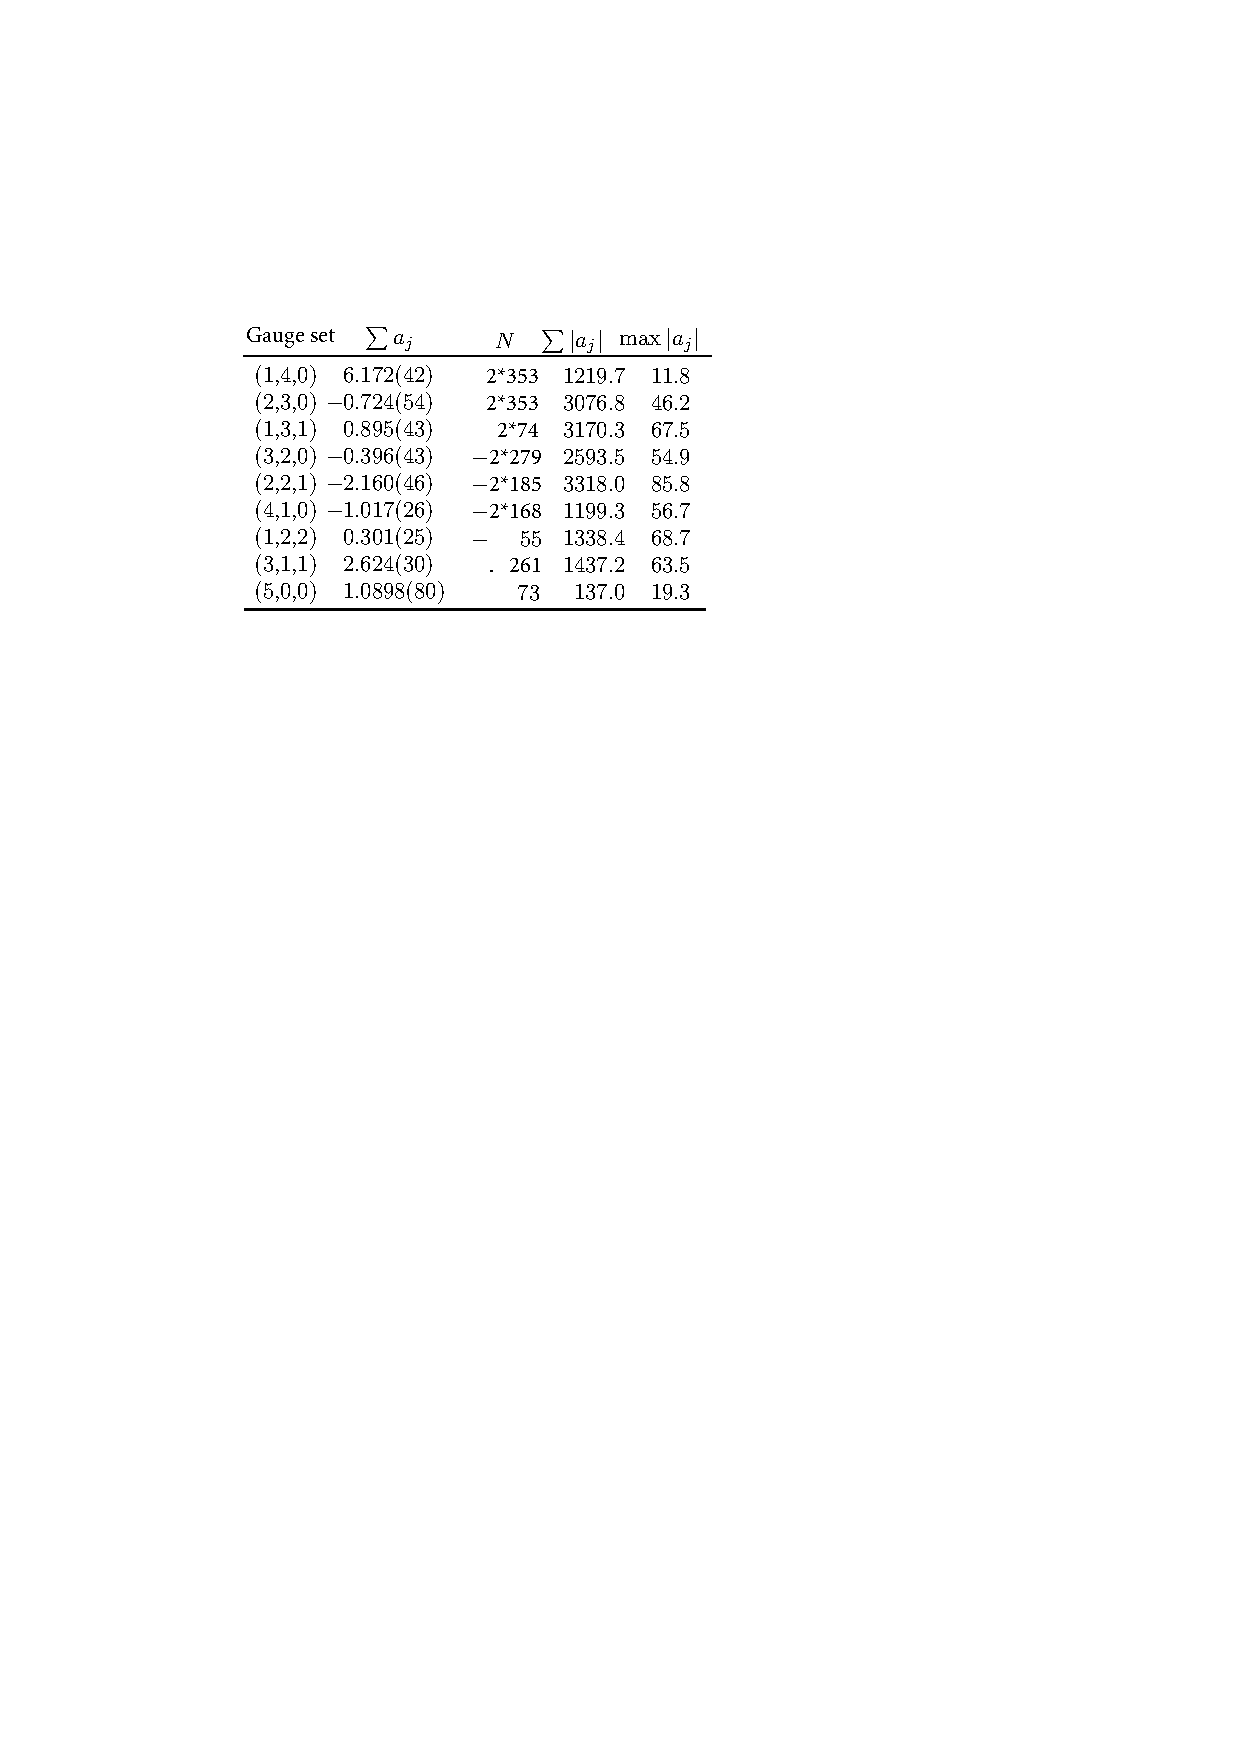
\includegraphics[width=0.60\textwidth]{Volkov19Tab1}
\end{center}
\caption{\label{Volkov19Tab1}
Contributions of the quenched QED $a^{(10)}[s]$ gauge sets, $s=(k,m,m')$.
If $m\neq m'$, the sum over $(k,m,m')+(k,m',m)$ is given, and the number
of contributing graphs is $2N_s$. Ignore the minus signs in $N$ column, a
PDF bug; I have also probably gotten the numbers of diagrams wrong.
Extracted from Volkov\rf{Volkov19} Table~1.
}
\end{table}
%%%%%%%%%%%%%%%%%%%%%%%%%%%%%%%%%%%%%%%%%%%%%%%%%%%%%%%%%%%

\item[2019-05-26 Predrag]
Volkov's
5-loop quenched QED gauge sets, are summarized in \reftab{Volkov19Tab1}.
Looking at the 4- and 5-loop results in \reftab{tabGaugeSets}, Volvkov surmises
that $(1,m,0)$ is approximately the final value, and the other values are
approximately zero with random errors (see {\bf 2018-12-21 Sergey} above).
However, gauge-set values surely do not look random to me; all signs except two
close to 0 follow my prediction, and the values are (unexplained) integers
multiples of 1/2.

Naive assumption would be that values of graphs contributing to gauge set
$s=(k,m,m')$ (do it separately from $s=(k,m',m)$ if $m\neq m'$) are uncorrelated
and randomly distributed, in which case one should test the randomness hypothesis by
computing the \emph{variance}
\beq
\expct{a^2_j}_{s} = \frac{1}{N_s}\sum_{j \in s} a^2_j
%\,.
\ee{variance_a_j}
for all gauge sets $s$ in \reftab{tabGaugeSets}, rather than listing $\sum
|a_j|$, as in Volkov's \reftab{Volkov19Tab1}, or my suggestion
\refeq{Volkov18AverMagn} above.
My interpretation of Volkov's $N_{diag}$ is likely wrong, as he writes that
``diagrams that are obtained from each other by changing arrow directions are
regarded as one,'' but that is easily fixed. It already seems that
$(5,0,0)$ and $(1,4,0)$ will be outliers.

More precisely, the {variance} is $\sigma^2=\expct{(a_j-\expct{a_j})^2}$,
and its positive square root is the \emph{standard deviation} $\sigma$.
This number depends on the gauge, and on particular auhtor's UV and IR
counter-term conventions, so it's hard to know what to make of it, but
getting a similar variance for all gauge sets would be cute.

\item[2019-06-04 Makiko Nio and Predrag to Sergey and Stefano] We have
looked together at the status of the 5-loop quenched QED, and what to do
to nail down the $4.5 \sigma$ difference between the two calculations.
Makiko's hunch is that the problem might be numerical, originating in a
Monte Carlo integral with a PDF defined in Seergey's \arXiv{1905.08007}
eq.~(1).

It looks to me that the ball is in Makiko's court; only way to compare is
via vertex diagram gauge sets, and she can do it if she really has to.

The first to check is $(5,0,0)$, both because it has the fewest diagrams,
and also because it is cleanest in terms of UV and IR counter terms. If
we ever manage to define and compute with a ``$k$-photon'' propagator,
$(k,0,0)$ has only one of them. Note also that max$|a_j|\approx 20$,
anomalously small.

$(1,4,0)$ (and the $(1,k,0)$ family of gauge sets) is fascinatingly
large. Our guess it that it might have to do with IR behaviour of the
4-loop self-energy insertion - Sergey can tell if there is something
going on there by looking at the contributing diagrams.
Note also that max$|a_j|\approx 10$, even more anomalously small, typical
size for the remaining gauge sets is max$|a_j|\approx 70$.

Next to knock off is $(1,2,2)$, then $(3,2,0)$. In my $1/2$ units I would
like to think of this set as well as $(2,2,0)$ as being approximately zero
(not to violate my gauge set sign rule).

\item[2019-09-19 Sergey] See Volkov\rf{Volkov19b} {\em }

\item[022-03-02 Sergey] See Volkov\rf{Volkov21}
{\em A way of fast calculating lepton magnetic moments in
Quantum Electrodynamics}

\item[2022-03-02 Sergey] See Volkov\rf{Volkov22}
{\em A flexible divergence elimination method for calculating
lepton magnetic moments in {Quantum Electrodynamics}}.
In principle I should check whether this is the same or different from
my methods...


\newpage
\item[2017-06-11 Predrag] to
\\
%Professor
Christian Schubert <schubert@ifm.umich.mx>
%\\
%Instituto de Física y Matem{\'a}ticas,\\
%Universidad Michoacana de San Nicol{\'a}s de Hidalgo,\\
%Ciudad Universitaria, C-3, Apdo. 2-82,\\
%C.P. 58040 Morelia, Michoacan, MEXICO
%
%\bigskip
%
%Dear Christian

Stefano Laporta  has recently published analytic values of all 4-loop
electron magnetic moment gauge sets, and they look very intriguing.
Sergey  A. Volkov has started evaluating individual 5-loop vertex
diagrams and is in position to estimate numerically the size of 5-loop
gauge sets. So it might be a good time to make a new attempt to prove/disprove
the QED finiteness conjecture. This set of notes is my current best attempt
to motivate this effort.

I do not take my 1977 ``gauge-set approximation'' very literally - its
content is only that if individual gauge sets can be bounded to anything
growing slower than combinatorially, quenched QED (and hopefully full
QED) is a finite theory, not an asymptotic series. But the form of vertex
gauge sets is very suggestive; it is defined in terms of $N$-photon
exchanges. So to me the wordline formalism seem the most promising way
forward.

While the quenched QED magnetic moment of electron is the cleanest
possible physical calculation one can do, for sociological reasons most
effort on high order estimates has gone in other directions. Do you have
a formula for spinor QED magnetic moment that one could attempt to
analyze more closely?

%As I have returned to this problem only last month, after a 40 year
%hiatus :) I would be grateful for any further pointers to the literature.

\item[2017-06-12 Christian]
I have been
fascinated by the finiteness conjecture ever after Gerald Dunne and I
were led there, too, from Euler-Heisenberg, Borel analysis,
Ritus mass shift and worldline instantons fifteen years ago.
The things have picked up a lot
just during the last year or so, namely:

\begin{enumerate}
  \item
Idrish Huet, Michel Rausch and I are working on the Affleck,
Alvarez and Manton (AAM) exponentiation conjecture\rf{AffAlMa82} in 1+1 QED.
We had a nice parameter integral representation for the three-loop
Euler-Heisenberg for quite a while, but could not get a sufficient number
of weak-field expansion coeffs out of it (so far what we got points to
AAM not holding at three loops - rather the coeffs go asymptotically
BELOW the AAM prediction - but this is very preliminary). Michel was just
visiting, and we now got a really nice algorithm (based on the polynomial
invariants of the dihedral group) for the analytical calculation of the
coeffs from the more difficult (nonplanar) 3-loop EH diagram.
  \item
If AAM really fails, then presumably the AAM worldline instanton needs
refinement at higher loops. My former student Naser Ahmadiniaz (now
postdoc in Korea) has made some progress with this.
  \item
For many years I am planning to apply the worldline formalism to (g-2),
in particular to the important graphs with the
light-by-light subdiagram. For this subdiagram I have, since a long time,
an off-shell representation that is permutation symmetric, manifestly
gauge invariant, without spurious UV poles, and moreover allows one to
trivially integrate out the one low-energy photon leg. What held me back
was that the various worldline representations that existed hitherto for
the electron line were all somewhat cumbersome, and seemed not suitable
for high-order calculations. Precisely this problem we have been working
on here for the last half year, and things have fallen into place really
nicely, we have a Bern-Kosower type master formula for the electron line
dressed with any number of photons, in vacuum and in the presence of a
constant field, and one of our students is already programming it. I am
now definitely trying to assemble a collaboration to attack the QED (g-2),
and I anticipate that your notes will be quite useful for motivating my
collaborators.

\end{enumerate}
Gies \etal\rf{GiSaVa05} have some intriguing numerical results from
worldline Monte Carlo (in section 5). Another thing I find quite
interesting are Ritus\rf{Ritus80} most recent
papers\rf{Ritus06,Ritus13,Ritus15} on the value of the bare fine
structure constant - he confirmed to me in an email from last December
(at age 90) that he definitely does not think that the bare charge is
infinite.

I am appending a summary of our efforts in this line of work\rf{HuTrSc17a}
which I wrote as a contribution to the 5th Winter Workshop on
Non-Perturbative Quantum Field Theory. 22-24 March 2017,
Sophia-Antipolis.

\item[2016-12-18 Vladimir I. Ritus] <v\_i\_ritus@mail.ru>
to Christian:

Thank you for your note about the papers by Johnson, Baker, Willey (Phys.
Rev. 1967, 1969, 1971) and by Adler, Bardeen (Phys. Rev. 1971).
    \PC{2017-08-04
    K. Johnson, M. Baker, and R. Willey, Phys. Rev. 136, B1111 (1964);
    ibid. 163, 1699 (1967); and
    S. L. Adler and W. A. Bardeen, Phys. Rev. D 4, 3045 (1971)
    These papers are about the possibility of the existence of an
    ultraviolet fixed point $\alpha_c$.
    }
I forgot them while writing my papers\rf{Ritus13,Ritus15}. Some months
ago I accidently saw  the abstracts of these papers in one of my
notebooks  with conspectus of the literature. Johnson et al assertion
confirms qualitatively my geometric and holographic duality approach to
the problem. Both of them deal with photons without self-energy
insertions. Have you any objections to this approach?

Nobody believes in infinite bare charge neither with space distribution
more singular than $\delta(x)$ nor as Landau pole at final transfer
momentum. Please, reed the several first phases in JRLR-paper (changing
the ``emitted"  to ``emitting").

I regret that I could not come to Tomsk, where I was at war time
1941-1943 in evacuation.

\item[2017-06-14 Christian to Ritus]
Just to make sure that I understand your conjecture correctly - are you
claiming that $1/4\pi$ is the value of the bare constant in the quenched
approximation, or in the full QED?

\item[2017-06-29 Vladimir Ritus]
The $1/4\pi$  is the value of the bare fine structure constant in the
full QED. It follows from duality of 4-dimensional QED and 2-dimensional
quantum field theory. The point charge moves  along timelike trajectory,
hence it has nonzero mass, but the photons emitted to infinity by this
charge are massless as the duality connected with them scalar quanta of
pairs emitted by the pointlike mirror in (1+1)-space. Constants
$\alpha_L$ and $\alpha_B$ are also geometrical. So, this theory is pure
geometrical and connected neither with the divergent perturbation theory
series, nor with the different methods of their summing. Please, read
\refrefs{Ritus13,Ritus15}.



\item[2017-06-18 Naser Ahmadiniaz] <ahmadiniaz.naser@gmail.com>
(currently a postdoctoral fellow at the Center for Relativistic Laser
Science (CoReLS), Institute for Basic Science (IBS), Gwangju, South
Korea).
\\
My main research
interests are in amplitude calculations in QED, QCD and quantum gravity
from the worldline formalism. Recently, we have been interested in
(off-shell) tree-level amplitudes for QED processes in vacuum as well as
in the presence of classical background fields which will also be applied
to higher order corrections.

\item[2017-06-20 James P. Edwards] <jedwards@ifm.umich.mx>,
%Instituto de Física y Matemáticas
%Universidad Michoacana de San Nicolás de Hidalgo
\HREF{www.ifm.umich.mx/ifm/index.php/fisca/academicos/edwards/}
{homepage}:
\\
I am currently working with Christian on the worldline approach. In some
of our recent work we have been working on more efficient ways to
determine g-2 based upon a worldline expression for the dressed spinor
propagator (both in vacuum and in a constant background).

\item[2017-06-11 Predrag] to
%\\
% Professor
Dirk Kreimer <kreimer@physik.hu-berlin.de>
%\\
%Humboldt-Universit\"at zu Berlin\\
%Institut f\"r Mathematik\\
%\bigskip
%
%Dear Dirk
%
%\medskip

Stefano Laporta  has recently published analytic values of all 4-loop
electron magnetic moment gauge sets, and they look very intriguing.
It might be a good time to make a new attempt to prove/disprove
the QED finiteness conjecture. This set of notes is my current best attempt
to motivate this effort.

If individual gauge sets can be bounded to anything growing slower than
combinatorially, quenched QED (and hopefully full QED) is a finite
theory, not an asymptotic series. The form of vertex gauge sets is
suggestive of a way forward; it is defined in terms of $N$-photon
exchanges. Hopf algebras might hold the key, but I do not know how to use
these ideas.

I would be grateful for any further pointers to the literature.
Anybody else I should send these notes to? And I'm
finally ready to stand up an be counted - I can fly to Berlin on a short
notice if that helps.

%\bigskip
%
%\noindent
%best regards
%\\
%Predrag
%\newpage

\item[2017-06-14 Dirk Kreimer] was kind enough to invite me to
\HREF{http://www2.mathematik.hu-berlin.de/~kreimer/wp-content/uploads/houches2018.html}
{Les Houches — June 4-15, 2018} on structures in local quantum field
theory. Edwards and I went, and learned a whole lot.

\item[2019-06-03 Christian Schubert and James P. Edwards]
We are still making sense of our master formulae but things are falling
into place. Our worldline efforts still are not paying off - a whole
class of terms that we had thought would not contribute on-shell for the
open fermion line actually does, And there is still the question whether
$g-2$ should be calculated in x-space or in p-space on the worldline
$\dots$ . We will keep you updated.

\item[2020-06-04 Somdatta Bhattacharya] <somdatta.bhattacharya@gmail.com>
writes: ``
I am intrigued by something you're an expert on. Soft photons correct the
QED vertex, so why don't they also affect $F_2(0)$ by a finite amount?
''
\\
{\bf Predrag} Dear Somdatta, \emph{you} are the expert\rf{Bhattacharya17}
:) Soft photons (were there an unambiguous gauge-invariant definition
that included both the IR divergences and the finite parts) contribute to
all radiative QED corrections, so surely they contribute to $g-2$
anomaly.

Here is my 5 cents. It's hand-waving, so I only say it in the privacy
of my QFT class - if you can turn it into mathematics, I would be grateful.

For me the IR and UV divergences exist on the same footing, even
cancelling each other\rf{MassShell}. However, the anomaly
\refeq{IRstruct(1)Q} does not have either\rf{IRstruct}. Why?

$F_2(0)$ part of the QED vertex form factor corresponds to flipping
the electron spin; soft photon cannot do that, that's why there is no
IR divergence. When you look at the parametric form of the
integral for $a_{0}^{(2)}$ it looks like the dominant contribution
is halfway where the infrared and ultraviolet singularities
would have been. So in my book, the soft photons are about 50\%
of the $F_2(0)$ anomaly.

PS If you actually read {\em Infra-red structure of {Yang-Mills}
theories}\rf{IRstruct}, it is not a stupid paper. That's why is has
garnered the total of 14 citations. I would be grateful for any earlier
(or later) reference that does it better or explains it more clearly.

PPS Maybe I should read
Fleischer and Tarasov\rf{FleTar92}
{\em Gauge-invariant on-shell {$Z_1$} in {QED} and {QCD}}?
(I do not have access to it online)

\item[2020-06-04 Somdatta Bhattacharya]
Here's my argument for why the $F_2(0)$ is zero at least up to first order,
but I end with a conundrum.

The amplitude for the vertex with the soft photon is akin to the Compton
scattering amplitude, with one of the photons being the soft one and the
other being the one of the vertex. In the limit of small photon momenta,
it is proportional to
$\overline{u}(p'.e/p'.k - p.e/p.k)\gamma^mu$
sandwiched
between the electron spinor states, where p' and p are the electron
momenta and k is the soft-photon one, e being the soft photon
polarization.

In the usual analysis, when you sum over polarizations and integrate for
the invariant momentum measure for k over the square of the expression
you get the Sudakov double logs in the scattering amplitude, that cancel
a similar expression coming from the loops, that is the $F_1$. I am
following Peskin and Schroeder.

Notice that the expression for the soft photons is exact, so that is all
that is there to it, and hence it doesn't give any contribution to
$F_2(0)$.

However, here's something interesting.

You get $(p'.e/p'.k-p.e/p.k)$ by acting with the Dirac operators on
specific spinors on either side of the Compton amplitude. But what if you
exchange p' and p by using momentum conservation and make the
corresponding Dirac operators act on the spinors on opposite sides. You
would get a totally different expression, involving
$[(p'.)/p'.k-(p.)/p.k](\gamma.e)$.
Now, ``in principle" such an expression ought to be
re-expressible in terms of
\(
\sigma. q.e. (F_2(p,p',k)) + \gamma.e(F_1(p,p',k))
\)
for some $F_2$ and $F_1$. The dots in the subscripts stand for greek
indices in the sigma expression.

And when squared and integrated over would give rise to a Rosenbluth-like
formula for electron scattering when one does the integral over k, from
which one can extract the ``effective" F's. Then setting the q to zero,
one should get the $F_2(0)$. Notice that like the $F_1$, this too would be
possibly divergent.

The only trouble is the finite q expressions should match with the result
computed using $(p'.e/p'.k - p.e/p.k)$, which gives just an $F_1$. But
this can't be possible, but I can't figure out the mistake in the naive
analysis. This is the conundrum I was referring to.

This is all I have come up with till now.

Here's something you might find of interest: \\
\emph{alternative worldline new.pdf} ;\;
\emph{SM from GR.pdf} \,.

Here's a rough draft I have written on new ways of doing QED one-loop calculations and their advantages. It's meant to open up discussions/collaboration:
\emph{QED new.pdf}.
Please take a look and let me know what you feel.

\item[2022-12-30 Christian Schubert]
Vladimir Ritus seems to be very anxious to have your opinion on
his papers about the calculation of alpha.

\item[2023-04-10 Sergey] sergey.volkov.1811@gmail.com \\
    Did you try to extend gauge-invariant classes beyond QED towards EW? For
    example, to take into account the difference between left and right
    electrons?
\item[2023-04-10 Predrag]
No, I did not.

The only new thing I have been thinking about is whether there is a
gauge-invariant planar field theory (the papers are
\HREF{ChaosBook.org/~predrag/papers/preprints.html\#PlanFieldThe} {here}) version of
QED. That would give a new, perturbatively convergent approximation to
QED. Lauwers, Scharbach and I had worked it out for QCD, in particular the
Ward identities  (7.17), but I do not remember why we did not apply it to
QED, which should be a simpler, special case.

I do not know if you know, but Kinoshita died recently. A very remarkable
man. I'll try to rework the notes I sent to you a long time ago as a paper in
his memory.


\end{description}

\newpage
% GitHub cvitanov/reducesymm/QFT/exponThe.tex
% to compile:  cd cvitanov/reducesymm/QFT; pdflatex blog; biber blog

% Predrag  created              Dec 23 2018

\section{Non-Abelian exponentiation theorem}
\label{s:FiMaFu18}
\newcommand{\vev}[1]{{\left< {#1} \right>}}

{\bf [2018-12-22 Predrag]}
% Bartomeu Fiol <bfiol@ub.edu>,  jmartinez@icc.ub.edu, ariosfukelman@icc.ub.edu
Fiol, Martínez-Montoya and Fukelman\rf{FiMaFu18} {\em Wilson loops in
terms of color invariants} address the question of whether one can
compute directly the logarithm of $\vev{W}_R$, the vacuum expectation
value (vev) of the Wilson loop.

The reason I'm intrigued by this paper is that their `$n$-gluon chord
diagrams' are also the no-fermion loop diagrams, or `quenched-'
% , or `q-type'
diagrams
% (`quenched', as this corresponds to the $N_f$-independent part
% of the vertex amplitude in QED with $N_f$ flavors)
of the quenched QED in
the worldline formalism. So far we are looking at what corresponds to
$\vev{W}_R$ chord diagrams, but we should really be looking at the $\ln
\vev{W}_R$ connected diagrams, and really at their Legendre transform,
the 1pI diagrams.

Their \emph{non-Abelian exponentiation theorem} implies that certain color
invariants present in $\vev{W}_R$ are absent in $\ln \vev{W}_R$.
To me this looks like the connection between the full and connected
partition functions, except that here quark lines are not providing
connections, only the crossed gluon lines are.

The color invariants $d_R^{a_1 a_1\dots a_k a_k}$ in (\ref{introexact})
can be reduced to lower order color invariants. This expansion is simpler
for $\ln \vev{W}_R$ than for $\vev{W}_R$ itself: the only color
invariants that appear in the perturbative expansion of $\ln \vev{W}_R$
at a given order are those that cannot be written as products of color
invariants that appear at lower orders of the perturbative expansion,
thus providing an illustration of the non-Abelian exponentiation theorem.

The theorem offer some support to the conjecture of
Fiol, Gerchkovitz and Komargodski\rf{FiGeKo16}
{\em Exact bremsstrahlung function in {N}=2 superconformal field theories}.

Only a subset of the most general color invariants appears in the
expansion of the bremsstrahlung function $B$.

The perturbative expansion of vevs can then be written in terms of
color invariants built from contractions of the
fully symmetrized traces
\beq
d_R^{a_1\dots a_n}
  =\frac{1}{n!} \sum_{\sigma \in {\cal S}_n} \hbox{ tr }
        T_R^{a_{\sigma(1)}}\dots T_R^{a_{\sigma (n)}}
\ee{symtraces}
where $T^a_R$ are the generators of the Lie algebra of the group G, in
the representation R.
$d_R$ with no indices is the trace of the identity matrix,
$d_R= \text {\tr} \, {\bf 1}= \text{dim } R$.
Some
examples of color invariants are $d_R^{aabb}$ or $d_R^{abcd}d_A^{abcd}$.

Fiol \etal\rf{FiMaFu18} conventions for color invariants are largely
those of van Ritbergen, Schellekens and Vermaseren {\em Group theory
factors for {Feynman} diagrams}\rf{RiScVe99},
\arXiv{hep-ph/9802376}.
Some of the invariants are given by Okubo and Patera {\em General indices
of simple {Lie} algebras and symmetrized product
representations}\rf{OkuPat83}. Many are presumably in Chaper~7 of
\refref{PCgr} and some in \refref{NPB81}; perhaps re-expressing color
invariants in terms of orthogonal Dynkin indices might yield some extra
insights.

They show that the vev of $W_R$ can be written in term of symmetrized
traces (\ref{symtraces}),
with pairwise contracted indices,
\beq
\vev{W}_R = \frac{1}{d_R}\sum_{k=0}^\infty \frac{1}{k!}
d_R^{a_1 a_1\dots a_k a_k} g^k
\,,
\ee{introexact}
where $g=g^2_\text{YM}/4$ is a Yang-Mills ``fine structure'' constant,
up to $\pi$ here and there.
This expression gives the vev of 1/2 BPS circular Wilson loop for any
representation R of a gauge group G. It allows to discuss exact relations
among vevs in different representations. For instance, if $R^t$ is the
transpose representation of $R$ (in the sense of having Young diagrams
transpose to each other), then, following \refrefs{NegDimE7,CK82,PCgr}
\[
\vev{W}_{R^t}(\lambda,N)=\vev{W}_R(\lambda,-N)
\]
thus relating, for instance, vevs in the symmetric and the antisymmetric
representations of \SUn{n}.

They carry out the integrals over the full Lie algebra
(in ${\cal N}=4$ super Yang Mills matrix model),
\beq
\vev{W}_R = \frac{1}{d_R}\vev{\hbox{\tr} \, e^{2\pi M}}=
 \frac{1}{d_R} \frac{\int_{\mathfrak{g}} dM    \,
\text{\tr} e^{2\pi M} \,
e^{-\frac{2\pi^2}{g}\text{tr }M^2}}{\int_{\mathfrak{g}}dM \,
e^{-\frac{2\pi^2}{g}\text{tr }M^2}}
\ee{winmm}
Denoting by $m^a$ the coefficients of the matrix $M$ in the Lie algebra,
the two-point function in this Gaussian matrix model is
\beq
\vev{m^a m^b}= \frac{g}{2\pi^2}\,\delta^{ab} \hspace{1cm} a,b=1,\dots, N
\ee{atwopoint}
To compute the vev of the normalized Wilson loop, we expand the exponent
insertion in (\ref{winmm}), use the two-point function (\ref{atwopoint})
and apply Wick's theorem,
\beq
\vev{W}_R =\frac{1}{d_R}\sum_{k=0}^\infty
\frac{(2\pi)^{2k}}{(2k)!} \vev{m^{a_1}\dots m^{a_{2k}}} \hbox{tr } T^{a_1}_R \dots T^{a_{2k}}_R=\frac{1}{d_R}\sum_{k=0}^\infty d_R^{a_1a_1\dots a_k a_k} \frac{g^k}{k!}
\ee{exactvev}
where $d_R^{a_1\dots a_k}$ are the symmetrized
traces (\ref{symtraces}).

At every order evaluation of the fully symmetrized traces
(\ref{symtraces}) with pairwise contracted indices $d_R^{a_1 a_1\dots a_k
a_k}$. yields a combination of lower order color invariants. At low
orders they evaluate them by hand, using the methods of van Ritbergen,
Schellekens and Vermaseren\rf{RiScVe99},
\begin{align*}
d_R^{aa} & =  \text{tr } T_R^a T_R^a= c_R d_R \\
d_R^{aabb} & =  \frac{1}{3}\text{ tr}
\left(2T_R^aT_R^aT_R^bT_R^b+T_R^aT_R^bT_R^aT_R^b\right)
=(c_R^2-\frac{1}{6}c_A c_R)d_R
\end{align*}
Higher orders, up to order $g^{7}$, they evaluate using
FormTracer\rf{CyMiSt16}. They are not pretty, but the perturbative
expansion of $\ln \vev{W}_R$ is considerably simpler.

For \SUn{n} fully (anti)symmetric irrep
there is an intriguing factorization, their eq.~(2.11).

Apparently one can write the power series for the logarithm of
$\vev{W}_R$ in terms of partial Bell polynomials $B_{n,k}$ (I do not
remember this formula). Defining $f_k=d_R^{a_1a_1\dots a_k a_k}/N_R$
\beq
\ln \vev{W}_R =\sum_{k=1}^\infty \frac{g^k}{k!}\sum_{j=1}^k
               (-1)^{j-1} (j-1)! B_{k,j}(f_1,f_2,\dots,f_{k-j+1})
\ee{logwbell}
A closed formula for the bremsstrahlung function follows, in terms of a
derivative with the respect to the coupling,
\beq
B_R(\lambda,N)
=\frac{1}{2\pi^2}\lambda \frac{\partial \ln \vev{W}_R}{\partial \lambda}
= \cdots
\ee{closedb}
This is worth remembering when thinking of the self-energy vs. vertex
diagram computation of the anomalous magnetic moment.

Expression (\ref{logwbell}) for $\ln \vev{W}_R$ is extremely inefficient,
and obscures the fact that the perturbative expansion of $\ln \vev{W}_R$
is simpler than that of $\vev{W}_R$. Computation of $\ln \vev{W}_R$ up to
order $g^{7}$ demonstrates that.
Many color invariants present in the expansion of $\vev{W}_R$ are absent
in the expansion of $\ln \vev{W}_R$. For instance, there are no color
invariants involving the quadratic casimir $c_R^k$ with $k\geq 2$. They
assert that this
simpler structure is a consequence of the non-Abelian exponentiation
theorem%\cite{Gatheral:1983cz, Frenkel:1984pz}:
; at every order in
perturbation theory, the only color invariants that can appear in $\ln
\vev{W}_R$ are the ones that cannot be written as products of color
invariants that appear at lower orders in the perturbative expansion of
$\vev{W}_R$.

Very interesting is their diagrammatic interpretation of the perturbative
expansion of $\ln \vev{W}_R$. According to the literature,
in the Feynman gauge, the only Feynman diagrams that contribute to
$\vev{W}_R$ involve gluon propagators starting and ending on the Wilson
line. Such diagrams are called \emph{chord diagrams}. %\cite{Touchard}.
At order $2n$
there are $(2n-1)!!$ of them. On the other hand, by virtue of the
non-Abelian exponentiation theorem,
%  \cite{Gatheral:1983cz,Frenkel:1984pz},
to compute $\ln \vev{W}_R$ one only needs to take into
account a subset of them, the so-called \emph{connected chord diagrams}:
diagrams where all gluon lines overlap with some other gluon line, see
\reffig{f:FiMaFu181f}.

\begin{figure}
\centering
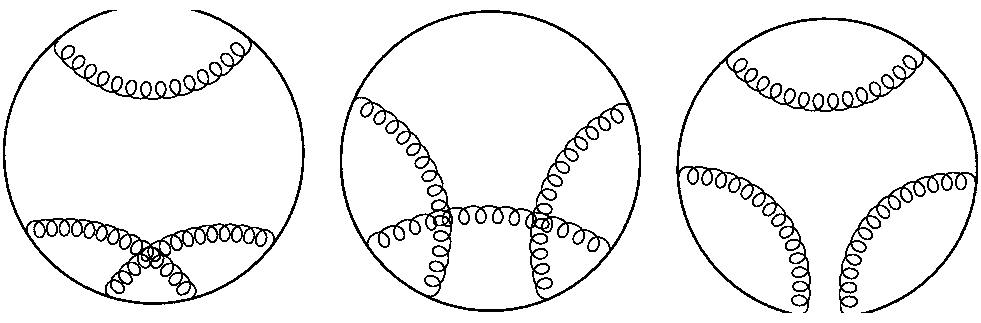
\includegraphics[width=.8\textwidth]{FiMaFu181f}
\caption{
Examples of chord diagrams. For $k$ gluons, by Wick's
theorem there are (2k-1)!! such diagrams. The second one is a connected
chord diagram. They contribute to $\ln \vev{W}_R$.
% Their number is given by the recursion relation (\ref{connectedchord}).
The last diagram is a
fully disconnected chord diagram.
For $k$ gluons, there are ${\cal C}_k= {(2k)!}/{(k+1)! k!}$ of them.
(From Fiol \etal\rf{FiMaFu18})
        }
\label{f:FiMaFu181f}
\end{figure}

The number of connected chord diagrams with $n$ chords satisfies the
recursion relation % \cite{stein, nijenwilf}
\beq
a_1=1 \hspace{1cm} a_n =(n-1)\sum_{k=1}^{n-1} a_k a_{n-k}
\,,
\ee{connectedchord}
so up to seven loops the numbers are
\[
a_n=1,1,4,27,248,2830,38232,\dots
\]
%It can be proven \cite{stein2} that
Asymptotically the ratio of the number of connected chord diagrams to the
total number of chord diagrams with $n$ gluons (or photons)
is $e$ times less than the total number of Feynman diagrams,
\[
\lim_{n\to \infty} \frac{a_n}{(2n-1)!!}=\frac{1}{e}
\,.
\]
To compute $\ln \vev{W}_R$ by evaluating just the connected gluon
diagrams, we have to take into account that according to the non-Abelian
exponentiation theorem,
% \cite{Gatheral:1983cz, Frenkel:1984pz},
the color factor of each diagram is a modified color factor $\bar c_i$.
To compute $\bar c_i$ of a given connected gluon diagram, one has
subtract the color factors of all possible gluon insertions of the diagram,
as illustrated in \reffig{f:FiMaFu18modCFac}.

\begin{figure}
  \centering
  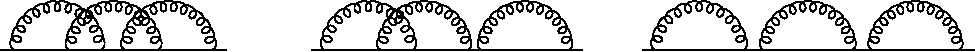
\includegraphics[width=1\textwidth]{FiMaFu18modCFac}
  \put(-263,2){\Large$-$\Huge$($}
  \put(-245,2){\LARGE$2$}
  \put(-132,2){\Large$+$}
  \put(0,2){\Huge$)$}
  \put(-290,-30){\large$\bar c= c_R \left( c_R - \frac{1}{2} c_A \right)^2 -  \left( 2c_R(-\frac{1}{2}c_R c_A)+c_R^3 \right)= \frac{1}{4} c_R c_A^3$}
  \caption{
The modified color factor of this connected 3-gluon diagram is obtained
by subtracting from its color factor all other gluon insertions.
(From Fiol \etal\rf{FiMaFu18})
    }
\label{f:FiMaFu18modCFac}
\end{figure}

Two chord diagrams have the same reduced color factor if their
intersection graphs are isomorphic. The intersection graph is defined as
follows: % \cite{Bouchet}:
for each chord introduce a point on the plane; if two chords cross, draw
an edge between the two points, see \reffig{f:FiMaFu186c}.
Since only connected chord diagrams contribute to $\ln \vev{W}_R$, we can
restrict our attention to connected intersection graphs. The numbers of
non-isomorphic connected intersection graphs for chord diagrams
% has been discussed in \cite{arratia}. Their numbers
are
\[
1,1,2,6,21,110,789,8336,117283,\dots
\]
At order $g^4$, there are $7!!=105$ 4-gluon chord diagrams, 27 connected
chord diagrams, and only 6 connected intersection graphs. In detail,
the 27 connected chord diagrams are grouped according to
six intersection graphs as $27=8+4+8+2+4+1$.
The reduced color factors that they list up to four loops, with
intersection graph up to four dots, are surprisingly simple.

\begin{figure}
\centering
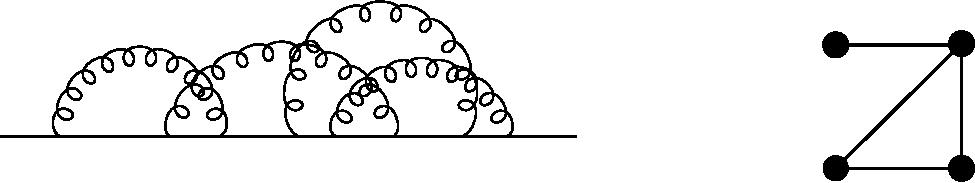
\includegraphics[width=.8\textwidth]{FiMaFu186c}
\caption{
The intersection graph of a 4-gluon Feynman diagram. For each gluon, draw
a dot on the plane; each time two gluon lines intersect, draw a link
between the corresponding dots.
(From Fiol \etal\rf{FiMaFu18})
    }
\label{f:FiMaFu186c}
\end{figure}

If $n$ is the number of gluon propagators, they have
\[
\ln \vev{W}_R= \sum_{n=1}^\infty \frac{1}{2n!}
\left(2 g^2\right)^n \sum_{conn} \bar c_i
\]
where the sum $\sum_{conn}$ runs over connected chord diagrams with $n$
gluon propagators.

Starting at seventh order, color invariants are not all independent; the
first identity they satisfy is\rf{RiScVe99}
\beq
d_A^{abcdef}d_A^{abcdef}-\frac{5}{8}d_A^{abcd}d_A^{cdef}d_A^{efab}
+\frac{7}{240}c_A^2 d_A^{abcd}d_A^{abcd}+\frac{1}{864}c_A^6 d_A
=0
\,.
\ee{adjointrelation}
They indulge in a bit of intriguing but so far inconclusive numerology.

\newpage
% reducesymm/QFT/finiteBlog.tex  compile by  pdflatex blog; bibtex blog
% $Author$ $Date$
% Predrag  switched to github.com               jul  8 2013

\section{QCD gauge sets - a blog}
\label{sect:QCDgaugeSets}

In 1981 Cvitanovi\'c \etal\rf{NPB81} constructed gauge invariant
subsectors in QCD.


\begin{description}

\item[2016-12-10 Predrag]
Penante\rf{Penante16} 2016 {{On-shell methods for off-shell quantities in N=4
Super Yang-Mills: from scattering amplitudes to form factors and the
dilatation operator}} has an up-to-date review of on-shell methods.

\item[2016-12-26 Predrag] Read
Cruz-Santiago, Kotko and Sta{\'s}to\rf{CrKoSt15} 2015
{\em Scattering amplitudes in the light-front formalism}:
``The idea is to divide the process into appropriate gauge invariant
components. It turns out that the gauge invariant subsets are invariant
under cyclic permutations of the external gluons. This decomposition was
proposed in works of [58–61] for the tree level amplitudes. A thorough
analysis of the relation between color structures and gauge invariance
was done in \refref{NPB81}. The color decomposition principle was
extended beyond the tree level to loop amplitudes in [63].''

\item[2016-12-26 Predrag]
Should also read Dixon\rf{Dixon96} 1996
{\em Calculating scattering amplitudes efficiently}.



\item[2017-05-26 Predrag]
The decomposition of scattering amplitudes into gauge invariant subsets
of diagrams is studied by Boos and Ohl\rf{BBLOM94,BooOhl99}.
Boos and Ohl\rf{BooOhl99}
{\em Minimal gauge invariant classes of tree diagrams in gauge theories},
\arXiv{hep-ph/9903357} (see \arXiv{hep-ph/9911437} and
\arXiv{hep-ph/0307057} for more detail) is motivated by applications to
Standard Model multi-particle diagrams, mostly at the tree level.

Perturbative calculations require an explicit breaking of gauge
invariance for technical reasons and the cancellation of unphysical
contributions is not manifest in intermediate stages of calculations. The
contribution of a particular Feynman diagram to a scattering amplitude
depends in the gauge fixing procedure and has no physical meaning.
the identification of partial sums of Feynman diagrams that are gauge
invariant by themselves is of great practical importance.
Calculation a subset of diagrams that is not gauge invariant has no
predictive power, because they depend on unphysical parameters introduced
during the gauge fixing.

A \emph{gauge invariance class} is a minimal subset of Feynman diagrams
that is independent of the gauge parameter and satisfies the
Slavnov-Taylor identities.

The set of diagrams connected by flavor and gauge flips they call
\emph{forest}, a set of diagrams connected by gauge flips the call
\emph{grove}. They shown that the groves are the minimal gauge invariance
classes of tree Feynman diagrams. In unbroken gauge theories, the
permutation symmetry of external gauge quantum numbers can be used to
subdivide the scattering amplitude corresponding to a grove further into
gauge invariant sub-amplitudes.

This (largely uncited) work seems to have no impact on the $(g-2)$
gauge sets discussed here.

\item[2017-05-27 Predrag]
Reuschle and Weinzierl\rf{ReuWei13} {\em Decomposition of one-loop {QCD}
amplitudes into primitive amplitudes based on shuffle relations}
cite our \refref{NPB81}. They say:

QCD calculations organise the computation of the one-loop amplitude as a sum
over smaller pieces, called \emph{primitive amplitudes}.
The most important features of a primitive amplitude are gauge invariance
and a fixed cyclic ordering of the external legs.
Primitive amplitudes should not be confused with \emph{partial amplitudes}
(also referred to as a \emph{dual amplitude} or a \emph{color-ordered amplitude}),
which are the kinematic coefficients of the independent colour
structures.
The first step in a discussion of perturbative Yang-Mills is the
decoupling of color from kinematics,
\beq
A_{tot} = \sum c_J A_J
\ee{KolShi14(1.1)}
where $A_{tot}$ represents the total amplitude for a scattering process,
$A_J $ are all the possible color structures,
and $A_J$ are partial amplitudes which depend only on the kinematical data
(momenta and polarizations).
Partial amplitudes are gauge invariant, but not
necessarily cyclic ordered.
Partial amplitudes are far simpler to calculate than the
full amplitude. There
exist linear relations among the partial amplitudes, called
Kleiss-Kuijf relations, which reduce the number of linearly
independent partial amplitudes to $(n-2)!$
The leading contributions in an $1/N$-expansion (with $N$ being the number of colours)
are usually cyclic ordered, the sub-leading parts are in general not.
The decomposition of the full one-loop amplitude into partial amplitudes is easily derived.
However, it is less trivial to find a decomposition of the partial
amplitudes into primitive amplitudes.

There are several possible choices for a basis in colour space.
A convenient choice is the colour-flow basis\rf{tHooft:1974jz}.

\item[2017-05-27 Predrag]
Schuster\rf{Schuster14} {\em Color ordering in {QCD}}: ``
We derive color decompositions of arbitrary tree and one-loop QCD
amplitudes into color-ordered objects called primitive amplitudes.
''

\item[2017-05-27 Predrag]
Zeppenfeld\rf{Zeppenfeld88}
{\em Diagonalization of color factors} (Georgia Tech has no access to this paper)

\item[2017-05-27 Predrag]
Edison and Naculich\rf{EdiNac12} {\em Symmetric-group decomposition
of {SU(N)} group-theory constraints on four-, five-, and six-point
color-ordered amplitudes at all loop orders}: ``
Color-ordered amplitudes for the scattering of n particles in the adjoint
representation of SU(N) gauge theory satisfy constraints that arise from
group theory alone. These constraints break into subsets associated with
irreducible representations of the symmetric group $S_n$, which allows
them to be presented in a compact and natural way.
''

\item[2017-05-27 Predrag]
Kol and Shir\rf{KolShi14,KolShi15}
{\em Color structures and permutations} has a
useful overview of the literature in the introduction, and is a very
interesting read overall.

We may permute (or re-label) the external legs in the expression for a
color structure and thereby obtain another color structure. This means
that the space of color structures is a representation of $S_n$, the
group of permutations. A natural question is to characterize this
representation including its character and its decomposition into
irreducible representations (irreps).

The decomposition of color structures into irreps was suggested by
Zeppenfeld\rf{Zeppenfeld88}.

The space of tree-level color structures $TCS_n$ of dimension
\beq
\mbox{dim}(TCS_n) = (n-2)!
\ee{KolShi14(2.7)}
is the vector space
generated by all diagrams with $n$ external legs and an oriented cubic
vertex, which are connected and without loops (trees), where diagrams
which differ by the Jacobi identity are to be identified.

The $f$-based and $t$-based color structures are related by celebrated
Kleiss-Kuijf\rf{KleKui89} relations (rederived in this paper).

The original problem, that of capturing symmetries of the partial
amplitudes which originate with those of the color structures, is now
formulated as the problem of obtaining the $S_n$ character
of the space of color structures. It turns out that (at least at
tree level) this problem was fully solved in the mathematics literature
by Getzler and M. M. Kapranov\rf{GetKap98}.

The free Lie algebra over some set $A$, denoted by $L(A)$, is the Lie
algebra generated by $A$ with no further relations apart for antisymmetry
and the Jacobi identity which are mandated by definition.

Self duality under Young conjugation: for some $n$ values $TCS_n$  is
self-dual under Young conjugation, namely under the interchange of rows
and columns in the Young diagrams

\item[2017-05-27 Predrag]
Getzler and Kapranov\rf{GetKap98} {\em Modular operads}: ``
We develop a `higher genus' analogue of operads, which we call modular
operads, in which graphs replace trees in the definition. We study a
functor $F$ on the category of modular operads, the Feynman transform,
which generalizes Kontsevich's graph complexes and also the bar
construction for operads. We calculate the Euler characteristic of the
Feynman transform, using the theory of symmetric functions: our formula
is modelled on Wick's theorem.
''

\item[2017-05-27 Predrag]
Maltoni \etal\rf{MPSW03}
{\em Color-flow decomposition of {QCD} amplitudes}

The \emph{color-flow} decomposition is based on treating the $SU(N)$
gluon field as an $N\!\times\!N$ matrix.
(PC: I think that is what I actually do.)
It has several nice features.
First, a similar decomposition exists for all multiparton amplitudes,
like the fundamental-representation decomposition. Second, the color-flow
decomposition allows for a very efficient calculation of multiparton
amplitudes. Third, it is a very natural way to decompose a QCD amplitude.
As the name suggests, it is based on the flow of color, so the
decomposition has a simple physical interpretation.

To calculate the amplitude, one orders the gluons clockwise, and draws
color-flow lines, with color flowing counterclockwise, connecting
adjacent gluons. One then deforms the color-flow lines in all possible
ways to form the Feynman diagrams that contribute to this partial
amplitude. The Feynman diagrams that contribute to a partial amplitude
are planar. This is not due to an expansion in $1/N$; the partial
amplitudes are exact. They note (see their Table 1) that the number of
Feynman diagrams contributing to an $n$-gluon partial amplitude grows as
$\approx 3 \cdot 8^n$. In contrast, the number of Feynman diagrams
contributing to the full amplitude grows factorially, as
$\approx (2n)!$.


%\item[2017-05-27 Predrag] in the spirit of Feynman's challenge,
%track the progeny o gauge sets
%
%(1,0,0) $\to$ (2,0,0) + ((1,1,0) + (1,0,1))
%
%(2,0,0) $\to$ (3,0,0) + ((2,1,0) + (2,0,1))
%
%((1,1,0) + (1,0,1)) $\to$ (1,1,1) + ((2,0,1) +  + (1,0,2))
%
%
%(1,1,0),
%
%(2,0,0)
%
%(1,0,1)

\item[2017-06-09 Predrag]
Henn \etal\rf{HLSSS17}
{\em Four-loop photon quark form factor and cusp anomalous dimension in
the large-{$N_c$} limit of {QCD}}, \arXiv{1612.04389}, is a thoroughly
modern paper, a listing of different codes used to generate diagrams and
evaluate integrals.

\item[2017-06-16 Predrag]
Chang, Liu and Roberts\rf{ChLiRo11}
{\em Dressed-quark anomalous magnetic moments}

\item[2017-06-16 Predrag]
Choudhury and Lahiri\rf{ChoLah15}
{\em Anomalous chromomagnetic moment of quarks}

\item[2017-06-16 Predrag]
Bermudez \etal\rf{BAGTB17}
{\em Quark-gluon vertex: {A} perturbation theory primer and beyond},
\arXiv{1702.04437}:
The on-shell limit enables us to compute anomalous chromomagnetic moment
of quarks.

[...] we present some ``physically" relevant results for
the on-shell limit $p^2=k^2=m^2$ and $q^2=0$. The Dirac and Pauli
form factors, $F_1(q^2)$ and $F_2(q^2)$, respectively, define the
Gordon decomposition of the quark current as in \refeq{BAGTB17(35-1)}.
The anomalous chromomagnetic moment (ACM) of quarks can be
identified as $F_2(q^2)$ for $q^2 \rightarrow 0$. The Abelian
version of this decomposition with $C_F=1$ and $C_A=0$ is the
electron-photon vertex of quantum electrodynamics. The great
successes of the Dirac equation is the prediction of the magnetic
moment of a charged fermion  ${ {\mu}} = {eg}/{(2 m)} { S}$.
The radiative corrections lead to\rf{Schwinger48}
 \bea
 \frac{e}{2 m} \Rightarrow \left( 1 + \frac{\alpha}{2 \pi} \right) \frac{e}{2
 m}.
 \eea
Note that the quark-gluon vertex differs from the electron-photon vertex
already at one loop, by the contributions of an additional Feynman
diagram, involving the triple-gluon vertex. In fact, apart from
introducing additional color structure, this non-Abelian diagram
introduces, at the one-loop level, a kinematical structure which is
absent in the QED.

It is straightforward to see that for the soft gluon limit, $q^2=0$, the
Abelian contribution for the ACM reduces to the non-Abelian counterpart
of Schwinger's result, $F_{2}^{a}(0) = - \alpha /12 \pi$, already derived
in \refref{ChLiRo11}. On the other hand, the corresponding non-Abelian
contribution yields a divergence\rf{ChoLah15}, for a non-zero quark mass,
$m \neq 0$. We find this divergence to be logarithmic. For deep infrared
gluon momenta it behaves as $F_2^{b}(q^2 \rightarrow 0)= C_b \ln \left( -
q^2/m^2 \right)$. Of course, perturbation theory in QCD is not the way to
explore deep infrared region. All perturbative conclusions will be taken
over by non-perturbative effects, overshadowing this divergence.

\item[2017-06-16 Predrag]
Brambilla \etal\rf{Brambilla14}
{\em {QCD} and strongly coupled gauge theories: challenges and perspectives}

\item[2017-06-16 Predrag]
Simonov and Tjon\rf{SimTjo02}
{\em The {Feynman–Schwinger} representation in {QCD}}:``
The proper time path integral representation is derived for Green's
functions in QCD. After an introductory analysis of perturbative
properties, the total gluonic field is separated into a nonperturbative
background and valence gluon part. For nonperturbative contributions the
background perturbation theory is used systematically, yielding two types
of expansions. As an application, we discuss the collinear singularities
in the Feynman–Schwinger representation formalism.
''



\end{description}

\newpage
\section{Is QED finite? A blog}
\label{sect:finiteBlog}

\begin{description}

\item[1950-12-22 Schwinger]
{\em On gauge invariance and vacuum polarization}\rf{Schwinger51c}
has 3700 citations.
He writes: ``
This paper is based on the elementary remark that the extraction of gauge
invariant results from a formally gauge invariant theory is ensured if
one employs methods of solution that involve only gauge covariant
quantities. We illustrate this statement in connection with the problem
of vacuum polarization by a prescribed electromagnetic field. The vacuum
current of a charged Dirac field, which can be expressed in terms of the
Green's function of that field, implies an addition to the action
integral of the electromagnetic field. Now these quantities can be
related to the dynamical properties of a ``particle" with space-time
coordinates that depend upon a proper-time parameter. The proper-time
equations of motion involve only electromagnetic field strengths, and
provide a suitable gauge invariant basis for treating problems. Rigorous
solutions of the equations of motion can be obtained for a constant
field, and for a plane wave field. A renormalization of field strength
and charge, applied to the modified lagrange function for constant
fields, yields a finite, gauge invariant result which implies nonlinear
properties for the electromagnetic field in the vacuum.
[...]
one can employ an expansion in powers of the potential vector. The latter
automatically yields gauge invariant results, provided only that the
proper-time integration is reserved to the last. This indicates that the
significant aspect of the proper-time method is its isolation of
divergences in integrals with respect to the proper-time parameter, which
is independent of the coordinate system and of the gauge. The connection
between the proper-time method and the technique of ``invariant
regularization" is discussed. Incidentally, the probability of actual
pair creation is obtained from the imaginary part of the electromagnetic
field action integral. Finally, as an application of the Green's function
for a constant field, we construct the mass operator of an electron in a
weak, homogeneous external field, and derive the additional spin magnetic
moment of $\alpha/2\pi$ magnetons by means of a perturbation calculation
in which proper-mass plays the customary role of energy.
''

``
A proper time wave equation, in conjunction with the second order
Dirac operator, has been discussed by
V. A. Fock\rf{Fock37}
{\em Proper time in classical and quantum mechanics}.
See also Nambu\rf{Nambu50} (1950).
''

In Appendix~B Schwinger computes the anomalous spin magnetic
moment $\alpha/2\pi$ produced by second-order electromagnetic mass effects.

\item[1977-03-03 Drell and Pagels]
{\em Anomalous magnetic moment of the electron, muon, and nucleon}\rf{DrePag65}
attempt got the sign right, but was not successful in predicting the
magnitude of the sixth-order magnetic moment;
$0.15 \left(\frac{\alpha}{\pi}\right)^3$ instead of
$1.19 \left(\frac{\alpha}{\pi}\right)^3$.

\item[1971-08-01 Lautrup, Peterman, and de Rafael]
 1972 {\em Recent
developments in the comparison between theory and experiments in quantum
electrodynamics}\rf{LaPeRa72} list the 3-loop, no-electron loop ``gauge invariant
subclasses'' (their Fig.~4.3).

\item[1974-01-07 Samuel]
1974 {\em Estimates of the eighth-order corrections
to the anomalous magnetic moment of the muon}\rf{Samuel74}:

``We speculate that in making radiative corrections to a class of graphs
by inserting a single photon in all possible ways, one obtains a
contribution which is roughly $-\frac{\alpha}{\pi}$ times the
contribution of the class. This seems to be obeyed by the known
contributions.''

\item[2013-11-24  Predrag]
As far as I can tell, terminology ``of \emph{quenched} type'' was first
introduced in this context by
Marinari, Parisi and Rebbi\rf{MaPaRe81}
{\em {Monte Carlo} simulation of the massive {Schwinger} model},
in the context of lattice gauge theory. They write:
``A first approximation to the effect of the gauge field on the fermion
observables may be achieved by [...] neglecting the contributions from
the fermionic vacuum polarization diagrams and, using a terminology
developed in the theory of condensed matter, we shall call the
expectation values thus obtained `quenched'",

Parisi is reputable, so in the ``quenched approximation" one neglects
the fermionic vacuum polarization effects (i.e, the fermion loops) from
the fermion determinant in the effective action. If it is good enough for Kinoshita,
it is good enough for you.

``In the ‘quenched approximation’ the quark determinant is set equal to
unity, i.e., neglecting the effect of virtual quark loops. In
other words, this extreme approximation in terms of heavy quarks with a
vanishing number of flavors assumes that gauge fields affect quarks while
quarks have no dynamical effect on gauge fields."

A more general usage: ``In Quantum Cosmology ‘‘quenching,’’ amounts to
quantizing a single scale factor thereby selecting a class of
cosmological models, for instance, the Friedmann-Robertson-Walker
space-time while neglecting the quantum fluctuations of the full
metric.''

But I still do not like it - it is mostly associated with Kogut, where it
means something different (as in ``... treating the gauge interaction in
the quenched, planar (ladder) approximation"); search for quench
\HREF{http://en.wikipedia.org/wiki/Quantum_chromodynamics} {here}. Or
here is what Brezin says:

``concept of quenching is well-known in the statistical mechanics of
random media ; consider a system of particles, for instance, an electron
gas, interacting with impurities. If these impurities are mobile, they
will thermalize with the electron gas and the average physical quantities
are obtained by a trace over the electron gas and the impurities degrees
of freedom. However if the impurities are frozen, the `quenched' case,
the physical observables are obtained by calculating their value for
fixed impurities and then averaging over these
impurities. "

That is how I know it - nothing about fermion loops, just dirt physics...

From my point of view, the question is whether the sum of all
corrections to (g-2) is a convergent series, or an asymptotic one.
If on can prove the convergence for the quenched sector, I would
expect each un-quenched sector (diagrams with one, two, .... lops)
separately to be convergent, and their sum as well.

Here is something to amuse you:
\HREF{http://www.scottaaronson.com/blog/?p=1537}{on amplituhedron}.
More serious: Lance Dixon
\HREF{http://www.preposterousuniverse.com/blog/2013/10/03/guest-post-lance-dixon-on-calculating-amplitudes/}
{on calculating amplitudes}.

The inventor of the ``gauge invariant diagram sets" concept is Benny
Lautrup.

\item[2013-12-08  Predrag] to Piotr, Wanda and Andrea
(Piotr Czerski <piotr.czerski@ifj.edu.pl>,
 wanda.alberico@to.infn.it,
 andrea.prunotto@gmail.com):

I'm no fan of Feynman diagrams (my rant is
\HREF{http://www.cns.gatech.edu/~predrag/papers/preprints.html\#FiniteFieldTheo}
{here}), and I'm always looking
for other ways to look at perturbative expansions. So just a little email
- if you have a new angle\rf{PrAlCz13} on subsets of diagrams which are gauge
invariant sets, I would be curious to learn how you look at that.

Just something to keep in mind :)

PS to Andrea: I realize you might rather forget this stuff (takes you a
decade to write a paper?) but at least I got a ringtone out of you. The
only problem is, I do not have a cell phone, so I do not know how to make
it ring. At least I'm more technologically savvy than
\HREF{http://www.theguardian.com/science/2013/dec/06/peter-higgs-boson-academic-system?CMP=twt_gu}
{Peter Higgs}.

\item[2013-12-10  \HREF{https://sites.google.com/site/andreaprunotto/} {Andrea}]
Sorry for late reply (well, we're used to longer gaps). Yes! I actually
took 10 years to write this paper out of my master thesis, but I have
some excuses: I did my PhD in Biochemistry (Z\"urich) and now I work on
genetics (Lausanne). This summer my ``old'' professor Wanda found my work
in a drawer and then contacted me, telling me that it would be a good
idea to publish it.

About your request: I'm really interested in seeing if the rooted-map
approach to Feynman diagrams can address the problem you've risen. But I
have no idea what the ''subsets of diagrams which are gauge invariant
sets'' are. I've checked a bit on the web but I'm sure you can give me
better indications (the works I found were too technical: I need to know
the basis of the problem). Can you send me some specific link at freshman
level, in particular where I can see the geometry of these subclasses of
diagrams?

\item[2013-12-11  Predrag]
Googling is good, but it is faster to click on
\HREF{http://www.cns.gatech.edu/~predrag/papers/preprints.html\#FiniteFieldTheo}
{this link}. The article defines the gauge invariant sets.

\item[2014-02-11 M. Borinsky]
\emph{Feynman graph generation and calculations in the Hopf algebra of
Feynman graphs}\rf{Borinsky14}
``Programs for the computation of perturbative expansions of quantum
field theory amplitudes are provided. feyngen can be used to generate
Feynman graphs for Yang-Mills, QED and $phi^k$ theories. feyncop
implements the Hopf algebra of those Feynman graphs which incorporates
the renormalization procedure necessary to calculate finite results in
perturbation theory of the underlying quantum field theory. ''

\item[2016-02-08  Predrag]
Prunotto\rf{Prunotto03}
{\em A Homological Approach to Feynman Diagrams in the Quantum Many-Body Theory},
and
Prunotto, Alberico and Czerski\rf{PrAlCz13} 2013
{\em Feynman Diagrams and Rooted Maps}
has been submitted to the European Physical Journal A as manuscript ID EPJA-103480,
seems not to have been published anywhere by 2017.
%I have been asked to referee it, but have declined - too busy.
They write: ``
The  Rooted Maps Theory, a branch of the Theory of Homology, is shown to be
a powerful tool for investigating  the topological properties of Feynman
diagrams, related to the single particle propagator in the quantum many-body
systems. The numerical correspondence between the number of this class of
Feynman diagrams as a function of perturbative order and the number of rooted
maps as a function of the number of edges is studied. A graphical procedure to
associate Feynman diagrams and rooted maps is then stated. Finally, starting
from rooted maps principles, an original definition of the genus of a
Feynman diagram, which totally differs from the usual one, is given.
''

\item[2017-03-15 Predrag]
Dunne and Krasnansky\rf{DunKra06} 2006 {\em ``Background field
integration-by-parts'' and the connection between one-loop and two-loop
{Heisenberg-Euler} effective actions}: ``
We develop integration-by-parts rules for diagrams involving massive
scalar propagators in a constant background electromagnetic field, and
use these to show that there is a simple diagrammatic interpretation of
mass renormalization in the two-loop scalar QED Heisenberg-Euler
effective action for a general constant background field. This explains
why the square of a one-loop term appears in the renormalized two-loop
Heisenberg-Euler effective action, and
dramatically simplifies the computation of the renormalized two-loop
effective action for scalar QED, and generalizes a previous result
obtained for self-dual background fields.
''

\item[2017-05-23 Predrag]
\phantomsection \label{sect:SchSch96}
M. G. Schmidt and C. Schubert\rf{SchSch96} 1994
{\em Multiloop calculations in the string-inspired formalism: the single
spinor-loop in QED}, \arXiv{hep-th/9410100}:
They use the worldline path-integral Bern-Kosower formalism
for to calculate the sum of all diagrams
with one spinor loop and fixed numbers of external and internal photons.
Of interest: in this formalism the three 2-loop photon polarization graphs,
see \reffig{BHSTW143loopphotonprop},
are a single integral, easier to evaluate than any of the three Feynman
graphs. They also note an unexplained cancelation not only of poles, but also
of ``transcedentals.''
A knot-theoretic explanation for the rationality of the quenched
QED beta function is given in \refref{BrDeKr96}.

\item[2017-05-23 Predrag]
Nieuwenhuis and Tjon\rf{NieTjo96} 1996
{\em Nonperturbative study of generalized ladder graphs in a {$\phi^2\chi$} theory},
\arXiv{hep-ph/9606403}:

\item[2017-05-23 Predrag]
Christian Schubert\rf{Schubert01} 2001
{\em Perturbative quantum field theory in the string-inspired formalism},
\arXiv{hep-th/0101036}:

The Feynman rules for (Euclidean) spinor QED in the second order
formalism (see Morgan\rf{Morgan95} 1995,
Strassler\rf{Strassler92} 1992, and references therein) are, up to
statistics and degrees of freedom, the ones for scalar QED with the
addition of a third vertex. % (Fig. 17).
The third vertex involves
$\sigma^{\mu\nu}={1\over 2}[\gamma^{\mu},\gamma^{\nu}]$
and corresponds to the $\psi^{\mu}F_{\mu\nu}\psi^{\nu}$
-- term in the worldline Lagrangian $L_{\rm spin}$.
%(compare eq.(\ref{Weucl})).
For the details and for the non-abelian case see Morgan\rf{Morgan95}.
There also an algorithm is given, based on the Gordon identity, which
transforms the sum of Feynman (momentum) integrals resulting from the
first order rules into the ones generated by the second order rules.

\item[2017-06-12 Predrag]
Morgan\rf{Morgan95}
{\em Second order fermions in gauge theories}, \arXiv{hep-ph/9502230}
seems to be the same discussion that I use in my QFT course to define the
electron magnetic moment via $\sigma^{\mu\nu}$ (see lectures 25 and 26
\HREF{http://chaosbook.org/~predrag/courses/PHYS-7147-13/schedule.xml}
{here})

\item[2017-06-12 Predrag]
Gies, Sanchez-Guillen, V{\'a}zquez\rf{GiSaVa05}
{\em Quantum effective actions from nonperturbative worldline dynamics},
 \arXiv{hep-th/0505275}: ``
We demonstrate the feasibility of a nonperturbative analysis of quantum
field theory in the worldline formalism with the help of an efficient
numerical algorithm. In particular, we compute the effective action for a
super-renormalizable field theory with cubic scalar interaction in four
dimensions in quenched approximation (small- N f expansion) to all orders
in the coupling. We observe that nonperturbative effects exert a strong
influence on the infrared behavior, rendering the massless limit well
defined in contrast to the perturbative expectation.
''

\item[2017-06-12 Predrag]
Giesand H{\"a}mmerling\rf{GieHam05}
{\em Geometry of spin-field coupling on the worldline},
\arXiv{hep-th/0505072}:

\item[2017-03-15 Predrag]
Huet, McKeon, and Schubert\rf{HuMcSc10} 2010
{\em {Euler-Heisenberg} lagrangians and asymptotic analysis in 1+1 {QED. Part I: Two}-loop}
(no GaTech online access, \arXiv{1010.5315}):``
We continue an effort to obtain information on the QED perturbation
series at high loop orders, and particularly on the issue of large
cancellations inside gauge invariant classes of graphs, using the example
of the l-loop N-photon amplitudes in the limit of large photon
numbers and low photon energies. The high-order
information on these amplitudes can be obtained from a nonperturbative
formula, due to Affleck \etal\rf{AffAlMa82}, for the imaginary part of the QED
effective lagrangian in a constant field. The procedure uses Borel
analysis and leads, under some plausible assumptions, to a number of
nontrivial predictions already at the three-loop level. Their direct
verification would require a calculation of this `Euler-Heisenberg
lagrangian' at three-loops, which seems presently out of reach
(though see Huet, de Traubenberg, and Schubert\rf{HuTrSc17} below). Motivated
by previous work by Dunne and Krasnansky\rf{DunKra06} on Euler-Heisenberg
Lagrangians in various dimensions, in the present work we initiate a new
line of attack on this problem by deriving and proving the analogous
predictions in the simpler setting of 1+1 dimensional QED. In the first
part of this series, we obtain a generalization of the formula of
Affleck \etal\rf{AffAlMa82}
to this case, and show that, for both scalar and spinor QED, it
correctly predicts the leading asymptotic behaviour of the weak field
expansion coefficients of the two loop Euler-Heisenberg lagrangians.

``The present work continues an
effort\rf{DunSch02I,DunSch02II,MaScVi03,DunSch06} to study the multiloop
behaviour of the QED $N$-photon amplitudes using the QED effective
lagrangian, and in particular to prove or disprove Cvitanovi\'c's
conjecture for these amplitudes.''

\item[2017-05-24 Predrag]
Bastianelli, Huet, Schubert, Thakur and Weber\rf{BHSTW14} 2014
{\em Integral representations combining ladders and crossed-ladders}
write:

This property is particularly interesting in view of the fact that it is
just this type of summation which in QED often leads to extensive
cancellations, and to final results which are substantially simpler than
intermediate ones (see, e.g., \refref{Cvit77b,BrDeKr96}). More recently, similar
cancellations have been found also for graviton amplitudes (see, e.g.,
\refref{BaBjVa09}).
Although this property of the worldline formalism is well-known, and has
been occasionally exploited\rf{rossch96a,rossch96b, SchSch96,BaRoSt06} (see also
\refref{FriGab12}) a systematic study of its implications is
presently still lacking.

The first classes of Green's functions %, depicted in fig. \ref{fig:Nprop},
is the
$x$-space propagator for one scalar interacting with the second one
through the exchange of $N$ given momenta.

This object, to be called ``$N$-propagator'', is given by a set of $N!$
simple tree-level graphs, is in the worldline formalism combined into a
single integral.

The second class are the similarly looking  $x$-space $N+2$ - point
functions %shown in fig \ref{fig:halfladder},
defined by a line connecting
the points $x$ and $y$ and $N$ further points $z_1,\ldots,z_N$ connecting
to this line in an arbitrary order.

An advantage of the worldline representation over the usual Feynman
parameterization is the automatic inclusion of all possible ways of
crossing the ``rungs'' of the ladders. They obtain such representations
in explicit form both in $x$-space and in momentum space.

The inclusion of the crossed ladder graphs is essential for the
consistency of the one-body limit where one of the constituents becomes
infinitely heavy, and for maintaining gauge invariance.

They concentrate on the case of infinite $N$, \hbox{\it i.e.}, the sum
over {\it all} ladder {\it and} crossed ladder graphs.

As their main application, they consider the case of two massive scalars
interacting through the exchange of a massless scalar, obtain an the case
of a massless exchanged particle (along the ``rungs'' of the ladders).

Applying
asymptotic estimates and a saddle-point approximation to the $N$-rung
ladder plus crossed ladder diagrams, they derive a semi-analytic
approximation formula for the lowest bound state mass in this model.

They use the worldline formalism to derive integral representations for
the $N$-propagators and the $N$-ladders - in scalar field theory,
and give a compact expression combining the $N!$ Feynman diagrams
contributing to the amplitude. They give these representations in both
$x$ and (off-shell) momentum space. Being off-shell, can be used
as building blocks for more complex amplitudes. They derive a
compact expression for the sum of all ladder graphs with $N$ rungs,
including all possible crossings of the rungs.

Nieuwenhuis and Tjon\rf{NieTjo96} 1996 have numerically evaluated the path
integrals of the worldline representation for the same scalar model field
theory, thus including all ladder {\it and}
crossed ladder graphs.

\item[2017-05-23 Predrag]
Huet, de Traubenberg, and Schubert\rf{HuTrSc17} 2017
{\em Multiloop {Euler-\,Heisenberg Lagrangians, Schwinger} pair creation,
and the photon {S-matrix}}:
``Schwinger pair creation in a constant electric field, may possibly
provide a window to high loop orders; simple non-perturbative closed-form
expressions have been conjectured for the pair creation rate in the weak
field limit, for scalar QED in 1982 by Affleck, Alvarez, and
Manton\rf{AffAlMa82}, and for spinor QED by Lebedev and
Ritus\rf{LebRit84} in 1984. Using Borel analysis, these can be used to
obtain non-perturbative information on the on-shell renormalized N-photon
amplitudes at large N and low energy.''

``there is something quite implausible about it: a summation to all loop
orders has produced the perfectly analytic factor $e^{\alpha\pi}$! This is
certainly contrary to standard QED wisdom''

Preliminary results of a calculation of the three-loop Euler--Heisenberg
Lagrangian in two dimensions indicate that the exponentiation conjecture
by Affleck \etal\ and Lebedev/Ritus probably fails in $D = 2$.

Dunne and Schubert conjectured in 2005 that the QED $N-$photon amplitudes
in the quenched (one electron loop) approximation are convergent in
perturbation theory\rf{DunSch06}. In this article they say; ``Later they learned
that Cvitanovi\'c in 1977 had already made the analogous conjecture for
$(g-2)$\rf{Cvit77b}.''

\item[2017-06-14 Predrag]
Academician Ritus\rf{Ritus13} writes: ``
The requirement  {$ e^{2}/\hbar c = 1$} leads to unique values of the
point-like charge and its fine structure constant, {$ e_{0} = \pm
\sqrt{\hbar c}$} , {$ \alpha_{0} = 1/4 \pi$}. Arguments are adduced in
favor of the conclusion that this value of the fine structure constant is
the bare, nonrenormalized value.
''

In 1951 Ritus was assigned to what was known at the time as the First Main
Directorate of the USSR Council of Ministers, later rechristened the
Ministry of Medium Machine Building (Sredmash) -- a powerful state body
placed above any other in the name of implementing the Soviet Government
sponsored program of thermonuclear weapons design. [...]
The legend of his infallibility when conducting complicated and
cumbersome computations, just started to take root; its protagonist did
nothing that would sully this reputation, neither then nor later. Science
is unaware of any errors ever made by Ritus! (from \refref{Ritus80}.)

\item[2017-05-23 Predrag]

Das, Frenkel and Schubert\rf{DaFrSc13} 2013
{\em Infrared divergences, mass shell singularities and gauge dependence
of the dynamical fermion mass};
 \arXiv{1212.2057}:

\item[2017-05-23 Predrag]
Ahmadiniaz, Bashir and Schubert\rf{AhBaSc16} 2016
{\em Multiphoton amplitudes and generalized {Landau-Khalatnikov-Fradkin}
transformation in scalar {QED}},  	\arXiv{1511.05087}:

$D_{\mu\nu} $ is the $x$-space photon
propagator. In $D$ dimensions and arbitrary covariant gauge
\beq
D_{\mu\nu}(x) =
\frac{1}{4\pi^{\frac{D}{2}}}
\Big\{
\frac{1+\xi}{2}\Gamma\Big(\frac{D}{2}-1\Big)\frac{\delta_{\mu\nu}}{{(x^2)}^{\frac{D}{2}-1}}
    +(1-\xi)\Gamma\Big(\frac{D}{2}\Big)
            \frac{x_{\mu}x_{\nu}}{{(x^2)}^{\frac{D}{2}}}
\Big\}
\,.
\ee{AhBaSc16(2)}

Calculation methods:
\begin{enumerate}
  \item
The analytic or ``string-inspired'' approach, based on the use of
worldline Green's functions: all path integrals are brought into Gaussian
form; this requires some expansion and truncation. They are then
calculated by Gaussian integration.
  \item
The semi-classical approximation, based on a stationary trajectory
(``worldline instanton'').
\end{enumerate}
We will focus on the closed-loop case in the following, since it turns out to
be simpler than the propagator one. Nevertheless, it should be emphasized
that everything that we will do in the following for the effective action can
also be done for the propagator.

Some reasonable gymnastics leads to the ``Bern-Kosower master
formula''\rf{BerKos91,BerKos92,Strassler92}

\item[2017-05-23 Predrag]
Strassler\rf{Strassler92}
{\em Field theory without {Feynman} diagrams: {One}-loop effective actions},
\arXiv{hep-ph/9205205};

\item[2017-05-23 Predrag]
Ahmad \etal\rf{AACKS17} 2017
{\em Master formulas for the dressed scalar propagator in a constant field},
\arXiv{1612.02944}

\item[2007-01-31 Kurusch Ebrahimi-Fard]
\phantomsection \label{sect:BrDeKr96}
Here are the links I mentioned:

\emph{Anatomy of a gauge theory} by
Dirk Kreimer,
\arXiv{hep-th/0509135}

\emph{Renormalization of gauge fields: A Hopf algebra approach} by
Walter D. van Suijlekom,
\arXiv{hep-th/0610137}

\emph{The Hopf algebra of Feynman graphs in QED} by
Walter D. van Suijlekom,
\arXiv{hep-th/0602126}

This is Jean-Yves Thibon's
\HREF{http://www-igm.univ-mlv.fr/~jyt/} {web-page},
a very good combinatorialist!

\item[2016-11-15 Kevin Hartnett]
\HREF{https://www.quantamagazine.org/strange-numbers-found-in-particle-collisions-20161115}
{Strange Numbers Found in Particle Collisions}

\item[2017-05-23 Predrag] Should I talk to
\HREF{http://www.math.uchicago.edu/~bloch/} {Spencer Bloch}?

\item[2017-05-23 Predrag]
Broadhurst, Delbourgo and Kreimer\rf{BrDeKr96} 1996
{\em Unknotting the polarized vacuum of quenched {QED}} has
lots of magic leading to cancelations of ``transcedentals.''
They say: ``Complete cancellation of transcendentals from the
beta function, at every order, is to be expected only in
quenched QED and quenched SED, where subdivergences
cancel between bare diagrams.''

 Online collection of papers on
\HREF{http://physics.open.ac.uk/~dbroadhu/knft.html} {this topic}.


\item[2013-10-23  Warren D. Smith]

D. J. Broadhurst and D. Kreimer:
\emph{Association of multiple zeta values with positive knots via Feynman
diagrams up to 9 loops},
Physics Letters B 393 (1997) 403-412,
\arXiv{hep-th/9609128}.

Furthermore, the number of different kinds of knots with N crossings,
KnotCount(N), is known asymptotically to be bounded between two
simple-exponentials,
\[
A^N < \mbox{KnotCount}(N) < B^N
\]
where
$B\leq 13.5$ according to\\
   D.J.A. Welsh,{\em On the number of knots and links, Sets, graphs and
numbers} (Budapest, 1991), 713– 718, Colloq. Math. Soc. Janos Bolyai,
60, North-Holland, Amsterdam, 1992,
\\
while
$A\geq 2.68$ according to\\
C.Ernst \& D.W.Sumners {\em The growth of the number of prime knots},
Proc Cambridge Philo Soc 102 (1987) 303-315.

So, that's the funny thing.
My attempt to further-destroy Cvitanovi\'c, just led to an estimate
involving simple
exponential growth and NOT superexponential (e.g. factorial style).
This is right on the boundary for convergence questions, i.e.
\[
\sum A_N  x^N
\]
has a finite, nonzero radius of convergence if $|A_N|$ grows
exponentially. So maybe there remains some hope for some form of
Cvitanovi\'c conjecture.

The Welsh upper bound also works for links. Which means: if you believe
this could rescue Cvitanovi\'c's quenched-QED convergence conjecture,
that would also presumably mean you believe full unquenched QED series
have finite nonzero radius of convergence.

\item[2013-11-25  David Broadhurst] <David.Broadhurst@open.ac.uk>

Dirk and kind of gave up when it turned out that a pair
of counterterms at 7 loops, unidentified in 1996,
have weight 11, whereas our intuition about the
knots 10\_139 and 10\_154 has suggested weight 10.

Maybe there is some sort of connection, but I know not what.

\item[2017-05-23 Predrag]
Dirk Kreimer and
\HREF{https://arxiv.org/find/math-ph,math/1/au:+Yeats_K/0/1/0/all/0/1}
{Karen Yeats}\rf{KreYea08} 2008
{\em Recursion and growth estimates in renormalizable quantum field theory}

Our method is very different in spirit from the constructive approach or the functional
integral approach. It relies on a Hopf algebraic decomposition of terms in the perturbative
expansion into primitive constituents, not unlike the decomposition of a $\zeta$ function
into Euler factors.

Our construction of a basis of primitives with a given Mellin
transform resolves overlapping divergences, thanks to the Hochschild cohomology of
the relevant Hopf algebras\rf{Kreimer99}.

We next assume there to be $p(k)$ primitives at $k$ loops where $p$ is a
polynomial.

Yeats\rf{Yeats17} 2017 {\em {A Combinatorial Perspective on Quantum Field Theory}}.
I have put a copy \HREF{http://ChaosBook.org/library/Yeats17.pdf}{here}.

\item[2016-08-20 Predrag]
Ki{\ss}ler\rf{Kissler16}
{\em Hopf-algebraic renormalization of QED in the linear covariant gauge}:
``The possibility of a finite electron self-energy by fixing a
generalized linear covariant gauge is discussed. An analysis of
subdivergences leads to the conclusion that such a gauge only exists in
quenched QED.''
\\{\bf 2017-06-16 Henry Ki{\ss}ler}
The term ``finite electron self-energy" does not refer to the convergence
of the perturbation series, but to an order-by-order cancellation of
divergences. The idea was to gauge away all divergences in the
self-energy order-by-order as used by Broadhurst\rf{Broadhurst99} in
``Four-loop Dyson-Schwinger-Johnson anatomy" for quenched QED.

\item[2017-06-16 Predrag]
Broadhurst\rf{Broadhurst99} {\em Four-loop Dyson-Schwinger-Johnson
anatomy}: ``Dyson–Schwinger equations are used to evaluate the 4-loop
anomalous dimensions of quenched QED in terms of finite,
scheme-independent, 3-loop integrals. The 4-loop beta function has 24
unambiguous terms. The rational, $\zeta(3)$ and $\zeta(5)$ parts of the
other 22 miraculously sum to zero. Vertex anomalous dimensions have 40
terms, with no dramatic cancellations. Our methods come from work by the
late Kenneth Johnson, done more than 30 years ago. They are entirely free
of the subtractions and infrared rearrangements of later methods.''

\item[2016-08-20 Predrag]
Ki{\ss}ler and Kreimer\rf{KisKre16} 2016
{\em Diagrammatic cancellations and the gauge dependence of {QED}},
 \arXiv{1607.05729}:
``
The perturbative expansion given in terms of Feynman graphs might be
rearranged in terms of meta graphs or subsectors with a maximum number of
cancellations implemented.
''

``The summation over all insertions requires considering \emph{connected}
rather then one-particle irreducible Feynman graphs.''

In his (unpublished) thesis Henry defines the above ``self-energy set" as
an ``equivalence class'' obtained by all insertions of an external
electron-photon vertex into the external electron line propagator of a
self-energy graph. On mass-shell the summation over this class is gauge
invariant by the Ward-Takahashi identity\rf{Ward50,Takahashi57}.

This gets more interesting when he considers insertion of internal
photon propagator ``gaugeons" (a Lautrup name?). Then, for example
(his eq.~(2.75)) the sum of all connected quenched 2-loop graphs
is equivalent to the one-loop self energy. Perhaps iteration of
such insertions into Schwinger 1-loop anomaly might offer a proof
of invariance of gauge sets...

``
The four-photon interaction is called light-by-light scattering and
supposed to be finite by renormalizability --in other words there is no
interaction vertex in Quantum Electrodynamics that could serve to absorb
the divergences of the four-photon type. Unfortunately, the author is not
aware of a general argument beyond the first-loop order that proves this
statement. In \arXiv{1406.1618} and \arXiv{1703.01094}, a basis of
Lorentz tensors was construct for the class four-photon graphs; it
consists of 138 Lorentz tensors and the challenge is to show that each
coefficient becomes finite when all graphs at a certain loop order are
considered.
''

He  shows that the sum over all one-particle irreducible four-photon
graphs is transversal (it vanishes whenever one of its external legs is
contracted with the associated momentum). This global property restricts
the possible occurrence of divergences to 43 Lorentz tensors (see
\arXiv{1505.06336} for an alternative basis of Lorentz tensors which
includes the anti-symmetry tensor), whose coefficients remain to be
proven finite.

They discuss how the QED tree-level cancellation identity implies
cancellation between Feynman graphs of different topologies and
determines the gauge dependence. They parameterize the momentum part of
Landau gauge, then start by keeping only a liner term in graphs (\ie,
insert only one Landau propagator, rest Feynman).
They focus on the electron propagator in the massless limit of Quantum
Electrodynamics.
Not sure it is useful
to us...
\\{\bf 2017-06-16 Henry}
Your definition of gauge sets
differs from the one we use in {\em Diagr. cancellations and
the gauge dependence}\rf{KisKre16}. The anomalous mag. moment is gauge
independent due to the on-shell electrons, so studying the gauge
parameter terms is not important, but I find it interesting to compare
both definitions of gauge invariant sets, maybe one can improve the other.

Read also Kreimer\rf{Kreimer00} 2000
{\em Knots and {Feynman} diagrams}.

\item[2017-06-16 Henry Ki{\ss}ler]
\phantomsection \label{sect:Hepp}
Here an alternative idea to approach the finiteness conjecture: There is
a bound for the value of a scalar Feynman diagram due to Eric Panzer,
which he called the \emph{Hepp bound}. This bound is derived using the 1974
Cvitanovi{\'c} and Kinoshita\rf{CviKin74a} Feynman-parametric
representation. A natural question is: does this bound generalize to a
sum of Feynman graphs when the sum goes over something as your gauge
sets. Of cause, the gamma matrices in the numerator make things more
complicated, but imposing on-shell conditions and choosing an appropriate
gauge might simplify this task. Unfortunately, there is little in the
literature about the Hepp bound\rf{Schnetz17}; the only thing I am aware
of is a short section in the
\HREF{http://www.math.uwaterloo.ca/~kayeats/students/icrump_thesis_final.pdf}
{thesis} of Iain Crump\rf{Crump17}.
\\{\bf 2017-06-16 Predrag}
I do not see how this would work: The Hepp invariant $H(G)$ is defined
for a given graph $G$. Suppose we use instead of a Feynman diagram the
$(k,m,m')$ multi-photons gauge set diagram $\tilde{G}$ (for examples, see
\reffig{Cvit77bFig3} and \reffig{tabGaugeSets}). In worldline formalism
one has a proper time parametrization intermingled with
Feynman-parametric bits. Any clue how the weights in the Hepp invariant
$H(\tilde{G})$ would be defined? Just for a scalar theory, let us forget QED
for the time being, along the lines of
{\bf 2017-05-24 Predrag} entry above, on Bastianelli \etal\rf{BHSTW14}?

\item[2017-06-19 Predrag]
Iain Crump\rf{Crump17}
\HREF{http://www.math.uwaterloo.ca/~kayeats/students/icrump_thesis_final.pdf}
{thesis} {\em Graph Invariants with Connections to the
Feynman Period in $\phi^4$ Theory} (he follows Yeats\rf{Yeats17}):

The \emph{Feynman period} is a simplified version of the Feynman integral. The
period is of special interest, as it maintains much of the important
number theoretic information from the Feynman integral. It is also of
structural interest, as it is known to be preserved by a number of graph
theoretic operations.


\item[2017-05-23 Predrag]
Badger, Bjerrum-Bohr and Vanhove\rf{BaBjVa09} 2009
{\em Simplicity in the structure of {QED} and gravity amplitudes}.

\item[2017-05-23 Predrag]
Rosenfelder and Schreiber\rf{rossch96a,rossch96b} 1996,
\\
\arXiv{nucl-th/9504002}, \arXiv{nucl-th/9504005}:

\item[2017-06-02 Predrag]
Rosenfelder and Schreiber\rf{rossch04} 2004
{\em An {Abraham-Lorentz-}like equation for the electron from the
worldline variational approach to {QED}}:

They discuss the of a spin-1/2 electron dressed by an arbitrary number of
photons in the quenched approximation to QED. The approach is patterned
after Feynman’s celebrated variational treatment of the polaron
problem\rf{Feynman55}, which was first applied by Mano, Progr. Theor.
Phys. 14, 435 (1955) [8] to a relativistic  scalar  field  theory  and
rediscovered  and  expanded by them in a series of
papers\rf{rossch96a,rossch96b}. Its main features are the description of
relativistic particles by worldlines\rf{Schubert01} parametrized by the
proper time, an exact functional integration over the photons and a
variational approximation of the resulting effective action by a retarded
quadratic trial action. In recent work we have extended this approach to
more realistic theories, in particular to quenched QED\rf{AlRoSc00} (the
divergence structure and renormalization, a compact expression for the
anomalous mass dimension of the electron). Here they calculate the finite
contributions.

The variational formulation of worldline QED leads to an equation which
is similar to Abraham, Lorentz and Dirac description of the electron and
its self-interaction with the radiation field. The approach contains
(almost) all the ingredients of the relativistic field theory of
electrons and photons, in particular its divergence structure. This has
been demonstrated by deriving an approximate nonperturbative expression
for the anomalous mass dimension of the electron.

\item[2017-05-23 Predrag]
K. Barro-Bergfl\"odt, R. Rosenfelder and M. Stingl\rf{BaRoSt06} 2006 {\em
Variational worldline approximation for the relativistic two-body bound
state in a scalar model}, \arXiv{hep-ph/0601220}.

\item[2017-05-23 Predrag]
Fried and Gabellini\rf{FriGab09} 2009
{\em Analytic, nonperturbative, almost exact {QED: The} two-point functions}.
The remarkable (but speculative) result of this paper is that in a
convenient gauge, the (unphysical) electron propagator renormalization is
a multiplicative, non-perturbative \emph{finite} factor bounded between 0
and 1:
\beq
Z_2 = \exp\left[-2\gamma\left(\left(\frac{\pi}{2}\right)^2
     +\ln^2\left(\frac{\Lambda^2}{\mu^2}\right)\right)\right]
\,,
\ee{FriGab09(1.21)}
where $\gamma = e^2/4\pi^2$ is the fine structure constant (referred to
by the vulgar multitudes as $\alpha$), $\mu\to 0$ is the infrared cutoff,
and $\Lambda\to\infty$ is the UV cutoff. One would still need to compute
the vertex renormalization $Z_1$ to get a gauge and renomalization method
invariant result. Fried seem to only cite Schwinger, Fradkin and himself,
so the similarity of this to 1982 Affleck, Alvarez, and
Manton\rf{AffAlMa82} nonperturbative result $e^{\alpha\pi}$ is not
remarked upon.

Fried and Gabellini\rf{FriGab12} 2012
{\em On the Summation of Feynman Graphs}, \arXiv{1004.2202}.

Fried and Gabellini\rf{FriGab13} 2013
{\em {QED} vacuum loops and vacuum energy}

\item[2017-03-15 Predrag] I have tried reading
Fried\rf{Fried14} 2014
{\em Modern Functional Quantum Field Theory: Summing Feynman Graphs}:
``a simple, analytic, functional approach to non-perturbative QFT, using a
functional representation of Fradkin to explicitly
calculate relevant portions of the Schwinger Generating Functional (GF).
In QED, this corresponds to

\emph{summing all Feynman graphs representing virtual photon exchange}

between charged particles. It is then possible to
see, analytically, the cancellation of an infinite number of
perturbative, UV logarithmic divergences, leading to an approximate but
most reasonable statement of finite charge renormalization. A similar
treatment of QCD, with the addition of a long-overlooked but simple
rearrangement of the Schwinger GF which displays Manifest Gauge
Invariance, is then able to produce a simple, analytic derivation of
quark-binding potentials without any approximation of infinite quark
masses. A crucial improvement of previous QCD theory takes into account
the experimental fact that asymptotic quarks are always found in bound
state.''

This book can be read online via GaTech library link
\HREF{http://site.ebrary.com/lib/gatech/reader.action?docID=10832760}
{here} or
\HREF{http://web.b.ebscohost.com/ehost/detail/detail/bmxlYmtfXzY4OTc0Nl9fQU41?sid=40098350-ded1-486b-bade-b786c302c685@sessionmgr120&vid=0\#AN=689746&db=nlebk}
{here}.

Even though I am a grandchild of Schwinger (via Tung Mow Yan), and have
written/drawn a book where Schwinger's functional formalism is explained
to everywoman, I still find the functional formalism of Schwinger and
Fradkin\rf{Fradkin66} hard to follow. I believe the results are
essentially the same as wordline formalism developed by Schubert \etal.

\item[2017-06-15 Predrag]
I've now reread much of the relevant literature known to me. There might
be much more - people who do things related to my 1977 paper\rf{Cvit77b}
never alert me to their papers, presumably because the reports of my
death have been greatly exaggerated.

\item[2017-06-16 Predrag]

Jia and Pennington\rf{JiaPen16}
{\em How gauge covariance of the fermion and boson propagators in {QED}
constrain the effective fermion-boson vertex}

Jia and Pennington\rf{JiaPen17}
{\em Gauge covariance of the fermion {Schwinger–Dyson} equation in {QED}}

Jia and Pennington\rf{JiaPen17a}
{\em Landau-Khalatnikov-Fradkin transformation for the fermion propagator
in QED in arbitrary dimensions}

\item[2017-06-16 Christian]
Melnikov, Vainshtein and Voloshin\rf{MeVaVo14}
{\em Remarks on the effect of bound states and threshold in $g$-2}:
``
The appearance of positronium poles in a photon propagator in QED
formally requires a summation of an infinite series of terms in
perturbation theory. [...] we show how these nonperturbative
contributions disappear, using the case of the electron anomalous
magnetic moment as an example. [...] it never happens that a summation of
infinite classes of Feynman diagrams enhanced at any threshold generates
additional effects beyond perturbation theory. The misunderstanding of
this fact appears to be quite common.
''

The same conclusion is reached by
Eides\rf{Eides14}
{\em Recent ideas on the calculation of lepton anomalous magnetic moments}
and
Fael and Passera\rf{FaePas14}
{\em Positronium contribution to the electron {$g-2$}}.

\item[2017-06-16 Predrag]
Herzog and Ruijl\rf{HerRui17}
{\em The {R*}-operation for {Feynman} graphs with generic numerators}:
``The R*-operation by Chetyrkin, Tkachov, and Smirnov is a generalisation
of the BPHZ R-operation, which subtracts both ultraviolet and infrared
divergences of euclidean Feynman graphs with non-exceptional external
momenta. It can be used to compute the divergent parts of such Feynman
graphs from products of simpler Feynman graphs of lower loops. In this
paper we extend the R*-operation to Feynman graphs with arbitrary
numerators, including tensors. We also provide a novel way of defining
infrared counterterms which closely resembles the definition of its
ultraviolet counterpart. We further express both infrared and ultraviolet
counterterms in terms of scaleless vacuum graphs with a logarithmic
degree of divergence. By exploiting symmetries, integrand and integral
relations, which the counterterms of scaleless vacuum graphs satisfy, we
can vastly reduce their number and complexity.''

Ruijl, Ueda, Vermaseren and Vogt\rf{RUVV17} {Four-loop {QCD}
propagators and vertices with one vanishing external momentum}: `` We
have computed the self-energies and a set of three-particle vertex
functions for massless QCD at the four-loop level. The vertex functions
are evaluated at points where one of the momenta vanishes. Analytical
results are obtained for a generic gauge group and with the full gauge
dependence, which was made possible by extensive use of the Forcer
program for massless four-loop propagator integrals. The bare results
in dimensional regularization are provided in terms of master integrals
and rational coefficients; the latter are exact in any space-time
dimension.''

Chetyrkin and Tkachov\rf{CheTka82} {\em Infrared {R}-operation and
ultraviolet counterterms in the {MS}-scheme}, together withWe
Chetyrkin and Smirnov\rf{CheSmi84}
{\em {R*}-Operation corrected}

Smirnov and Chetyrkin\rf{SmiChe85}
{\em {R*} operation in the minimal subtraction scheme}

Johnson and Zumino\rf{JohZum59} {\em Gauge dependence of the
wave-function renormalization constant in {Quantum Electrodynamics}}: ``
[...] point out the existence of an exact and simple relation between the
electron Green's function renormalization constants in the general class
of manifestly covariant gauges.
''

Korthals Altes and De Rafael\rf{KorDeR76} 1976
{\em Infrared structure of non-abelian gauge theories:
     {An} instructive calculation}

Korthals Altes and De Rafael\rf{KorDeR77} 1977
{\em Infrared structure of non-abelian gauge theories:
    {Comments} on perturbation theory calculations}

Frenkel \etal\rf{FMMT76} 1976
{\em Infra-red behaviour in non-abelian gauge theories}


\item[2017-06-27 Predrag]
S{\o}ndergaard, Palla,  Vattay, and Voros\rf{SPVG00}
{\em Asymptotics of high order noise corrections}:
``We consider an evolution operator for a discrete Langevin equation with a
strongly hyperbolic classical dynamics and noise with finite moments.
Using a perturbative expansion of the evolution operator we calculate
high order corrections to its trace in the case of a quartic map and
Gaussian noise. The asymptotic behaviour is investigated and is found to
be independent up to a multiplicative constant of the distribution of
noise.''

\item[2017-07-03 Predrag] First Morelia discussion (all errors are mine):

Christian is inclined to compute (g-2) starting with their two-field
spinor QED Bern-Kosower formula. In that formulation all photons are born equal;
one of them is kept as the external field (the seagull vertex, or the $k^\mu$
coefficient) is the
magnetic moment $\sigma_{\mu\nu}$), and the rest are contracted pairwise in
all possible ways. In the quenched case, this yields one gauge invariant set,
the self-energy set of \refsect{sect:selfEnergy}.

James would like to start with their electron propagator in constant
external field, and keep the term linear in the external field. I vastly
prefer that, because it should be possible to distinguisn in- and
out-legs, and the three kinds of $N$-photon propagators that yield the
minimal gauge sets.

I probably need to got through the proof of gauge invariance with them.

\item[2017-07-04 Predrag] Morelia Schubertiad day 1:
the lecture written up in Schubert\rf{Schubert12} 2012 {\em Lectures on
the worldline formalism}, sects. 1.4~{\em Gaussian integrals} and
1.5~{\em The N-photon amplitude}.

Christian was right. One has to start with scalar QED one-loop effective
action to understand the Bern-Kosowar type master formulas. That yields a
loop with any number of photons attached, each photon vertex carrying a
1D proper time Green's function. This could be computed by usual math
methods techniques for computing Green's functions, but they find it
useful for reasons that will be understood later to compute it as a sum
of Fourier modes. The marginal modes (4 space-time translations) are fixed
in the Gauss way, by shifting the origin to loops center of mass (\ie,
different symmetry reduction for each loop).

We then separate the integration over $x_0$, thus reducing the path integral
to an integral over the relative coordinate $q$:
\beq
x^{\mu}(\tau) = x_0^{\mu}(\tau) + q^{\mu}(\tau),
\ee{Schubert12(1.31)}
with  the relative coordinate $q$ periodic and satisfying constraint
\beq
\int_0^T d\tau\, q^{\mu}(\tau) = 0
\,.
\ee{Schubert12(1.32)}
In the symmetry-reduce$q$-space the zero-mode integral then yields
the energy-momentum conservation $\delta$ function. The 1D Laplacian
$M=-d^2/d\tau^2$ has positive eigenvalues (the usual $k^2$ Fourier modes),
(do the exercise!)
\beq
\det M = (4T)^D
\,,
\ee{Schubert12(1.34)}
and the bosonic Green's function of $-\frac{1}{2}\frac{d^2~}{d\tau^2}$ in
the symmetry-reduced space is
(this ${}^{-2}$ should presumably be ${}^{-1}$?)
\beq
G^c_B(\tau,\tau')
= 2 \bra{\tau}\left(\frac{d^2~}{d\tau^2}\right)^{-2}\ket{\tau'}
= |\tau-\tau'| - \frac{(\tau,\tau')^2}{T} - \frac{T}{6}
\,.
\ee{Schubert12(1.35)}
The first derivative $\dot{G}$  has a sign function, and $\ddot{G}$ has a
$\delta(\tau-\tau')$ (because of the translation invariance, $d/d\tau$
can always e taken to act on the left variable $\tau$).

This results in a Bern-Kosower\rf{BerKos91} type master formula
\begin{eqnarray}
&&\!\!\!\!\!\!\!
\Gamma_{\rm scal}[k_1,\varepsilon_1;\ldots;k_N,\varepsilon_N]
=
\label{Schubert12(1.43)}\\
&&\quad{(-ie)}^N
{(2\pi )}^D\delta (\sum k_i)
{\displaystyle\int_{0}^{\infty}}{dT\over T}
{(4\pi T)}^{-{D\over 2}} e^{-m^2T}
\prod_{i=1}^N \int_0^T\!\!\!d\tau_i
\continue
&&
\quad %\!\!\!\!\!\!\!
\times
\exp\biggl\lbrace\sum_{i,j=1}^N
\Bigl\lbrack  \half G_{Bij} k_i\cdot k_j
-i\dot G_{Bij}\varepsilon_i\cdot k_j
+\half\ddot G_{Bij}\varepsilon_i\cdot\varepsilon_j
\Bigr\rbrack\biggr\rbrace
\mid_{\rm {\rm lin}(\varepsilon_i)}
\nonumber
\end{eqnarray}
for the one-loop
$N$-photon amplitude in scalar QED, with photon
momenta $k_i$ and polarization vectors
$\varepsilon_i$. $m$ denotes the mass, $e$ the charge and $T$ the total proper time
of the scalar loop particle.


This method is not applicable to open
fermion lines.

A scary realisation. This is a special case of our general, nonlinear,
arbitrary order interaction vertex smooth conjugacy calculation of
\refsect{sect:scfpo}. In other words, our calculation is not just for
scalar theory in vacuum, it is for any nonconstant background, and any
order of interaction, \ie, inter alia general relativity. As we start from
a saddlepoint (classical periodic solution) that is not translation
invariant, we do not have to worry about fixing the marginal modes -
there are none.

I fear having to explain the smooth conjugacy method to civilians.

\item[2017-07-05 Predrag] Morelia Schubertiad day 2:
the $N=2$ photon legs case is worked out in Schubert\rf{Schubert12} 2012
lectures sect. 1.6~{\em The vacuum polarization}.

Even though the result is strictly zero (by Furry theorem, or by time
reversal of odd number of $\dot{G}$ functions),
$N=3$ is useful to start understanding how integrations by parts work.

For $N$ photon legs, see sect. 2.5~{\em Integration-by-parts and the
replacement rule} and Ahmadiniaz, Schubert and Villanueva\rf{AhScVi13}
{\em String-inspired representations of photon/gluon amplitudes},
\arXiv{1211.1821}:
``The Bern-Kosower rules provide an efficient way for obtaining parameter
integral representations of the one-loop $N$-photon/gluon amplitudes
involving a scalar, spinor or gluon loop, starting from a master formula
and using a certain integration-by-parts (``IBP'') procedure. Strassler
observed that this algorithm also relates to gauge invariance, since it
leads to the absorption of polarization vectors into field strength
tensors. Here we present a systematic IBP algorithm that works for
arbitrary $N$ and leads to an integrand that is not only suitable for the
application of the Bern-Kosower rules but also optimized with respect to
gauge invariance. In the photon case this means manifest transversality
at the integrand level, in the gluon case that a form factor
decomposition of the amplitude into transversal and longitudinal parts is
generated naturally by the IBP, without the necessity to consider the
nonabelian Ward identities. Our algorithm is valid off-shell, and
provides an extremely efficient way of calculating the one-loop
one-particle-irreducible off-shell Green's functions (``vertices'') in
QCD. In the abelian case, we study the systematics of the IBP also for
the practically important case of the one-loop $N$-photon amplitudes in a
constant field.''

\item[2017-07-06 Predrag] Morelia Schubertiad day 3:

Idrish Huet explained to me how the numerical Monte-Carlos of
worldline path integrals work.
% his partner Christina actually spent a year in Atlanta, working

\item[2017-07-05 Christian] says there is a relevant new arXiv from some Vietnamese
authors, but I couldn't find it.

\item[2017-07-07 Predrag] Morelia Schubertiad day 4:

\item[2017-07-09 5:22 am Predrag]
had a panic attack that we'll never get started on (g-2). Forgot all
about going to Patzquaro, spent entire Sunday writing up the new
\refsect{sect:magMom}~{\em Electron magnetic moment} and
\refsect{sect:magMomWorldline}~{\em Electron magnetic moment in worldline
formalism}.

\item[2017-07-10 Predrag] Morelia Schubertiad day 5:

\item[2017-07-11 Predrag] Morelia Schubertiad day 6:

Christian assigned homework: reformulate the magnetic moment vertex
operator \refeq{BAGTB17(35-1)}, projections \refeq{PRD10-74-III(2.3)} and
\refeq{PRD10-74-III(2.2)} in configuration coordinates.

\item[2017-07-12 Predrag] Morelia Edwardsiad day 7: {\bf Scalar QED open lines}.
Following Ahmadiniaz, Bashir and Schubert\rf{AhBaSc16} 2016
{\em Multiphoton amplitudes and generalized {Landau-Khalatnikov-Fradkin}
transformation in scalar {QED}},  	\arXiv{1511.05087}, and
Ahmadiniaz, Bastianelli and Corradini\rf{AhBaCo16} {\em Dressed scalar
propagator in a non-Abelian background from the worldline formalism},
\arXiv{1508.05144}.

Worldline is sum of N! photon insertions, spinor indices and gauge
transformations at the endpoints. In 1950 Feynman\rf{Feynman50} gave the
scalar QED worldline integral \refeq{AhBaSc16(1)}. Note $dT$ for the open
line, as opposed to $dT/T$ for the closed loop: due to einbein gauge
fixing that leads to different Fadeev-Popov for the loop or for the
line. The worldine Green's function is now
\bea
\Delta(\tau_1,\tau_2) &=& \frac{1}{2}|\tau_1-\tau_2|
          - \frac{1}{2}(\tau_1-\tau_2) + \frac{\tau_1\tau_2}{T}
\label{EdwardsScProp}\\
                     &=&
\frac{1}{2}\left(G_B(\tau_1,\tau_2)
-G_B(\tau_1,0)-G_B(0,\tau_2)+G_B(0,0)
            \right)
\,.
\nnu
\eea

\item[2017-07-13 Predrag] Morelia Edwardsiad day 8:

\item[2017-07-14 Predrag] Morelia Edwardsiad day 9:

Wrote down the master formula for $S^{xx'}_{(N)}$ and its kernel
$K^{xx'}_{(N)}$. Rewrote it in momentum space. Verified that $N=0$
generates the free propagator. Checked the $N=1$ vertex. The hardest was
computing the fermion self-energy, in terms of 2 dimensional
regularization hypergeometric functions. Currently can compare to
Davydychev\rf{DaOsSa00} only numerically.

Read also
Davydychev\rf{Davydychev06}
{\em Geometrical methods in loop calculations and the three-point function}


\item[2017-06-16 Predrag]
Read also Simonov and Tjon 1996 article (PC: cannot find any such) which applies
the the so-called Fock–Feynman–Schwinger representation (FSR), based on the
Fock–Schwinger\rf{Schwinger51c} proper time and Feynman path integral formalism,
to QED.



Simonov\rf{Simonov13}
{\em Relativistic path integral and relativistic {Hamiltonians}
in {QCD and QED}} writes:
``
The proper-time 4D path integral is used as a starting point to derive
the new explicit parametric form of the quark-antiquark Green's function
in gluonic and QED fields entering as a common Wilson loop. The
subsequent vacuum averaging of the latter allows us to derive the
instantaneous Hamiltonian. The explicit form and solutions are given in
the case of the $q\bar{q}$ mesons in magnetic field.
''

Simonov\rf{Simonov14}
{\em {QED} spectra in the path integral formalism} writes:
``
Relativistic Hamiltonians, derived from the path integrals, are known to
provide a simple and useful formalism for hadron spectroscopy in QCD. The
accuracy of this approach is tested using the QED systems, and the
calculated spectrum is shown to reproduce exactly that of the Dirac
hydrogen atom. [...] The calculated positronium spectrum, including
spin-dependent terms, coincides with the standard QED perturbation theory
to the considered order $O(\alpha^4)$.
''

\item[2017-08-03 Predrag]
Schwartz\rf{Schwartz13}
\HREF{http://www.schwartzqft.com/Chapter33.pdf}
{Chapter33}~{\em Effective actions and Schwinger
proper time} looks very pedagogical.

\item[2017-08-04 Predrag]
Mielniczuk \etal\rf{MiLaAuVa17}
{\em The anomalous magnetic moment of a photon propagating in a magnetic field}

Valluri, Jentschura and Lamm\rf{VaJeLa03}
{\em The study of the {Heisenberg-Euler Lagrangian} and some of its applications}


\item[2017-08-18 Predrag]
Antonov\rf{Antonov17}
{\em World-line formalism: {Non-perturbative} applications}

\item[2017-09-17 Predrag]
Sch{\"a}fer and I. Huet and H. Gies\rf{ScHuGi16}
{\em Worldline numerics for energy-momentum tensors in {Casimir} geometries}:
``We develop the worldline formalism for computations of composite operators
such as the fluctuation induced energy-momentum tensor. As an example, we use
a fluctuating real scalar field subject to Dirichlet boundary conditions. The
resulting worldline representation can be evaluated by worldline Monte-Carlo
methods in continuous spacetime. The method generalizes straightforwardly
to arbitrary Casimir geometries and general background potentials.''


\item[2017-09-17 Predrag]
A closer reading of sect.~6. {\em Worldline formalism} of Gelis and N.
Tanji\rf{GelTan16} {\em Schwinger mechanism revisited} might be helpful - it
goes to the barycenter to reexpress the integral as an average over Wilson
loops.

In sect.~6.4. {\em Lattice worldline formalism} they describe a
formulation of the worldline formalism the (Euclidean) space–time
discretized on a cubic lattice  [113–116].

Schmidt and Stamatescu\rf{SchSta03,SchSta03a} {\em Matter determinants in
background fields using random walk world line loops on the lattice},
using Schwinger's propert time formalism, pointed out that the fermion and
boson determinant on the lattice can be viewed as a gas of closed loops
which can be simulated numerically via a random walk.

Seiler and Stamatescu\rf{SeiSta16}
{\em A note on the loop formula for the fermionic determinant}: ``
A formula expressing the fermionic determinant as an infinite product of
smaller determinants is derived and discussed. These smaller determinants are
of a fixed size, independent of the size of the lattice and are indexed by
loops of increasing length.

We will discuss in more detail the derivation of the formula as well as its
limitations and possible misunderstandings in using it, since one might think
that the zeroes of the determinant are given by the zeroes of the factors of
the product. In fact this is not the case, and the formula should instead be
understood as a systematic approximation.

In particular, for a finite lattice this formula expresses the determinant
which is a polynomial of finite order in the hopping parameter as an infinite
product. Obviously this can make sense only where the infinite product
converges, which is equivalent to convergence of the expansion of its
logarithm; this convergence will break down at the latest at the first zero
encountered, either on the left-hand side (lhs) or in one of the factors on
the right-hand side (rhs).
''

Turns out this is the same discussion as my discussion of the Euler product
representation fo dynamical $\zeta$ functions in \wwwcb{}.

Fry\rf{Fry15} {\em Nonperturbative quantization of the electroweak model's
electrodynamic sector}: `` Consider the Euclidean functional integral
representation of any physical process in the electroweak model. Integrating
out the fermion degrees of freedom introduces 24 fermion determinants.
Suppose the functional integral over the Maxwell field is attempted first.
This paper is concerned with the large amplitude behavior of the Maxwell
effective measure. We examine the large amplitude variation of a single QED
fermion determinant. To facilitate this the Schwinger proper time
representation of this determinant is decomposed into a sum of three terms.
The advantage of this is that the separate terms can be nonperturbatively
estimated for a measurable class of large amplitude random fields in four
dimensions. It is found that the QED fermion determinant grows to fast in the
absence. Including zero mode supporting background potentials can result in a
decaying exponential growth of the fermion determinant. This is prima facie
evidence that Maxwellian zero modes are necessary for the nonperturbative
quantization of QED
''

Gies and Langfeld\rf{GieLan02} {\em Loops and loop clouds — a numerical
approach to the worldline formalism in {QED}}
point out that the fermion (and boson) determinant on the lattice can be
viewed as a gas of closed loops which can be simulated numerically via a
random walk: ``
A numerical technique for calculating effective actions of electromagnetic
backgrounds is proposed, which is based on the string-inspired worldline
formalism. As examples, we consider scalar electrodynamics in three and four
dimensions to one-loop order. Beyond the constant-magnetic-field case, we
analyze a step-function-like magnetic field exhibiting a nonlocal and
nonperturbative phenomenon: ``magnetic-field diffusion".
''


Epelbaum, Gelis and Wu\rf{EpGeWu16}
{\em From lattice Quantum Electrodynamics to the distribution of
    the algebraic areas enclosed by random walks on $\integers^2$}.


Epelbaum, Gelis and Wu\rf{EpGeWu15}
{\em Lattice worldline representation of correlators in a background field}: ``
We use a discrete worldline representation in order to study the continuum
limit of the one-loop expectation value of dimension two and four local
operators in a background field. We illustrate this technique in the case of
a scalar field coupled to a non-Abelian background gauge field. The first two
coefficients of the expansion in powers of the lattice spacing can be
expressed as sums over random walks on a d-dimensional cubic lattice. Using
combinatorial identities for the distribution of the areas of closed random
walks on a lattice, these coefficients can be turned into simple integrals.
Our results are valid for an anisotropic lattice, with arbitrary lattice
spacings in each direction.
''

Laufer and Orland\rf{LauOrl12}
{\em Metric of {Yang-Mills} orbit space on the lattice}: ``
We find coordinates, the metric tensor, the inverse metric tensor and the
Laplace-Beltrami operator for the orbit space of Hamiltonian SU(2) gauge
theory on a finite, rectangular lattice, with open boundary conditions. This
is done using a complete axial gauge fixing.
''

Vilela Mendes\rf{VilMen17} {\em A consistent measure for lattice Yang–Mills}
(no GaTech access to the journal): ``
The construction of a consistent measure for Yang–Mills is a precondition for
an accurate formulation of nonperturbative approaches to QCD, both analytical
and numerical. Using projective limits as subsets of Cartesian products of
homomorphisms from a lattice to the structure group, a consistent interaction
measure and an infinite-dimensional calculus have been constructed for a
theory of non-Abelian generalized connections on a hypercubic lattice. Here,
after reviewing and clarifying past work, new results are obtained for the
mass gap when the structure group is compact.
''

\item[2017-09-17 Predrag]
a letter

to: Erhard Seiler <ehs@mpp.mpg.de>,\\
    Ion-Olimpiu Stamatescu <I.O.Stamatescu@thphys.uni-heidelberg.de>

\bigskip

Dear Erhard and Ion-Olimpiu

I have read your paper (well, not read it sufficiently deeply)
\begin{verbatim}
@Article{SeiSta16,
  author  = {E. Seiler and Stamatescu, I. O.},
  title   = {
A note on the loop formula for the fermionic determinant},
  journal = {J. Phys. A},
  year    = {2016},
  volume  = {49},
  pages   = {335401},
  doi     = {10.1088/1751-8113/49/33/335401},
}
\end{verbatim}
with great interest.

\item[2017-09-19 Schubert]
With g-2 we have not made a lot of headway yet, either, but my students Cesar
and Misha have started chipping away at it,  and with James we are making
some progress in using parity and integration by parts to simplify the
integrands.

\item[2017-09-19 Schubert]
Arkani-Hamed, Huang and Huang\rf{ArHuHu17}
{\em Scattering amplitudes for all masses and spins}, \arXiv{1709.04891}
 contains an
elegant calculation of the one-loop g-2 which shares with our approach the
property that it lumps together the irreducible and the reducible diagrams.

\item[2017-09-19 Predrag]
Arkani-Hamed, N. and Huang, T.-C. and Huang\rf{ArHuHu17}
{\em Scattering amplitudes for all masses and spins}: ``
We introduce a formalism for describing four-dimensional scattering
amplitudes for particles of any mass and spin. This naturally extends the
familiar spinor-helicity formalism for massless particles to one where these
variables carry an extra SU(2) little group index for massive particles, with
the amplitudes for spin S particles transforming as symmetric rank 2S
tensors. We systematically characterise all possible three particle
amplitudes compatible with Poincare symmetry. [...]

We illustrate a number of
applications of the formalism at one-loop, giving few-line computations of
the electron (g-2) as well as the beta function and rational terms in QCD.
``Off-shell" observables like correlation functions and form-factors can be
thought of as scattering amplitudes with external "probe" particles of
general mass and spin, so all these objects--amplitudes, form factors and
correlators, can be studied from a common on-shell perspective.
''







%Thomai(female version of Thomas), James girlfriend, is from
%Tasos. Adanan, originally from pakistan, teaches the QCD course.
%Nita Schubert (about 12) is a nuclear chemist. he daughter, Dana was a pole bearer
%in the class graduation - she is the first in her year.





\end{description}

\newpage
%%%%%%%%%%%%%%%%%%%%%%%%%%%%%%%%%%%%%%%%%%%%%%%%
\printbibliography[heading=subbibintoc,title={References}]
